%%%%%%%%%%%%%%%%%%%%%%%%%%%%%%%%%%%%%%%%%
% Masters/Doctoral Thesis 
% LaTeX Template
% Version 2.1 (2/9/15)
%
% This template has been downloaded from:
% http://www.LaTeXTemplates.com
%
% Version 2.0 major modifications by:
% Vel (vel@latextemplates.com)
%
% Original authors:
% Steven Gunn  (http://users.ecs.soton.ac.uk/srg/softwaretools/document/templates/)
% Sunil Patel (http://www.sunilpatel.co.uk/thesis-template/)
%
% License:
% CC BY-NC-SA 3.0 (http://creativecommons.org/licenses/by-nc-sa/3.0/)
%
%%%%%%%%%%%%%%%%%%%%%%%%%%%%%%%%%%%%%%%%%

%----------------------------------------------------------------------------------------
%	PACKAGES AND OTHER DOCUMENT CONFIGURATIONS
%----------------------------------------------------------------------------------------

\documentclass[
11pt, % The default document font size, options: 10pt, 11pt, 12pt
%oneside, % Two side (alternating margins) for binding by default, uncomment to switch to one side
english, % ngerman for German
singlespacing, % Single line spacing, alternatives: onehalfspacing or doublespacing
%draft, % Uncomment to enable draft mode (no pictures, no links, overfull hboxes indicated)
%nolistspacing, % If the document is onehalfspacing or doublespacing, uncomment this to set spacing in lists to single
%liststotoc, % Uncomment to add the list of figures/tables/etc to the table of contents
%toctotoc, % Uncomment to add the main table of contents to the table of contents
%parskip, % Uncomment to add space between paragraphs
]{MastersDoctoralThesis_custom} % The class file specifying the document structure
\setlength{\parskip}{0.6mm}
\usepackage[utf8]{inputenc} % Required for inputting international characters
\usepackage[T1]{fontenc} % Output font encoding for international characters
\usepackage{epstopdf}
\usepackage{amssymb}
\usepackage{amsthm}
\usepackage{amsmath}
\usepackage{float}

\usepackage{palatino} % Use the Palatino font by default

\usepackage[backend=bibtex,style=authoryear,natbib=true]{biblatex} % User the bibtex backend with the authoryear citation style (which resembles APA)

\addbibresource{tesis_JGA.bib} % The filename of the bibliography

\usepackage[autostyle=true]{csquotes} % Required to generate language-dependent quotes in the bibliography

\usepackage{titlesec}
\titleformat{\chapter}[display]
  {\normalfont\rmfamily\Large\bfseries\color{BlueViolet}}
  {\chaptertitlename\ \thechapter}{18pt}{\Huge}
\titleformat{\section}
  {\normalfont\rmfamily\Large\bfseries\color{Periwinkle}}
  {\thesection}{1em}{}
\titleformat{\subsection}
  {\normalfont\rmfamily\large\bfseries\color{Periwinkle}}
  {\thesubsection}{1em}{}
%----------------------------------------------------------------------------------------
%	THESIS INFORMATION
%----------------------------------------------------------------------------------------

\thesistitle{Contribuciones al modelado del mutualismo en ecología} % Your thesis title, this is used in the title and abstract, print it elsewhere with \ttitle
\supervisor{Dr. Javier \textsc{Galeano Prieto}} % Your supervisor's name, this is used in the title page, print it elsewhere with \supname
\examiner{} % Your examiner's name, this is not currently used anywhere in the template, print it elsewhere with \examname
\degree{Doctor of Philosophy} % Your degree name, this is used in the title page and abstract, print it elsewhere with \degreename
\author{Francisco Javier \textsc{García Algarra}} % Your name, this is used in the title page and abstract, print it elsewhere with \authorname
\addresses{} % Your address, this is not currently used anywhere in the template, print it elsewhere with \addressname

\subject{Biological Sciences} % Your subject area, this is not currently used anywhere in the template, print it elsewhere with \subjectname
\keywords{} % Keywords for your thesis, this is not currently used anywhere in the template, print it elsewhere with \keywordnames
\university{\href{http://www.upm.es}{Universidad Politécnica de Madrid}} % Your university's name and URL, this is used in the title page and abstract, print it elsewhere with \univname
\department{\href{http://department.university.com}{Department or School Name}} % Your department's name and URL, this is used in the title page and abstract, print it elsewhere with \deptname
\group{\href{http://researchgroup.university.com}{Research Group Name}} % Your research group's name and URL, this is used in the title page, print it elsewhere with \groupname
\faculty{\href{http://faculty.university.com}{Faculty Name}} % Your faculty's name and URL, this is used in the title page and abstract, print it elsewhere with \facname

\hypersetup{pdftitle=\ttitle} % Set the PDF's title to your title
\hypersetup{pdfauthor=\authorname} % Set the PDF's author to your name
\hypersetup{pdfkeywords=\keywordnames} % Set the PDF's keywords to your keywords

\begin{document}

\frontmatter % Use roman page numbering style (i, ii, iii, iv...) for the pre-content pages

\pagestyle{plain} % Default to the plain heading style until the thesis style is called for the body content

%----------------------------------------------------------------------------------------
%	TITLE PAGE
%----------------------------------------------------------------------------------------

\begin{titlepage}
\begin{center}

\textsc{\LARGE \univname}\\[1.5cm] % University name
\textsc{\Large Doctoral Thesis}\\[0.5cm] % Thesis type

\HRule \\[0.4cm] % Horizontal line
{\huge \bfseries \ttitle}\\[0.4cm] % Thesis title
\HRule \\[1.5cm] % Horizontal line
 
\begin{minipage}{0.4\textwidth}
\begin{flushleft} \large
\emph{Author:}\\
\href{http://www.johnsmith.com}{\authorname} % Author name - remove the \href bracket to remove the link
\end{flushleft}
\end{minipage}
\begin{minipage}{0.4\textwidth}
\begin{flushright} \large
\emph{Supervisor:} \\
\href{http://www.jamessmith.com}{\supname} % Supervisor name - remove the \href bracket to remove the link  
\end{flushright}
\end{minipage}\\[3cm]
 
\large \textit{A thesis submitted in fulfilment of the requirements\\ for the degree of \degreename}\\[0.3cm] % University requirement text
\textit{in the}\\[0.4cm]
\groupname\\\deptname\\[2cm] % Research group name and department name
 
{\large \today}\\[4cm] % Date
%\includegraphics{Logo} % University/department logo - uncomment to place it
 
\vfill
\end{center}
\end{titlepage}

%----------------------------------------------------------------------------------------
%	DECLARATION PAGE
%----------------------------------------------------------------------------------------

%\begin{declaration}
%\addchaptertocentry{\authorshipname}
%
%\noindent I, \authorname, declare that this thesis titled, \enquote{\ttitle} and the work presented in it are my own. I confirm that:
%
%\begin{itemize} 
%\item This work was done wholly or mainly while in candidature for a research degree at this University.
%\item Where any part of this thesis has previously been submitted for a degree or any other qualification at this University or any other institution, this has been clearly stated.
%\item Where I have consulted the published work of others, this is always clearly attributed.
%\item Where I have quoted from the work of others, the source is always given. With the exception of such quotations, this thesis is entirely my own work.
%\item I have acknowledged all main sources of help.
%\item Where the thesis is based on work done by myself jointly with others, I have made clear exactly what was done by others and what I have contributed myself.\\
%\end{itemize}
% 
%\noindent Signed:\\
%\rule[0.5em]{25em}{0.5pt} % This prints a line for the signature
% 
%\noindent Date:\\
%\rule[0.5em]{25em}{0.5pt} % This prints a line to write the date
%\end{declaration}
%
%\cleardoublepage

%----------------------------------------------------------------------------------------
%	QUOTATION PAGE
%----------------------------------------------------------------------------------------

\vspace*{0.2\textheight}

\noindent\enquote{\itshape Thanks to my solid academic training, today I can write hundreds of words on virtually any topic without possessing a shred of information, which is how I got a good job in journalism.}\bigbreak

\hfill Dave Barry

%----------------------------------------------------------------------------------------
%	ABSTRACT PAGE
%----------------------------------------------------------------------------------------

\begin{abstract}
\addchaptertocentry{\abstractname} % Add the abstract to the table of contents

The Thesis Abstract is written here (and usually kept to just this page). The page is kept centered vertically so can expand into the blank space above the title too\ldots

\end{abstract}

%----------------------------------------------------------------------------------------
%	ACKNOWLEDGEMENTS
%----------------------------------------------------------------------------------------

\begin{acknowledgements}
\addchaptertocentry{\acknowledgementname} % Add the acknowledgements to the table of contents

The acknowledgements and the people to thank go here, don't forget to include your project advisor\ldots

\end{acknowledgements}

%----------------------------------------------------------------------------------------
%	LIST OF CONTENTS/FIGURES/TABLES PAGES
%----------------------------------------------------------------------------------------
\renewcommand{\contentsname}{Indice}
\tableofcontents % Prints the main table of contents

%\listoffigures % Prints the list of figures

%\listoftables % Prints the list of tables

%----------------------------------------------------------------------------------------
%	ABBREVIATIONS
%----------------------------------------------------------------------------------------

%\begin{abbreviations}{ll} % Include a list of abbreviations (a table of two columns)
%
%\textbf{LAH} & \textbf{L}ist \textbf{A}bbreviations \textbf{H}ere\\
%\textbf{WSF} & \textbf{W}hat (it) \textbf{S}tands \textbf{F}or\\
%
%\end{abbreviations}

%----------------------------------------------------------------------------------------
%	PHYSICAL CONSTANTS/OTHER DEFINITIONS
%----------------------------------------------------------------------------------------

%\begin{constants}{lr@{${}={}$}l} % The list of physical constants is a three column table
%
%% The \SI{}{} command is provided by the siunitx package, see its documentation for instructions on how to use it
%
%Speed of Light & $c$ & \SI{2.99792458e8}{\meter\per\second} (exact)\\
%%Constant Name & $Symbol$ & $Constant Value$ with units\\
%
%\end{constants}

%----------------------------------------------------------------------------------------
%	SYMBOLS
%----------------------------------------------------------------------------------------

%\begin{symbols}{lll} % Include a list of Symbols (a three column table)
%
%$a$ & distance & \si{\meter} \\
%$P$ & power & \si{\watt} (\si{\joule\per\second}) \\
%%Symbol & Name & Unit \\
%
%\addlinespace % Gap to separate the Roman symbols from the Greek
%
%$\omega$ & angular frequency & \si{\radian} \\
%
%\end{symbols}

%----------------------------------------------------------------------------------------
%	DEDICATION
%----------------------------------------------------------------------------------------
%
%\dedicatory{For/Dedicated to/To my\ldots} 

%----------------------------------------------------------------------------------------
%	THESIS CONTENT - CHAPTERS
%----------------------------------------------------------------------------------------

\renewcommand{\chaptername}{Capítulo}
\mainmatter % Begin numeric (1,2,3...) page numbering

\pagestyle{thesis} % Return the page headers back to the "thesis" style

% Include the chapters of the thesis as separate files from the Chapters folder
% Uncomment the lines as you write the chapters

% Chapter Template

\chapter{Introducción general} % Main chapter title

\label{INTROGEN} % Change X to a consecutive number; for referencing this chapter elsewhere, use \ref{ChapterX}

%----------------------------------------------------------------------------------------
%	SECTION 1
%----------------------------------------------------------------------------------------

La Ecología estudia las interacciones entre especies y entre ellas  y su entorno. Como rama de la Biología, tiene un desarrollado sentido de la clasificación y denomina a las de la primera clase \textit{bióticas} y \textit{abióticas} a las de la segunda. La gama de las bióticas es extensa, pero también se reduce a unas pocas categorías. En la \textit{depredación} una especie se beneficia y otra resulta perjudicada, como en el \textit{parasitismo}, mientras que en la \textit{competencia} los individuos, ya sean o no de la misma especie, disputan un mismo recurso. Estos tres tipos de relaciones se caracterizan por la realimentación negativa, resultan perjudiciales para una de las partes y beneficiosas para la otra. 

Si una de las especies obtiene beneficio pero para la otra es neutral se trata de \textit{comensalismo}. Finalmente, si la relación es positiva para ambas especies, es \textit{mutualismo}. En Ecología se contemplan estas relaciones desde un punto de vista de funcional y mecanicista \cite{rockwood2006introduction}, atendiendo sobre todo a los flujos de intercambio de materia, energía o servicios.

El conjunto de interacciones crea sistemas de gran complejidad. La dinámica de las poblaciones, puede describirse utilizando modelos matemáticos. Además, en las últimas dos décadas, la ciencia de redes ha contribuido al conocimiento de las comunidades ecológicas aplicando sus propias técnicas de análisis. Estas descripciones, fundamentadas en modelos y propiedades topológicas, son fenomenológicas \cite{van2010ethical}.

Los distintos enfoques metodológicos suponen a veces dificultades de comunicación, pero se enriquecen. En esta tesis se plantean contribuciones al estudio del \textit{mutualismo} desde el modelado matemático y la ciencia de redes, intentando no perder de vista su significado biológico.

\section{El mutualismo en ecología}

El término \textit{mutualismo} tuvo su origen en economía política a principios del XIX, relacionado con distintas concepciones utópicas. Fue el filósofo Pierre Joseph Proudhon el que hizo del mutualismo el eje de su teoría social y económica.

\enquote{\itshape [Mutualismo es] un sistema de equilibrio entre fuerzas libres, en el cual está cada una segura de gozar de los mismos derechos bajo la condición de llenar los mismos deberes, y 
de obtener las mismas ventajas a cambio de los mismos servicios} \cite{proudhon1868capacite}.

La idea de beneficio compartido fue trasladada al campo de la biología por el parasitólogo belga Pierre-Joseph van Beneden \cite{boucher1982ecology}, que escribió:

\enquote{\itshape Al lado [de los parásitos y comensales] hay otros que se prestan mutuamente servicios [..]. Creemos que es más justo llamarles Mutualistas} \cite{van1878commensaux}.

El mutualismo puede adoptar varias formas e intensidades. La característica que lo diferencia del resto de relaciones ecológicas es la cooperación entre especies mediante que intercambian servicios o bienes \cite{bronstein2001exploitation}.


%-----------------------------------
%	SUBSECTION 1
%-----------------------------------
\subsection{Tipos de mutualismo}
\label{TIPOS_DE_MUTUALISMO}
	
Las relaciones mutualistas pueden clasificarse según distintos criterios. Por el \textbf{tipo de convivencia}, se diferencia el \textit{mutualismo de simbiosis}. Las especies solo pueden vivir en una relación íntima, como las que se estableces entre numerosas especies de animales y su flora intestinal o entre bacterias y virus \cite{moran2005players}. Si, por el contrario, no hay una convivencia permanente se habla de \textit{mutualismo no simbiótico}.
	
Atendiendo a la \textbf{naturaleza del beneficio recibido}, puede ser de bienes o servicios. La polinización pertenece al primer tipo. Los animales (invertebrados en su mayoría, pero también pequeños pájaros y murciélagos) se alimentan de polen o néctar y actúan a cambio como vectores de fertilización de las plantas. La biología de la polinización es muy rica. En ocasiones, las ceras o aceites florales pueden servir para la construcción de nidos, y algunas especies de flores han desarrollado engaños para los insectos que no reciben en esa situación ningún bien a cambio \cite{rech2014biologia}.

\begin{figure}[h!]
\centering
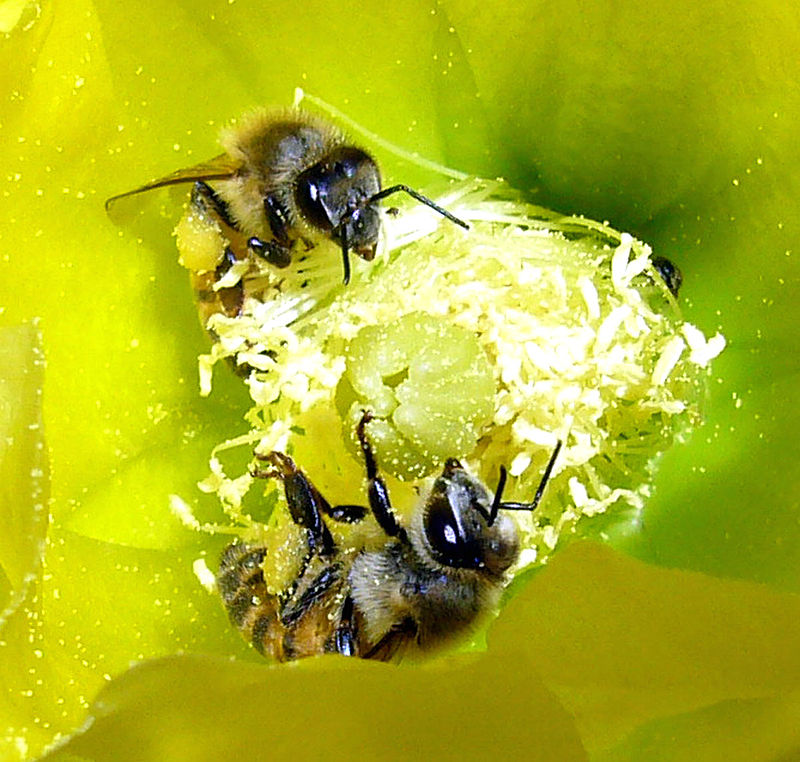
\includegraphics[scale=0.33]{Figures/INTRO_Pollination.jpg}
\caption{\textit{Apis mellifera} libando en una flor de \textit{Opuntia basilaris}, California (Estados Unidos). Fotografía de Jessie Eastland, \small{\texttt{CC BY-SA 3.0}}.}
\label{fig:INTRO_Pollination}
\end{figure}

Las comunidades de plantas y dispersores de semillas funcionan con el mismo esquema de intercambio de alimentación por servicio. Los frugívoros obtienen comida y en compensación reparten las semillas de la planta. Este tipo de mutualismo se registra sobre todo en los trópicos \cite{bascompte2007plant, estrada2012frugivores}.
	
Aunque menos comunes, también hay intercambios de recurso por recurso, como entre la bacterias del tipo \textit{Rhizobium} y las leguminosas a cuyas raíces se fijan. La bacteria proporciona nitrógeno a la planta y se alimenta de los azúcares que esta produce \cite{lindstrom2010biodiversity}.
	
Finalmente, el intercambio de servicio por servicio es la base de simbiosis como la de las anémonas con los peces y crustáceos que se han adaptado a vivir entre sus tentáculos venenoso. La anémona protege al huésped de los depredadores y a cambio este limpia sus parásitos \cite{mebs2009chemical}.

Otra distinción se basa en la \textbf{importancia vital para los actores}. En el \textit{mutualismo obligatorio} cada especie requiere del concurso de la otra para subsistir. Se suelen citar los ejemplos de yuca y sus polillas \textit(Prodixidae) o el ya citado de la anémona, aunque hay dudas de que sean absolutamente obligatorios \cite{briand1982phylogenetic, addicott1995cheating}. Está muy asociado a una gran especialización y coevolución de los mutualistas. En el \textit{mutualismo facultativo}, la relación no tiene ese carácter esencial. Es el más común en las comunidades de plantas y polinizadores \cite{geib2012tracing}.

Una última distinción se basa en la \textbf{recepción directa o indirecta del beneficio}. El \textit{mutualismo directo} es el más común, pero a veces interviene una tercera especie que
intermedia entre las dos. Boucher, James y Keeler exponen diversos ejemplos en su artículo ya citado. Desde un punto de vista de teoría de redes este \textit{mutualismo directo} es una composición de dos pares de relaciones.


\begin{figure}[h!]
\centering
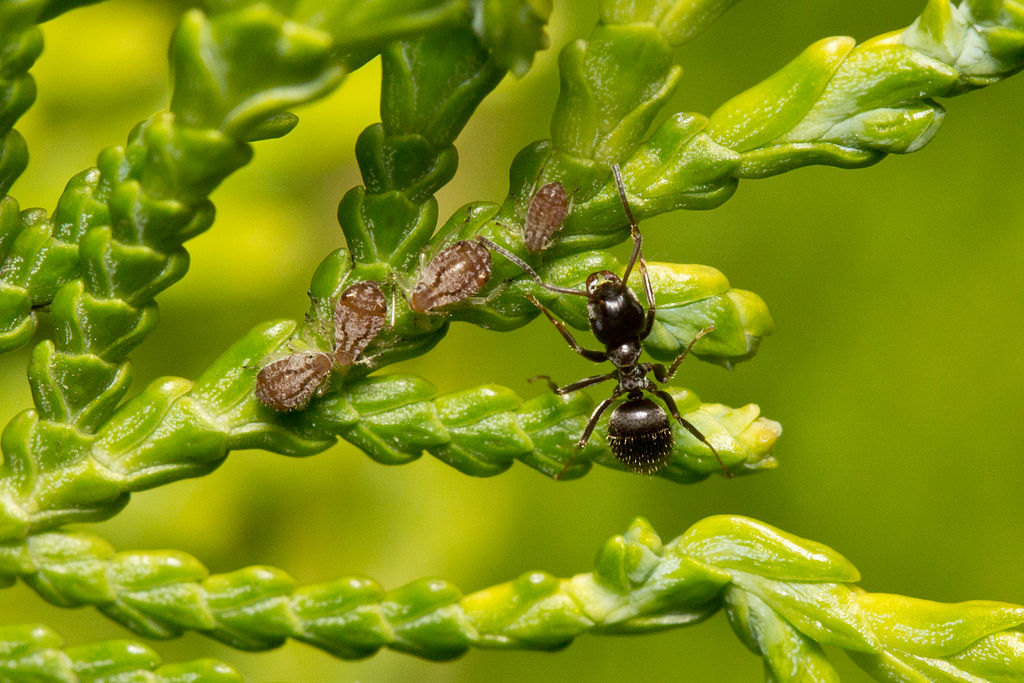
\includegraphics[scale=1]{Figures/INTRO_Lasius_niger_y_Cinara_tujafilina_en_Thuja_occidentalis.jpg}
\caption{\textit{Lasius niger} cuidando de varios ejemplares de \textit{Cinara tujafilina} sobre hojas de la conífera Tuya del Canadá \textit{Thuja occidentalis}. Fotografía de Carlos Delgado, \small{\texttt{CC BY-SA 3.0}}.}
\label{fig:INTRO_Lasius_niger_y_Cinara_tujafilina_en_Thuja_occidentalis}
\end{figure}

Los insectos sociales han desarrollado formas de mutualismo muy elaboradas. En la relación entre hormigas y áfidos se intercambia un servicio (protección) por alimento (ligamaza) \cite{volkl1999ant}. Bajo determinadas circunstancias la relación se transforma en depredación de ejemplares de los primeros por las segundas, con una forma de explotación muy similar a la que se estableció en el Neolítico entre el ser humano y animales domesticados como la oveja. Otras especies cultivan hongos en sus hormigueros \cite{mueller2001origin}, en un comportamiento que también se asemeja a la relación de mutualismo que supone la agricultura.

A veces, las relaciones son complejas. Las hormigas actúan como protectoras de las acacias de las que reciben alimento y también protección contra depredadores con las púas de estos árboles \cite{raine2002spatial}. Las asociaciones entre \textit{mirmecofitas} y hormigas son muy especializadas y de naturaleza simbiótica \cite{djieto2004symbiotic}.También se documenta un tipo de mutualismo indirecto entre robles y hormigas, mediado por áfidos. La abundancia de estos no daña al árbol y beneficia a las hormigas, que a su vez, actúan como defensa frente a insectos que deterioran las bellotas \cite{ito1991indirect}.


%----------------------------------------------------------------------------------------
%	SECTION 2
%----------------------------------------------------------------------------------------

\section{Redes en ecología}

Una red es un conjunto de entidades entre las que se establecen relaciones. Representando las primeras como nodos y las segundas como enlaces, 
se construye un grafo, un modelo abstracto muy versátil. La estructura y dinámica dependen solo de su conformación, no de la realidad que representa. La ciencia de redes es una disciplina de desarrollo reciente que estudia cualquier fenómeno al que pueda aplicarse este método de modelado. Utiliza técnicas propias de la teoría de grafos clásica, de la física estadística o de la sociometría y tiene un amplío espectro de aplicación: economía, biología, tecnología, historia, literatura... \cite{barabasi2002linked, newman2003structure, brandes2013network}

Las redes son ubicuas en biología \cite{mason2007graph, raymond2009network}. Aparecen en las rutas metabólicas, la expresión génica o en epidemiología, por citar tres ejemplos destacados. Las comunidades ecológicas son redes de interacciones y su estudio en calidad de tales es anterior al auge actual de la ciencia de redes. Los investigadores de las cadenas tróficas ("\textit{food webs}") fueron los que abrieron este camino \cite{pimm1982food,martinez1992constant}.

\begin{figure}[h!]
\centering
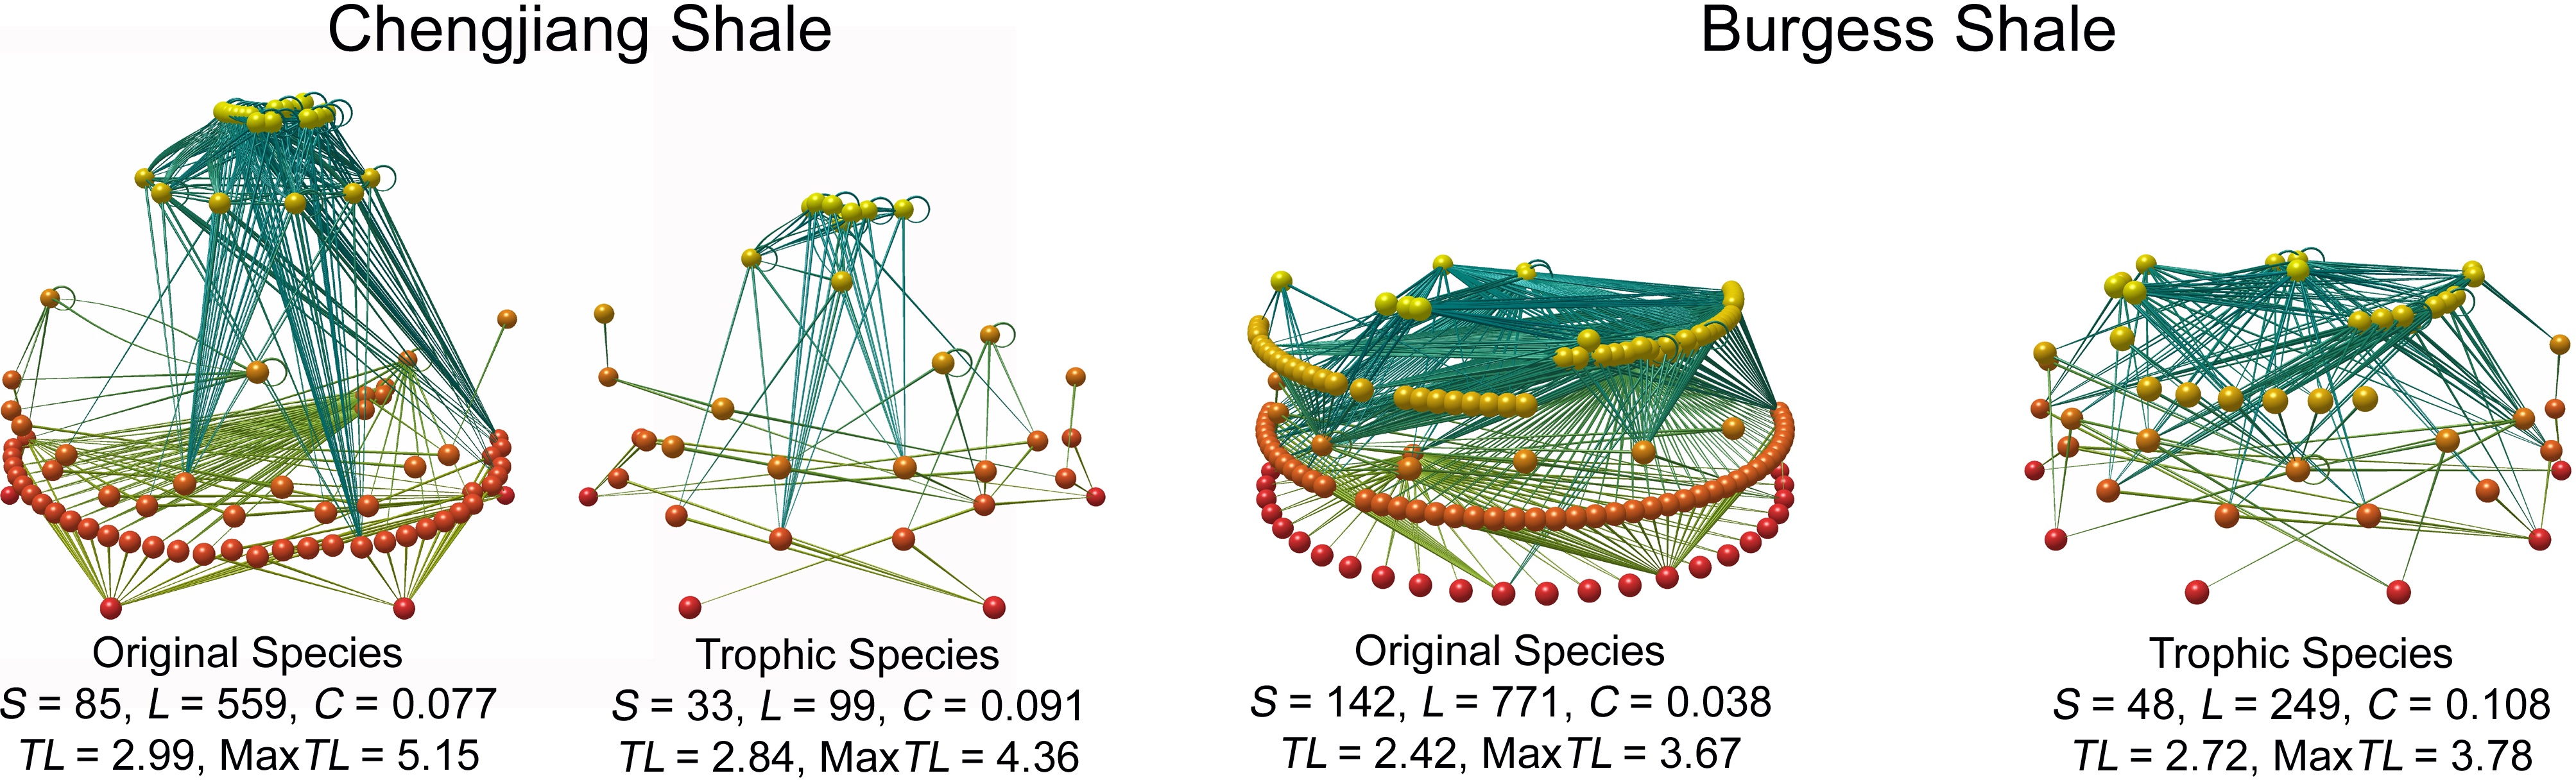
\includegraphics[scale=0.75]{Figures/INTRO_Chengjiang_and_Burgess_Shale_1.png}
\caption{Ejemplo de representación de cadenas tróficas como redes \cite{dunne2008compilation}. \small{\texttt{CC BY-SA 2.5}}.}
\label{fig:INTRO_Chengjiang_and_Burgess_Shale_1}
\end{figure}


\subsection{Redes mutualistas}

Las comunidades mutualistas se pueden modelar, en su forma más general, como redes bipartitas, dirigidas y pesadas. Son bipartitas porque existen dos clases de nodos y las relaciones solo pueden establecerse entre especies de clases distintas. Los enlaces representan el beneficio que la especie $X$ de la clase $A$ aporta a la especie $Z$ de la clase $B$, por tanto son pesados \cite{barrat2004architecture}. La intensidad de este beneficio no es la misma que la que que recibe $X$ de $Z$, de manera que la red es dirigida. La figura \ref{fig:INTRO_bip_ficticia} muestra un diagrama bipartito de una comunidad mutualista. Para hacer más legibles los diagramas reales, la interacción entre dos especies se simplifica como un solo enlace no dirigido.

Una de las objeciones que pueden hacerse al modelado de las comunidades mutualistas como redes es su enfoque reduccionista. Tan solo se incluyen las interacciones positivas entre especies, pero como se ha explicado en el apartado \ref{TIPOS_DE_MUTUALISMO} la realidad puede ser mucho más rica. La simplificación es cierta. La red es una abstracción a la que podrían añadirse otros tipos de relación, posiblemente complicando el modelo hasta hacerlo inmanejable y mezclando los efectos del mutualismo con los de otros tipos de relación ecológica. En este punto conviene recordar la reflexión de George Box que abre la tesis. No hay modelos perfectos, pero algunos resultan útiles. A la vista de los resultados que ha producido esta forma de estudiar el mutualismo, es un modelo útil.

\begin{figure}[h!]
\centering
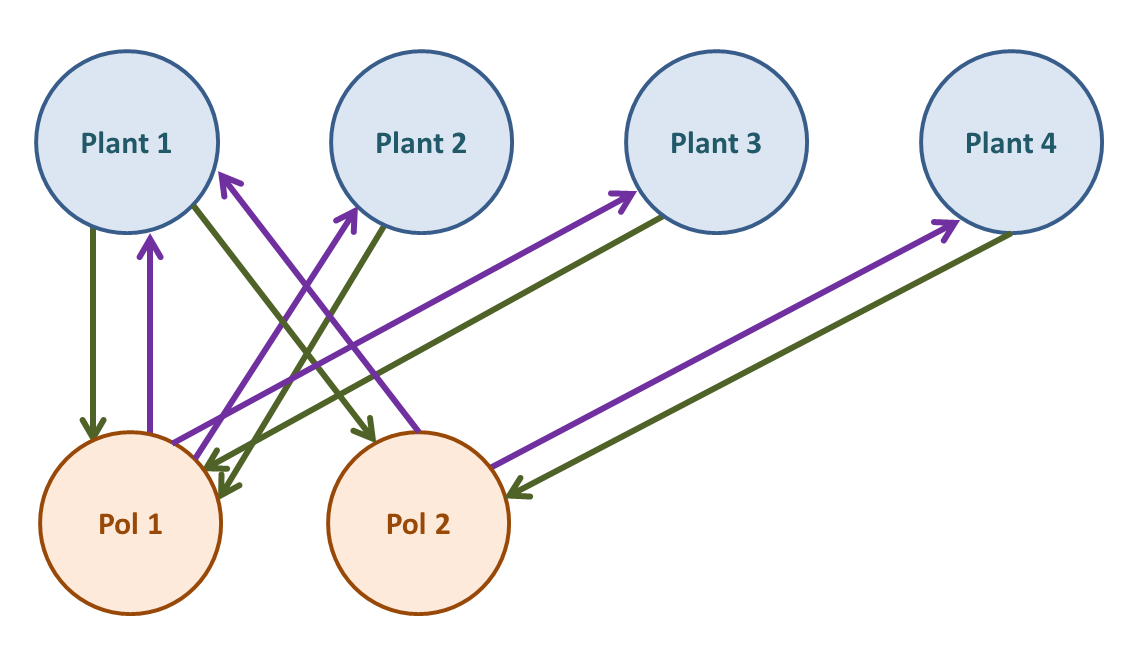
\includegraphics[scale=0.30]{Figures/INTRO_bip_ficticia.png}
\caption{Red mutualista ficticia con cuatro plantas y dos polinizadores}
\label{fig:INTRO_bip_ficticia}
\end{figure}

En su artículo seminal de 1987, Pedro Jordano aplicó de manera sistemática al mutualismo un enfoque de redes, utilizando las medidas que se habían empleado para las cadenas tróficas.

\enquote{\itshape Entender como se distribuyen el número y la fuerza de los enlaces entre los distintos pares de especies es básico para entender la evolución del mutualismo en un determinado contexto} \cite{jordano1987patterns}.

El análisis partía de la \textit{matriz de adyacencia}. Las especies de una clase se disponen como filas y las de la otra como columnas, si existe interacción la casilla de la matriz está rellena (figura \ref{fig:INTRO_M_PL_011a_matrix}). Jordano observó que el número de interacciones crece con el tamaño de la red, como cabía esperar. La \textit{conectancia}, entendida como la fracción del número de enlaces existentes entre todos los posibles presentaba una gran heterogeneidad. A partir de la publicación de este artículo, la literatura sobre redes mutualistas ha conocido un crecimiento sostenido y vive en la actualidad un periodo de florecimiento \cite{gu2015emerging}.

Además de la \textit{conectancia}, se han utilizado medidas habituales en el análisis genérico de redes. La \textit{distribución de grado} representa el número de enlaces por especie, y en las redes \textit{libres de escala} obedece a una ley de potencia. La mayoría de las comunidades mutualistas muestran una ley de potencia truncada \cite{jordano2003invariant}, lo que indica que no se forman de manera puramente aleatoria pero que tampoco se forman por \textit{conexión preferencial} \cite{barabasi1999emergence}. La explicación del mecanismo subyacente es aun objeto de debate pues no está claro si surge por restricciones de base biológica \cite{bascompte2007plant}, por pura estadística \cite{vazquez2005degree} o porque los datos disponibles no son suficientes y pueden tener sesgos de muestreo \cite{okuyama2008mutualistic, williams2011biology}. Por estos inconvenientes la distribución de grado no es la medida más útil en la caracterización del mutualismo.

Otras magnitudes de uso común como el \textit{clustering} o la \textit{distancia media} no son libres de escala, es decir, dependen del tamaño de la red \cite{olesen2006smallest}.

Además de la incertidumbre de los datos disponibles, la formación de las redes ecológicas, y en particular de las mutualistas, parece seguir distintas reglas que la de redes artificiales:

\enquote{\itshape El mecanismo de que los ricos serán más ricos está en contra de los principios ecológicos. Por ejemplo, cuantas más especies de frugívoros se alimenten de una misma especie de fruto, la competencia crecerá y será menos probable que otro frugívoro la incluya en su dieta y, por tanto, se alimentará de otras frutas.} \cite{montoya2006ecological}.

A pesar de todos estos obstáculos, el modelo de redes ha contribuido a avanzar en el estudio del mutualismo con el uso de magnitudes que describen de manera expresiva su estructura como la \textit{modularidad} y el \textit{anidamiento}.
%
%\begin{figure}[h!]
%\centering
%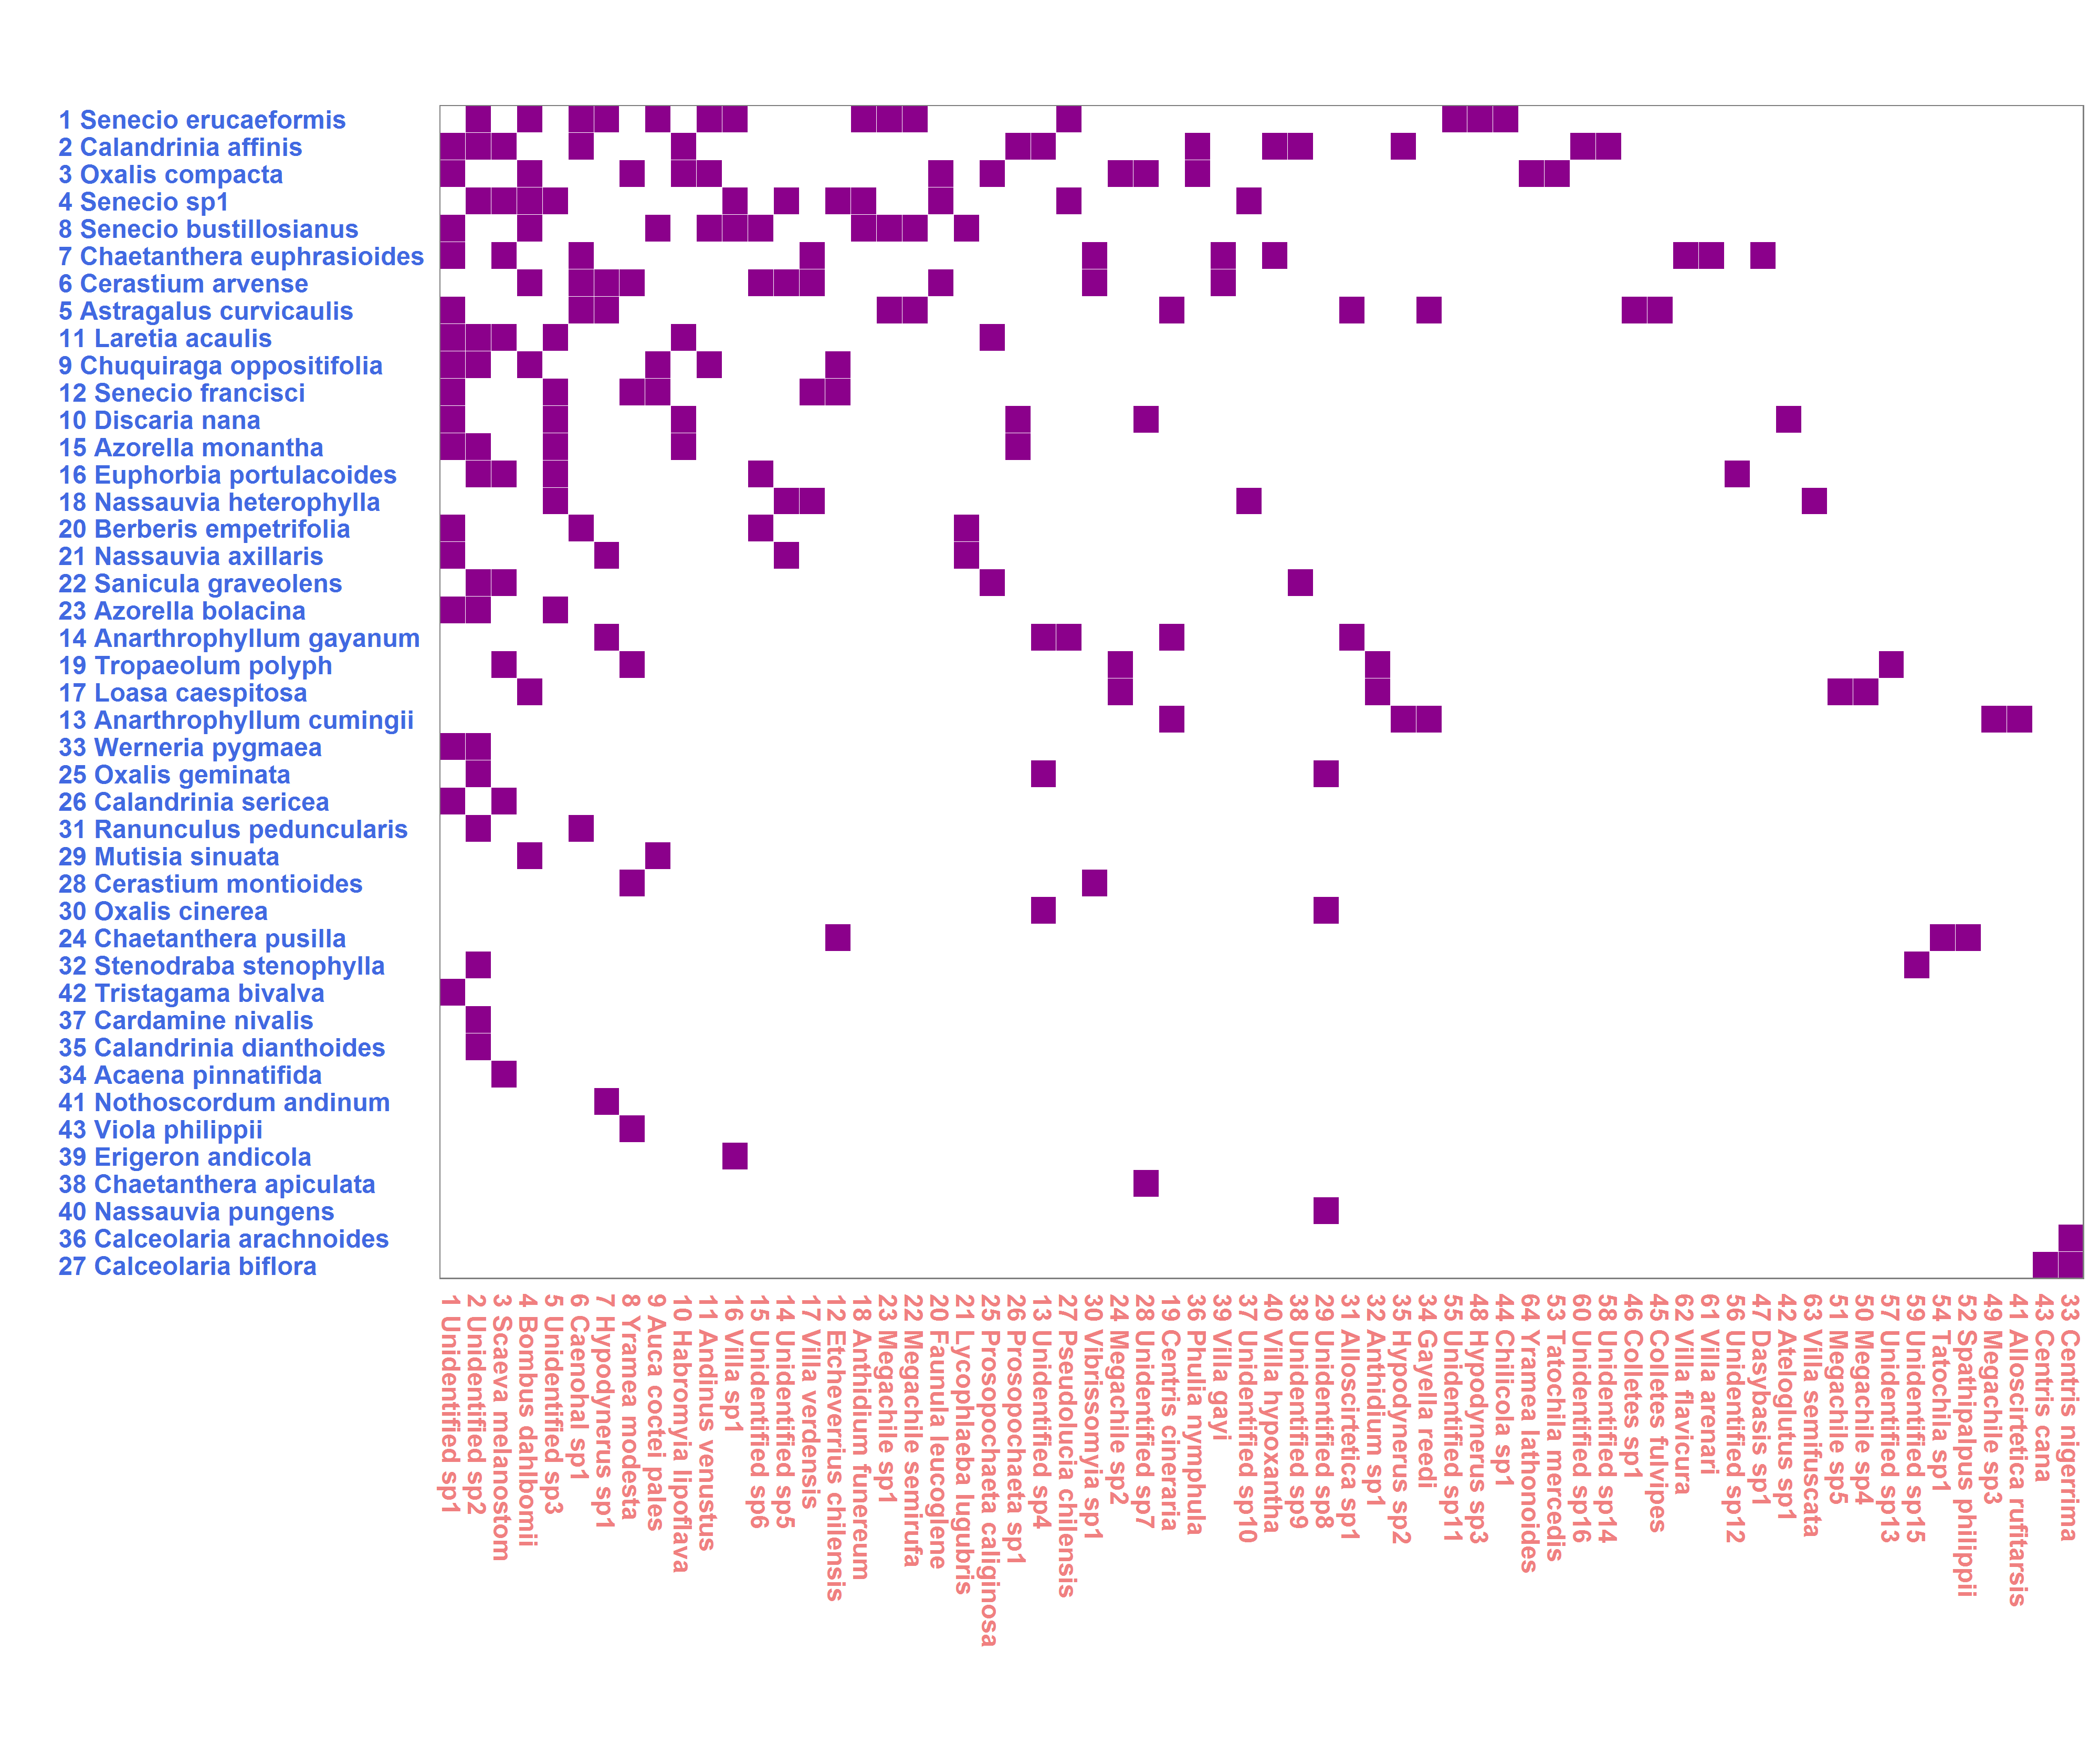
\includegraphics[scale=0.4]{Figures/INTRO_M_PL_002a_matrix.png}
%\caption{Matriz de adyacencia de una red con elevada modularidad. Comunidad de plantas (en azul) y polinizadores (en salmón), Los Andes (Chile) \cite{arroyo1982community}.}
%\label{fig:INTRO_M_PL_002a_matrix}
%\end{figure}

\begin{figure}[h!]
\centering
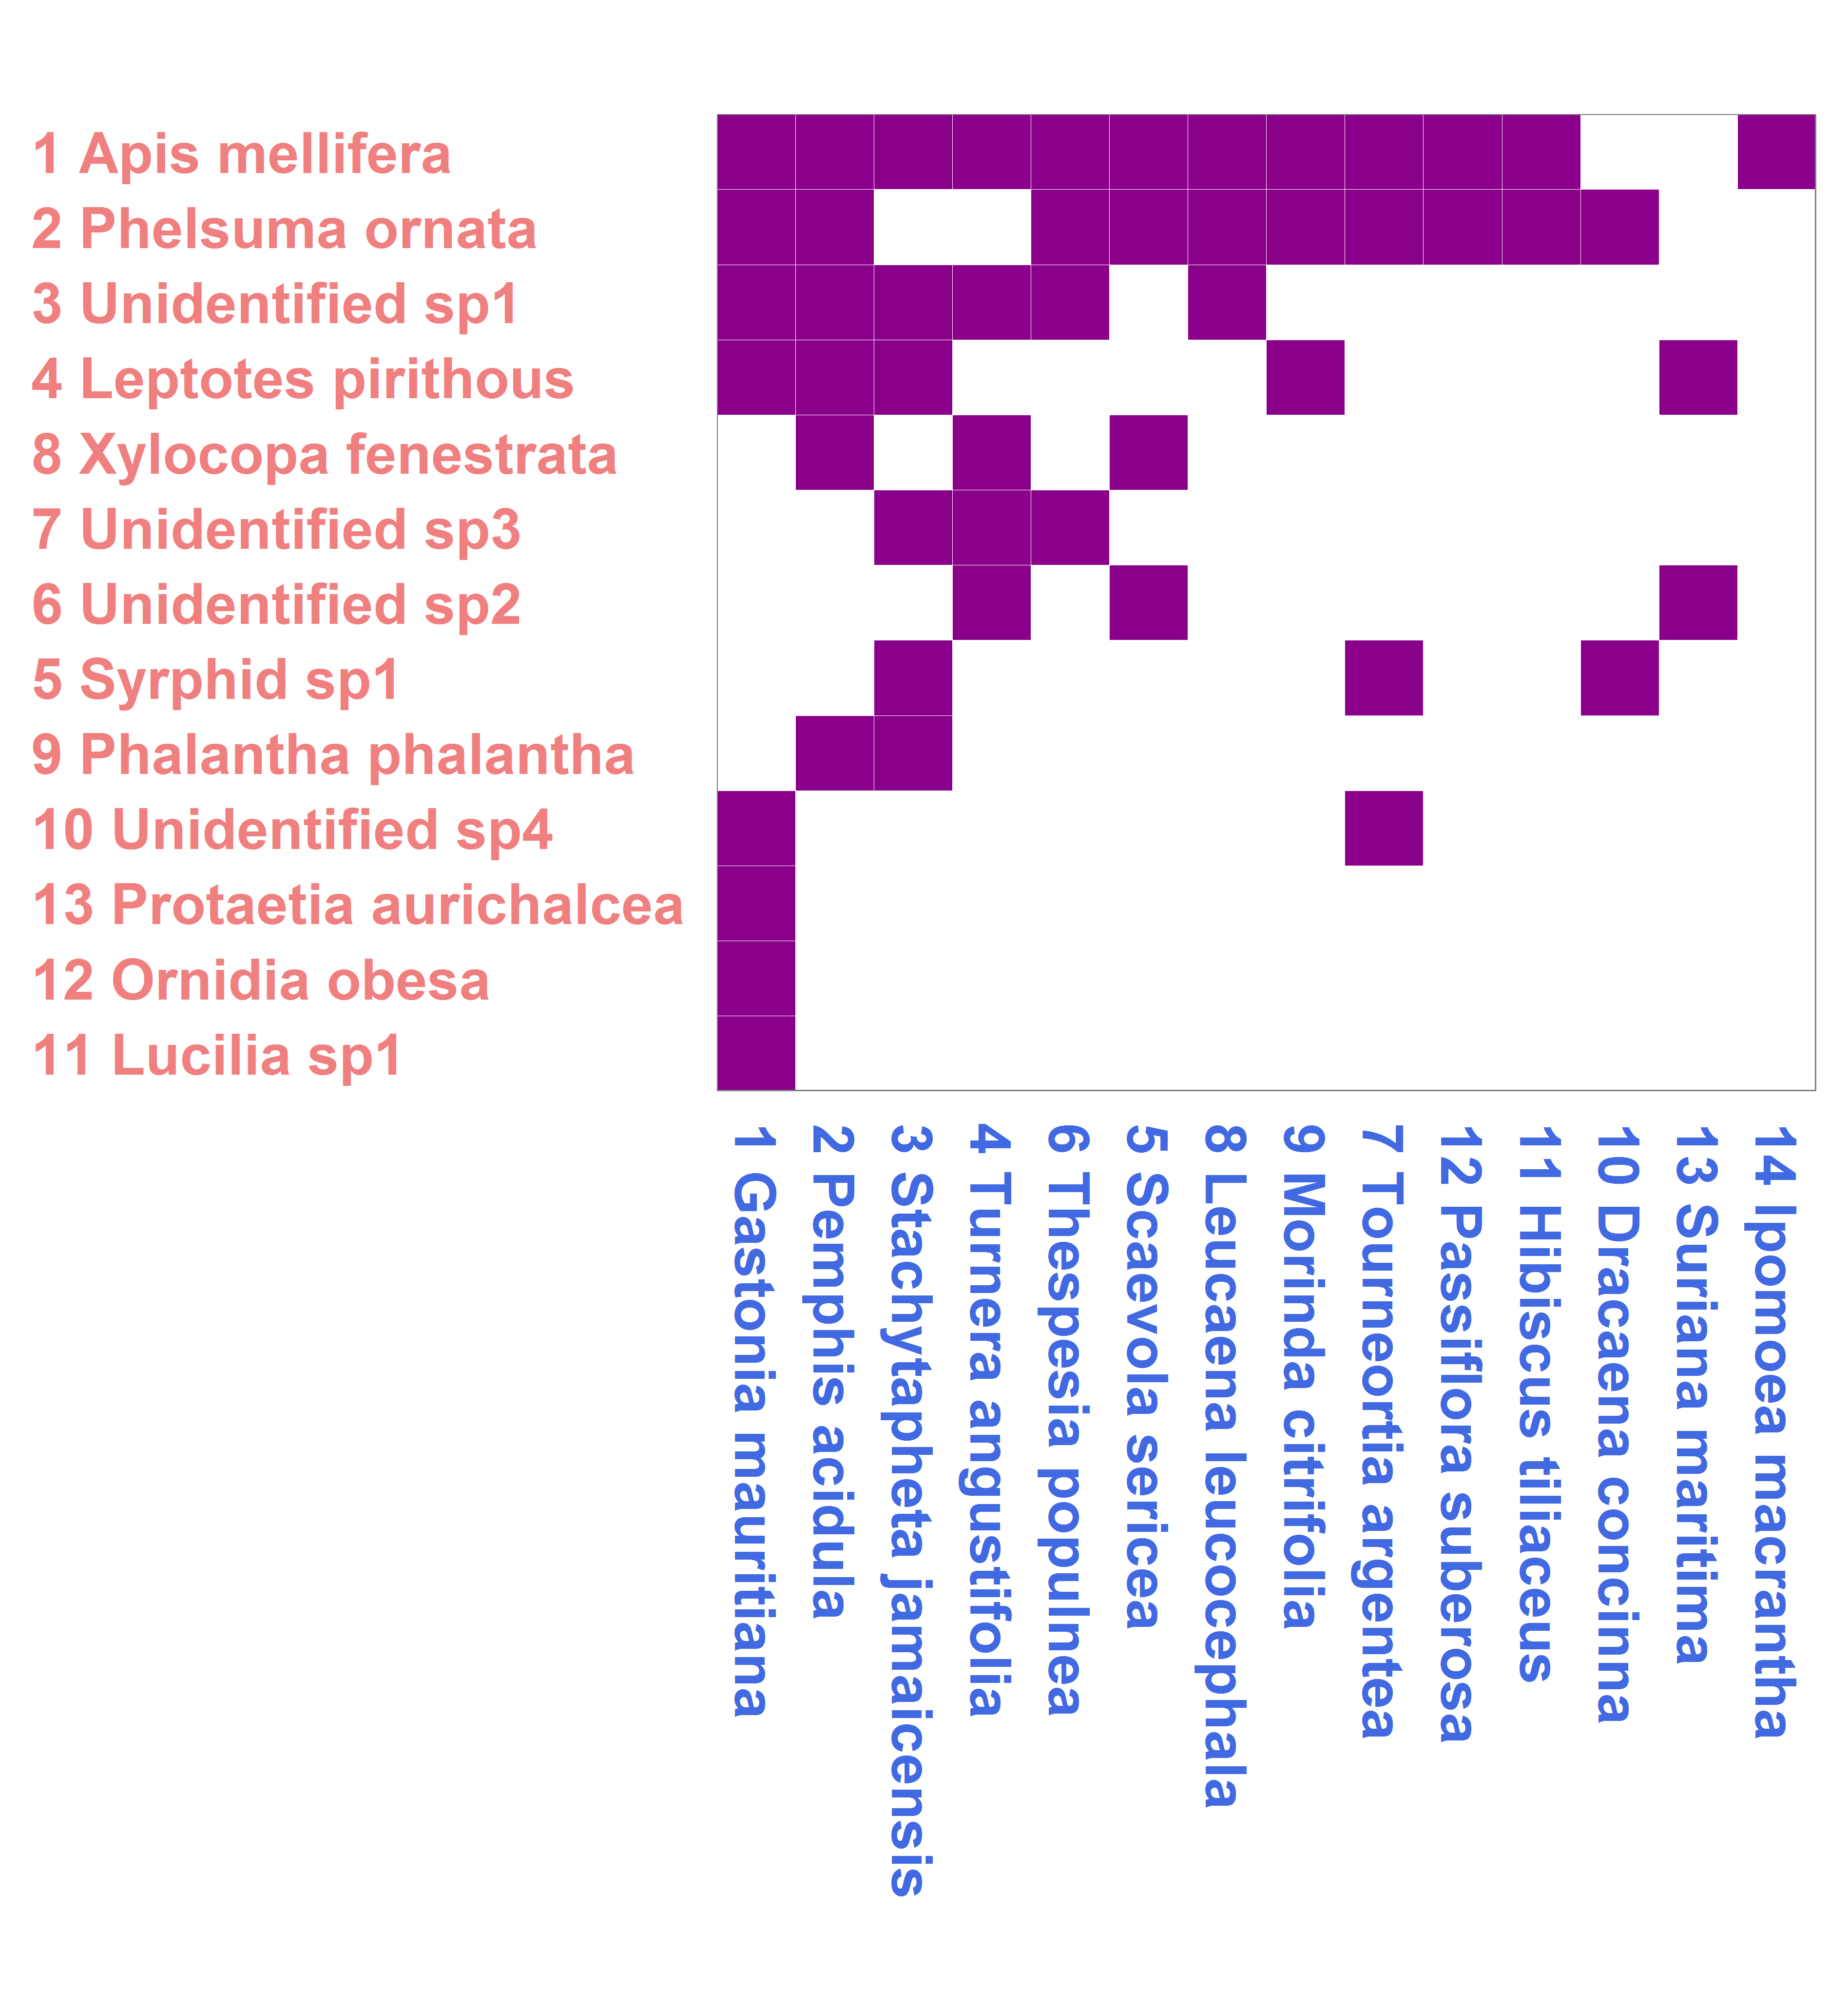
\includegraphics[scale=0.3]{Figures/INTRO_M_PL_011a_matrix.png}
\caption{Matriz de adyacencia de una red mutualista. Comunidad de plantas (en azul) y polinizadores (en salmón), Île aux Aigrettes (Mauricio) \cite{olesen2002invasion}.}
\label{fig:INTRO_M_PL_011a_matrix}
\end{figure}


De una forma intuitiva, la \textit{modularidad} expresa la existencia de conjuntos de nodos muy conectados dentro de una red con una densidad menor \cite{newman2006modularity}. Los módulos aparecen en las redes ecológicas por la existencia de complementariedad funcional entre las especies que los forman y aportan estabilidad frente a las extinciones en cascada \cite{olesen2007modularity, thebault2010stability, stouffer2011compartmentalization}.

El \textit{anidamiento} es una medida de organización jerárquica \cite{atmar1986nested} que resulta muy útil en el estudio del mutualismo. Existe la evidencia empírica de que existe un núcleo de especies muy conectadas entre sí, a las que se denomina \textit{generalistas}, mientras que las \textit{especialistas} con uno o muy pocos enlaces interactuan con las especialistas pero muy raramente entre ellas \cite{bascompte2003nested, krishna2008neutral}.

Existe distintas medidas de anidamiento, que pueden usar la simplificación de tratar la matriz de interacción como binaria (\textit{nestedness temperature calculator} \cite{atmar1995nestedness}, $NODF$ \cite{almeida2008consistent})o manejarla con sus pesos ($WINE$ \cite{galeano2009weighted}). Las conclusiones papel del anidamiento en la formación y estabilidad de las redes mutualistas dependen mucho de la medida empleada, lo que hace que el debate académico sea muy intenso en la actualidad \cite{staniczenko2013ghost, strona2015new}. De lo que no cabe duda es de la riqueza que ha aportado este concepto a la investigación sobre las redes mutualistas.

\section{Dinámica de las comunidades mutualistas}

A pesar de su larga historia, hay aun muchos puntos abiertos en la investigación de la dinámica de poblaciones. Algunos de ellos fueron presentadas en el 125 aniversario de la revista {\em Science} hace ya una década  \cite{kennedy2005,pennisi2005,stokstad2005}. Por ejemplo, los mecanismos que dan origen y mantienen la biodiversidad en un ecosistema son objeto de investigación desde campos diversos por la comunidad científica \cite{williams2000,dunne2002biodiversity,olesen2007modularity,allesina2008,bascompte2009,saavedra2009,bastolla2009,fortuna2010nestedness,encinas2012}.  

El antecente más antiguo del estudio cuantitativo de las poblaciones se remonta a $1202$ cuando Leonardo Pisano (\textit{Fibonacci}), describió en su obra enciclopédica {\em Liber Abaci} la serie que sigue el crecimiento de una población de conejos \cite{sigler2002}. La teoría clásica de poblaciones, no obstante, se remonta a a $1798$ cuando Robert Malthus publicó {\em An Essay on the Principle of Population} \citep{malthus1798}. En dicha obra Malthus razonaba que el crecimiento de la población humana es proporcional al tamaño dado en un momento. Trasladándolo a una ecuación diferencial:
\begin{equation}
\frac{dN}{dt}=r_0\, N 
\label{eq:malthus}
\end{equation}
\noindent donde $N$ es el número de individuos y $r_0$ la {\em tasa intrínseca o vegetativa} de crecimiento de la polación, igual a la diferencia de las tasas de reproducción y defunciones cuando no hay migraciones.

El modelo malthusiano predice un crecimiento exponencial, así que si $r_0 > 0$ no tendría límite. En este modelo $r_0$ permanece constante a lo largo del proceso, sin tener en cuenta factores limitantes como la falta de alimentos o de espacio. En $1838$ Verhulst añadió un término adicional y llamó a su modelo modificado ecuación \emph{logística} \cite{verhulst1845}. La hipótesis de Verhulst es que la tasa de crecimiento debe reducirse conforme $N$ aumenta, hasta alcanzar un máximo. La forma matemática más simple de conseguirlo es haciendo que $r_0$ sea una función lineal de $N$: $ r_0 = r - \alpha N$, donde $r$ es la tasa intrínseca de crecimiento y $\alpha$ un coeficiente positivo de fricción que se interpreta como la competeción entre los individuos de la misma especie por los recursos que permiten su crecimiento y supervivencia. El modelo $r-\alpha$ de Verhulst es:
\begin{equation}
\frac{dN}{dt}=r \, N \,  - \alpha  \, N^2 
\label{eq:primitiveverhulst}
\end{equation}
El término $\alpha$ actúa como un freno biológico, que sitúa al sistema en un punto de equilibrio cuando la población alcanza un valor $ K = r / \alpha$, comúnmente denominado \emph{capcidad de carga}.

Sin embargo, la ecuación logística se conoce mucho más en la forma que Raymond Pearl introdujo en un libro de biometría en $1930$ (véase una excelente reseña histórica en \cite{mallet2012struggle}). En esta formulación, que se impuso en los libros de texto y en la literatura científica, la capacidad de carga aparece como un parámetro explícito de la ecuación y por ello se conoce como la forma $r-K$:

\begin{equation}
\frac{dN}{dt}=r \, N \, \left(1-\frac{N}{K}\right)
\label{pearl}
\end{equation}

La solución de esta ecuación es una curva sigmoide que crece asintóticamente hacia $K$. La fórmula de Pearl tiene algunos inconvenientes matemáticos importantes \citep{kuno1991some,gabriel2005paradoxes}. El más notable es que predice un absurdo crecimiento si la tasa $r$ es negativa pero la población inicial está por encima de la capacidad de carga. Este problema fue señalado por Richard Levins y en consecuencia de denomina \textit{paradoja de Levins}. Es importante señalarlo, porque todos los modelos de mutualismo se han derivado de la logística en la formulación de Pearl y por tanto arrastran este inconveniente.

Para solucionar el problema Levins propuso que $r$ debía ser siempre no negativa. Gabriel \emph{et al.} encontraron una solución más elegante usando la formulación original de Verhulst \cite{gabriel2005paradoxes}. La condición para que el sistema alcance la establidad es que el coeficiente $\alpha$ sea siempre positivo y la capacidad de carga se redefine como:

\begin{equation}
K_{\infty}=\lim_{t\rightarrow\infty}N(t),\; N(0)>0
\end{equation}

\noindent y entonces
\begin{equation*}
K_{\infty}=\left\{
\begin{array}{ll}
  \alpha / r = K, & \mathrm{si} \;\; \alpha > 0, \\ 0  & \mathrm{si} \;\; \alpha \le0 \\
  \end{array} \right.
\end{equation*}

Estos modelos primitivos de dinámica no incluían interacciones entre especies. Cuando varias de ellas comparten un mismo ecosistema aparece una compleja cadena de relaciones que puede modelarse como una red, como se mencionó en la introducción. En $1926$ Vito Volterra propuso un modelo de dos especies para explicar el comportamiento de algunos bancos de pesca en el Adriático \cite{volterra1926}. Las ecuaciones de Volterra describen las poblaciones de presa $N(t)$ y depredador $P(t)$ de la siguiente manera: 
\begin{align}
%\begin{split}
\displaystyle &\frac{dN}{dt}=N\, \left(a-b \,P\right) \nonumber\\
\displaystyle &\frac{dP}{dt}=P\, \left(c\, N-d\right) 
\label{myeq1}
%\end{split}
\end{align}
\noindent donde $a$, $b$, $c$ y $d$ son constantes positivas. En el modelo de Lotka-Volterra, como se conoce hoy, el crecimiento de la población de la presa está limitado por la población del derpedador y viceversa. Este par de ecuaciones tiene una solución oscilatoria.

El mutualismo, probablemente porque es una interacción menos abundante en la naturaleza, ha recibido menos atención históricamente, también desde el punto de vista matemático. El primer modelo fue propuesto por Richard May. Las ecuaciones de May representan una ecuación logística a la que se ha añadido un tercer término que representa el beneficio mutualista. Es la misma idea que la del modelo Lotka-Volterra, pero con un inconveninete analítico, las interacciones son siempre positivas, de manera que no hay oscilaciones y sí la posibilidad de un crecimimento ilimitado. El modelo de May se formaliza como:
\begin{align}
\frac{dN_1}{dt}=r_1 \,N_1\,\left(1-\frac{N_1}{K_1}\right)+r_1\, N_1\,\beta_{12}\, \frac{N_2}{K_1} \nonumber \\ 
\frac{dN_2}{dt}=r_2\, N_2\, \left(1-\frac{N_2}{K_2}\right)+r_2\, N_2\, \beta_{21} \, \frac{N_1}{K_2} 
\label{myeq2}
\end{align}
\noindent donde $N_1(N_2)$ es la población de la especie $1(2)$; $r_{1,2}$ es la tasa vegetativa de la población $1\, (2)$ y $K_1\, (K_2)$ la capacidad de carga. Este es el máximo que el entorno puede mantener en función de la disponibilidad de sustento y espacio. Por último, $\beta_{12}\,(\beta_{21})$ es el coeficiente que representa el beneficio mutualista para la especie $1\,(2)$ de su interacción con la $2\,(1)$. El principal inconveniente del modelo de May es que conduce a crecimiento ilimitado. No obstante, ha servido de inspiración para todos sus sucesores que incorporan términos adicionales para solucionar este problema.

Ha habido diferentes estrategias de ataque. Wright propuso un modelo de dos especies con saturación como resultado de las restricciones del \textit{handling time}, $T_H$, que corresponde al tiempo necesario para procesar los recursos (comida) producidos por la relación mutualista \cite{wright1989}. Esto dio lugar a la familia de modelos conocida como \textit{tipo II}:
\begin{align}
\frac{dN_1}{dt}=r_1\, N_1\, - \alpha_1 \, N_1^2+ \frac{a\, b\, N_1\,N_2}{1+ a\, N_2\,T_H} \nonumber\\
\frac{dN_2}{dt}=r_2\, N_2\, - \alpha_2 N_2^2 + \frac{a\,b\,N_1\,N_2}{1+a\, N_1\, T_H}
\label{eq_typeII}
\end{align}
\noindent donde $a$ es la tasa efectiva de búsqueda y $b$ un coeficiente que tiene en cuenta los encuentros entre individuos de las especies $1$ y $2$. La dinámica del modelo depende en gran medida del afinado de los parámetros, pero para un rango limitado de ellos muestra tres puntos fijos. Uno estable, que corresponde con la destrucción completa, otro también estable en máximos de población y un \textit{saddle} que separa las cuencas de atracción de los dos primeros. Usando un modelo tipo II, Bastolla demostró la importancia de la estructura de la red para minimizar la competencia entre especies y optimizar la biodiversidad \cite{bastolla2005,bastolla2009}. Los modelos de tipo II son, no obstante, difíciles de manejar analíticamente, debido a la forma en fracción del término mutualista. Hay otras alternativas recientes \cite{johnson2013} que proponen añadir términos adicionales al modelo tipo II, dificultando aun más el análisis.


\section{Cuestiones abiertas en el modelado del mutualismo}

Phasellus fermentum magna in augue gravida cursus. Cras sed pretium lorem. Pellentesque eget ornare odio. Proin accumsan, massa viverra cursus pharetra, ipsum nisi lobortis velit, a malesuada dolor lorem eu neque.

\section{Objetivos}

En esta tesis desarrollaremos aportaciones teóricas y computacionales al modelado del mutualismo en ecología con las siguientes metas:

\begin{enumerate}
\item Construir modelos dinámicos alternativos que eviten las limitaciones conocidas de los actuales.
   \begin{enumerate}
		\item Deben limitar las poblaciones bajo cualquier circunstancia.
		\item Evitarán los problemas derivados de la formulación de Pearl.
		\item Permitirán una explicación biológica de sus propiedades analíticas.
   \end{enumerate}
   
\item Describir las propiedades estructurales de las redes mutualistas basada únicamente en su topología.
		\begin{enumerate}
		\item Las magnitudes deberán explicar las propiedades del mutualismo tanto a escala local como a escala global.
		\item Se establecerá la relación de las citas propiedades topológicas con los índices más habituales en la descripción de las redes mutualistas.
		\end{enumerate}
		
\item Construir nuevos tipos de visualización que superen las limitaciones del diagrama bipartito y de la matriz de interacción para el tamaño habitual de las redes reales.

\item Estudiar la resistencia de las redes mutualistas y las posibles políticas de conservación a la luz de su caracterización topológica.
\begin{enumerate}
		\item Comparar los criterios de ordenación existentes con los que surjan del desarrollo de la tesis.
		\item Validar los resultados con un conjunto amplio de redes reales.
		\end{enumerate}
		
\item Publicar en modalidad \textit{Open Source} todo el software desarrollado con dos propósitos.
 \begin{enumerate}
		\item Reproducibilidad de los resultados obtenidos para su validación, crítica o refutación por otros investigadores.
		\item Poner en manos de la comunidad científica las herramientas que permitan aprovechar los resultados teóricos de este trabajo.
		\end{enumerate}
\end{enumerate}


\section{Estructura de la tesis}

La tesis se divide en cinco capítulos además de este de introducción. En el capítulo \ref{chapterDINAMICA} se exponen dos modelos dinámicos alternativos al más utilizado en la literatura reciente, el denominado \textit{tipo II}. El primero funciona con capacidad de carga (\textit{carrying capacity}) constante. El segundo, con saturación del beneficio mutualista.

El capítulo \ref{chapterESTATICA} es un análisis de la estructura de las redes mutualistas basado en una técnica clásica de teoría de grafos, la \textit{descomposición k-core}. Esta herramienta permite definir medidas locales y globales de centralidad de las especies, basándose exclusivamente en propiedades topológicas.

Las visualizaciones de redes mutualistas habituales no funcionan bien a partir de unas pocas decenas de especies. Las \textit{k magnitudes} definidas  en el capítulo \ref{chapterESTATICA} son la base para la construcción de dos nuevos tipos de gráfico, tal y como se explica en el capítulo \ref{chapterVISUALIZACIONES}.

En el capítulo \ref{ChapterDESTRUCCION} se realiza un estudio estático de la resistencia de las redes mutualistas. En él se comparan los índices de ordenación más populares con los que surgen de la \textit{k estructura} de las redes.

En el capítulo \ref{chapterCONCLUSIONES} se elaboran las conclusiones de la tesis.

Cierran la memoria los manuales de usuario de las dos aplicaciones desarrolladas.


\section{Anexo: Información sobre este documento}
\label{INTROGEN_ANEXO_KConst}

Esta memoria se ha escrito en \texttt{LaTeX} utilizando como base el fichero de clase desarrollado por Steve Gunn y Sunil Patel, que puede descargarse desde \url{http://www.latextemplates.com/}.

Toda el historial de edición se ha registrado con \texttt{git}. Los ficheros fuente pueden descargarse libremente desde \texttt{github} usando el comando:

\fontsize{3.5mm}{3.5mm}\selectfont
\begin{verbatim}
     git clone https://github.com/ghostdatalearner/texto_tutto.git
\end{verbatim}
\normalsize

% Chapter Template

\chapter{Modelado dinámico} % Main chapter title

\label{chapterDINAMICA} % Change X to a consecutive number; for referencing this chapter elsewhere, use \ref{ChapterX}

%----------------------------------------------------------------------------------------
%	SECTION 1
%----------------------------------------------------------------------------------------

\section{Dinámica de las comunidades mutualistas}

En el capítulo anterior se han expuesto algunos de los problemas que tienen los modelos actuales de dinámica del mutualismo. Además de las limitaciones que se derivan de cada simplificación matemática hay una más grave para verificar la realidad de las predicciones. El peso de los coeficientes $b_{ij}$ de las matrices de interacción es muy difícil de determinar a partir de las observaciones de campo. Las comunidades complejas no pueden reproducirse en laboratorio para obtener medidas precisas por lo que se trabaja con el número de interacciones observadas como indicador. Esta solución no es del todo satisfactoria pero es la mejor de la que se dispone \cite{olesen2002geographic}. 

La imposibilidad de validar los modelos con series de datos de campo de periodos prolongados hace que este campo de estudio siga siendo dominio de la teoría. En este capítulo se proponen dos modelos alternativos de dinámica. El primero se basa en la formulación de Pearl y se garantiza la estabilidad forzando a que la capacidad de carga sea constante. El segundo se aparta de lo publicado hasta la fecha y vuelve la vista a la formulación $r-\alpha$ de la ecuación de Verhulst.

\section{Modelo con capacidad de carga constante}

La primera solución para evitar un crecimiento ilimitado, como el que aparece en las ecuaciones de May, es la base de nuestro modelo con capacidad de carga constante. Desde el punto de vista ecológico, esta solución puede resultar ingenua puesto que el mutualismo supone un incremento de recursos. No obstante, resuelve los problemas descritos en la introducción y es de gran simplicidad.

La ecuación de Verhulst enunciada en el formalismo de Pearl es:

\begin{equation}
\frac{dN}{dt}=r_{\rm{pc}} \, N \, , \; \;\, r_{\rm{pc}}=r\, \left(1-\frac{N}{K}\right)
\label{eq:Verhulst2}
\end{equation}

\noindent  donde la tasa per cápita $r_{\rm{pc}}$ representa el crecimiento por individuo. Se puede entender como una tasa intrínseca 
modificada por un factor adimensional. En la ecuación \ref{eq:Verhulst2} dicho factor incluye el término negativo que representa una
competencia de los individuos de la misma especie, de valor constante y que actúa como freno biológico al crecimiento ilimitado. Esta
es la teoría clásica aunque la dinámica observada en la naturaleza es más compleja \cite{johnson2013}.

Como ya se ha explicado, la fórmula de Pearl solo funciona correctamente para tasas positivas de crecimiento vegetativo si la población
es inferior a la capacidad de carga. La figura \ref{fig:r_equiv_Verh+modif}a muestra la tasa de crecimiento per cápita para diferentes valores de la tasa de
crecimiento vegetativo $r$. La competencia intra especies debería reducir siempre ese valor.

La ecuación logística con esta fórmula predice un crecimiento biológicamente absurdo si $r<0$ y la población está por encima de $K$. En esas condiciones el término $\left(1-\frac{N}{K}\right)$ se vuelve negativo y no modela de manera adecuada el comportamiento real del sistema. 

Para solucionar esta limitación, proponemos una modificación simple en la fórmula de Pearl, que es utilizar el valor absoluto de la tasa vegetativa.

\begin{equation}
\frac{dN}{dt}= N \, \left(r - |r|\,    \frac{N}{K}\right)= r\,N \,\left(1-sgn(r)\,\frac{N}{K}\right)
\label{eq:Verh_r}
\end{equation}

\noindent done $r$ es la citada tasa vegetativa de crecimiento, definida como la diferencia entre las tasas de reproducción y mortalidad ($r=\left(r_{b}-r_{d}\right)$). Este artificio matemático (uso del valor absoluto) da sentido biológico al término de competencia intra específica, que debe ser negativo siempre.

La dinámica de la población de la especie $i$ se puede escribir como:

\begin{equation}
\displaystyle \frac{dN_i}{dt}=\left(r_{b_i}-r_{d_i}\right) N_i - |r_{b_i}-r_{d_i}| \frac{N^2_i}{K_i}
\label{ec:vhoptionI}
\end{equation}

Si $r_b > r_d$ no hay diferencia con la formulación habitual del modelo de Pearl. El término cuadrático es siempre negativo y eso implica la reducción de la población. La ecuación también predice correctamente el comportamiento cuando $N>K$. Cuanto mayor sea la población, la tasa de crecimiento es menor, incluso si $r_b < r_d$. En la figura \ref{fig:r_equiv_Verh+modif} se puede ver una comparativa de la tasa de crecimiento en la formulación de Pearl y de la del modelo modificado de la ecuación \ref{ec:vhoptionI}. La figura \ref{fig:r_equiv_Verh+modif}a muestra la tasa de crecimiento para distintos valores de la tasa vegetativa entre $r=-0.8$ y $r=0.8$.
 
 
\begin{figure}[ht]
\centering
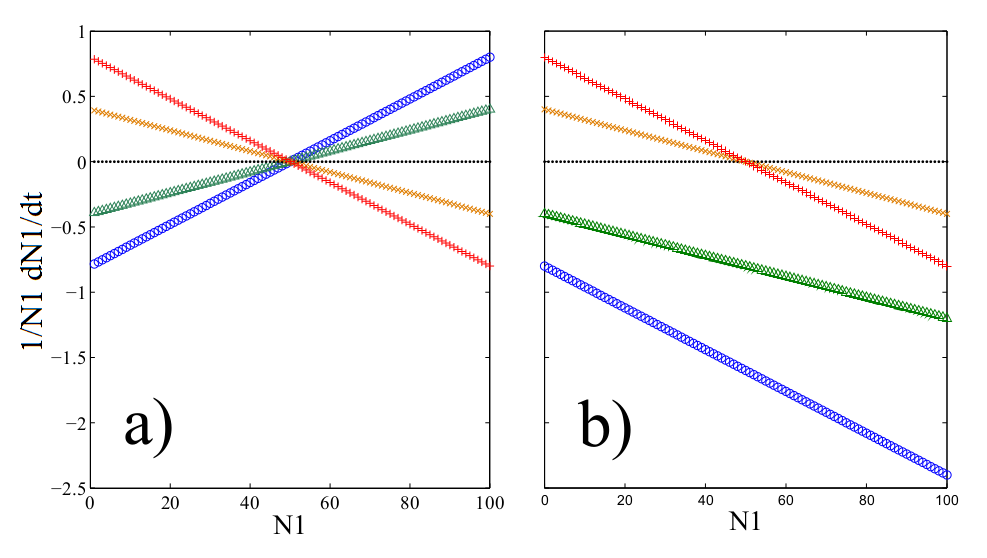
\includegraphics[scale=0.52]{DINAMICA_r1_Verh+modif_r1-p8p8K50.png}
\caption{a) Tasas de crecimiento per cápita para la ecuación logística en la fórmula de Pearl, para las tasas vegetativas $r=-0.8$ (azul)
$r=-0.4$ (verde), $r=0.4$ (naranja) y $r=0.8$ (rojo). b) La misma gráfica para la ecuación modificada de nuestro modelo.}
\label{fig:r_equiv_Verh+modif}
\end{figure}

Por su parte, la figura \ref{fig:r_equiv_Verh+modif}b muestra la tasa de crecimiento para nuestra fórmula modificada. En este caso la tasa per cápita disminuye siempre con el aumento de la población. Basados en esta idea proponemos un modelo de dinámica con capacidad de carga constante.

En el modelo de May se asume que la capacidad de carga y la tasa de crecimiento intrínseca de las especies son constantes e independientes del término mutualista. El efecto del mutualismo es un incremento de la tasa de crecimiento efectiva.

Para el sistema más simple posible, con una especie de cada clase, reescribimos el modelo de May:

\begin{align*}
\displaystyle & \frac{dN_1}{dt}= N_1 \, r_1\, \left(1 + \beta_{12}\frac{N_2}{K_1} \right) \, \left(1-\frac{N_1}{K_1}\right) \\
\displaystyle & \frac{dN_2}{dt}=N_2 \, r_2\, \left(1 + \beta_{21}\frac{N_1}{K_2} \right) \, \left(1-\frac{N_2}{K_2}\right)
\stepcounter{equation}\tag{\theequation}
\label{myeq3}
\end{align*}

El término dentro del primer paréntesis es un factor multiplicativo de la tasa vegetativa, siempre positivo y mayor que $1$.
Ahora podemos reescribir las \textit{tasas de crecimiento eficaces} como:

\begin{align*}
\displaystyle r_{\rm{eq},1}=r_1 + r_1\, \beta_{12} \frac{N_2}{K_1}\, =\, r_1 + b_{12}N_2  \\
\displaystyle r_{\rm{eff},2}=r_2 + r_2\, \beta_{21} \frac{N_1}{K_2}\, =\, r_2 + b_{21}N_1 \stepcounter{equation}
\tag{\theequation}
\end{align*}

Y con esta definición podemos reescribir:

\begin{align*}
\displaystyle & \frac{dN_1}{dt}= (r_1 + b_{12}\, N_2) \, N_1\,\left(1-\frac{N_1}{K_1}\right)=r_{\rm{eff},1}\,N_1\,\left(1-\frac{N_1}{K_1}\right) \\
\displaystyle & \frac{dN_2}{dt}= (r_2 + b_{21}\, N_1) \, N_2\,\left(1-\frac{N_2}{K_2}\right)=r_{\rm{eff},2}\,N_2\,\left(1-\frac{N_2}{K_2}\right)
\stepcounter{equation}\tag{\theequation}
\label{eq:May_reff}
\end{align*}

En ausencia de mutualismo se convierte en la ecuación logística modificada. El factor $\left(1-\frac{N_{1}}{K_{1}}\right)$ limita el crecimiento de la especie $1$ a la capacidad de carga $K_{1}$, y lo mismo sucede con la especie $2$, sin importar cual es la intensidad del mutualismo.

\begin{figure}[t]
\centering
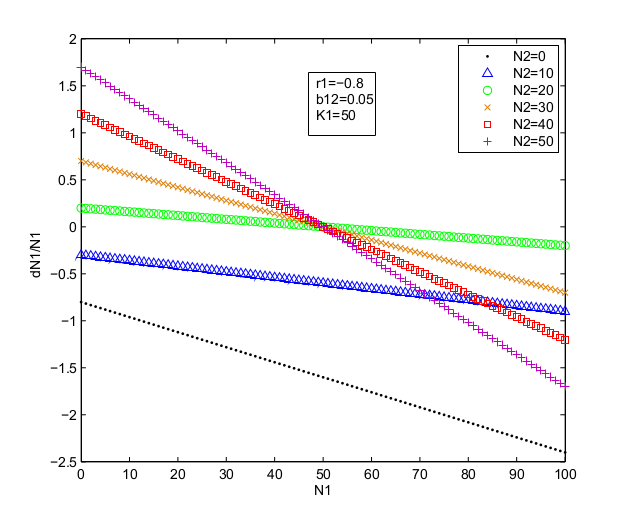
\includegraphics[scale=0.66]{DINAMICA_r1_eq_N1N2_r1p8b12p05K50.png}
\caption{Crecimiento per cápita de la especie $1$ con tasa de crecimiento vegetativa $r_1=-0.8$, capacidad de carga $K_1=50$, y coeficiente de interacción $b_{12}=0.05$, para diferentes valores de población: $N_2=0,10,20,30,40,50$.}
\label{fig:per capita_growth_rate_mutualism}
\end{figure}

Incluyendo la modificación usada en las ecuaciones \ref{eq:May_reff}, nuestro modelo se puede escribir como:
\begin{align*}
\displaystyle & \frac{dN_1}{dt}= N_{1} \left( r_{\rm{eff},1}- |r_{\rm{eff},1}| \frac{N_1}{K_1} \right) = r_{\rm{eff},1}\, N_1 \left(1-sgn(r_{\rm{eff},1})\frac{N_1}{K_1}\right)\\
\displaystyle & \frac{dN_2}{dt}= N_{2} \left( r_{\rm{eff},2}- |r_{\rm{eff},2}| \frac{N_2}{K_2} \right)= r_{\rm{eff},2}\, N_2 \left(1-sgn(r_{\rm{eff},2})\frac{N_2}{K_2}\right)
\stepcounter{equation}\tag{\theequation}\label{eq:new_model}
\end{align*}

Como ya se ha indicado, la función $sgn(r_{\rm{eff}})$ tiene sentido biológico porque la competencia intra especie debe ser siempre negativa, con independencia del signo de la tasa vegetativa.

Para llegar a la fórmula final, generalizamos a una comunidad con $n$ especies de la clase $P$ (plantas), y $m$ especies de la otra $A$ (animales), que se relacionan por medio de una red de interacciones bipartita, pesada y bidireccional. Tomemos una especie $i$ de $P$ de población $N_i$ y otra $j$ de $A$ con $N_j$ individuos. Los pesos de la red representan la tasa de beneficio que recibe la población $i$ por la existencia de $j$. 

Las expresiones de las tasas de crecimiento de las especies $i$, $j$ quedan:
\begin{align*}
\displaystyle & r_{\rm{eff},i}  = \left( r_{b\, i} - r_{d\, i} \right) + \sum\limits_{k=1}^{m} b_{ik}\, N_k  \\
\displaystyle & r_{\rm{eff},j}  = \left( r_{b\, j} - r_{d\, j} \right) + \sum\limits_{l=1}^{n} b_{jl}\, N_l
\stepcounter{equation}\tag{\theequation}\label{modelors}
\end{align*}

Y el modelo con capacidades de carga constantes queda así:

\begin{theo}
\begin{align*}
\displaystyle
&\frac{dN_i}{dt}=r_{\rm{eff},i}\, N_i - |r_{\rm{eff},i}| \, \frac{{N_i}^2}{K_i}  \\
\displaystyle
&\frac{dN_j}{dt}=r_{\rm{eff},j} \, N_j - |r_{\rm{eff},j}| \, \frac{{N_j}^2}{K_j}
\stepcounter{equation}\tag{\theequation}\label{eq:modelo_optionI}
\end{align*}
\end{theo}

\noindent donde en el subíndice $i$ corresponde a las especies de la clase $P$ y $j$ a las de la clase $A$. El término $r_{\rm{eff},i} - |r_{\rm{eff},i}| \frac{N_i}{K_i}$ es la tasa de crecimiento per cápita de la especie $i$, incluyendo los efectos del mutualismo y de la competencia intra especie. La figura \ref{fig:per capita_growth_rate_mutualism} es la tasa per cápita de la especie $1$ (en un sistema mutualista de $1+1$ especies),
con tasa vegetativa negativa $r_1=-0.8$ y coeficientes mutualistas $b_{12}=0.05$ y $K_1=50$, para los siguiente valores de población de la especie$N_2=0,10,20,30,40,50$. Para $N_2=20$, la tasa eficaz es todavía negativa, lo que conduciría a la destrucción del sistema. Para
$N_2=30$ la tasa ya es positiva y el sistema alcanzaría el máximo vital con las poblaciones en $K1$ y $K2$.

\subsection{Análisis de estabilidad para dos especies}

Para ver el comportamiento dinámico de nuestro modelo, vamos hacer un estudio de estabilidad lineal con sólo dos especies (supongamos que la que llamamos $1$ es una planta la que llamamos $2$ un animal, sin pérdida de generalidad). Las ecuaciones del modelo son:
\begin{align*}
\displaystyle \frac{dN_1}{dt}= N_1 \left( r_{\rm{eff},1} - |r_{\rm{eff},1}| \frac{N_1}{K_1} \right) \\
\displaystyle \frac{dN_2}{dt}= N_2 \left( r_{\rm{eff},2} - |r_{\rm{eff},2}| \frac{N_2}{K_2} \right)
\stepcounter{equation}\tag{\theequation}\label{eq:two_species_model}
\end{align*}

\noindent donde $K_1$ and $K_2$ son las capacidades de carga. Las tasas de crecimiento efectivas son:
\begin{align*}
\displaystyle &r_{\rm{eff},1} = r_{1} + b_{12}\, N_2 \\
\displaystyle &r_{\rm{eff},2} = r_{2} + b_{21}\, N_1
\stepcounter{equation}\tag{\theequation}\label{eq:two_species_reff}
\end{align*}

En el sistema \ref{eq:two_species_model} se pueden identificar cinco puntos fijos:
la destrucción total ($N_1=0$,$N_2=0$), con independencia del valor de $r_{1}$ y $r_{2}$;
el máximo vital ($N_1=K_1$,$N_2=K_2$) que aparece si $r_{2}>0$ y $r_{1}>0$ simultáneamente (porque $b_{12}$ y $b_{21}$ son siempre positivos), es decir, cuando el mutualismo es facultativo para ambas especies; y las extinciones parciales, ($N_1=0$,$N_2=K_2$)
y ($N_1=K_1$,$N_2=0$) cuando $r_{2}>0$ y $r_{1}>0$ respectivamente, si el mutualismo es facultativo para una sola de las especies. 

Estas cuatro soluciones son equivalentes a las que aparecen en el modelo clásico de Verhulst. El quinto punto, y el más interesante para el análisis, aparece cuando el mutualismo es obligado para las dos especies, $r_{2}<0$ y $r_{1}<0$, y cuando $r_{\rm{eff},1}=r_{\rm{eff},2}=0$. Se corresponde con los valores de población ($N_1={-r_{2}}/{b_{21}}$, $N_2={-r_{1}}/{b_{12}}$).

El análisis de estabilidad lineal de los primeros cuatro puntos se puede hacer con el jacobiano, definido a partir de las ecuaciones de la dinámica de poblaciones
\begin{align*}
 \frac{dN_1}{dt} = f_1(N_1,N_2) \\
 \frac{dN_2}{dt} = f_2(N_1,N_2)
\stepcounter{equation}\tag{\theequation}\label{eq:Jacob00}
\end{align*}

\noindent como
\begin{equation}
%\begin{align*}
\mathbf{J}_{\left(N^{*}_1,N^{*}_2\right)}= \left.\left(
  \begin{array}{cc}
    \frac{\partial f_1}{\partial N_1} \, & \frac{\partial f_1}{\partial N_2}\\
    \\
        \frac{\partial f_2}{\partial N_1} \,& \frac{\partial f_2}{\partial N_2}
    \end{array} \right)\right|_{N^{*}_1,N^{*}_2}
\stepcounter{equation}\tag{\theequation}\label{eq:Jacob01}
%\end{align*}
\end{equation}

Para la solución trivial (extinción completa) el jacobiano es:
\begin{equation}
%\begin{align*}
\mathbf{J}_{\left(0,0\right)}= \left(
  \begin{array}{cc}
    r_1 & 0\\
    0 & r_2
    \end{array} \right)
\stepcounter{equation}\tag{\theequation}\label{eq:Jacob02}
%\end{align*}
\end{equation}

En la extinción total las tasas de crecimiento vegetativas $r_1$ y $r_2$ son los autovalores. En consecuencia, es una solución estable solo para el mutualismo obligado ( $r_{1}<0$ y $r_{2}<0$) e inestable en otro caso.

En $(0,K_2)$ el jacobiano vale:
\begin{equation}
%\begin{align*}
\mathbf{J}_{\left(0,K_2\right)}= \left(
  \begin{array}{cc}
    r_1+b_{12}K_2 & 0\\
    0 & -r_2
    \end{array} \right)
\stepcounter{equation}\tag{\theequation}\label{eq:Jacob0K2}
%\end{align*}
\end{equation}

Los dos autovalores son $\lambda_1=r_{1}+b_{12}K_2<0$ y $\lambda_2=- r_{2}$. La condición de estabilidad ($\lambda_{1}<0$ y $\lambda_{2}<0$) requiere $r_{2} > 0$ y $r_{1}<-b_{12}K_{2}<0$. Resultados equivalentes se obtienen para el punto $(K_1,0)$, bajo las condiciones $r_{1} > 0$ y $r_{2}<-b_{21}K_{1}<0$.

El jacobiano en la solución $(K_1,K_2)$ es: 
\begin{equation}
\mathbf{J}_{\left(K_1,K_2\right)}= \left(
  \begin{array}{cc}
    -r_1-b_{12}K_2 & 0\\
    0 & -r_2-b_{21}K_1
    \end{array} \right)
\stepcounter{equation}\tag{\theequation}\label{eq:JacobK1K2}
\end{equation}

Y hay un solo punto fijo estable cuando se dan las siguientes condiciones:
\begin{align*}
\displaystyle r^{\ast}_{\rm{eff},1} = r_{1} + b_{12}\, K_2 > 0 \\
\displaystyle r^{\ast}_{\rm{eff},2} = r_{2} + b_{21}\, K_1 > 0
\stepcounter{equation}\tag{\theequation}\label{eq:conditio2}
\end{align*}

Cuando ambas tasas efectivas de crecimiento son positivas, las poblaciones alcanzan las respectivas capacidades de carga.

El último punto fijo $({-r_{2}}/{b_{21}}, {-r_{1}}/{b_{12}})$ satisface que $r_{\rm{eff},1}=0$ y $r_{\rm{eff},2}=0$, y solo aparece para $r_{1}<0$ y $r_{2}<0$. En este caso el jacobiano no está definido porque la función valor absoluto no es diferenciable en $x=0$. Sin embargo, se puede estudiar la estabilidad en su vecindad bajo dos hipótesis, cuando $r_{\rm{eff}}>0$ y cuando $r_{\rm{eff}}<0$.

Podemos definir cuatro jacobianos dependiendo del signo de $r_{\rm{eff},1}$ y $r_{\rm{eff},2}$. En la vecindad de dicho punto las derivadas son:
\begin{align*}
\displaystyle \frac{\partial f_1}{\partial N_2} = -\frac{b_{12}}{b_{21}}r_2\left(1-sgn(r_{\rm{eff},1})\frac{r_2}{b_{21}K_1} \right)\\
\displaystyle \frac{\partial f_2}{\partial N_1} = -\frac{b_{21}}{b_{12}}r_1\left(1-sgn(r_{\rm{eff},2})\frac{r_1}{b_{12}K_2} \right)
\stepcounter{equation}\tag{\theequation}\label{eq:deriv_reff_0}
\end{align*}

Así, por ejemplo el jacobiano $\mathbf{J}^{+-}$ con $sgn(r_{eff},1)=+1$ y $sgn(r_{eff},\break2)=-1$ es
\begin{equation}
\mathbf{J}^{+-}= \left(
  \begin{array}{cc}
    0 & -\frac{b_{12}}{b_{21}}r_2\left(1-\frac{r_2}{b_{21}K_1} \right)\\
    -\frac{b_{21}}{b_{12}}r_1\left(1+\frac{r_1}{b_{12}K_2} \right)  & 0
    \end{array} \right)
\stepcounter{equation}\tag{\theequation}\label{eq:Jacob+-}
\vspace*{5mm}
\end{equation}

Los autovalores obtenidos de $\left| \mathbf{J}^{\pm,\mp}-\lambda\mathbb{I}  \right|=0$ son
\begin{align*}
  \lambda^{\pm,\mp}_{1,2}= \pm \sqrt{r_1 r_2 \left(1\pm\frac{r_2}{b_{21}}K_1 \right)\left(1\mp\frac{r_1}{b_{12}}K_2 \right)}
\end{align*}

Para cualquier definición de $sgn(r_{eff},1)$ y $sgn(r_{eff},2)$ todos los factores dentro de la raíz cuadrada son positivos, por tanto siempre hay un autovalor positivo y otro negativo. Esto significa que en la vecindad del punto bajo estudio existe una cuenca de atracción y una de repulsión y por tanto es un \textit{saddle point}. Pese a que el jacobiano no está definido en este punto fijo, el diagrama de flujo puede obtenerse y solo una línea pasa por cualquier punto.

\begin{figure}[h!]
\centering
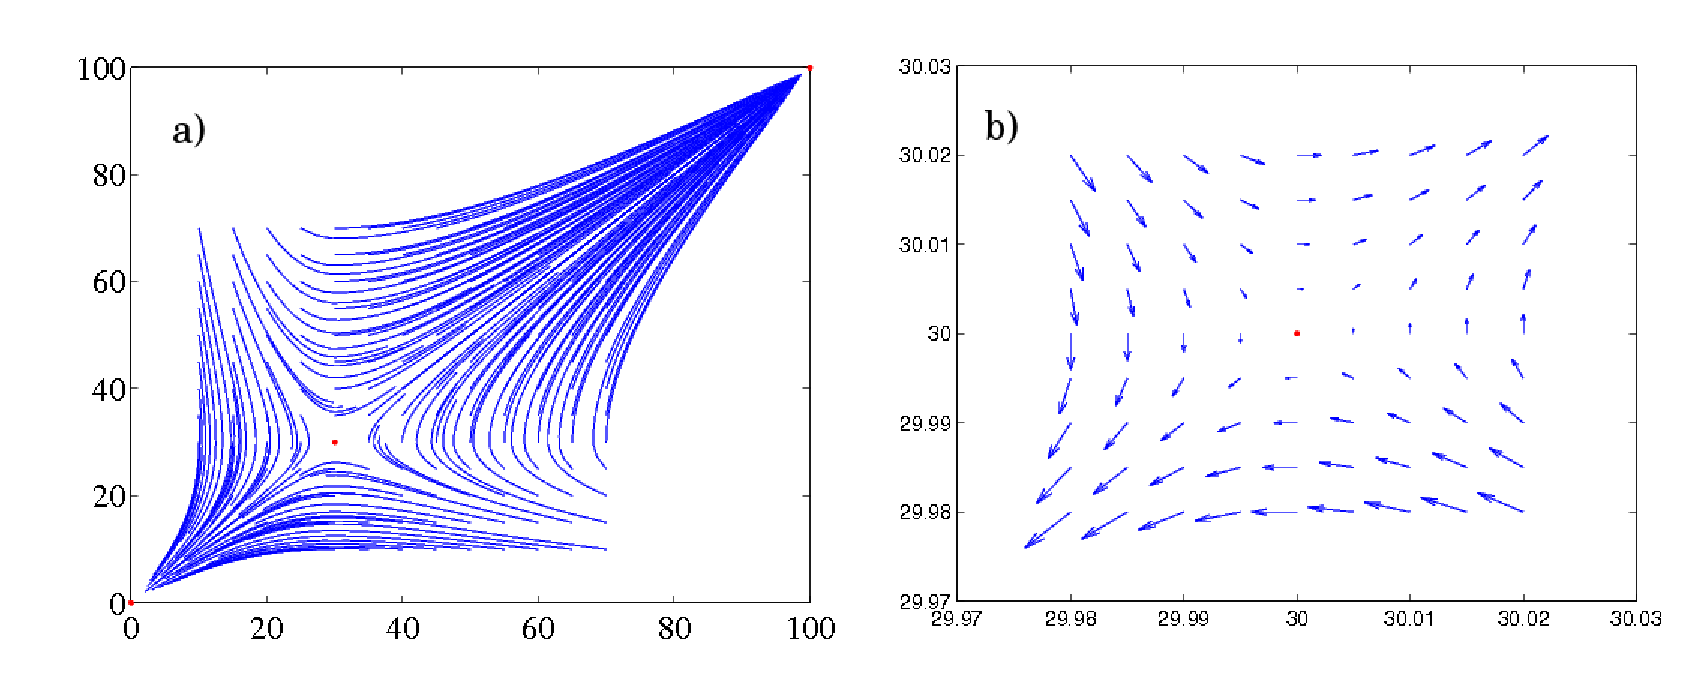
\includegraphics[scale = 0.5]{DINAMICA_solut_r9b03K100+flowdiagram.eps}
\caption {a) Soluciones del sistema \ref{eq:new_model} apara $r_1=r_2=-0.9$, $b_{12}=b_{21}=0.03$ y $K_1=K_2=100$. b) Diagrama de flujo en la vecindad del \textit{saddle point} en ($30,30$).}
\label{fig:stab1_phase}
\end{figure}

Este \textit{saddle point} marca la frontera entre la cuenca de atracción de los puntos fijos estables y, en consecuencia, controla la resistenca del sistema ante perturbaciones externas. Si está próximo a la destrucción completa ($N_1=0$,$N_2=0$), el sistema es más estable porque la cuenca de atracción de $(K_1,K_2)$ es más extensa. Sucede lo contrario cuando se localiza cerca del máximo vital, es decir, con ambas poblaciones tomando los valores máximos de sus capacidades de carga.

La figura \ref{fig:stab1_phase}a muestra las soluciones del sistema \ref{eq:new_model} para dos especies con mutualismo obligado ($r_1<0$ y $r_2<0$), e incio de las trayectorias en los puntos de la rejilla entre $10$ y $70$; la \ref{fig:stab1_phase}b es el diagrama de flujo en torno al \textit{saddle point} en ($30,30$). Cuanto mayor sea la intensidad del mutualismo, más próximo se encuentra este punto al origen.


\subsection{Generalización con $n$ especies}

Para una red con múltiples especies, hay que analizar el sistema de ecuaciones \ref{eq:modelo_optionI}. Los puntos fijos son, de nuevo, la extinción total ($N_i=0$, para todo $i$), el máximo vital con todas las especies en sus capacidades de carga respectivas ($N_i=K_i$, para todo $i$), y cualquier combinación de la solución trivial $N_{i}=0$ con las $N_{j}= K_{j}$, con la condición para las especies supervivientes:
\begin{equation}
\displaystyle r_{\rm{eff},j}^{\ast} = r_{j} + \sum_{l} b_{jl}\, K_{l} > 0 \\
\label{eq:condit_reff_K}
\end{equation}

\noindent done $l$ es el índice para todas las especies de la clase diferentes de $j$ que alcanzan la capacidad de carga en el punto fijo ($N_{l}=K_{l}$). El jacobiano para la extinción total es como la ecuación \ref{eq:Jacob00}, con las tasas vegetativas en la diagonal, y por tanto es una solución estable para mutualismo obligado ($r_i<0$ para todo $i$) e inestable en otro caso. Para poblaciones en máximos, el jacobiano es como en \ref{eq:JacobK1K2}
\begin{equation}
%\begin{align*}
\displaystyle
\mathbf{J}_{\left(N_i=K_i, N_j=K_j\right)}= \left(
  \begin{array}{ccc}
    -r_{\rm{eff},i} & \cdots & 0\\
    \vdots & \ddots & \vdots \\
    0 & \cdots & -r_{\rm{eff},j}
    \end{array} \right)
\stepcounter{equation}\tag{\theequation}\label{eq:GenJacobK1K2}
%\end{align*}
\end{equation}

Esta solución es estable porque todos los autovalores $\lambda_i=-r_{\rm{eff},i}^{\ast}$ son negativos (como en \ref{eq:condit_reff_K}). La estabilidad de las soluciones de las extinciones parciales para $N_k=0$ y $N_l=K_l$, con $k$ para las especies que se extinguen y $l$ para las que sobreviven, puede deducirse de las entradas genéricas del jacobiano:
\begin{align*}
\displaystyle &\frac{\partial f_i}{\partial N_i} = r_{\rm{eff},i}-2\left|r_{\rm{eff},i}\right| \frac{N_i}{K_i}\\
\displaystyle &\frac{\partial f_i}{\partial N_j} = N_i\,b_{ij}-sgn\left(r_{\rm{eff},i}\right)b_{ij}\frac{{N_i}^2}{K_j}
\stepcounter{equation}\tag{\theequation}\label{eq:partial_ij}
\end{align*}

\noindent El jacobiano es diagonal con los valores

\begin{equation}
%\begin{align*}
\displaystyle
\mathbf{J}_{\left(N_k=0,N_l=K_l\right)}= \left(
  \begin{array}{ccc}
    r_{\rm{eff},k} & \cdots & 0\\
    \vdots & \ddots & \vdots \\
    0 & \cdots & -r_{\rm{eff},l}
    \end{array} \right)
%\stepcounter{equation}\tag{\theequation}
\label{eq:Jacob0_iK_j}
%\end{align*}
\end{equation}

\noindent donde las $r_{\rm{eff},k}$ son positivas porque

\begin{equation}
%\begin{align*}
\displaystyle
\left.\frac{\partial f_k}{\partial N_k} \right|_{N_k=0} = r_k + \sum_{l}b_{kl}K_l\\
\label{eq:partial_N_0}
\end{equation}

\noindent y las $r_{\rm{eff},l}$ son negativas porque
\begin{equation}
%\begin{align*}
\displaystyle
\left.\frac{\partial f_l}{\partial N_l} \right|_{N_l=K_l} = r_{\rm{eff},l} - 2 \left| r_{\rm{eff},l} \right| \frac{K_l}{K_l} \\
\label{eq:partial_N_K}
\end{equation}
%\end{align*}

\noindent y $r_{\rm{eff},l}>0$.

Entonces, la condición para que la extinción parcial sea estable es $r_k<-\sum_{s}b_{ks}K_s$, esto es, la tasa intrínseca de crecimiento de las especies que se extinguen es más negativa que menos la contribución mutualista de las especies a las que se conecta y $r_l>-\sum_{s}b_{ls}K_s$, esto es, la tasa intrínseca de crecimiento de las especies supervivientes es mayor que menos la contribución mutualista de sus benefactoras.

Otros puntos fijos se obtienen de la condición $r_{\rm{eff},i}=0$, para todo $i$. Como se comentó en el caso de $1+1$ especies, la función valor absoluto no es diferenciable en $x=0$. Sin embargo, podemos definir las derivadas en la vecindad del punto (\ref{eq:deriv_reff_0}). Suponiendo que $r_{\rm{eff},i}>0$ los términos del jacobiano son:
\begin{align*}
\displaystyle
&\left.\frac{\partial f_i}{\partial N_i} \right|_{r_{\rm{eff},i}=0^{+}} =0\\
&\left.\frac{\partial f_i}{\partial N_j} \right|_{r_{\rm{eff},i}=0^{+}} =N_i\,b_{ij} \left( 1- \frac{N_i}{K_i} \right) \equiv J_{ij}>0
\stepcounter{equation}\tag{\theequation}
\label{eq:rmefi0}
%\end{equation}
\end{align*}

\noindent que es una matriz no negativa. Este punto fijo no es estable porque los autovalores no pueden ser simultáneamente negativos:
\begin{equation}
\displaystyle
  \sum_i \lambda_i = \rm{Tr} (\mathbf{J})
\end{equation}

Este es el punto intermedio de la solución, entre la extinción total y el máximo vital; si existe, es inestable.

\clearpage
\section{Modelo con saturación del beneficio}

La hipótesis de partida es que el mutualismo incrementa a tasa intrínseca de crecimiento de las especies. Esta suposición se basa en observaciones según las cuales la variación de la tasa de crecimiento de las poblaciones (o la fertilidad) tiene una alta correlación con la disponiblidad de recursos \cite{stenseth1998,krebs2002,rueness2003,tyler2008,jones2008}. En este contexto los recursos son las interacciones mutualistas. Supongamos que la comunidad está compuesta por $n_a$ especies de animales, con poblaciones $\{N_{i}^a\}$, y $n_p$ especies de plantas con poblaciones $\{N_{j}^p\}$. El beneficio mutualista entre las especies $i$  de una clase y $j$ de la otra se representa con el elemento $b_{ij}$ de la matriz de interacción. Debe tenerse en cuenta que las matrices no son necesariamente simétricas y que la intensidad del beneficio de la interacción no es la misma en ambos sentidos. Para una especie animal $i$, escribimos su tasa de crecimiento como
\begin{align}
r_{i} = r_{i}^{0} + \sum_{k=1}^{n_{p}} b_{ik}\, N^{p}_k
\label{eq:expr}
\end{align}
En esta expresión, $r_{i}^{0}$ es la tasa de crecimiento vegetativo. Para impedir un crecimiento ilimitado de dicha tasa, el efecto del mutualismo tiene que saturar en cierto punto.

Siguiendo la idea de Velhurst, proponemos un modelo en el que el término de fricción $\alpha_i$ depende también de la intensidad de la interacción mutualista. La traducción biológica de esta idea es que a partir de un determinado nivel el aumento de individuos de la especie mutualista no aporta beneficio adicional. Imaginemos una especie de polinizadores y una planta de la que obtienen alimento en forma de néctar. Si la población de plantas crece sin medida, llegará un momento en que los insectos no podrán libar todo el néctar producido. Para mantener el modelo simple, suponemos que el efecto del mutualismo sobre $\alpha$ es proporcional al beneficio. 
\begin{align}
\alpha_i = \alpha_{i}^{0}+ c_{i} \sum_{k=1}^{n_{p}} b_{ik}\, N^{p}_k 
\stepcounter{equation}\tag{\theequation}
\label{eq:alphavariable}
\end{align}
El término $c_{i}$ es el coeficiente de proporcionalidad. Las expresiones para las plantas son similares con el sumatorio sobre las especies de animales. Para simplificar la notación, eliminaremos los ceros de $\alpha_{i}^{0}$ y $r_{i}^{0}$ allí donde no haya confusión posible. Bajo estas suposiciones la dinámica del modelo propuesto está gobernada por el siguiente juego de ecuaciones:

\begin{theo} 
Modelo de dinámica mutualista con saturación del beneficio.
\begin{align*}
\frac{1}{N^{a}_{i}}\frac{dN^{a}_{i}}{dt} = r_{i}+ \sum_{k=1}^{n_{p}} b_{ik}\, N^{p}_k - \left( \alpha_{i}+ c_{i} \sum_{k=1}^{n_{p}} b_{ik}\, N^{p}_k \right) N^{a}_{i} \nonumber\\
\frac{1}{N^{p}_{j}}\frac{dN^{p}_{j}}{dt} = r_{j}+ \sum_{\ell=1}^{n_{a}} b_{j\ell}\, N^{a}_\ell - \left( \alpha_{j}+ c_{j} \sum_{\ell=1}^{n_{a}} b_{j\ell}\, N^{a}_\ell \right) N^{p}_{j}
\stepcounter{equation}\tag{\theequation}\label{eq:DINAMICA_modeloralphaconmut}
\end{align*}
\end{theo}


Las expresiones en el lado derecho de las igualdades se pueden interpretar como \textit{tasas de crecimiento efectivas}. 

\begin{theo} 
Tasa de crecimiemto efectiva de la especie animal $i$.
\begin{equation}
r_{eff,i} = r_{i} + \sum_{k=1}^{n_{p}} b_{ik}\, N^{p}_k - \left( \alpha_{i}+ c_{i} \sum_{k=1}^{n_{p}} b_{ik}\, N^{p}_k \right) N^{a}_{i}
\label{eq:DINAMICA_effrate}
\end{equation}
\end{theo}

Las tasas efectivas de las especies de plantas se definen de forma similar sustituyendo $a$ por $p$. Las \textit{capacidades de carga} del sistema son los puntos fijos distintos de cero de las ecuaciones \ref{eq:DINAMICA_modeloralphaconmut}. Es sencillo ver que en ausencia de mutualismo $K_i = r_i/\alpha_i$ para la especie $i$. Por el contrario, en presencia de mutualismo muy intenso, $K_i$ tiende a $1/c_{i}$. El papel de la constante de proporcionalidad $c_i$ es, por tanto, limitar la población máxima de la especie $i$ cuando $c_{i} \sum_{k=1}^{n_p} b_{ik} \, N^p_{k} \gg \alpha_{i}$. 

Consideramos que este modelo podría resultar también válido para otro tipo de interacciones ecológicas en las que todos los términos $b_{ik}$ son positivos, como el comensalismo ($b_{ij}=0, b_{ji}>0)$ y el antagonismo ($b_{mn}>0,b_{nm}<0$). 

\subsection{Análisis de estabilidad para dos especies}

Por simplicidad empezamos con la comunidad mutualista más sencilla, formada por una especie de cada clase, para la cual podemos obtener resultados analíticos completos. Sea la planta la especie que designamos con el índice $1$ y el animal la representada como $2$. El modelo \ref{eq:DINAMICA_modeloralphaconmut} se reduce a:

\begin{align}
\frac{dN^p_{1}}{dt} = \left( r_{1}+ b_{12}\, N^a_{2}\right) \ N^p_{1} - \left(\alpha_{1}+ c_{1} \, b_{12} \, N^a_{2} \right) {N^p_{1}}^2 ,\nonumber\\ 
\frac{dN^a_{2}}{dt} = \left( r_{2}+ b_{21}\, N^p_{1}\right)N^a_{2} - \left(\alpha_{2}+ c_{2} \, b_{21}\, N^p_{1} \right) {N^a_{2}}^2 .
\stepcounter{equation}\tag{\theequation}\label{eq:DINAMICA_dos_especies}
\end{align}

La figura \ref{DINAMICA_diagram} representa varios diagramas de flujo del sistema con distintas configuraciones de los parámetros.

\begin{figure*}
\centering
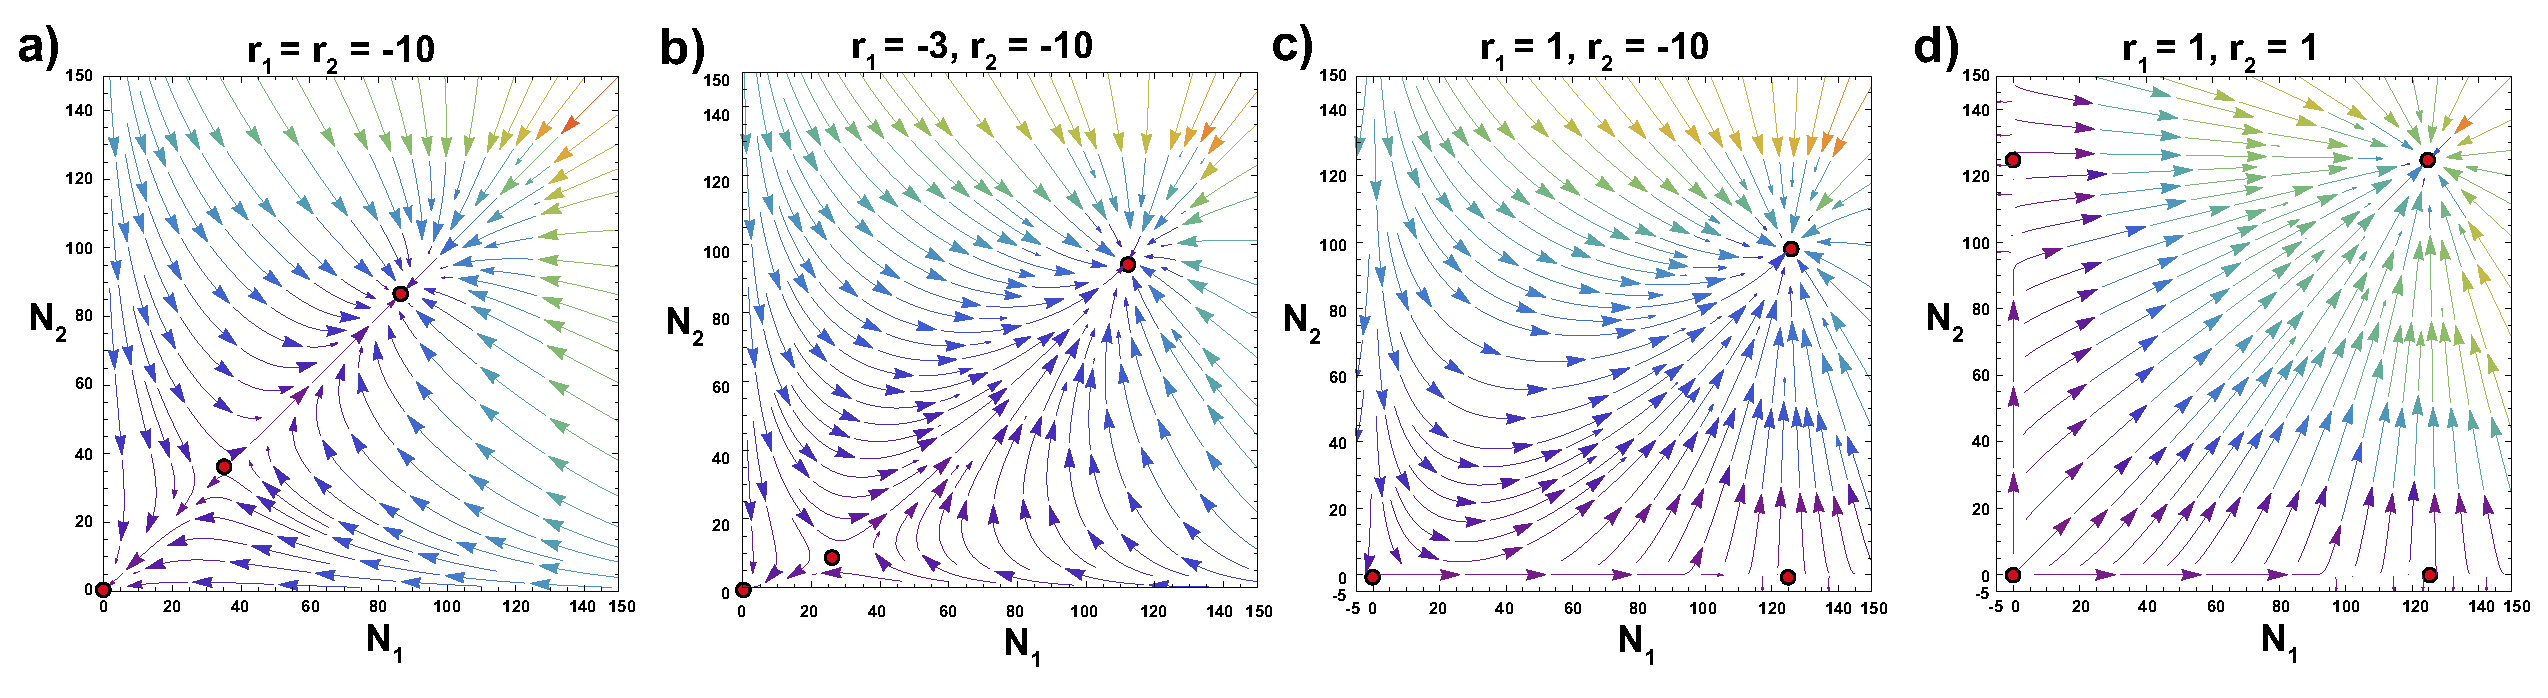
\includegraphics[scale=0.35]{DINAMICA_Figure1h.eps}
\caption {Diagrama de flujo de la dinámica de una comunidad de dos especies según el modelo de ecuaciones \ref{eq:DINAMICA_dos_especies}. Los puntos fijos se han resaltado como círculos de color rojo. El color de las flechas indica la intensidad del flujo. Las cuatro imágenes corresponden a diferentes valores para las tasas intrínsecas de crecimiento. El resto de parámetros mantiene los mismos valores en los cuatro casos: $\alpha_1 = \alpha_2 = 0.008$, $b_{12} = b_{21} = 0.4$ y $c_1 = c_2 = 0.008$. El mutualismo es obligatorio en a) y b), aunque en diferente grado en el segundo diagrama. Es obligatorio para la especie 2 en c), mientras que la especie 1 podría sobrevivir sin la 2. En d) el mutualismo es facultativo para ambas especies.}
\label{DINAMICA_diagram}
\end{figure*}

Para encontrar los puntos fijos del sistema hacemos $\frac{dN^p_{1}}{dt} = \frac{dN^a_{2}}{dt} = 0$. El primero y más obvio, corresponde a la extinción total $({N^p_{1}}^*,{N^a_{2}}^*) = (0,0)$ con independencia del valor de los parámetros. Si cualquiera de las tasas de crecimiento intrínseco $r_1$, $r_2$ es positiva, entonces encontramos puntos fijos adicionales que aparecen por extinciones parciales. La dinámica de la población superviviente, con $r$ positivo, sigue en tal caso una ecuación logística como se deduce de la expresión \ref{eq:DINAMICA_dos_especies}. En consecuencia, su población tenderá a la capacidad de carga sin mutualismo ya sea $K_1 = r_1/\alpha_1$ o $K_2 = r_2/\alpha_2$. 

Las extinciones se producen en los puntos fijos $(K_1,0)$ ó $(0,K_2)$, o en ambos si el mutualismo es facultativo solo para la especie $1$ ($r_1 >0$), solo para la especie dos $2$ ($r_2 >0$) (figura \ref{DINAMICA_diagram}c) o para las dos ($r_1>0$ y $r_2 >0$) (figura \ref{DINAMICA_diagram}d). 

Además de los puntos fijos correspondientes a extinciones, aparecen otros no triviales cuando se cumple la condición $r_{eff,i} = r_{eff,j} = 0$. Para dichos puntos se verifica que: 
\begin{align}
{N^p_{1}}^* = \frac{ r_{1}+ b_{12} \, {N^a_{2}}^* }{\alpha_{1}+ c_{1}\, b_{12}\, {N^a_{2}}^* } , \nonumber\\ 
{N^a_{2}}^* = \frac{ r_{2}+ b_{21}\, {N^p_{1}}^* }{\alpha_{2}+ c_{2} \, b_{21}\, {N^p_{1}}^* } .
\label{eq:DINAMICA_puntosfijos}
\end{align}

Sustituyendo la expresión de ${N^{a}_2}^*$ en la ecuación superior, encontramos que ${N^p_1}^*$ es la solución de una ecuación cuadrática en los puntos fijos: 
\begin{equation}
A\, {{N^p_1}^*}^2 + B \, {N^p_1}^* + C=0 ,
\label{eq:DINAMICA_quadra}
\end{equation}

Los coeficientes $A$, $B$ y $C$ valen:

\begin{align}
\displaystyle A &= c_{2}\, b_{21}\, \alpha_{1}+c_{1}\, b_{12}\, b_{21} , \nonumber \\
\displaystyle B &= \alpha_{1}\, \alpha_{2}+ c_{1}\, b_{12}\, r_{2} - c_{2}\, b_{21}\, r_{1} - b_{12}\, b_{21} ,\nonumber\\
\displaystyle C &= - r _{1}\, \alpha_{2} - b_{12}\, r_{2} .
\label{eq:DINAMICA_puntos_n1}
\end{align}

Los puntos fijos para ${N^a_2}^*$ se encuentran sustituyendo ${N^p_1}^*$ en la expresión inferior de la ecuación \ref{eq:DINAMICA_puntosfijos}. Aparecen distintos escenarios dependiendo de las soluciones de la ecuación \ref{eq:DINAMICA_quadra}:

\begin{enumerate}
\item Ambas raíces complejas. No hay puntos fijos que no supongan extinciones.
\item Una sola raíz real. Es un punto de bifurcación de la dinámica del sistema. Las soluciones son reales pero degeneradas. En este caso existe un único punto fijo aparte de los de extinción. El estado final del sistema depende de la estabilidad de dicho punto. Sin embargo, lo más probable es que las poblaciones terminen extinguiéndose.
\item Dos raíces reales. La situación es similar a la representada en la imagen de la izquierda de la figura \ref{DINAMICA_diagram}. Hay dos puntos fijos no triviales, típicamente uno estable y un \textit{saddle point} sobre la divisoria de las dos cuencas de atracción. La posición de este segundo punto depende de la extensión de la cuenca de extinción y, por tanto, de la resistencia del sistema ante perturbaciones externas. Lo denominamos \textit{mínimo vital} y su valor lo representamos como$({N_{1}^{p}}^\bullet,{N_{2}^{a}}^\bullet)$.
\end{enumerate}

Para estudiar la estabilidad lineal de los puntos fijos, expandimos las ecuaciones \ref{eq:DINAMICA_dos_especies} en serie de Taylor en torno a ellos y calculamos el jacobiano del sistema (ver los detalles en el anexo \ref{DINAMICA_ANEXO_estabilidad}). Si los autovalores son negativos, el punto fijo es estable. En caso contrario, puede ser un \textit{saddle} si uno es positivo y otro negativo o inestable si ambos son positivos. Comenzando por la extinción total, el jacobiano puede escribirse como: 
\begin{equation}
J = \left(
\begin{array}{ll}
r_{1}   & 0 \\
0 & r_{2} 
\end{array}
\right) \stepcounter{equation}\tag{\theequation}\label{eq:J00}
\end{equation}

Lo autovalores son $\lambda_{1,2} = r_{1,2}$, lo que indica que el punto de extinción es linealmente estable bajo la hipótesis de que $r_{1}<0$ y $r_{2}<0$; es decir, ambas especies dependen del mutualismo para sobrevivir. La extinción total tiene una cuenca de atracción para los distintos valores de las poblaciones. Si el sistema entra en ella, el único destino posible es la destrucción de la comunidad.

Por el contrario, si el mutualismo es facultativo para una o ambas especies, la extinción total se convierte en un \textit{saddle} o en un punto inestable. No obstante, pueden aparecer otros dos puntos fijos correspondientes a extinciones parciales. En estas circunstancias, la condición de estabilidad para $(r_1/\alpha_1, 0)$ es que $r_{1}>0$ y $r_{2}<-b_{21}\, r_{1}/\alpha_{1}$. Análogamente, $(r_1/\alpha_1, 0)$ es estable si y solo si  $r_{2}>0$ y $r_{1}<-b_{12}\, r_{2}/\alpha_{2}$.
El mismo análisis para los restantes casos de puntos fijos no triviales se traduce en el jacobiano:

\begin{equation}
J = \left(
\begin{array}{ll}
- {N^{p}_{1}}^* \, (\alpha_{1}+ c_{1}\, b_{12} \, {N^a_2}^* )  & {N_{1}^{p}}^* \, b_{12} \, (1 - c_{1}\, {N_{1}^{p}}^* ) \\
{N_{2}^{a}}^* \, b_{21}\, (1 - c_{2}\, {N_{2}^{a}}^* ) & - {N_{2}^{a}}^* \, (\alpha_{2}+ c_{2}\,b_{21}\,{N_{1}^{p}}^* )
\end{array}
\right)\stepcounter{equation}\tag{\theequation}\label{eq:J}
\end{equation}
Como los parámetros $c_{1}$ y $c_2$ son siempre positivos (recordemos que son el inverso del límite de población en presencia de un mutualismo muy intenso), y que todos los términos de $J$ tienen el signo mostrado en la ecuación \ref{eq:J}. Los elementos de la diagonal son negativos, mientras que el resto son siempre positivos (una configuración similar del jacobiano para modelos mutualistas aparece en \cite{goh1979}. Esto implica que los autovalores de $J$ son ambos reales y pueden ser los dos negativos (\textit{puntos fijos estables}) o uno positivo y otro negativo (\textit{saddle}). La condición para la existencia de este último es que el determinante del jacobiano en el \textit{mínimo vital} sea negativo, $J_{11} \, J_{22} < J_{12}\, J_{21}$, que en función de ${N_{1}^{p}}^\bullet$ y ${N_{2}^{a}}^\bullet$ significa que:

\begin{equation}
1-c_{1}\, {N_{1}^{p}}^\bullet - c_{2}\, {N_{2}^{a}}^\bullet > 0 .
\end{equation}

Todos estos resultados para dos especies indican que el modelo presenta una dinámica muy rica. Pese a ello, es los suficientemente simple para entender bien los diferentes regímenes y donde se localizan en el espacio de configuración de los parámetros. En este sentido, soluciona algunas de las limitaciones del modelo tipo II. Por ejemplo, encontrar una configuración para dos especies como la que aparece en la figura \ref{DINAMICA_typeII} requiere un esfuerzo considerable de afinamiento de los parámetros. Esta configuración con dos atractores y una divisoria nítida es ideal para estudiar fenómenos como la resistencia de la red, la capacidad de soportar una alta biodiversidad o la evolución de las interacciones de la red \cite{bastolla2009, suweis2013emergence}. Este régimen aparece de forma natural en el modelo propuesto, como se ve en la figura \ref{DINAMICA_diagram}, sin la necesidad de un complejo proceso de afinamiento. Además, como veremos en los siguientes apartados, una configuración equivalente con un atractor de extinción, otro con poblaciones finitas y una clara divisoria, aparece al extender el estudio a redes con muchas más
especies.

\begin{figure}
\centering
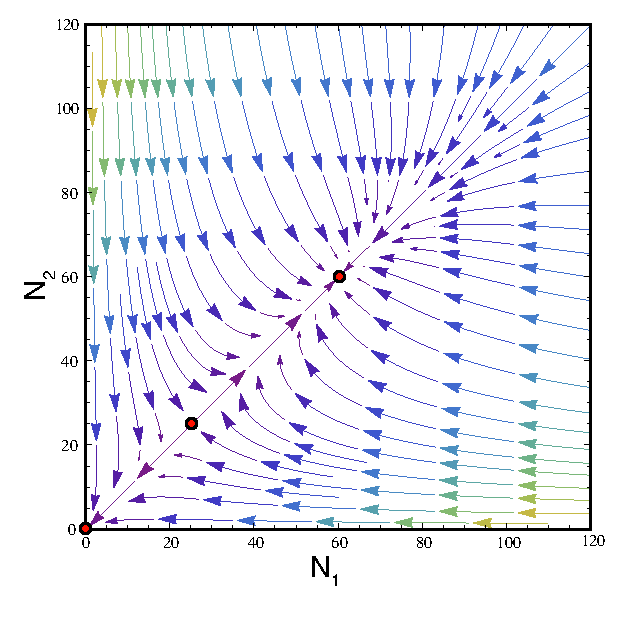
\includegraphics[scale=0.66]{DINAMICA_Figure2.eps}
\caption {Diagrama de flujo para la dinámica de ecuaciones de tipo II \ref{DINAMICA_typeII}. Encontrar esta configuración requirió un ajuste de parámetros laborioso. Los valores empleados en este ejemplo son $r_1 = r_2 = -0.1$, $\alpha_1 = \alpha_2 = 0.001$, $a = 0.066$, $b = 0.2$ y $T_H = 1$.}
\label{DINAMICA_typeII}
\end{figure}

\subsection{La divisoria de la vida}
\label{watershed}

Llamaremos \textit{divisoria de la vida} al límite que separa las trayectorias que evolucionan hacia la capacidad máxima de población del sistema de las que terminan en su destrucción. En la imagen izquierda de la figura \ref{DINAMICA_diagram} es la frontera entre las cuencas de atracción del punto de extinción en el origen y del máximo estable de poblaciones. La divisoria incluye al \textit{saddle} no trivial $({N_1^p}^\bullet,{N_2^a}^\bullet)$, la combinación mínima de poblaciones que garantiza la supervivencia. Su ubicación en el espacio de fases es importante porque determina la posición base de dicha curva y en consecuencia la fragilidad del sistema, que se expresa como la relación de áreas entre las dos cuencas de atracción. La distancia de este punto al máximo de poblaciones indica la resistencia ante perturbaciones externas. Si es muy pequeña, una ligera disminución del número de individuos, provocada por enfermedades, sequías o siniestros de cualquier naturaleza puede llevar al sistema a la cuenca de destrucción. Por el contrario, si esta distancia es grande, la comunidad podrá recobrarse de estos eventos y crecer de nuevo hacia el máximo. Como los ciclos naturales suelen ser cíclicos, la combinación de poblaciones se moverá de manera habitual entre estos puntos, y un amplio rango dinámico facilita la permanencia en el tiempo. 

Para el sistema mínimo, de dos especies, las principales características de la divisoria se pueden encontrar analíticamente. Los puntos de la curva se corresponden a los pares de poblaciones $({N_1^p},{N_2^a})$ para los cuales la dinámica del sistema evoluciona exactamente sobre la curva y termina en el punto fijo $({N_1^p}^\bullet,{N_2^a}^\bullet)$. Sabemos que es un punto inestable y que la menor perturbación conducirá hacia uno u otro lado de la divisoria, pero conocer la expresión analítica de la curva supone un gran avance.  

Por definición, en $({N_1^p}^\bullet,{N_2^a}^\bullet)$ las tasas efectivas de crecimiento son nulas. Para llegar a este punto desde cualquier otro de la divisoria, las tasas de ambas especies deben ser de signo contrario y evolucionar en el tiempo de forma similar. Si las dos fueran del mismo signo, las trayectorias irían hacia la extinción (negativo) o hacia el máximo vital (positivo). 

Supongamos que el sistema se aproxima a $({N_1^p}^\bullet,{N_2^a}^\bullet)$, desde una posición inicial $({N_1^p}^0,{N_2^a}^0)$ perteneciente a la divisoria. Las tasas efectivas de crecimiento son:

\begin{align}
r_{eff,1}  = & \, A \, e^{-\gamma\, t} ,\nonumber\\  
r_{eff,2}  = & -B\, e^{-\gamma\, t} , 
\label{eq:coeffsreffs}
\end{align}
donde $A$, $B$ y $\gamma$ son constantes desconocidas por el momento. El sistema de ecuaciones \ref{eq:DINAMICA_dos_especies} se convierte en el siguiente:
\begin{align}
\frac{dN^p_{1}}{dt} & = N^p_{1} \, A \, e^{-\gamma \, t} , \nonumber \\
\frac{dN^a_{2}}{dt} & = -N^a_{2}\, B \, e^{-\gamma \, t} .
\label{eq:coeffsreffs_2}
\end{align}

Integrando ambas ecuaciones entre $t = 0$ e infinito  encontramos que:

\begin{align}
 \ln \left(\frac{{N_1^p}^\bullet}{{N_{1}^p}^0} \right) & = \frac{A}{\gamma} , \nonumber\\ 
 \ln \left(\frac{{N_2^a}^\bullet}{{N_{2}^a}^0} \right) & = - \frac{B}{\gamma} .
\label{eq:coeffsreffs_3}
\end{align}

Como el valor de $\gamma$ tiene que ser el mismo para ambas expresiones, obtenemos la condición que tienen que cumplir $({N_1^p}^0,{N_2^a}^0)$ para pertenecer a la divisoria:

\begin{align}
\frac{1}{B} \ln \left(\frac{{N_{2}^a}^\bullet}{{N_{2}^a}^0} \right) + \frac{1}{A} \ln \left(\frac{{N_1^p}^\bullet}{{N_1^p}^0} \right) = 0 ,
\label{eq:coeffsreffs_4}
\end{align}

Esto significa que la expresión funcional de la divisoria es una ley de potencia.

\begin{align}
{N_2^a}^0 = C\, ({N_1^p}^0)^\frac{-B}{A}. 
\label{eq:powerlaw}
\end{align}
Podemos despejar la constante $C$ teniendo en cuenta que la divisoria incluye el punto fijo $({N_1^p}^\bullet,{N_2^a}^\bullet)$, así que podemos escribir:

\begin{align}
C = {N_2^a}^\bullet / ({N_1^p}^\bullet)^\frac{-B}{A} .
\end{align}

Para encontrar el valor del exponente fraccionario $\frac{B}{A}$, debemos volver a la definición de las tasas de crecimiento efectivas $r_{eff,1}$ y $r_{eff,2}$. De acuerdo con las ecuaciones \eqref{eq:coeffsreffs}, en $t=0$ tenemos que:
 
\begin{align}
A = & \, r_{1}+ b_{12}\, {N_2^a}^0 - (\alpha_{1}+ c_{1} \, b_{12}\, {N_{2}^a}^0) \, {N_1^p}^0 , \nonumber\\
-B = &\, r_{2} + b_{21} \, {N_{1}^p}^0-(\alpha_{2}+ c_{2}\,  b_{21}\, {N_{1}^p}^0)\,  {N_{2}^a}^0 .
\label{eq:reffs_2especies}
\end{align}

Si sabemos que nuestro punto inicial era parte de la divisoria, podemos obtener el valor del exponente dividiendo estas expresiones.

Alternativamente, si necesitamos encontrar otros puntos de la divisoria que no sean $({N_1^p}^\bullet,{N_2^a}^\bullet)$, podemos dividir las expresiones anteriores y, usando la ecuación \ref{eq:coeffsreffs_3}, llegar a la siguiente ecuación implícita:

\begin{align}
\frac {\ln \left( \frac{{N_2^a}^\bullet}{{N_2^a}^0} \right)}{\ln \left( \frac{{N_1^p}^\bullet}{{N_1^p}^0} \right)} = \frac{( r_{2}+ b_{21}\, {N_1^p}^0) - (\alpha_{2}+ c_{2} \,  b_{21}\, {N_1^p}^0 ) \, {N_1^p}^0}{( r_{1}+ b_{12}\, {N_2^a}^0) - (\alpha_{1}+ c_{1} \, b_{12}\, {N_2^a}^0 ) \, {N_2^a}^0 } .
\label{eq:implicita_watershed}
\end{align}

Resolviendo esta ecuación de forma numérica podemos encontrar cualquier punto de la divisoria, y con ello obtenemos el valor del exponente $\frac{B}{A}$. 

La figura \ref{fig:powerlaw} muestra un ejemplo concreto de divisoria, y una comparación entre la curva definida por el sistema \ref{eq:powerlaw} y la ecuación implícita \ref{eq:implicita_watershed}. Ambas se han resuelto por integración numérica. Los puntos rojos se han encontrado haciendo un barrido del espacio de parámetros en una aproximación de \textit{fuerza bruta}, determinando el límite entre extinción y evolución hacia la capacidad máxima. La línea gris continua es la ley de potencia que se obtiene resolviendo las ecuaciones \ref{eq:powerlaw} y \ref{eq:implicita_watershed}

\begin{figure}[ht!]
\centering
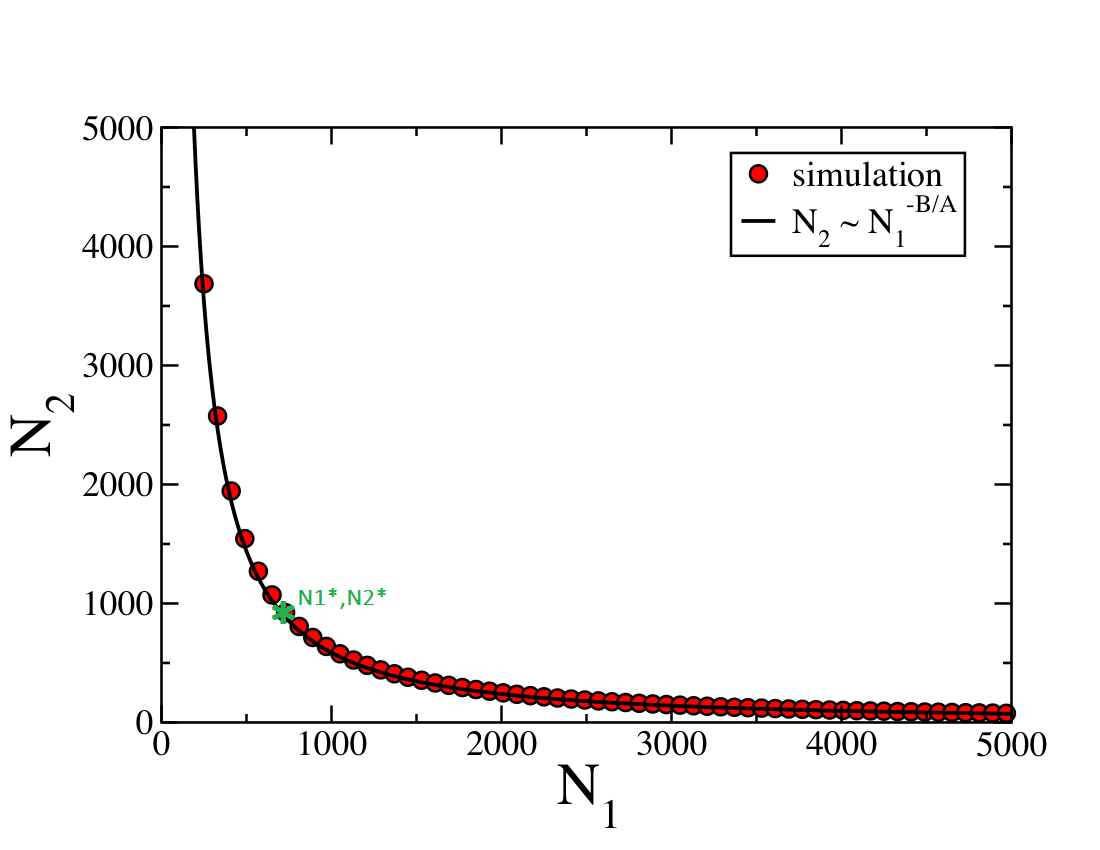
\includegraphics[scale=0.5]{DINAMICA_Figure3.png}
\caption {Divisoria de la vida para dos especies. En este caso, $\frac{B}{A}=1.2944,~{N_1^p}^\bullet=692,~{N_2^a}^\bullet=989,~b_{12}=0.000041850,~c_{1}=0.00004,~\alpha_{1}=~0.000035,~r_1=-0.016,~b_{21}=0.00008750,~c_{2}=0.0001,~\alpha_{2}=0.000035,~r_2 =-0.02$.}
\label{fig:powerlaw}
\end{figure}

\subsection{Generalización con $n$ especies}
 
La generalización del análisis de establidad para un número cualquiera de especies es simple. Los puntos fijos del sistema \ref{eq:DINAMICA_modeloralphaconmut} incluyen la solución trivial de destrucción del sistema $(N_{i}^p,\cdots, N_{j}^a) = (0, \cdots,0)$, los puntos de extinción parcial cuando el mutualismo es facultativo para algunas especies y los puntos fijos no triviales $({N^{a}_{i}}^*,\cdots,{N^{p}_{j}}^*)$ en los que las tasas de crecimiento efectivas son nulas:
\begin{align}
r^{*}_{eff,i}  = (r_{i}+ \sum_{k=1}^{n_{p}}\,  b_{ik}\, {N^p_{k}}^*)- (\alpha_{i}+c_{i}\, \sum_{k=1}^{n_{p}} b_{ik}\, {N^{p}_k}^* )\, {N^{a}_{i}}^* = 0 \nonumber ,\\
r^{*}_{eff,j}  = (r_{j}+ \sum_{\ell=1}^{n_{a}} b_{j\ell}\, {N^{a}_{\ell}}^*)- (\alpha_{j}+c_{j}\, \sum_{\ell=1}^{n_{a}} b_{j\ell}\, {N^{a}_\ell}^* )\, {N^{p}_{j}}^* 
=0 ,
\label{eq:effrate2}
\end{align}
Estas son las expresiones para animales y plantas. Se puede reescribir el sistema como:

\begin{align}  
{N^{a}_{i}}^* = \frac{r_{i}+\sum_{k=1}^{n_{p}}b_{ik}\, {N^{p}_{k}}^*}{\alpha_{i}+c_{i}\,\sum_{k=1}^{n_{p}}{b_{ik}N^{p}_{k}}^*} = 
  \frac{r_{i}+r_{i}^{mut}}{\alpha_{i}+c_{i}\, r_{i}^{mut}} = 
  \frac{r_{i}^{*+}}{r_{i}^{*-}} \nonumber\\
{N^{p}_{j}}^*=\frac{r_{j}+\sum_{\ell=1}^{n_{a}}b_{j\ell}\, {N^{a}_{\ell}}^*}{\alpha_{j}+c_{j}\,\sum_{\ell=1}^{n_{a}}{b_{j\ell}N^{a}_{\ell}}^*} =
  \frac{r_{j}+r_{j}^{mut}}{\alpha_{j}+c_{j}r_{j}^{mut}} =
  \frac{r_{j}^{*+}}{r_{j}^{*-}}
\end{align}

Donde las tasas $r_{i}^{mut}$ representan el efecto del mutualismo sobre la especie $i$, mientras que las tasas $r^{*+}$ son las que incrementan el crecimento de la población y las $r^{*-}$ las que lo disminuyen vía competición intra especies. 

Las ecuaciones  \ref{eq:DINAMICA_modeloralphaconmut} se pueden linealizar en torno a los puntos fijos. El jacobiano tiene el mismo aspecto que el correspondiente al sistema mínimo de dos especies (ecuación \eqref{eq:J}), con términos negativos en la diagonal de la matriz y positivos o nulos fuera de ella. Para los puntos fijos no triviales se pueden escribir como (véase el Anexo \ref{DINAMICA_ANEXO_estabilidad}):
\begin{align}
\displaystyle & J_{ii}= - {N^{a}_{i}}^* \left(\alpha_{i} + c_{i} \,  \sum_{k=1}^{n_{p}} b_{ik} {N^{p}_{k}}^* \right) \nonumber\\
\displaystyle & J_{jj}= - {N^{p}_{j}}^* \left(\alpha_{j} + c_{j} \, \sum_{\ell=1}^{n_{a}} b_{j\ell}\, {N^{a}_{\ell}}^*\right)
\label{eq:Jii}
\end{align}
Los coeficientes fuera de la diagonal son:
\begin{align}
\displaystyle & J_{ij}={N^{a}_{i}}^* \, b_{ij}\, \left( 1-c_{i}\, {N^{a}_{i}}^*\right) 
\label{eq:Jij1}
\end{align}
para la interacción entre una especie animal $i$ y una planta $j$, y 
\begin{align}
\displaystyle & J_{ji}={N^{p}_{j}}^* \, b_{ji}\, \left( 1-c_{j}\, {N^{p}_{j}}^*\right)
\label{eq:Jij2}
\end{align}
para la correspondiente al sentido planta $j$ y animal $i$. Dada la invariancia de la traza de la matriz bajo un cambio de la base vectorial, la suma de autovalores de la matriz debe satisfacer la siguiente relación:
\begin{equation}
  \sum_{k}^{n_{a}+n_{p}} \lambda_{k}= - \left(\sum_{k}^{n_{a}+n_{p}} |J_{kk}| \right)
  \stepcounter{equation}\tag{\theequation}\label{eq:sum_lambdas2}
\end{equation}
La traza es negativa, lo que significa que si hay autovalores positivos o nulos su efecto debe compensarse por otros autovalores negativos. En consecuencia, los puntos fijos no triviales pueden ser estables si todos los autovalores son negativos, o \textit{saddle} si al menos uno de ellos en positivo. No es posible que sean puramente inestables.

Otro extremo que hay que investigar es lo que sucede en caso de extinciones parciales. El efecto de la desaparición de algunas especies es reducir las dimensiones del sistema de ecuaciones \ref{eq:DINAMICA_modeloralphaconmut}. Para hacerlo más simple, asumamos, por ejemplo, que la especie animal $e$ se extingue. Esto significa que los posibles puntos fijos del sistema deben incluir ahora ${N_e^a}^* = 0$. El colapso de $e$ puede provocar la extinción de algunas especies de plantas que se alimentaban con su polen, frutos o semillas, dependiendo del tipo de red. Estas extinciones pueden, a su vez, desencadenar la desaparición de especies animales que dependían de dichas plantas para su ciclo reproductivo. Este encadenamiento catastrófico es lo que se conoce como extinción en cascada. Aunque el fenómeno que produce la primera extinción sea externo y afecte a una sola especie, todas las demás se ven afectadas porque su dinámica está enlazada por el sistema de ecuaciones completo. Los nuevos puntos fijos no triviales se corresponden con los de extinción parcial del sistema original. La estabilidad de dichos puntos puede cambiar de manera sustancial con esta alteración de las condiciones. Los términos del jacobiano de las especies desaparecidas se convierten en $J_{ee} = r_e + \sum_{k =1}^{n_p }b_{ek}\,{N_k^p}^*$ en la diagonal y $J_{ej} = 0$ fuera de ella. Estos términos dejan de contribuir a los autovalores relevantes para la estabilidad del sistema. El resto de coeficientes del jacobiano se obtienen de las ecuaciones \ref{eq:Jii}, \ref{eq:Jij1}, y \ref{eq:Jij2} adaptadas a las especies supervivientes. Esto implica que los sumatorios de las ecuaciones \ref{eq:Jii} ya no incluyen todas las especies y que los términos de la diagonal pueden estar más próximos a cero. La establidad de los nuevos puntos fijos puede variar dependiendo de los parámetros de las ecuaciones del modelo de dinámica de poblaciones de las especies supervivientes. En realidad, dependiendo de la configuración resultante de la comunidad reducida, el sistema puede ser más robusto ante extinciones parciales que antes. Esto puede explicar por qué las comunidades mutualistas adoptan configuraciones fuertemente anidadas, son el resultado por prueba y error en el tiempo de extinciones parciales y de la llegada de nuevas especies que alteran su dinámica.   

\section{Material y métodos}

\subsection{Integración de las ecuaciones}
\label{DINAMINCA_NumSim}

Los modelos de población manejan cantidades discretas y la simulación es una herramienta potente para manejar la dinámica y el comportamiento estocástico. La elección de un método específico de simulación depende de su precisión y eficacia computacional y a veces representa un desafío.

Por ejemplo, los modelos discretos de Markov se han utilizado con frecuencia para este tipo de simulaciones, pero esta estrategia tiene desventajas comparada con la simulación estocática discreta, ya sea basada en la distribución de Poisson o en la binomial. Para los modelos de Markov de dimensiones moderadas, el número de estados puede ser muy grande, mientras que las simulaciones basadas en Poisson o binomial, con su manejo de variables de estado agregadas son mucho más rápidas  \cite{gustafsson2007bringing, balcan2009multiscale}.

Hemos elegido la simulación binomial para resolver las ecuaciones de ambos modelos. Esta técnica es una extensión de la simulación de sistemas continuos y una opción razonable cuando el resultado del proceso aleatorio tiene solo dos posibles valores. Por ejemplo, la supervivencia en un intervalo finito de tiempo es un ensayo de Bernoulli, el individuo sobrevive o no. La reproducción también puede modelarse adecuadamente como un ensayo de Bernouilli si el intervalo de simulación es pequeño. 

Para una especie con una tasa intrínseca de crecimiento $r$, podemos suponer que la probabilidad de reproducción en un intervalo $\Delta T$ sigue una distribución exponencial de valor medio $1/r$. Así, la probabilidad de reproducción es:
\begin{equation}
\label{eq:probbreeding}
P = \int_0^{\Delta T} \! re^{-r\, t}  \, dt = 1 - e^{-r\, \Delta T}
\end{equation}
En particular, una población de $N$ individos en el instante $t$, con crecimiento exponencial puro, será en $t+\Delta T$:
\begin{equation}
N(t+\Delta T)=N(t) + sgn \left(r \right) Binomial \left( N(t),P \right)
\end{equation}
\noindent El sistema de ecuaciones toma la forma estocástica siguiente:
\begin{equation}
\begin{split}
N^{a}_{j}(t+\Delta T)=N^{a}_{j}(t) + sgn \left(\hat{r}^{a}_{eff,j} \right) Binomial \left( N^{a}_{j}(t),P^{a}_{j}\right)\\
N^{p}_{l}(t+\Delta T)=N^{p}_{l}(t) + sgn \left(\hat{r}^{p}_{eff,l} \right) Binomial \left(N^{p}_{l}(t),P^{p}_{l} \right)
\end{split}
\end{equation}
\noindent donde $\hat{r}^{a}_{eff,j}$ es la tasa de crecimiento efectiva de la especie $j$ de la clase $a$ durante el periodo de simulación, y $P^{a}_{j}, P^{p}_{l}$ , las probabilidades de crecimiento según la ecuación \ref{eq:probbreeding}. En particular, si se trabaja con intervalos de un día, como en nuestros experimentos:
\begin{equation}
\hat{r}_{eff} = (1+r_{eff})^{1/365}-1
\end{equation}

La simulación estocástica tiene una ventaja adicional de gran interés. Las perturbaciones externas se modelan como variaciones temporales de la tasa efectiva de reproducción, restando el efecto del siniestro. Computacionalmente es muy sencillo llevar a cabo esta modificación; si, por el contrario, se resuelven numéricamente las ecuaciones diferenciales, hay que cambiar las condiciones iniciales para cada nueva perturbación y garantizar la continuidad en dichos puntos.

\subsection{Software}
Se ha desarrollado un simulador numérico (\textit{SIGMUND)} que es el que ha permitido llevar a cabo los experimentos (ver Apéncide \ref{APP_SIGMUNDMAN}). El lenguaje utilizado ha sido \texttt{Python}, con los paquetes \texttt{NumPy} y \texttt{SciPy} para la parte de cálculo, \texttt{PyQt} para construir una interfaz de usuario interactiva y \texttt{Matplotlib} para la parte gráfica.

Los gráficos de alta resolución para este documento se generan con \texttt{R}, tomando como base los ficheros de salida del simulador. 

Los diagramas de flujo se han construido con \texttt{Mathematica} y la resolución numérica de la ecuación de la divisoria de la vida (ecuación \ref{eq:powerlaw}) con \texttt{MATLAB}.

\section{Resultados}

En esta sección se incluyen los resultados de los experimentos numéricos llevados a cabo con los dos modelos propuestos.

\subsection{Simulaciones con capacidades de carga constantes}
\label{results_K_constante}
Es muy complicado obtener resultados analíticos para una comunidad mutualista por la compleja red de interacciones entre las especies. En este apartado se muestran los resultados de simulaciones numéricas que sirven para explorar la estabilidad de las soluciones del modelo \ref{eq:modelo_optionI}. Se han simulado situaciones dentro de las tres cuencas de atracción, esto es, extinción total, extinciones parciales y supervivencia en capacidades de carga. Los parámetros de las simulaciones se listan en el Anexo \ref{DINAMICA_ANEXO_KConst}.

\begin{figure}[h!]
\centering
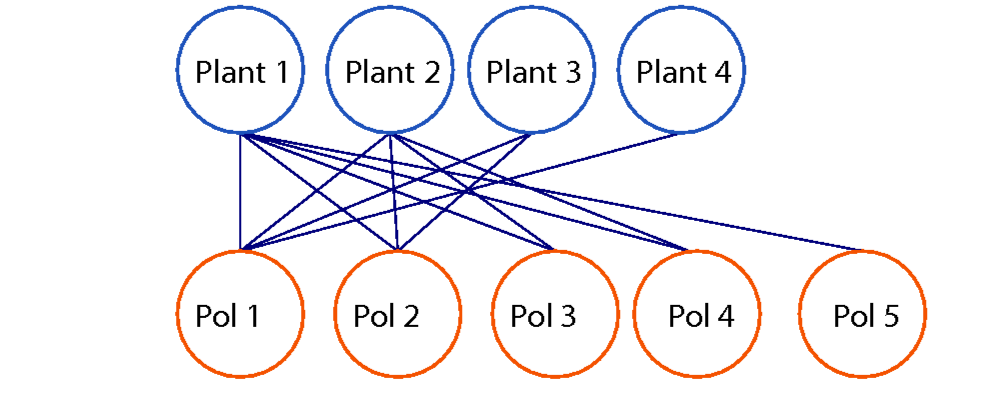
\includegraphics[scale=0.45]{DINAMICA_red_exper_2.png}
\caption {Comunidad mutualista con cinco especies de plantas y cuatro de polinizadores.}
\label{fig:red_exper_stab1}
\end{figure}

La figura \ref{fig:red_exper_stab1} muestra una pequeña comunidad mutualista ficticia, que hemos construido para los experimentos numéricos. Este ejemplo sencillo muestra la dinámica característica de las redes reales.

\begin{figure}[ht!]
\centering
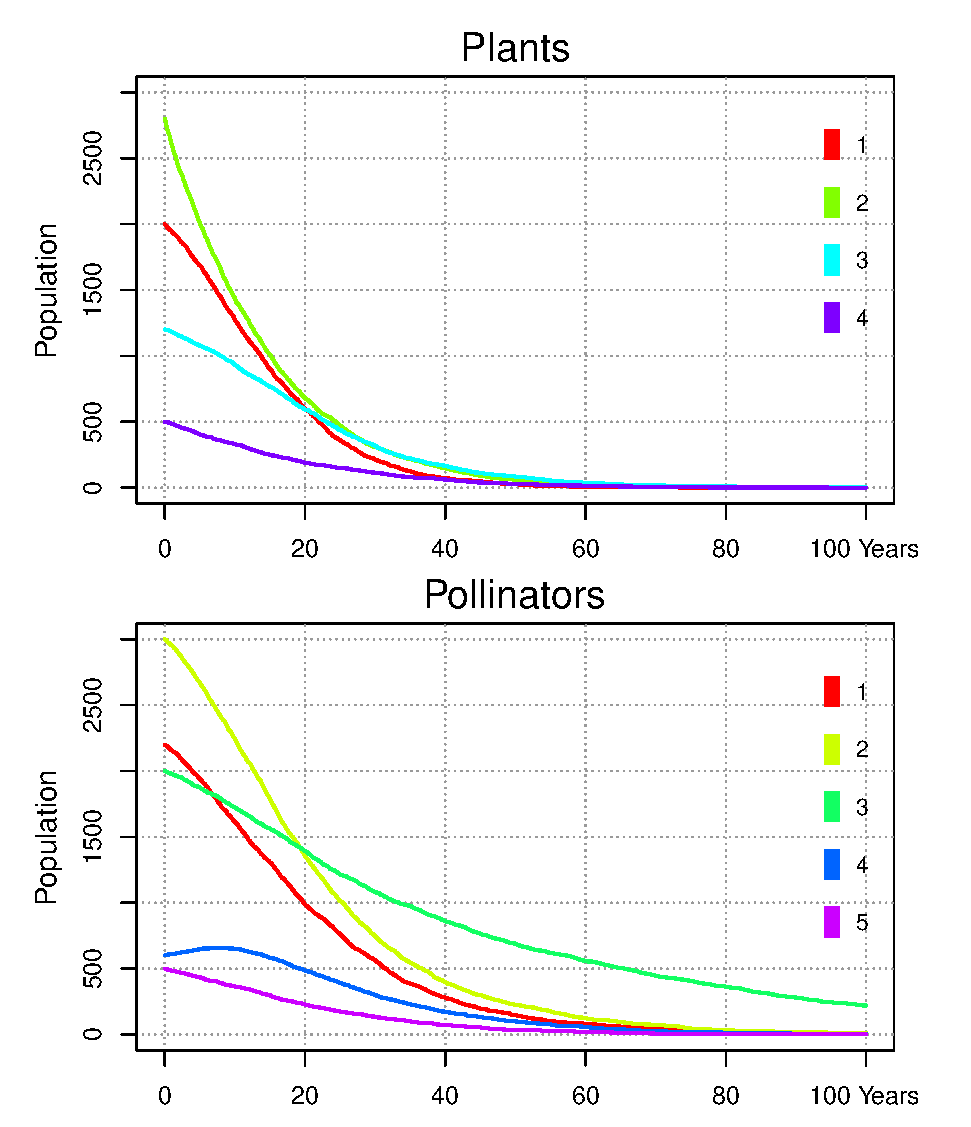
\includegraphics[width=8cm]{DINAMICA_Fig5_extinction.eps}
\caption {Dinámica de poblaciones para $4+5$ especies que termina en la extinción completa.}
\label{fig:exper_stab1}
\end{figure}

En el primer experimento (figura \ref{fig:red_exper_stab1}) el sistema empieza con todas las tasas efectivas negativas, excepto la del polinizador número $4$. Asumimos que el mutualismo es obligado. En estas circunstancias es sencillo encontrar los valores mínimos de población que garantizarían la supervivencia resolviendo $r_{\rm{eff}.i} = 0$ en las ecuaciones \ref{modelors}.

Las tasas efectivas solo pueden ser positivas por el beneficio mutualista, pero en esta simulación las poblaciones iniciales no son suficientes para para conseguirlo, con la excepción del mencionado polinizador número $4$. Las especies de planta $1$ y $2$ empiezan con poblaciones por encima de sus capacidades de carga.
Este experimento muestra el \textit{atractor de extinción} que conduce a la destrucción total de la comunidad.

\begin{figure}[ht!]
\centering
\includegraphics[scale = 0.66]{DINAMICA_Fig6_carrying_cap.eps}
\caption {Evolución temporal de las poblaciones y de las tasas de crecimiento efectivas del mismo sistema de $4+5$ species (figura \ref{fig:red_exper_stab1}). La comunidad termina con todas las especies en sus capacidades de carga respectivas.}
\label{fig:exper_carrying_cap}
\end{figure}

\begin{figure}[h!]
\centering
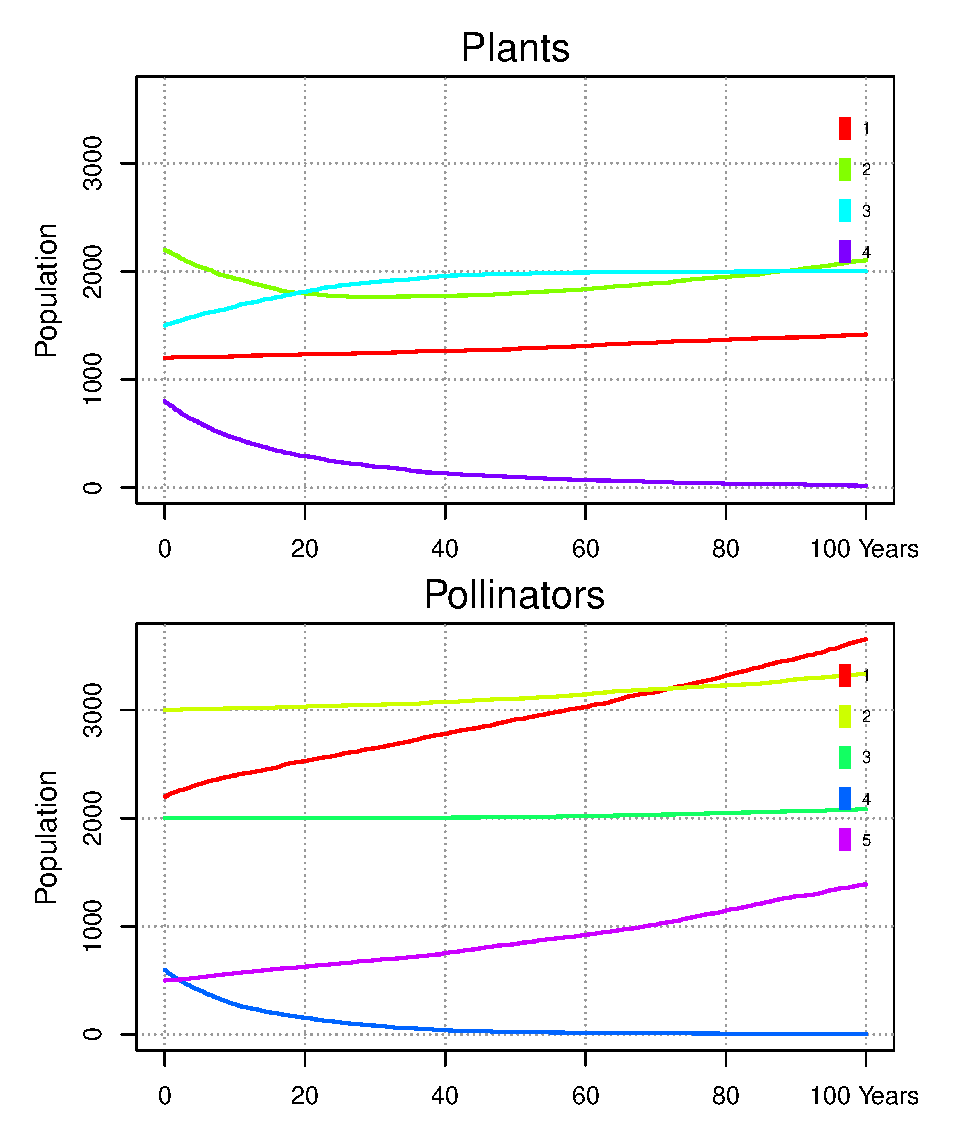
\includegraphics[scale = 0.66 ]{DINAMICA_Fig7_partial_extinct.eps}
\caption {Resultados del tercer experimento. El polinizador $4$ y la planta $4$ se extinguen.}
\label{fig:exper_stab2}
\end{figure}

La figura \ref{fig:exper_carrying_cap} muestra un segundo experimento, con la misma red, pero con diferentes parámetros (Anexo \ref{DINAMICA_ANEXO_KConst}). En esta simulación, todas las poblaciones de plantas iniciales están por debajo de sus capacidades de carga, pero con tasas de crecimiento efectivas positivas, por lo que terminan en máximos. La población del polinizador $5$ está inicialmente por encima de su capacidad de carga, por eso la tasa efectiva es ligeramente negativa y converge hacia la capacidad de carga al final de la simulación. Por el contrario, la especie de polinizador $4$ tiene muy pocos individuos al principio pero la abundancia de mutualistas genera una tasa eficaz positiva y una curva tipo de crecimiento logístico. Al final de la simulación todas las tasas efectivas convergen a cero, es el atractor que aparece en el máximo de poblaciones.

En la tercera simulación exploramos las extinciones parciales (figura \ref{fig:exper_stab2}). De nuevo, todas las tasas vegetativas son negativas, pero los pesos de los enlaces se han modificado ligeramente respecto al experimento anterior.

En esta simulación todas las poblaciones empiezan por debajo de sus capacidades de carga. Todas evolucionan hacia sus máximos excepto el polinizador $4$ y la planta $4$ que se extinguen. La especie de planta $2$ empieza con una tasa eficaz negativa pero el crecimiento de sus mutualistas da la vuelta a esta situación y termina sobreviviendo. Con estos tres casos se puede comprobar la riqueza dinámica de este modelo simple.

\subsection{Simulaciones con saturación del beneficio}
\label{results_alfa}

En este apartado presentamos los resultados de las simulaciones que hemos llevado a cabo con el modelo de saturación del beneficio mutualista (ecuaciones \ref{eq:DINAMICA_modeloralphaconmut}). Para el primer experimento hemos utilizado la misma red ficticia que en el apartado anterior (figura \ref{fig:red_exper_stab1})

\begin{figure}[b!]
\centering
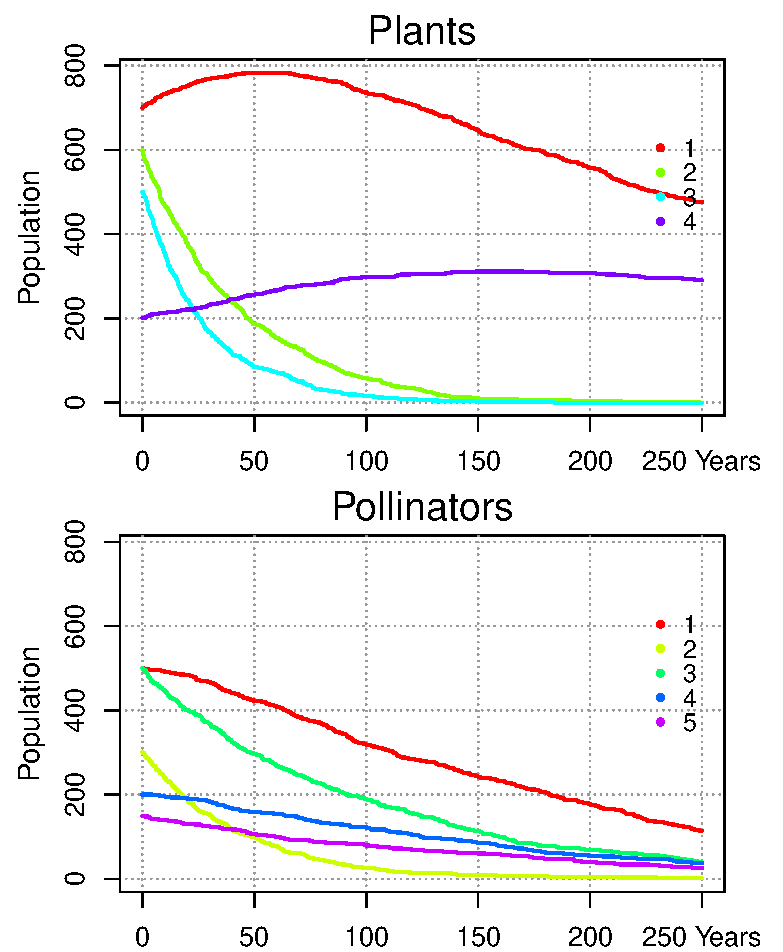
\includegraphics[scale=0.66]{DINAMICA_SATU_experimento_1.pdf}
\caption {Resultados del primer experimento. La parametrización puede verse en el Anexo \ref{DINAMICA_ANEXO_saturacion}, tabla \ref{tab:SAT_experiment1}.}
\label{fig:DINAMICA_SAT_exper_stab1}
\end{figure}

En todos los experimentos las tasas vegetativas son negativas, el mutualismo es obligado para todas las especies.

El primer experimento con saturación (figura \ref{fig:DINAMICA_SAT_exper_stab1}) es similar al realizado para el modelo con capacidades de carga constantes. En este caso, hay especies que empiezan la simulación con tasas efectivas negativas y otras positivas, pero el sistema está al principio por debajo de la divisoria multidimensional y se extingue porque la trayectoria termina en el atractor de destrucción.

\begin{figure}[h!]
\centering
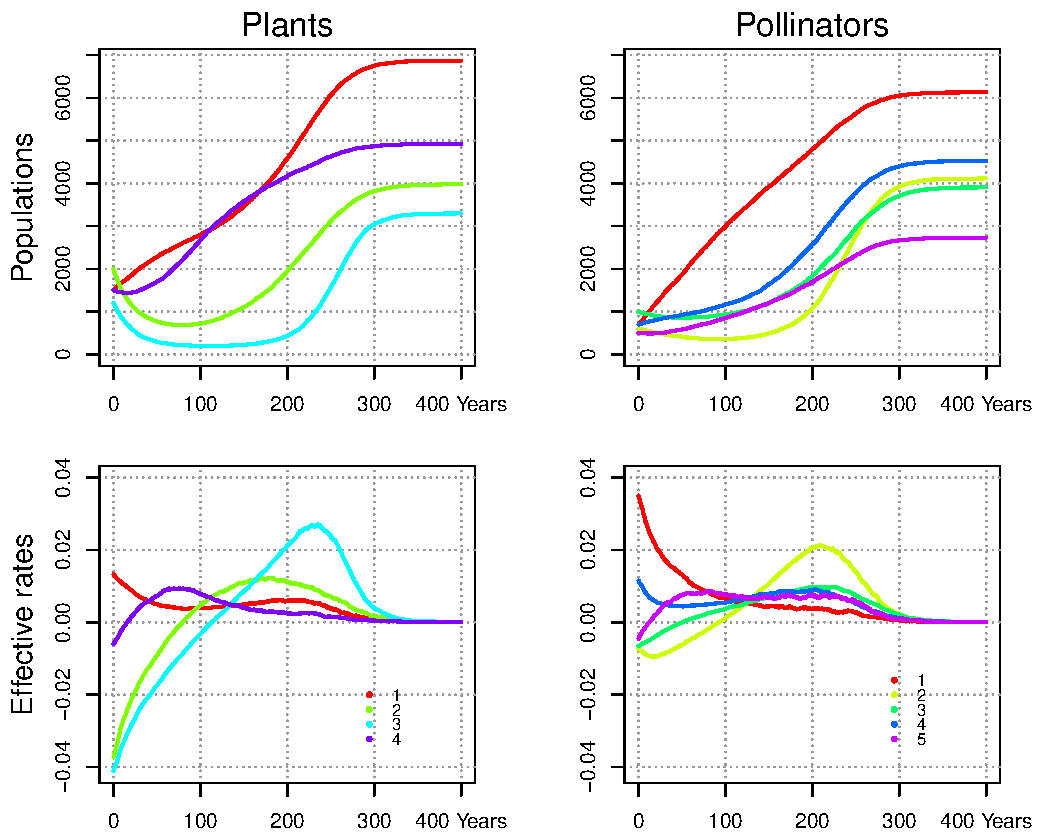
\includegraphics[scale=0.8]{DINAMICA_SATU_experimento_2.pdf}
\caption {Resultados del segundo experimento. La configuración puede consultarse en el Anexo  \ref{DINAMICA_ANEXO_saturacion}, tabla \ref{tab:SAT_experiment2}.}
\label{fig:DINAMICA_SAT_exper_stab2}
\end{figure}

La segunda simulación (figura \ref{fig:DINAMICA_SAT_exper_stab2}) muestra como el sistema evoluciona hasta máximos de todas las especies. En este caso resulta de gran interés ver como varían las tasas de crecimiento eficaces y la complejidad que pueden llegar a adquirir por las múltiples interacciones. Al final todas terminan anulándose porque el sistema ha alcanzado el punto de equilibrio máximo. 

Los análisis de estabilidad de este capítulo asumían que las condiciones no se alteran durante el estudio. En realidad, las tasas varían como consecuencia de diferentes perturbaciones medioambientales. A continuación, vamos a ver la resistencia del sistema ante perturbaciones externas, simulando fuertes incrementos en las tasas de mortalidad $r_{d_i}$ como las que producen las sequías o las enfermedades. La literatura afirma que el \emph{anidamiento} proporciona resistencia a las comunidades \citep{bascompte2003nested}. Los dos últimos experimentos muestran como influye esta magnitud.

\begin{figure}[h!]
\centering
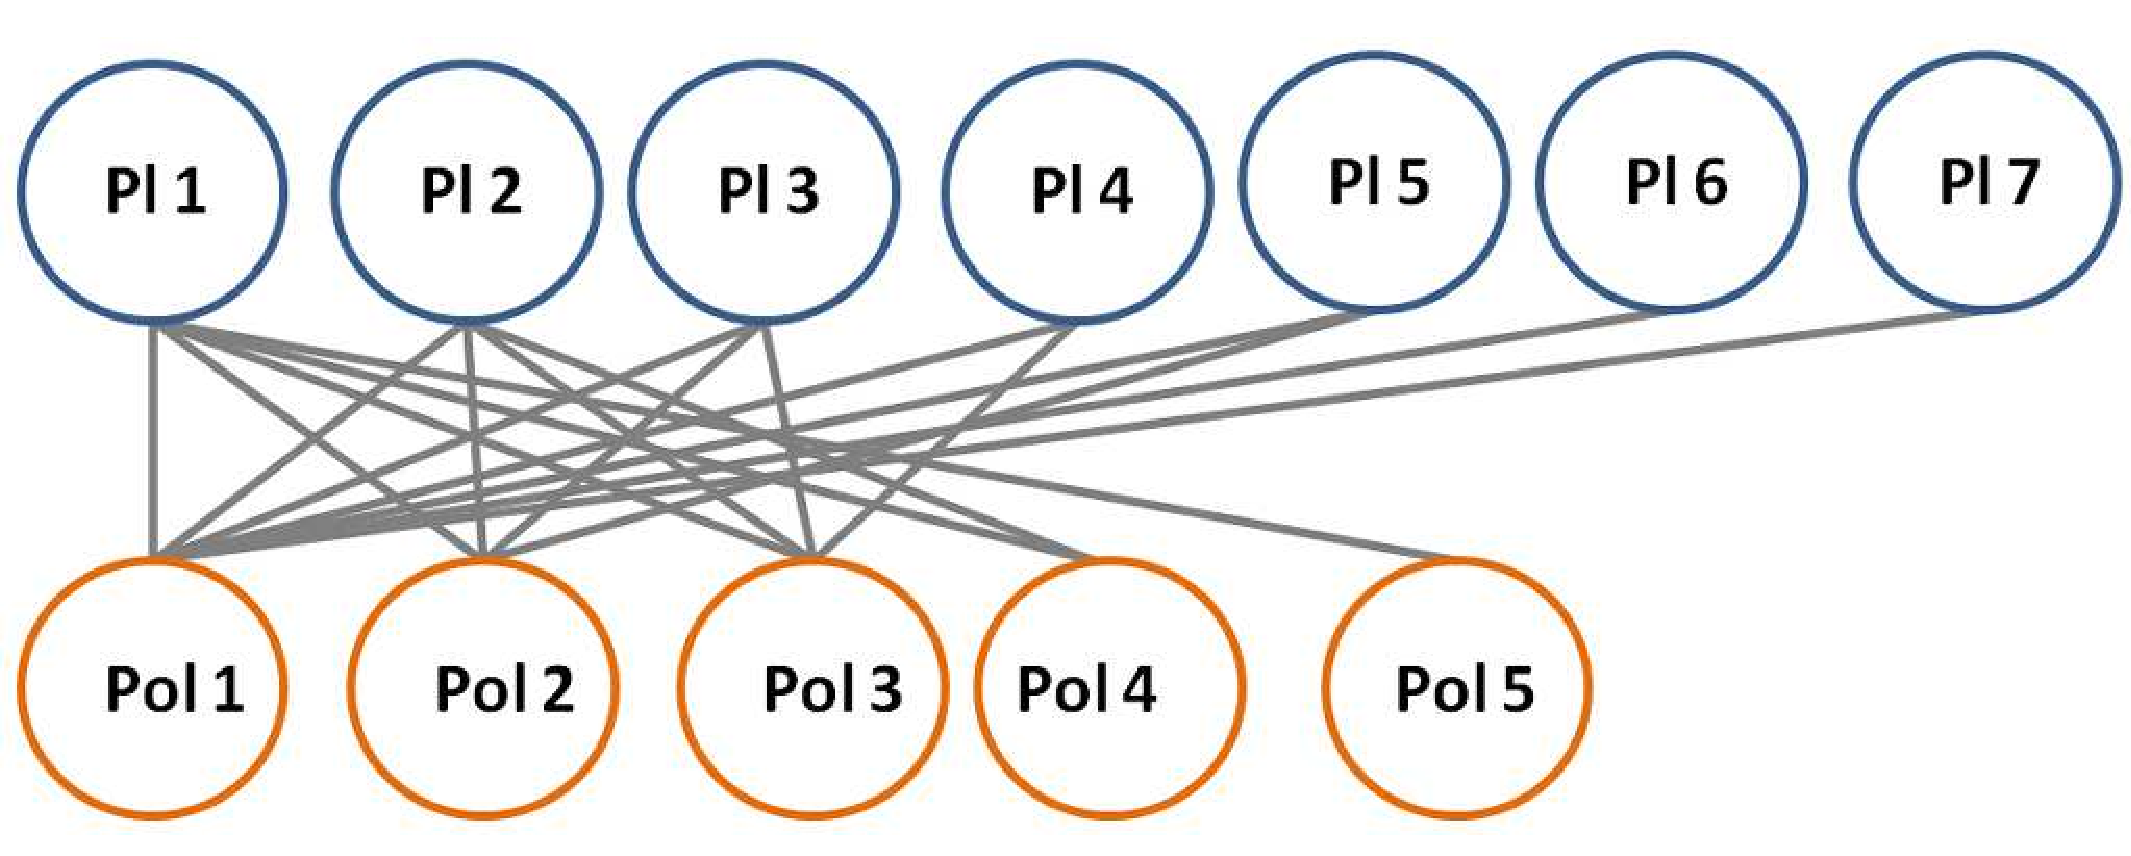
\includegraphics[scale=0.28]{DINAMICA_SAT_red_exper_resilience_strong.pdf}
\caption {Red con anidamiento fuerte ($NODF = 93.55$). Tabla \ref{tab:SAT_exper_resilience_strong}.}
\label{fig:DINAMICA_SAT_red_exper_resilience_strong}
\end{figure}

En el penúltimo usamos otra red ficticia, con siete especies de plantas y cinco de polinizadores (figura \ref{fig:DINAMICA_SAT_red_exper_resilience_strong}). Puede identificarse de manera visual el núcleo central de especies generalistas y las especies especialistas conectadas a generalistas de la clase contraria. Se han elegido las poblaciones iniciales para que el sistema esté en la cuenca de supervivencia.

\begin{figure}[h!]
\centering
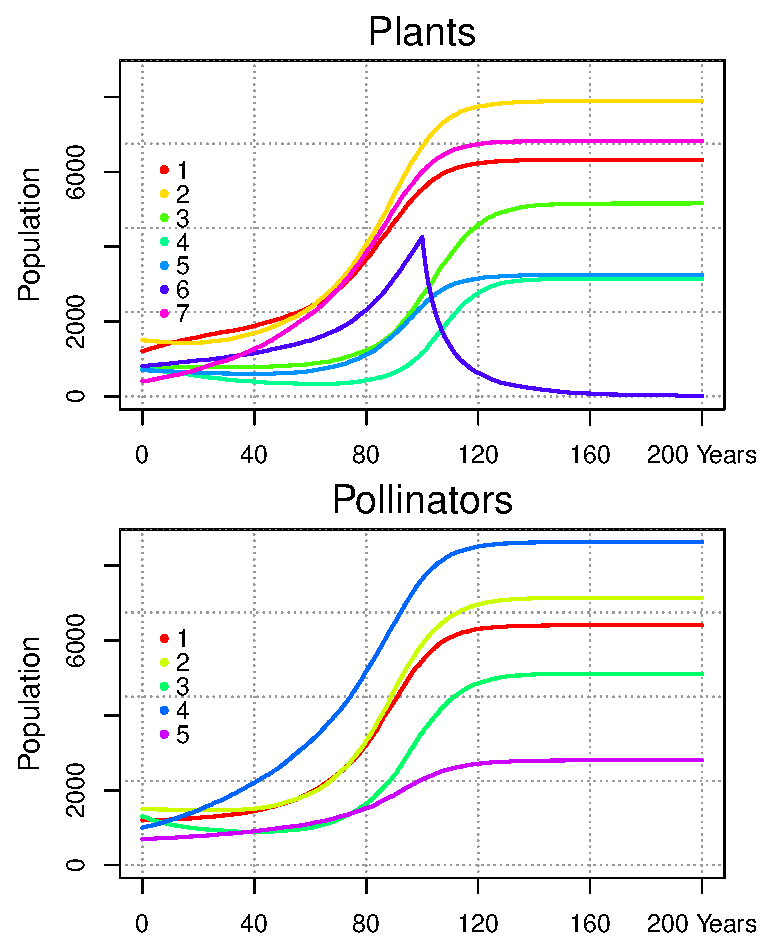
\includegraphics[scale=0.75]{DINAMICA_SATU_nested.pdf}
\caption {Experimento con la red con anidamiento fuerte. Una perturbación externa ataca la especie de planta número $6$. Tabla \ref{tab:SAT_exper_resilience_strong}.}
\label{fig:DINAMICA_SAT_exper_resilience_strong}
\end{figure}

El sistema crecería hasta alcanzar máximos en ausencia de perturbaciones externas, pero sobre la especie $6$ de plantas provocamos un aumento abrupto de mortalidad de un $20\%$ anual que la conduce a la extinción. Esta especie estaba conectada solo al polinizador $1$, el más generalista de su clase. El efecto de la extinción es despreciable sobre este polinizador porque el resto de especies benefactoras lo suplen. 

\begin{figure}[h!]
\centering
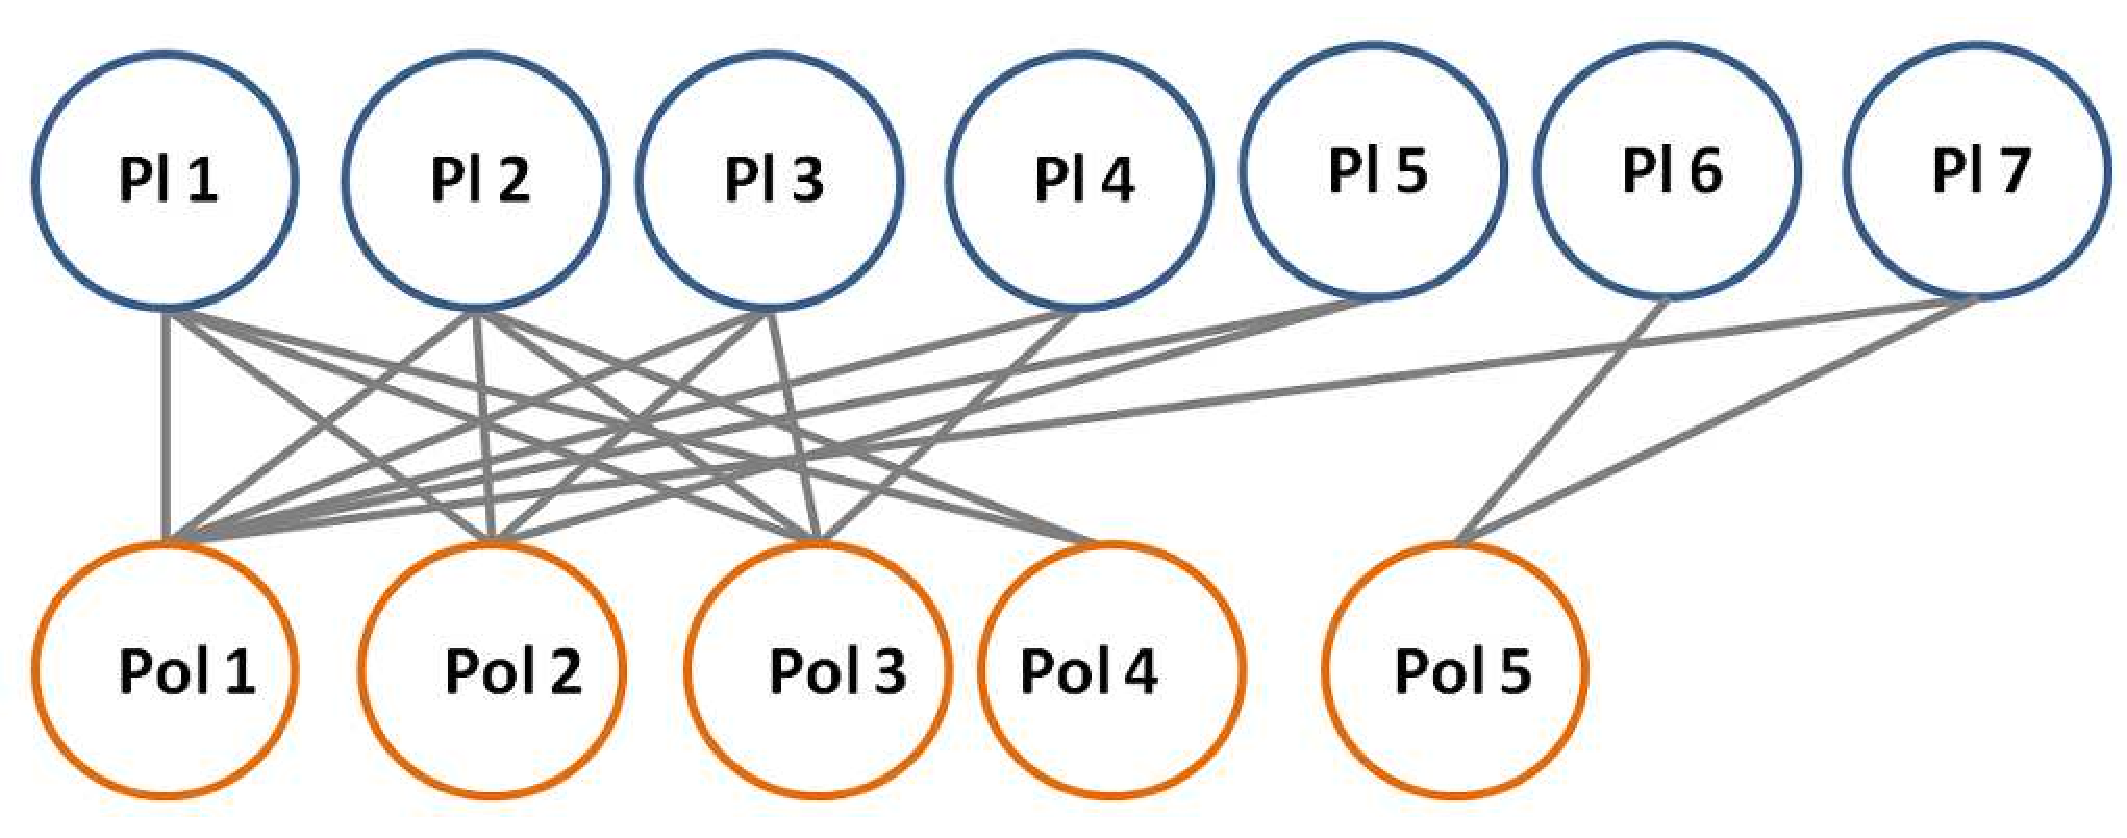
\includegraphics[scale=0.28]{DINAMICA_SAT_red_exper_resilience_weak.pdf}
\caption {Red débilmente anidada. Tabla \ref{tab:SAT_exper_resilience_weak}.}
\label{fig:DINAMICA_SAT_red_exper_resilience_weak}
\end{figure}

El último experimento usa una red ligeramente modificada (figura  \ref{fig:DINAMICA_SAT_red_exper_resilience_weak}). La especie de plantas $6$ se conecta al polinizador $5$, un especialista. También se elimina el enlace que conecta la planta $1$ con el polinizador $5$ y se reemplaza por uno nuevo entre la planta $7$ y el polinizador $1$.  

\begin{figure}[ht!]
\centering
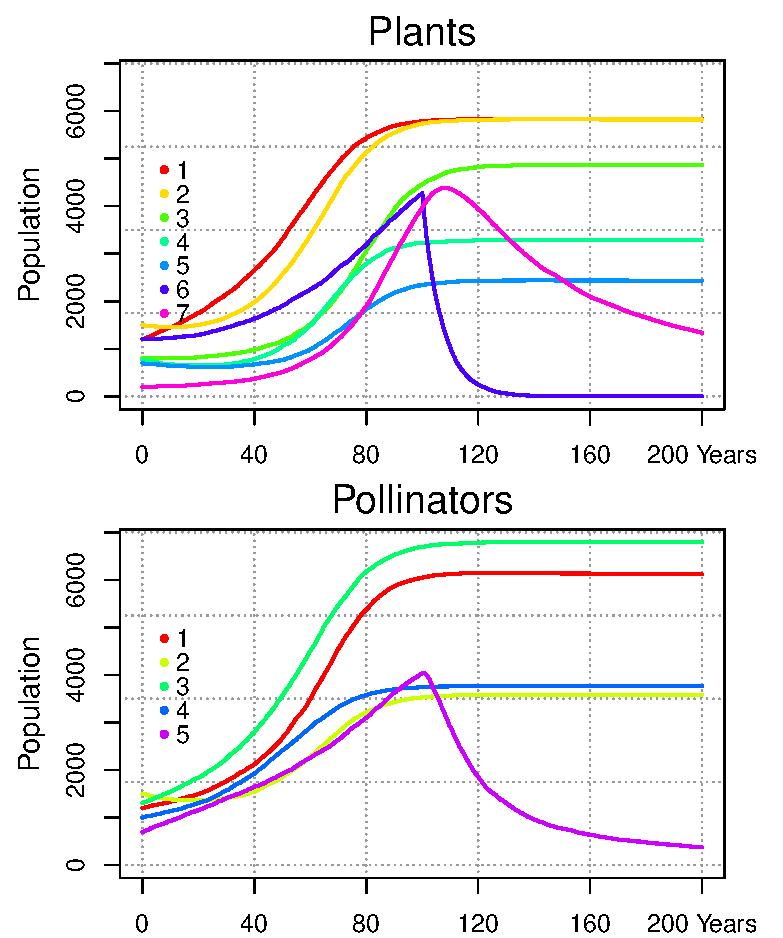
\includegraphics[scale=0.85]{DINAMICA_SATU_weak.pdf}
\caption {Experimento con una red menos anidada ($NODF = 26.39$). Una perturbación externa ataca la planta $6$. Tabla \ref{tab:SAT_exper_resilience_weak}.}
\label{fig:DINAMICA_SAT_exper_resilience_weak}
\end{figure}

Las posibilidades de supervivencia de una nueva especie que llegue a la comunidad son mayores si se conecta con una generalista. Esta propiedad se debe no solo al hecho de que las generalistas son menos vulnerables por la gran cantidad de especies de las que reciben beneficio. Enlazarse con una especialista expone a la destrucción por arrastre.

Cuando la planta $6$ es atacada y se extingue el efecto es mucho peor para la red. El polinizador $5$ pierde a su única especie benefactora, de manera que su tasa efectiva se vuelve negativa y finalmente desaparecerá. La planta $7$, conectada con el polinizador $5$ también se ve condenada a la extinción porque su enlace con el polinizador $1$ no compensa la pérdida. En resumen, una perturbación externa sobre la especie de planta $6$ arrastra a la extinción a la planta $7$ por culpa del enlace que comparten con el polinizador $5$. Si ambas plantas compartieran enlaces con el núcleo generalista esta destrucción en cascada resultaría mucho más improbable.

%\section{Conclusiones}
%
%En este capítulo, se han presentado dos modelos de dinámica mutualista derivados de la ecuación logística. Ambos solucionan los problemas de estabilidad del modelo de May y la paradoja de Levins, derivada de la fórmula de Pearl, y permiten un tratamiento analítico más simple que los llamados de \textit{tipo II}.
%
%El primero funciona con capacidad de carga constante, con independencia de la abundancia de individuos de las especies mutualistas. Es una modificación muy simple, que permite describir la dinámica habitual del mutualismo, sus puntos fijos y el \textit{saddle} que marca la supervivencia de la comunidad. Se puede resolver de forma analítica y extender del caso simple de dos especies al más general. Las simulaciones numéricas han permitido reproducir lo que preveía el análisis.
%
%El segundo modelo es más refinado. En lugar de forzar la estabilidad mediante una capacidad de carga constante, el crecimiento se limita automáticamente con un término adicional lineal en el coeficiente de fricción intra especie. Este parámetro aparecía de manera natural en la formulación original de Verhulst, por lo que la extensión a partir de ella es mucho más evidente que con la fórmula de Pearl.
%
%El análisis de estabilidad es más simple para este modelo que para el primero que hemos propuesto y que para los modelos habituales de la literatura. Además, se ha explicado como se puede encontrar la divisoria que separa las cuencas de extinción y supervivencia, que es una ley de potencia para el caso de dos especies.
%
%La simulación estocástica a la hora de integrar las ecuaciones, permite introducir de manera muy simple perturbaciones externas que suceden en de manera habitual en la naturaleza. Los experimentos numéricos con este modelo y unas redes muy simples han mostrado la gran riqueza y complejidad de la dinámica del mutualismo.

\clearpage
\section{Anexo: Análisis en detalle de la estabilidad del modelo con saturación}
\label{DINAMICA_ANEXO_estabilidad}

Para simplificar, prescindimos de los superíndices que representan las clases $animal$ y $planta$. 
El sistema de ecuaciones \ref{eq:DINAMICA_dos_especies} se desarrolla en serie de Taylor en la vecindad del punto singular ($N^{*}_{1}, N^{*}_{2}$) como  $N_{1}= N^{*}_1+\tilde{N}_{1}$ y $N_{2}= N^{*}_2+\tilde{N}_{2}$ \cite{murray1993mathematical}:

\begin{equation}
\begin{array}{lcr}
\displaystyle \frac{d\tilde{N}_{1}}{dt} = r_{1}+ b_{12}(N^{*}_2+\tilde{N}_{2})-(\alpha_{1}+ c_{1} b_{12} (N^{*}_2+\tilde{N}_{2}))( N^{*}_1+\tilde{N}_{1})\nonumber\\
\\
\displaystyle \frac{d\tilde{N}_{2}}{dt} = r_{2}+ b_{21}( N^{*}_1+\tilde{N}_{1})-(\alpha_{2}+ c_{2} b_{21}(N^{*}_1+\tilde{N}_{1}))(N^{*}_2+\tilde{N}_{2}) 
\stepcounter{equation}\tag{\theequation}\label{eq:effrateTaylor}
\end{array}
\end{equation}

\noindent y quedándonos solo con los términos de primer orden:

\begin{equation}
\begin{array}{lcr}
\displaystyle \frac{d\tilde{N}_{1}}{dt}= \tilde{N}_{2}( b_{12} - c_{1} b_{12}\, N^{*}_1)-\tilde{N}_{1}(\alpha_{1}+ c_{1} b_{12} \, N^{*}_2) \equiv f_{1}(\tilde{N}_{1},\tilde{N}_{2}) \nonumber\\
\\
\displaystyle \frac{d\tilde{N}_{2}}{dt} = \tilde{N}_{1}( b_{21} - c_{2} b_{21}\, N^{*}_2)-\tilde{N}_{2}(\alpha_{2}+ c_{2} b_{21} \, N^{*}_1) \equiv f_{2}(\tilde{N}_{1},\tilde{N}_{2})
\stepcounter{equation}\tag{\theequation}\label{eq:effrateTaylor2}
\end{array}
\end{equation}

\noindent Los términos del jacobiano son:

\begin{equation}
\begin{array}{l}
J_{11}= \frac{\partial f_{1}}{\partial \tilde{N}_{1}} =- N^{*}_{1}\left(\alpha_{1}+ c_{1} b_{12} \, N^{*}_2\right)  \\
\\
J_{12}= \frac{\partial f_{1}}{\partial \tilde{N}_{2}} = N^{*}_{1}b_{12}\left(1 - c_{1}\, N^{*}_1\right) \\
\\
J_{21}= \frac{\partial f_{2}}{\partial \tilde{N}_{1}} = N^{*}_{2}b_{21} \left(1 - c_{2}\, N^{*}_2\right) \\
\\
J_{22}= \frac{\partial f_{2}}{\partial \tilde{N}_{2}} = - N^{*}_{2}\left(\alpha_{2}+ c_{2} b_{21}\,N^{*}_{1}\right)
\end{array}
\stepcounter{equation}\tag{\theequation}\label{eq:J11}
\end{equation}

\noindent que puede reescribirse en términos de los coeficientes positivos $J_{ij}$ como:

\begin{equation*}
J = \left(
\begin{array}{rr}
-J_{11} & J_{12} \\ J_{21} & -J_{22}
\end{array}
\right)
\end{equation*}

\noindent Los autovalores $\lambda_{1,2}$ se obtienen de
\begin{equation}
\lvert J - \lambda I \rvert =0
\stepcounter{equation}\tag{\theequation}\label{eq:lambda0App}
\end{equation}

\noindent cuyas soluciones son
\begin{equation}
\begin{array}{lcl}
\lambda _{1,2}=\frac{1}{2}\left(tr(J)\pm \sqrt{tr^{2}(J)-4\,\mathrm{Det}(J)}\right)\\ =
\frac{1}{2}\left(-\left(J_{11}+J_{22}\right)\pm \sqrt{\left(J_{11}+J_{22}\right)^{2}-4\,\mathrm{Det}(J)}\right)\\  =
\frac{1}{2}\left(-\left(J_{11}+J_{22}\right)\pm \sqrt{\left(J_{11}-J_{22}\right)^{2} +4 \,\left( J_{12}J_{21} \right) }\right)
\end{array}
\stepcounter{equation}\tag{\theequation}\label{eq:lambda12}
\end{equation}

\noindent La última expresión indica que los dos autovalores son reales. Además, satisfacen la siguiente condición:

\begin{equation}
\prod_{k}\lambda_{k}=\mathrm{Det}(J)
\end{equation}

\noindent por tanto el punto singular será un \textit{saddle point} cuando se cumpla que  $\mathrm{Det}(J)<0$. Expandiendo el determinante del jacobiano obtenemos la condición de existencia del \textit{saddle point}:

\begin{equation}
1-c_{1}N^{*}_{1}-c_{2}N^{*}_{2} >0
\end{equation}

Las extinciones parciales son también puntos singulares, y corresponden a $N^{*}_{1,2} = 0$. Para simplificar, escribimos solo las ecuaciones del punto singular  ($N^{*}_{1}=r_{1}/\alpha_{1},N^{*}_{2}=0$). Expandiendo en serie de Taylor en torno a él, el sistema de ecuaciones se convierte en:

\begin{equation}
\begin{array}{ll}
\displaystyle \frac{d\tilde{N}_{1}}{dt} = & r_{1} N^{*}_{1}-\alpha_{1}N^{*2}_{1}+r_{1}\tilde{N}_{1}+ b_{12}\tilde{N}_{2}N^{*}_1-2\alpha_{1}N^{*}_1\tilde{N}_{1} + \\
\, & - c_{1} b_{12}\tilde{N}_{2}N^{*2}_1\nonumber\\
\displaystyle \frac{d\tilde{N}_{2}}{dt} = & r_{2}\tilde{N_{2}}+ b_{21} N^{*}_1\tilde{N_{2}} 
\end{array}
\label{eq:effrateTaylorN2=0}
\end{equation}

\noindent El jacobiano es ahora:

\begin{equation*}
J = \left(
\begin{array}{rr}
-r_{1} & b_{12}N^{*}_{1}\left(1-c_{1}N^{*}_{1}\right) \\
0 & r_{2}+b_{21}N^{*}_{1}
\end{array}
\right)
\end{equation*}

Los autovalores son los términos de la diagonal. Este punto será estable si se cumple que $r_{1}>0$ y que $r_{2}<-b_{21}r_{1}/\alpha_{1}$. La solución simétrica es ($N^{*}_{1}=0,N^{*}_{2}=r_{2}/\alpha_{2}$) y será estable si  $r_{2}>0$ y $r_{1}<-b_{12}r_{2}/\alpha_{2}$. La generalización para $n_{a} + n_{p}$ especies es:
 
\begin{align}
\frac{dN_{i}}{dt} = \left( r_{i}+ \sum_{j=1}^{n_{a}} b_{ij}N_{j}\right)N_{i} - \left(\alpha_{i}+ c_{i} \sum_{j=1}^{n_{a}} b_{ij}N_{j} \right) N^{2}_{i} \nonumber\\ 
\frac{dN_{j}}{dt} = \left( r_{j}+ \sum_{i=1}^{n_{p}} b_{ji}N_{i}\right)N_{j} - \left(\alpha_{j}+ c_{j} \sum_{i=1}^{n_{p}} b_{ji} N_{i} \right) N^{2}_{j} 
\stepcounter{equation}\tag{\theequation}\label{eq:N_especies}
\end{align}

\noindent donde el subíndice $i$ se extiende para todas las especies de plantas y el $j$ para todas las de animales.

Los puntos fijos de este sistema son la solución trivial de destrucción completa de la comunidad ($N_{i=1\cdots n_{p}}=0, N_{j=1\cdots n_{a}}=0$), y las soluciones para las que las tasas de crecimiento efectivas se anulan: 

\begin{equation}
\begin{array}{lcr}
\displaystyle r^{*}_{eff,i} =\left(r_{i}+ \sum_{j=1}^{n_{a}} b_{ij}N^{*}_{j}\right)- \left(\alpha_{i}+c_{i}\sum_{j=1}^{n_{a}} b_{ij}N^{*}_j\right)N^{*}_{i}
=0 \nonumber\\
\displaystyle r^{*}_{eff,j} = \left(r_{j}+ \sum_{i=1}^{n_{p}} b_{ji}N^{*}_{i}\right)- \left(\alpha_{j}+c_{j}\sum_{i=1}^{n_{p}} b_{ji}N^{*}_i\right)N^{*}_{j} 
=0 
\stepcounter{equation}\tag{\theequation}\label{eq:effrateN}
\end{array}
\end{equation}

\noindent que pueden reescribirse como un conjunto de ecuaciones implícitas.

\begin{eqnarray}
\begin{array}{lcc}
  N^{*}_{i}=\frac{r_{i}+\sum_{j=1}^{n_{a}}b_{ij}N^{*}_{j}}{\alpha_{i}+c_{i}\sum_{i=1}^{n_{p}}b_{ij}N^{*}_{j}} = 
  \frac{r_{i}+r_{i}^{Mut}}{\alpha_{i}+c_{i}r_{i}^{Mut}} = 
  \frac{r_{i}^{*+}}{r_{i}^{*-}}  \nonumber\\
  \\
  N^{*}_{j}=\frac{r_{j}+\sum_{i=1}^{n_{p}}b_{ji}N^{*}_{i}}{\alpha_{j}+c_{j}\sum_{i=1}^{n_{a}}b_{ij}N^{*}_{i}} =
  \frac{r_{j}+r_{j}^{Mut}}{\alpha_{j}+c_{j}r_{j}^{Mut}} =
  \frac{r_{j}^{*+}}{r_{j}^{*-}}
  \end{array}
\end{eqnarray} 
 
\noindent donde las tasas $r^{*+}$ y $r^{*-}$ representan el efecto positivo sobre el crecimiento y el negativo, respectivamente. El sistema \ref{eq:N_especies} puede también desarrollarse en torno al punto singular:

\begin{equation}
\begin{array}{lcl}
\textstyle \frac{dN_{i}}{dt}=r_{i}+\sum\limits_{j=1}^{n_{a}}b_{ij}(N^{*}_{j}+\tilde{N}_{j})- (\alpha_{i}+c_{i}\sum\limits_{j=1}^{n_{a}}b_{ij}(N^{*}_j+\tilde{N}_{j}))(N^{*}_i+\tilde{N}_{i}) \nonumber\\
\textstyle \frac{dN_{j}}{dt}=r_{j}+\sum\limits_{i=1}^{n_{p}}b_{ji}(N^{*}_{i}+\tilde{N}_{i})-(\alpha_{j}+c_{j}\sum\limits_{i=1}^{n_{p}}b_{ji}(N^{*}_i+\tilde{N}_{i}))(N^{*}_j+\tilde{N}_{j}) 
\stepcounter{equation}\tag{\theequation}\label{eq:effrateTaylorN}
\end{array}
\end{equation}

\noindent donde el subíndice $i$ corresponde a las plantas y el $j$ a los animales. El conjunto de $n_{a} + n_{p}$ ecuaciones se reescribe en términos lineales como:

\begin{align}
\begin{array}{lcl}
\displaystyle \frac{dN_{i}}{dt} = \sum_{j=1}^{n_{a}} \tilde{N}_{j} \left(  b_{ij} - c_{i} b_{ij}\, N^{*}_i\right) - \tilde{N}_{i}(\alpha_{i}+ c_{i} \sum_{j=1}^{n_{a}} b_{ij} \, N^{*}_{j})\nonumber\\
\displaystyle \frac{dN_{j}}{dt} = \sum_{i=1}^{n_{p}} \tilde{N}_{i} \left( b_{ji} - c_{j} b_{ji}\, N^{*}_j\right) - \tilde{N}_{j}(\alpha_{j}+ c_{j} \sum_{i=1}^{n_{p}} b_{ji} \, N^{*}_{i})\stepcounter{equation}\tag{\theequation}\label{eq:effrateTaylor2N}
\end{array}
\end{align}

Los coeficientes de $\tilde{N}_{i,j}$ son los términos del jacobiano. Los valores absolutos de los elementos de la diagonal, para cualquier especie $i$ de plantas, $j$ de animales son:

\begin{align}
\displaystyle & J_{ii}=N^{*}_{i}\left(\alpha_{i} + c_{i} \sum_{j=1}^{n_{a}} b_{ij} N^{*}_{j}\right) \nonumber\\
\displaystyle & J_{jj}=N^{*}_{j}\left(\alpha_{j} + c_{j} \sum_{i=1}^{n_{p}} b_{ji} N^{*}_{i}\right)
\label{eq:Jii2}
\end{align}

\noindent y los términos fuera de la diagonal:

\begin{align}
\displaystyle & J_{ij}=N^{*}_{i}b_{ij}\left( 1-c_{i}N^{*}_{i}\right)\nonumber\\
\displaystyle & J_{ji}=N^{*}_{j}b_{ji}\left( 1-c_{j}N^{*}_{j}\right)
\label{eq:Jij}
\end{align}

\noindent Como resultado el jacobiano queda así:

\begin{equation*}
J=\left(
   \begin{array}{ccccc}
      \ddots  & \cdots & \cdots & \cdots & \cdots \\
      \cdots  & -J_{ii} & \cdots & J_{ij} & \cdots \\
      \vdots  & \vdots & \ddots  & \vdots & \vdots  \\
      \cdots  & J_{ji} & \cdots & -J_{jj} & \cdots \\
      \cdots  & \cdots & \cdots & \cdots  & \ddots
   \end{array}
\right)
\end{equation*}

\noindent con todos los términos de la diagonal negativos y el resto positivos. La suma de los autovalores satisface la sigiente igualdad:

\begin{equation}
  \sum_{k}^{n_{a}+n_{p}} \lambda_{k}= -\left(\sum_{k}^{n_{a}+n_{p}} J_{kk}\right)
  \stepcounter{equation}\tag{\theequation}\label{eq:sum_lambdas}
\end{equation}

Esto significa que no todos los autovalores son positivos y que por tanto el punto singular no es asintóticamente inestable. Por otra parte, los autovalores no pueden ser complejos porque todos los coeficientes fuera de la diagonal son positivos o nulos; los puntos fijos deben ser estables o  \textit{saddle point}.

\clearpage
\section{Anexo: Datos de las simulaciones del modelo con \textit{K} constantes}
\label{DINAMICA_ANEXO_KConst}

\begin{table}[h!]
\centering
\footnotesize
\begin{tabular}{lrrrr}
\hline
 & Planta 1 & Planta 2 & Planta 3 & Planta 4  \\
\hline
\\
$b_{pol1j}\left(10^{-6}\right)$ & 1 & 12 & 12 & 16 \\
$b_{pol2j}\left(10^{-6}\right)$ & 20 & 4 & 11 & 0 \\
$b_{pol3j}\left(10^{-6}\right)$ & 20 & 10 & 0 & 0 \\
$b_{pol4j}\left(10^{-6}\right)$ & 10 & $0.1$ & 0 & 0 \\
$b_{pol5j}\left(10^{-6}\right)$ & 10 & 0 & 0 & 0 \\
$N_{init\,j}$ & 2000 & 2800 & 1200 & 500 \\
$K_{j}$ & 1500 & 2500 & 2000 & 1000 \\
$r_{birth\, j}$ & 0.004 & 0.01 & 0.01 & 0.005 \\
$r_{death\, j}$ & 0.13 & 0.10 & 0.08 & 0.065 \\
\hline
\\
\end{tabular}

\begin{tabular}{lrrrrr}
\hline
 &Pol 1&Pol 2&Pol 3&Pol 4&Pol 5\\
\hline
\\
$b_{pl1m}\left(10^{-6}\right)$ & 4 & 13 & 5 & 30 & 20\\
$b_{pl2m}\left(10^{-6}\right)$ & 12 & 6 & 10 & $0.1$ & 0\\
$b_{pl3m}\left(10^{-6}\right)$ & 2 & 5 & 0 & 0 & 0\\
$b_{pl4m}\left(10^{-6}\right)$ & 10 & 0 & 0 & 0 & 0\\
$N_{init\,m}$ & 3000 & 3000 & 2000 & 600 & 500 \\
$K_{m}$& 5000 & 4000 & 3000 & 2000 & 2000\\
$r_{b\, m}$ & 0.08 & 0.02 & 0.05 & 0.08 & 0.02 \\
$r_{d\, m}$ & 0.14 & 0.078 & 0.07 & 0.14 & 0.08 \\
\hline
\end{tabular}
\normalsize
\caption{Coeficientes mutualistas y condiciones del primer experimento del modelo con capacidades de carga constantes (fig. \ref{fig:exper_stab1}), con la red de la figura \ref{fig:red_exper_stab1}. Arriba, la matriz polinizador-planta, abajo la planta-polinizador.}
\label{tab:experiment1}\vspace*{-10pt}
\end{table}

\begin{table}[h!]
\centering
\footnotesize
\begin{tabular}{lrrrr}
\hline
 & Planta 1 & Planta 2 & Planta 3 & Planta 4  \\
\hline
\\
$b_{pol1j}\left(10^{-6}\right)$ & 50 & 22 & 42 & 56 \\
$b_{pol2j}\left(10^{-6}\right)$ & 20 & 40 & 81 & 0 \\
$b_{pol3j}\left(10^{-6}\right)$ & 20 & 10 & 0 & 0 \\
$b_{pol4j}\left(10^{-6}\right)$ & 50 & $0.1$ & 0 & 0 \\
$b_{pol5j}\left(10^{-6}\right)$ & 10 & 0 & 0 & 0 \\
$N_{init\,j}$ & 1500 & 1200 & 1000 & 500 \\
$K_{j}$ & 2800 & 2500 & 2000 & 1000 \\

\hline
\\
\end{tabular}

\begin{tabular}{lrrrrr}
\hline
 &Pol 1&Pol 2&Pol 3&Pol 4&Pol 5\\
\hline
\\
$b_{pl1m}\left(10^{-6}\right)$ & 40 & 13 & 15 & 30 & 20\\
$b_{pl2m}\left(10^{-6}\right)$ & 12 & 6 & 1 & 1 & 0\\
$b_{pl3m}\left(10^{-6}\right)$ & 2 & 5 & $0.1$ & 0 & 0\\
$b_{pl4m}\left(10^{-6}\right)$ & 1 & 1 & 0 & 0 & 0\\
$N_{init\,m}$ & 2200 & 3000 & 2000 & 600 & 2200 \\
$K_{m}$& 5000 & 4000 & 3000 & 2000 & 2000\\
\hline
\end{tabular}
\normalsize
\caption{Configuración del experimento de la figura \ref{fig:exper_stab2} Las tasas de nacimiento y muerte son las mismas que en la tabla \ref{tab:experiment1} excepto $r_{d,pl3}=0.1$, $r_{d,pol2}=0.048$ y $r_{d,pol5}=0.04$}
\label{tab:experiment2}
\end{table}


\begin{table}[h!]
\centering
\footnotesize
\begin{tabular}{lrrrr}
\hline
 & Planta 1 & Planta 2 & Planta 3 & Planta 4  \\
\hline
\\
$b_{pol1j}\left(10^{-6}\right)$ & 10 & 22 & 42 & 6 \\
$b_{pol2j}\left(10^{-6}\right)$ & 20 & 4 & 11 & 0 \\
$b_{pol3j}\left(10^{-6}\right)$ & 20 & 10 & 0 & 0 \\
$b_{pol4j}\left(10^{-6}\right)$ & 1 & $0.1 $ & 0 & 0 \\
$b_{pol5j}\left(10^{-6}\right)$ & 1 & 0 & 0 & 0 \\
$N_{init\,j}$ & 1200 & 2200 & 1500 & 800 \\
$K_{j}$ & 1500 & 2500 & 2000 & 1000 \\

\hline
\\
\end{tabular}

\begin{tabular}{lrrrrr}
\hline
 &Pol 1&Pol 2&Pol 3&Pol 4&Pol 5\\
\hline
\\
$b_{pl1m}\left(10^{-6}\right)$ & 34 & 33 & 15 & 20 & 60\\
$b_{pl2m}\left(10^{-6}\right)$ & 12 & 6 & 1 & $0.1$ & 0\\
$b_{pl3m}\left(10^{-6}\right)$ & 2 & 5 & 0 & 0 & 0\\
$b_{pl4m}\left(10^{-6}\right)$ & 1 & $0.1$ & 0 & 0 & 0\\
$N_{init\,m}$ & 2200 & 3000 & 2000 & 600 & 2200 \\
$K_{m}$& 5000 & 4000 & 3000 & 2000 & 2000\\
\hline
\end{tabular}
\normalsize
\caption{Configuración del tercer experimento numérico (figura \ref{fig:exper_stab2})  Las tasas de nacimiento y muerte son las mismas que en la tabla \ref{tab:experiment1} excepto  $r_{d,pl4}=0.053$, $r_{d,pol4}=0.09$ y $r_{b,pol4}=0.01$}
\label{tab:experiment3}
\end{table}

\section{Anexo: Datos de las simulaciones del modelo con saturación}
\label{DINAMICA_ANEXO_saturacion}

\begin{table}[h!]
\centering
\footnotesize
\begin{tabular}{lrrrr}
\hline
 & Planta 1 & Planta 2 & Planta 3 & Planta 4  \\
\hline
$b_{1j}${\tiny $\left(10^{-6}\right)$} & 1 & 12 & 12 & 16\\
$b_{2j}${\tiny $\left(10^{-6}\right)$} & 12 & 4 & 11 & 0 \\
$b_{3j}${\tiny $\left(10^{-6}\right)$} & 12 & 10 & 0 & 0 \\
$b_{4j}${\tiny $\left(10^{-6}\right)$} & 6 & 10 & 0 & 0 \\
$b_{5j}${\tiny $\left(10^{-6}\right)$} & 10 & 0 & 0 & 0 \\
$N_{init\,j}$ & 700 & 600 & 500 & 200 \\
$c_{j}${\tiny $\left(10^{-4}\right)$} & 1 & 1 & 1 & 1 \\
$\alpha_{j}${\tiny $\left(10^{-6}\right)$} & 7 & 12 & 12 & 10 \\
$r_{birth\, j}$ & 0.004 & 0.01 & 0.01 & 0.005 \\
$r_{death\, j}$ & 0.005 & 0.04 & 0.05 & 0.0055 \\
\hline
\\
\end{tabular}
\begin{tabular}{lrrrrr}
\hline
 &Pol 1&Pol 2&Pol 3&Pol 4&Pol 5\\
\hline
$b_{1m}${\tiny $\left(10^{-6}\right)$}&14&13&10&10&20\\
$b_{2m}${\tiny $\left(10^{-6}\right)$}&12&6&1&10&0\\
$b_{3m}${\tiny $\left(10^{-6}\right)$}&2&5&1&0&0\\
$b_{4m}${\tiny $\left(10^{-6}\right)$}&10&1&0&0&0\\
$N_{init\,m}$ & 500 & 300 & 500 & 200 & 150 \\
$c_{m}${\tiny $\left(10^{-4}\right)$} & 1 & 1 & 1 & 1 & 1\\
$\alpha_{m}${\tiny $\left(10^{-6}\right)$} & 10 & 10 & 8 & 10 & 30\\
$r_{b\, m}$ & 0.28 & 0.02 & 0.05 & 0.02 & 0.02 \\
$r_{d\, m}$ & 0.44 & 0.058 & 0.065 & 0.034 & 0.038 \\
\hline
\end{tabular}
\normalsize
\caption{Coeficientes y condiciones del primer experimento con saturación del beneficio (figura \ref{fig:DINAMICA_SAT_exper_stab1}), con la red de la figura \ref{fig:red_exper_stab1}. Arriba, la matriz polinizador-planta; abajo la matriz planta-polinizador.}

\label{tab:SAT_experiment1}
\end{table}
\begin{table}[hp]
\centering
\footnotesize
\begin{tabular}{lrrrr}
\hline
 & Planta 1 & Planta 2 & Planta 3 & Planta 4  \\
\hline
$b_{1j}${\tiny $\left(10^{-6}\right)$} & 1 & 12 & 12 & 16\\
$b_{2j}${\tiny $\left(10^{-6}\right)$} & 12 & 4 & 11 & 0 \\
$b_{3j}${\tiny $\left(10^{-6}\right)$} & 12 & 10 & 0 & 0 \\
$b_{4j}${\tiny $\left(10^{-6}\right)$} & 6 & 10 & 0 & 0 \\
$b_{5j}${\tiny $\left(10^{-6}\right)$} & 10 & 0 & 0 & 0 \\
$N_{init\,j}$ & 1500 & 2000 & 1200 & 1500 \\
$c_{j}${\tiny $\left(10^{-4}\right)$} & 1 & 1 & 1 & 1 \\
$\alpha_{j}${\tiny $\left(10^{-6}\right)$} & 7 & 12 & 12 & 10 \\
$r_{birth\, j}$ & 0.004 & 0.01 & 0.01 & 0.005 \\
$r_{death\, j}$ & 0.005 & 0.04 & 0.05 & 0.0055 \\
\hline
\\
\end{tabular}
\centering
\begin{tabular}{lrrrrr}
\hline
 &Pol 1&Pol 2&Pol 3&Pol 4&Pol 5\\
\hline
$b_{1m}${\tiny $\left(10^{-6}\right)$}&14&13&10&10&20\\
$b_{2m}${\tiny $\left(10^{-6}\right)$}&12&6&1&10&0\\
$b_{3m}${\tiny $\left(10^{-6}\right)$}&2&5&1&0&0\\
$b_{4m}${\tiny $\left(10^{-6}\right)$}&10&1&0&0&0\\
$N_{init\,m}$ & 700 & 600 & 1000 & 700 & 500 \\
$c_{m}${\tiny $\left(10^{-4}\right)$} & 1 & 1 & 1 & 1 & 1\\
$\alpha_{m}${\tiny $\left(10^{-6}\right)$} & 10 & 10 & 8 & 10 & 30\\
$r_{b\, m}$ & 0.28 & 0.02 & 0.05 & 0.02 & 0.02 \\
$r_{d\, m}$ & 0.44 & 0.058 & 0.065 & 0.034 & 0.038 \\
\hline
\end{tabular}
\normalsize
\caption{Coeficientes y condiciones del segundo experimento con saturación del beneficio (figura \ref{fig:DINAMICA_SAT_exper_stab2}). Arriba, la matriz polinizador-planta; abajo la matriz planta-polinizador.}
\label{tab:SAT_experiment2}
\end{table}

\begin{table}
\centering
\scriptsize
\begin{tabular}{lrrrrrrr}
\hline
 &Planta 1&Planta 2&Planta 3&Planta 4&Planta 5&Planta 6&Planta 7\\
\hline
$b_{1j\, }${\tiny $\left(10^{-6}\right)$}&20&12&16&16&19&25&35\\
$b_{2j\, }${\tiny $\left(10^{-6}\right)$}&12&14&4.1&2&22&0&0\\
$b_{3j\, }${\tiny $\left(10^{-6}\right)$}&20&11&3.1&20&0&0&0\\
$b_{4j\, }${\tiny $\left(10^{-6}\right)$}&11&24&0&0&0&0&0\\
$b_{5j\, }${\tiny $\left(10^{-6}\right)$}&1&0&0&0&0&0&0\\
$N_{init\,j}$&1200 & 1500 & 800 & 770 & 700 & 800 & 400\\
$c_{j}${\tiny $\left(10^{-4}\right)$} & 1 & 0.5 & 1 & 2 & 1 & 1 & 1\\
$\alpha_{j}${\tiny $\left(10^{-6}\right)$} & 20 & 30 & 10 & 10 & 50 & 10 &10\\
$r_{birth\, j}$ & 0.004 & 0.01 & 0.02 & 0.005 & 0.004 & 0.02 & 0.025\\
$r_{death\, j}$ & 0.03 & 0.04 & 0.04 & 0.055 & 0.03 & 0.03 & 0.028\\
\hline
\\
\end{tabular}
\centering
\begin{tabular}{lrrrrr}
\hline
 &Pol 1&Pol 2&Pol 3&Pol 4&Pol 5\\
\hline
$b_{1m\,}${\tiny $\left(10^{-6}\right)$}&14&13&23&30&23\\
$b_{2m\,}${\tiny $\left(10^{-6}\right)$}&19&26&10&10&0\\
$b_{3m\,}${\tiny $\left(10^{-6}\right)$}&2&25&10&0&0\\
$b_{4m\,}${\tiny $\left(10^{-6}\right)$}&1&11&10&0&0\\
$b_{5m\,}${\tiny $\left(10^{-6}\right)$}&1&1&0&0&0\\
$b_{6m}${\tiny $\left(10^{-6}\right)$}&1&0&0&0&0\\
$b_{7m}${\tiny $\left(10^{-6}\right)$}&1&0&0&0&0\\
$N_{init\,m}$ & 1200 & 1500 & 1300 & 1000 & 700 \\
$c_{m}${\tiny $\left(10^{-4}\right)$} & 1 & 1 & 1 & 0.7 & 2\\
$\alpha_{m}${\tiny $\left(10^{-6}\right)$} & 10 & 10 & 20 & 10 & 20\\
$r_{b\, m}$ & 0.08 & 0.02 & 0.02 & 0.05 & 0.02 \\
$r_{d\, m}$ & 0.11 & 0.078 & 0.068 & 0.07 & 0.028 \\
\hline
\end{tabular}
\normalsize
\caption{Coeficientes y condiciones para el experimento con la red fuertemente anidada (figura \ref{fig:DINAMICA_SAT_red_exper_resilience_strong}). Arriba, la matriz polinizador-planta; abajo la matriz planta-polinizador.}
\label{tab:SAT_exper_resilience_strong}
\end{table}

\clearpage
\begin{table}[ht!]
\centering
\scriptsize
\begin{tabular}{lrrrrrrr}
\hline
 &Planta 1&Planta 2&Planta 3&Planta 4&Planta 5&Planta 6&Planta 7\\
\hline
$b_{1j\, }${\tiny $\left(10^{-6}\right)$}&20&12&16&16&19&0&45\\
$b_{2j\, }${\tiny $\left(10^{-6}\right)$}&12&14&4.1&2&22&0&0\\
$b_{3j\, }${\tiny $\left(10^{-6}\right)$}&20&11&3.1&20&0&0&0\\
$b_{4j\, }${\tiny $\left(10^{-6}\right)$}&11&24&0&0&0&0&0\\
$b_{5j\, }${\tiny $\left(10^{-6}\right)$}&0&0&0&0&0&25&1\\
$N_{init\,j}$&1200 & 1500 & 800 & 770 & 700 & 400 &1000\\
$c_{j}${\tiny $\left(10^{-4}\right)$} & 1 & 0.5 & 1 & 2 & 1 & 1 & 1\\
$\alpha_{j}${\tiny $\left(10^{-6}\right)$} & 20 & 30 & 10 & 10 & 50 & 10 &10\\
$r_{birth\, j}$ & 0.004 & 0.01 & 0.02 & 0.005 & 0.004 & 0.02 & 0.025\\
$r_{death\, j}$ & 0.03 & 0.04 & 0.04 & 0.055 & 0.03 & 0.024 & 0.04\\
\hline
\\
\end{tabular}
\begin{tabular}{lrrrrr}
\hline
 &Pol 1&Pol 2&Pol 3&Pol 4&Pol 5\\
\hline
$b_{1m\,}${\tiny $\left(10^{-6}\right)$}&14&13&23&30&0\\
$b_{2m\,}${\tiny $\left(10^{-6}\right)$}&19&26&10&10&0\\
$b_{3m\,}${\tiny $\left(10^{-6}\right)$}&2&25&10&0&0\\
$b_{4m\,}${\tiny $\left(10^{-6}\right)$}&1&11&10&0&0\\
$b_{5m\,}${\tiny $\left(10^{-6}\right)$}&1&1&0&0&0\\
$b_{6m}${\tiny $\left(10^{-6}\right)$}&0&0&0&0&5\\
$b_{7m}${\tiny $\left(10^{-6}\right)$}&1&0&0&0&30\\
$N_{init\,m}$ & 1200 & 1500 & 1300 & 1000 & 700 \\
$c_{m}${\tiny $\left(10^{-4}\right)$} & 1 & 1 & 1 & 0.7 & 2\\
$\alpha_{m}${\tiny $\left(10^{-6}\right)$} & 10 & 10 & 20 & 10 & 20\\
$r_{b\, m}$ & 0.09 & 0.02 & 0.02 & 0.05 & 0.02 \\
$r_{d\, m}$ & 0.11 & 0.058 & 0.04 & 0.07 & 0.025 \\
\hline
\end{tabular}
\normalsize
\caption{Coeficientes y condiciones para el experimento con la red débilmente anidada (figura \ref{fig:DINAMICA_SAT_red_exper_resilience_weak}). Arriba, la matriz polinizador-planta; abajo la matriz planta-polinizador.}
\label{tab:SAT_exper_resilience_weak}
\end{table}
% Chapter Template

\chapter{Estructura del mutualismo} % Main chapter title
\label{ChapterESTATICA}  % Change X to a consecutive number; for referencing this chapter elsewhere, use \ref{ChapterX}


Como se ha visto en el capítulo anterior el estudio de la estructura de la red mutualista es fundamental para la compresión de las poblaciones de interacciones mutualistas y  sus modelos dinámicos. 
La descripción de dicha estructura se hace mediante indicadores estadísticos, como el \textit{anidamiento}
y la \textit{modularidad}. Las medidas locales de centralidad y grado ayudan a ordenar las especies y su importancia relativa para
la resitencia de la red ante perturbaciones externas. Sin embargo, no existe un marco teórico que explique las relaciones entre los observables
que se manejan habitualmente.

En este capítulo se describe el potencial para analizar el mutualismo de la técnica conocida como \textit{descomposición k-core}. Además
de permitir la definición de unas magnitudes topológicas muy sencillas, que muestran una alta correlación con las clásicas, es la base
para una nueva ordenación de las especies en función de su aportación a la resitencia de la red.

%----------------------------------------------------------------------------------------
%	SECTION 1
%----------------------------------------------------------------------------------------

\section{Propiedades estructurales del mutualismo}

Es un hecho empírico que las redes mutualistas muestran \textit{anidamiento} \cite{bascompte2003nested}. Hay un grupo de especies generalistas, con un alto número de conexiones, mientras que las especialistas tienen una alta probabilidad de conectarse a generalistas pero no a otras especialistas. El anidamiento parece proporcionar estabilidad estructural y maximizar las poblaciones de la comunidad \cite{thebault2010stability, suweis2013emergence}. Por estas razones la medida del anidamiento resulta tan popular en el análisis del mutualismo. 

La modularidad es otra propiedad global observada en estas redes \cite{newman2004finding, olesen2007modularity}. De una forma intuitiva, los módulos son grupos de nodos fuertemente conectados entre sí dentro de una red con baja conectividad. Los módulos parecen actuar como cortafuegos ante las extinciones en cascada \cite{saavedra2011strong} mientras que las redes muy anidadas son más vulnerables a este fenómeno \cite{lever2014sudden}. 
$  $
Ambas magnitudes se corresponden con propiedades globales de la red, pero no ofrecen medidas locales. No tiene sentido hablar de anidamiento o modularidad de una especie. Esta limitación supone un obstáculo en la práctica a la hora de definir políticas de conservación, porque no resultan útiles para predecir el comportamiento ante extinciones parciales. Desde un punto de vista analítico, también es deseable poder encontrar principios que funcionen tanto a escala global como a escala local. 
Además, la relación entre anidamiento, modularidad y establidad de la red es un tema de intenso debate académico \cite{fortuna2010nestedness, james2012disentangling, staniczenko2013ghost, feng2014heterogeneity}. Como resultado de todas estas consideraciones, la búsqueda de medidas alternativas, basadas en propiedades estadísticas o topológicas, es un campo de investigación muy activo \cite{podani2014new,chagnon2015characterizing,strona2015new}.

\section{Descripción basada en la descompisión \textit{k-core}}

La \textit{descomposición k-core}\footnote{Utilizamos la expresión original en inglés por ser prevalente en la bibliografía, a pesar de que algunos autores han propuesto traducciones como \textit{núcleos de grado k} \cite{herrero2000terminologia} o \textit{k-núcleos} \cite{cardona2006taxonomia, martinez2011aplicacion}} fue utilizada por primera vez por Stefen Seidman para medir la densidad local y la cohesión en redes sociales \cite{seidman1983network}. Dado un grafo no dirigido, un \textit{k-core} es el subgrafo máximo el el que todos sus nodos están conectados con al menos otros $k$ puntos \cite{dorogovtsev2006k}.

La \textit{descomposición k-core} se ha utilizado de forma habitual como mecanismo de reducción de información para estudiar redes de distinta naturaleza \cite{kitsak2010identification, zhang2010using, barbera2015critical}. El resultado ofrece una visión organizada en capas, con los nodos más centrales en la \textit{shell} de mayor $k$. Esta cifra puede llegar al orden de las centenas en redes grandes. Hasta donde nosotros sabemos, no hay literatura sobre su aplicación al estudio del mutualismo, ya que son redes bipartitas de un tamaño mínimo comparado con los sistemas sociales o tecnológicos a los que se ha aplicado.

\begin{theo} 
Sea un grafo no dirigido $G = \{V, E\}$, donde $V$ y $E$ son los conjuntos de nodos y enlaces respectivamente. Llamamos $deg_G(v)$ al grado del nodo $v$ en el grafo $G$. El subgrafo $M = \{C, E|C\}$ inducido por el subconjunto de nodos $C \subseteq V$ es
un $k$-$core$ si $\forall v \in C: \big( deg_G(v) \geq k \big)$ y $M$ es el subgrafo máximo que cumple la condición. Se denomina $k$-$shell$ al conjunto de nodos del $k$-$core$ que no pertenecen al $k+1$-$core$.
\label{ESTATICA_def_kcore}
\end{theo}

Existen diversos algoritmos para llevar a cabo la descomposición en función de las dimensiones de la red \cite{montresor2013distributed}. El más sencillo y válido para el caso de las redes mutualistas es el algoritmo de podado (\textit{pruning}), que se describe con la ayuda de la figura \ref{fig:ESTATICA_kcore_decomposition_example}, una red bipartita ficticia, con ocho nodos de una clase y siete de la opuesta. A la hora de aplicar el algoritmo resulta irrelevante que la red sea bipartita, pues solo se basa en el número de enlaces y no en la naturaleza de los nodos que conectan.

Se empieza eliminando enlaces de aquellos nodos que solo tienen uno, por ejemplo el que une el nodo de color verde número 8 con el de color chocolate número 4. Se repite la operación mientras queden nodos con un único enlace, hasta que llegue el momento en que todos los nodos restantes tengan dos o más. Los nodos que han quedado desconectados forman la \textit{1-shell}. Repetimos el procedimiento para dos enlaces y así sucesivamente, clasificando todos los nodos en su \textit{shell} correspondiente. En este ejemplo sencillo el $k$ máximo es 3. Nótese que cada nodo pertenece a una $shell$.

\begin{figure}[h!]
\centering
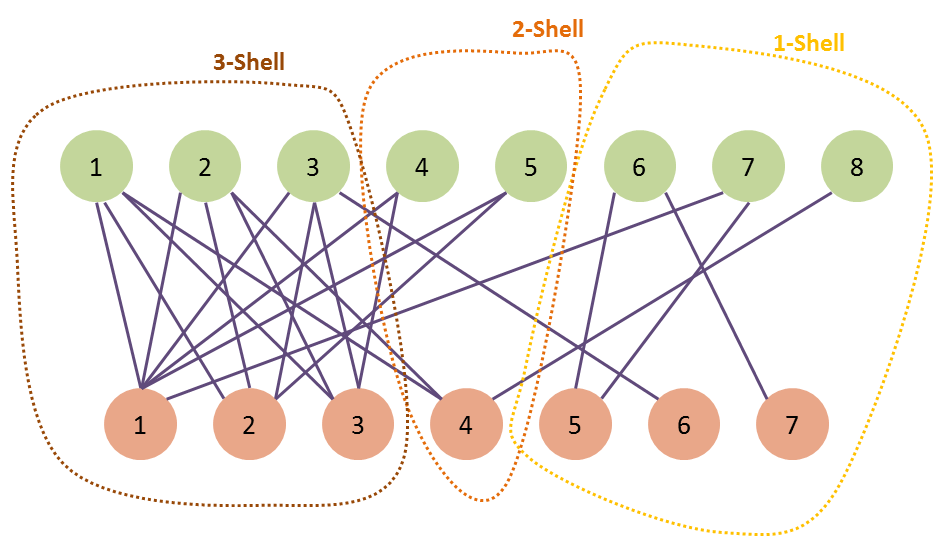
\includegraphics[scale=0.5]{Figures/ESTATICA_kcore_decomposition_example.png}
\caption{Descomposición \textit{k-core} de una red bipartita ficticia.}
\label{fig:ESTATICA_kcore_decomposition_example}
\end{figure}

Según la definición \ref{ESTATICA_def_kcore}, el  \textit{1-core} es la unión de las tres \textit{shell}, mientras que el \textit{2-core} es la unión de la \textit{2-shell} y la \textit{1-shell}. El \textit{k-core} máximo coincide con la  \textit{k-shell} máxima. 

Como estamos tratando de redes bipartitas, distinguimos dos subconjuntos en cada \textit{k-shell}, el de los nodos de la clase $A$ y el de los de la clase $B$. Los llamaremos $K^{A}_{j}, K^{B}_{j}$, donde  $j$ es el índice de la \textit{k-shell}.
Es posible que uno de ellos sea vacío, es decir, no todas las \textit{k-shell} tienen nodos de ambas clases necesariamente.
Al valor máximo de \textit{k}, lo llamamos $ks_{max}$, que corresponde a \textit{shell} más interna de la red $ks_{max}\equiv C^{A,B}$. Esta nomenclatura simplifica la definición de las \textit{k-magnitudes} que surgen de la red descompuesta siguiendo el procedimiento descrito.


\section{K magnitudes}

Las especies más conectadas de una red mutualista son resistentes a las perturbaciones externas porque el beneficio que reciben depende de múltiples fuentes. Esta parece ser la razón por la que las redes mutualistas tienden al anidamiento, una conexión directa con el centro de la red aumenta las probabilidades de supervivencia. Para medir la 'distancia' desde un nodo cualquiera a la \textit{k-shell} más interna de la clase opuesta, hemos definido el \textit{$k_{radius}$}.

\begin{theo} 
El \textit{$k_{radius}$} del nodo $m$ de la clase $A$ es el valor medio de la distancia a las especies de $C^B$
\begin{align*}
\displaystyle
k^A_{radius}m = \frac{1}{\mid C^{B} \mid}\sum\limits_{j \in C^{B}} dist_{mj}  \qquad   m \in A
\stepcounter{equation}\tag{\theequation}\label{kradius}
\end{align*}
\label{ESTATICA_kradius}
\end{theo}

En la fórmula \ref{ESTATICA_kradius} $dist_{mj}$ es el camino más corto de la especie $m$ a cada una de las $j$ especies que forman el conjuto $C^B$. La misma definción es válida para especies de la clase $B$, calculando la distancia media a las especies de $C^A$. El valor mínimo posible de $k_{radius}$ es $1$ para un nodo perteciente a $C^B$ conectado con todas las especies de $C^A$ (y viceversa).

\begin{figure}[h!]
\centering
\includegraphics[scale=0.58]{ESTATICA_red_example.eps}
\caption {Cálculo de \textit{$k_{radius}$} y  \textit{$k_{degree}$} en una red ficticia.}
\label{fig:ESTATICA_red_example}
\end{figure}

La parte superior izquierda de la figura \ref{fig:ESTATICA_red_example} es el esquema de otra red ficticia muy sencilla, con solo siete nodos, tres de la clase $A$ y cuatro de la $B$. Como se puede ver,  la especie $B4$ es la única que pertenece a la $1$-$shell$. El resto son parte de las $2$-$shell$, que por ser la más internas se toman como referencia para medir los $k_{radius}$ individuales. 

En la parte superior derecha de la imagen, se reproduce el detalle de las conexiones de la especie $A1$, perteneciente a $C^{A}$.  Como está directamente conectada con los tres nodos de $C^{B}$ la el camino más corto a cada uno de ellos es $1$, y en consecuencia $k^A_{radius}1$ es $1$. En la parte inferior derecha, la especie $A2$ que también pertenece a $C^{A}$ no tiene enlace directo con $B2$, aunque sí con $B1$ y $B3$. El camino más corto, marcado en color violeta, pasa por $B1$ y $A1$, y mide $3$. El $k^A_{radius}2$ vale $\sfrac{5}{3}$. En la parte inferior izquierda, vemos el esquema de conexiones de la especie $B4$, que no forma parte de $C^{B}$. Como cabía esperar, su$k_{radius}$ es mayor, $\sfrac{7}{3}$. 

Podemos definir una magnitud global, teniendo en cuenta los $k_{radius}$ de todas las especies.

\begin{theo} 
El \textit{$\overline k_{radius}$} de una red se obtiene promediando los ${k}_{radius}$ de todos los nodos, sin importar la clase a la que pertenezcan.
\begin{align*}
\displaystyle
\overline {k}_{radius} = \frac{1}{\mid A \cup B \mid}\sum\limits_{l \in A \cup B} k_{radius}l
\stepcounter{equation}\tag{\theequation}\label{avgkradius}
\end{align*}
\label{ESTATICA_avgkradius}
\end{theo}

Una red con todos sus nodos conectados (matriz de adyacencia cuadrada) tendría $\overline {k}_{radius}=1$, el menor posible. En una con matriz de adyacencia triangular el $\overline {k}_{radius}$ vale $1.5$. En la red que hemos usado como ejemplo, su valor es $\sfrac{11}{7}$. Intuitivamente, el $\overline {k}_{radius}$ será pequeño para redes muy anidadas, porque la probabilidad de conexión con la \textit{shell} más interna es elevada. Las especies generalistas están muy interconectadas y las especialistas tienen enlaces directos con las \textit{k-shells} de mayor índice. por el contrario, una distribución de enlaces puramente aleatoria conduciría a una red con mayor $\overline {k}_{radius}$.

El ${k}_{radius}$ es una buena medida de conexión al corazón de la red pero no de centralidad. Por ejemplo, su valor es bajo para un especialista con un enlace a la \textit{shell} más interna, aunque sabemos que no resulta determinante para la estabilidad global de la red. Para atender esta necesidad, definimos una segunda \textit{k-magnitud}.

\begin{theo} 
\begin{align*}
\displaystyle
k^A_{degree}m = \sum\limits_{j} \frac{a_{mj} }{k_{radius}j}  \quad   m \in A, \forall j \in B
\stepcounter{equation}\tag{\theequation}
\end{align*}
\label{kdegree}
\end{theo}

Donde $a_{mj}$ es el elemento de la matriz de interacción que representa el enlace, cuyo valor es $1$ si existe o $0$ si no está presente. El $k_{degree}$ es la suma de los inversos de los $k_{radius}$ de los nodos conectados con $m$. Una especie de la \textit{shell} más interna tiene un $k_{degree}m$ elevado,  mientras que los especialistas con solo uno o dos enlaces tiene un $k_{degree}$ reducido. Volviendo al ejemplo de la figura \ref{fig:ESTATICA_red_example}, el $k_{degree}$ del nodo $B3$ es is $1+\sfrac{3}{5}+\sfrac{3}{5} = \sfrac{11}{5}$, mientras que solo vale $\sfrac{3}{7}$ para el especialista $B4$. Esta magnitud recuerda la definición del \textit{índice de Harary} \cite{plavvsic1993harary} pero teniendo solo en cuenta los enlaces con la \textit{shell} más interna.


\subsection{Algoritmo de destrucción basado en \textit{k-shell}}

Para poder establecer políticas de conservación es necesario disponer de un respaldo cuantitativo, localizando a las especies que más contribuyen a la estabilidad de las redes \cite{sole2001fragility, dakos2015resilience, thebault2010stability, suweis2013emergence, santamaria2015removing}.  Hay dos aproximaciones posibles. La primera se basa en la dinámica de ponlaciones y depende en gran medida de la parametrización del modelo elegido \cite{dakos2014critical}. La segunda, que utiliza solo la topología de la red, es más sencilla de implementar y por tanto mucho más popular. Es la que seguimos en este capítulo.

La biodiversidad y resistencia de una comunidad mutualista depende de su estructura. La extinción de algunas especies provoca que partes de la red queden desconectadas de la componente gigante y posiblemente expuestas a la desaparición. Por este motivo, la evolución del tamaño de la componente gigante cuando se eliminan especies es el criterio más utilizado para estudiar la resistencia estructural estática.

Esto es lo que hace el método de medida de Dunne \cite{dunne2002biodiversity}, ideado en origen para \textit{food webs}. Las especies se van retirando una por una de la red (extinciones primarias). Este hecho produce extinciones secundarias de aquellas especies. La gráfica de la fracción de la red inicial superviviente, frente a la fracción de extinciones primarias (en escala normalizada entre 0 y 1) define la \textit{curva de extinción}. Cuanto menor sea el área bajo esta curva, más rápida será la destrucción de la red.

\begin{figure}[h!]
\centering
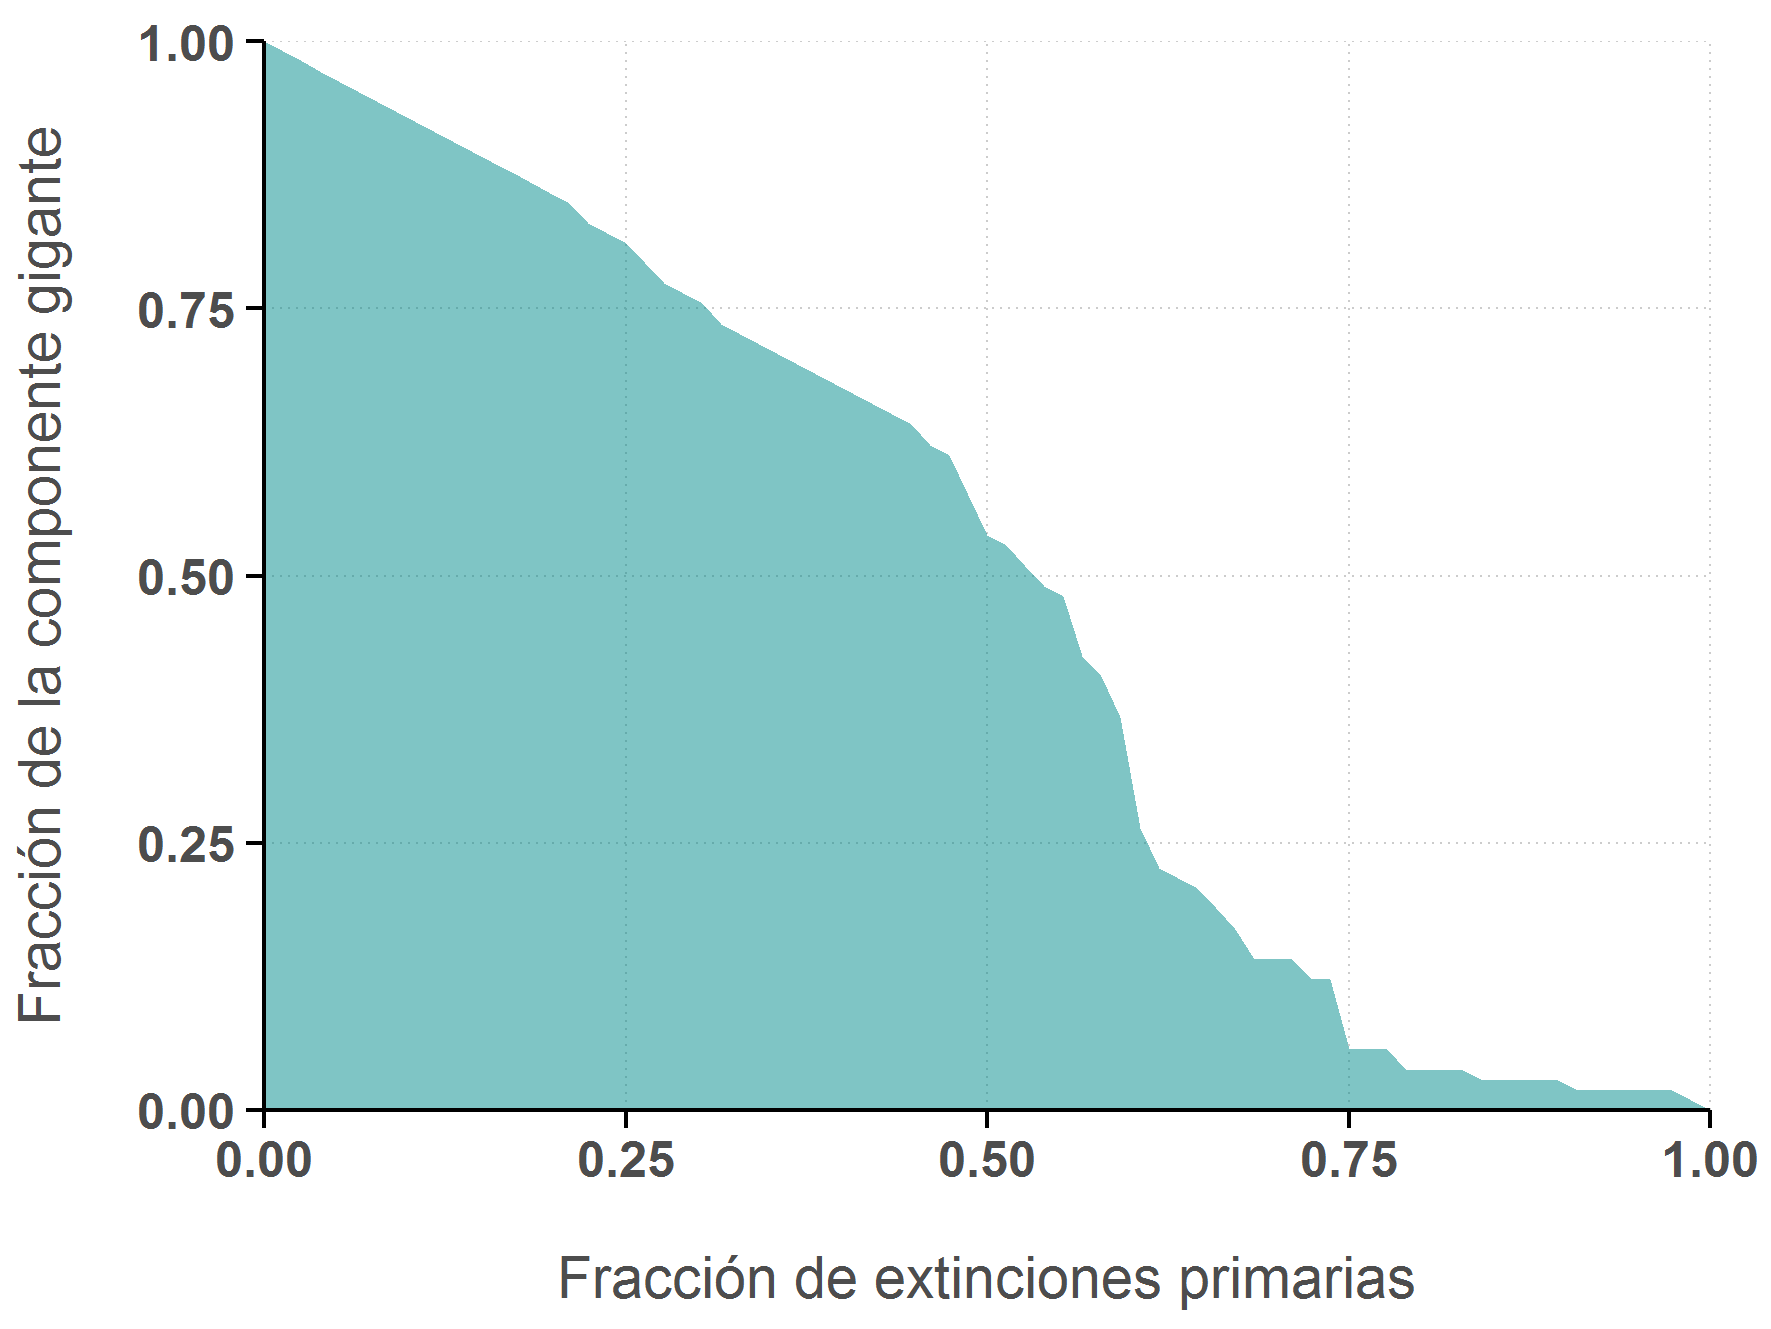
\includegraphics[scale=0.55]{Figures/ESTATICA_destruction_example.png}
\caption{Ejemplo de curva de extinción siguiendo el método de Dunne. El área bajo la curva indica la velocidad a la que se desintegra la componente gigante.}
\label{fig:ESTATICA_destruction_example}
\end{figure}

La clave está en el orden de selección de las especies que se retiran en las extinciones primarias. Si disponemos de una cifra que defina su importancia para esa red concreta, se podrán concentrar los esfuerzos de conservación en las especies que más aportan a la supervivencia del sistema. El problema es que no existe un criterio universalmente aceptado para establecer esa clasificación que resulte óptimo para cualquier red.

En el mutualismo, parece lógico pensar que las especies de las \textit{shells} más internas son las más importantes para mantener la integridad de la red. El algoritmo de destrucción que proponemos se basa en la secuencia $k$-$shell, k_{degree}, k_{radius}$, esto es, se empiezan las extinciones primarias por las especies pertenecientes a la $k$-$shell$ de mayor índice, y dentro de esta, el de mayor $k_{degree}$, y en caso de coincidencia, el de menor $k_{radius}$. 

\section{Material y métodos}

Para este capítulo hemos utilizado la colección de datos de redes mutualistas de la \textit{Web of Life}  \url{http://www.web-of-life.es/} \cite{fortuna2014web}. Hemos analizado todas las disponibles en las categorías \textit{planta-polinizador} y \textit{planta-dispersor de semillas}. En diciembre de 2015 dicha colección consta de 59 redes de la primera familia y 30 de la segunda. El número de especies por red varía entre 6 y 997 y el número de interacciones entre 6 y 2993.

El software se ha desarrollado en \texttt{R} y \texttt{Python}. La \textit{descomposición k-core} se realiza con el paquete \texttt{R} \texttt{igraph} \cite{csardi2006igraph}. El mismo paquete ofrece funciones para el cálculo de $NODF$ y $Modularity$. El código \texttt{R} para medir ${k}_{degree}$ y ${k}_{radius}$ es propio. Los valores medios de estas magnitudes se calculan descartando las especies que no pertenecen a la componente gigante cuando en la red se produce esta circunstancia. 

Para medir la bondad del algoritmo de destrucción, hemos comparado su rendimiento con el que ofrece \textit{MusRank}, de reciente publicación y basado en una clasificación de la importancia de los nodos similar a la del \textit{PageRank} de Google  \citep{dominguez2015ranking}. Tanto el algoritmo basado en \textit{k-shell} como la medición del \textit{MusRank} se han codificado en \texttt{Python}.

\begin{table}[htbp]
\tiny
  \centering
    \begin{tabular}{lrrrrrrrrr}
    \toprule
    $Red$  & $Plantas$ & $Animales$ & $Enlaces$ & $k_{max}$ & $\overline k_{degree}$ & $\overline k_{radius}$ & $NODF$ & $Modularity$ & $Area_{Mus-k}$ \\
    \midrule
 
    M\_PL\_001 & 84   & 101  & 361  & 4    & 1,56 & 3,01 & 14,46 & 0,45 & 0,08 \\
    M\_PL\_002 & 43   & 64   & 196  & 3    & 1,4  & 3,04 & 15,36 & 0,48 & 0,11 \\
    M\_PL\_003 & 36   & 25   & 81   & 2    & 0,93 & 3,31 & 19,19 & 0,57 & 0,02 \\
    M\_PL\_004 & 12   & 102  & 167  & 3    & 1,52 & 2,53 & 28,15 & 0,45 & 0,09 \\
    M\_PL\_005 & 96   & 275  & 923  & 8    & 2,54 & 2,8  & 14,74 & 0,24 & 0,14 \\
    M\_PL\_006 & 17   & 61   & 146  & 4    & 2,28 & 2,44 & 44,58 & 0,33 & 0,04 \\
    M\_PL\_007 & 16   & 36   & 85   & 3    & 1,68 & 2,51 & 31,54 & 0,36 & 0,12 \\
    M\_PL\_008 & 11   & 38   & 106  & 4    & 2,19 & 2,37 & 35,97 & 0,21 & 0,03 \\
    M\_PL\_009 & 24   & 118  & 242  & 4    & 1,54 & 2,81 & 15,39 & 0,44 & 0,16 \\
    M\_PL\_010 & 31   & 76   & 456  & 8    & 4,57 & 2,38 & 35,17 & 0,02 & 0,03 \\
    M\_PL\_011 & 14   & 13   & 52   & 3    & 2,27 & 2,16 & 54,59 & 0,29 & 0 \\
    M\_PL\_012 & 29   & 55   & 145  & 4    & 2,01 & 2,51 & 30,4 & 0,42 & 0,05 \\
    M\_PL\_013 & 9    & 56   & 103  & 4    & 1,96 & 2,4  & 34,25 & 0,38 & 0,14 \\
    M\_PL\_014 & 29   & 81   & 179  & 3    & 1,48 & 2,8  & 25,68 & 0,44 & 0,08 \\
    M\_PL\_015 & 131  & 666  & 2933 & 9    & 2,9  & 2,88 & 9,17 & 0,35 & 0,08 \\
    M\_PL\_016 & 26   & 179  & 412  & 5    & 1,88 & 2,73 & 21,98 & 0,42 & 0,15 \\
    M\_PL\_017 & 25   & 79   & 299  & 6    & 3,28 & 2,47 & 40,37 & 0,15 & 0,04 \\
    M\_PL\_018 & 39   & 105  & 383  & 5    & 2,26 & 2,74 & 19,73 & 0,24 & 0,11 \\
    M\_PL\_019 & 40   & 85   & 264  & 5    & 1,97 & 2,71 & 17,51 & 0,34 & 0,13 \\
    M\_PL\_020 & 20   & 91   & 190  & 4    & 1,84 & 2,56 & 37,12 & 0,39 & 0,09 \\
    M\_PL\_021 & 91   & 677  & 1193 & 5    & 1,23 & 3,06 & 7,55 & 0,58 & 0,21 \\
    M\_PL\_022 & 21   & 45   & 83   & 2    & 0,84 & 3,68 & 18,02 & 0,6  & 0,14 \\
    M\_PL\_023 & 23   & 72   & 125  & 3    & 1,35 & 2,75 & 22,88 & 0,54 & 0,14 \\
    M\_PL\_024 & 11   & 18   & 38   & 3    & 1,71 & 1,97 & 29,02 & 0,42 & 0,16 \\
    M\_PL\_025 & 13   & 44   & 143  & 5    & 3,4  & 2,13 & 46,02 & 0,16 & 0 \\
    M\_PL\_026 & 105  & 54   & 204  & 3    & 1,13 & 2,85 & 25,13 & 0,56 & 0,11 \\
    M\_PL\_027 & 18   & 60   & 120  & 3    & 1,2  & 2,96 & 13,94 & 0,55 & 0,19 \\
    M\_PL\_028 & 41   & 139  & 374  & 5    & 2,11 & 2,75 & 16,43 & 0,37 & 0,1 \\
    M\_PL\_029 & 49   & 118  & 346  & 5    & 1,94 & 2,76 & 15,77 & 0,41 & 0,12 \\
    M\_PL\_030 & 28   & 53   & 109  & 2    & 0,83 & 3,54 & 11,16 & 0,54 & 0,17 \\
    M\_PL\_031 & 48   & 49   & 156  & 4    & 1,57 & 3,39 & 12,34 & 0,54 & 0,05 \\
    M\_PL\_032 & 7    & 33   & 65   & 3    & 2,41 & 2,07 & 56,66 & 0,1  & 0,05 \\
    M\_PL\_033 & 13   & 34   & 141  & 5    & 3,4  & 2,24 & 29,5 & 0,07 & 0,04 \\
    M\_PL\_034 & 26   & 128  & 312  & 5    & 2,1  & 2,61 & 25,01 & 0,42 & 0,08 \\
    M\_PL\_035 & 61   & 36   & 178  & 4    & 1,74 & 2,85 & 25,74 & 0,43 & 0 \\
    M\_PL\_036 & 10   & 12   & 30   & 2    & 1,31 & 2,51 & 35,96 & 0,38 & 0,09 \\
    M\_PL\_037 & 10   & 40   & 72   & 3    & 1,37 & 2,7  & 23,16 & 0,44 & 0,14 \\
    M\_PL\_038 & 8    & 42   & 79   & 3    & 1,56 & 2,44 & 28,31 & 0,39 & 0,06 \\
    M\_PL\_039 & 17   & 51   & 129  & 4    & 1,99 & 2,61 & 25,34 & 0,45 & 0,12 \\
    M\_PL\_040 & 29   & 43   & 114  & 3    & 1,32 & 2,92 & 15,18 & 0,5  & 0,03 \\
    M\_PL\_041 & 31   & 43   & 145  & 4    & 2,11 & 2,51 & 25,3 & 0,35 & 0,11 \\
    M\_PL\_042 & 12   & 6    & 25   & 3    & 2,34 & 1,71 & 49,79 & 0,33 & 0,07 \\
    M\_PL\_043 & 28   & 82   & 250  & 4    & 1,99 & 2,71 & 22,17 & 0,29 & 0,1 \\
    M\_PL\_044 & 110  & 609  & 1125 & 4    & 1,12 & 3,36 & 4,92 & 0,57 & 0,22 \\
    M\_PL\_045 & 17   & 26   & 63   & 3    & 1,73 & 2,43 & 30,77 & 0,45 & 0,09 \\
    M\_PL\_046 & 16   & 44   & 278  & 8    & 6,45 & 1,96 & 63,6 & -0,03 & 0 \\
    M\_PL\_047 & 19   & 186  & 425  & 6    & 2,31 & 2,56 & 29,96 & 0,29 & 0,09 \\
    M\_PL\_048 & 30   & 236  & 671  & 7    & 2,78 & 2,61 & 26,23 & 0,21 & 0,08 \\
    M\_PL\_049 & 37   & 225  & 590  & 6    & 2,08 & 2,76 & 18,13 & 0,38 & 0,14 \\
    M\_PL\_050 & 14   & 35   & 86   & 3    & 1,71 & 2,49 & 32,58 & 0,43 & 0,08 \\
    M\_PL\_051 & 14   & 90   & 164  & 4    & 2,13 & 2,34 & 26,96 & 0,45 & 0,1 \\
    M\_PL\_052 & 15   & 39   & 92   & 3    & 1,7  & 2,51 & 30,91 & 0,31 & 0,14 \\
    M\_PL\_053 & 99   & 294  & 589  & 3    & 0,92 & 3,8  & 4,71 & 0,58 & 0,2 \\
    M\_PL\_054 & 113  & 318  & 773  & 5    & 1,42 & 3,07 & 8,08 & 0,46 & 0,2 \\
    M\_PL\_055 & 64   & 195  & 431  & 4    & 1,29 & 3,13 & 8,71 & 0,52 & 0,19 \\
    M\_PL\_056 & 91   & 365  & 871  & 5    & 1,43 & 3,24 & 6,86 & 0,46 & 0,17 \\
    M\_PL\_057 & 114  & 883  & 1920 & 8    & 1,8  & 2,88 & 7,04 & 0,48 & 0,23 \\
    M\_PL\_058 & 32   & 81   & 319  & 6    & 3,03 & 2,48 & 26,64 & 0,22 & 0,06 \\
    M\_PL\_059 & 13   & 13   & 71   & 5    & 4,72 & 1,57 & 76,88 & 0,04 & 0,01 \\
    M\_SD\_001 & 7    & 21   & 50   & 3    & 2,33 & 2,16 & 40,77 & 0,18 & 0,06 \\
    M\_SD\_002 & 31   & 9    & 119  & 6    & 4,61 & 1,85 & 62,16 & 0,02 & -0,02 \\
    M\_SD\_003 & 25   & 16   & 68   & 3    & 1,78 & 2,45 & 41,09 & 0,33 & 0,05 \\
    M\_SD\_004 & 34   & 20   & 95   & 4    & 2,37 & 2,19 & 39,82 & 0,35 & 0,01 \\
    M\_SD\_005 & 25   & 13   & 49   & 3    & 1,33 & 2,38 & 27,93 & 0,53 & 0,1 \\
    M\_SD\_006 & 21   & 15   & 51   & 3    & 1,51 & 2,35 & 32,79 & 0,45 & 0,08 \\
    M\_SD\_007 & 72   & 7    & 143  & 3    & 2,34 & 2,37 & 51,67 & 0,28 & 0 \\
    M\_SD\_008 & 16   & 10   & 110  & 7    & 6,56 & 1,48 & 56,33 & -0,04 & -0,01 \\
    M\_SD\_009 & 7    & 18   & 38   & 3    & 1,9  & 2,15 & 33,02 & 0,32 & 0,06 \\
    M\_SD\_010 & 50   & 14   & 234  & 6    & 4,48 & 2,14 & 42,13 & 0,04 & -0,1 \\
    M\_SD\_011 & 11   & 14   & 47   & 3    & 2,14 & 2,17 & 45,41 & 0,31 & 0,03 \\
    M\_SD\_012 & 35   & 29   & 146  & 4    & 2,31 & 2,57 & 33,04 & 0,23 & 0 \\
    M\_SD\_013 & 36   & 19   & 197  & 7    & 4,38 & 2,31 & 37,37 & 0,33 & -0,13 \\
    M\_SD\_014 & 16   & 17   & 121  & 5    & 5,16 & 1,87 & 78,76 & 0,08 & -0,01 \\
    M\_SD\_015 & 5    & 27   & 86   & 4    & 4,25 & 1,65 & 67,34 & 0,03 & -0,01 \\
    M\_SD\_016 & 24   & 61   & 500  & 11   & 8,4  & 2,01 & 58,84 & 0    & 0,01 \\
    M\_SD\_017 & 16   & 8    & 72   & 5    & 4,74 & 1,63 & 60,12 & 0,08 & -0,04 \\
    M\_SD\_018 & 29   & 32   & 66   & 2    & 0,75 & 3,41 & 11,21 & 0,59 & 0,21 \\
    M\_SD\_019 & 169  & 40   & 666  & 7    & 3,23 & 2,62 & 32,87 & 0,33 & -0,09 \\
    M\_SD\_020 & 25   & 33   & 150  & 5    & 3,07 & 2,31 & 53,55 & 0,13 & -0,01 \\
    M\_SD\_021 & 18   & 28   & 129  & 5    & 3,46 & 2,19 & 61,52 & 0,18 & -0,01 \\
    M\_SD\_022 & 207  & 110  & 1121 & 8    & 3,21 & 2,8  & 16,81 & 0,2  & -0,01 \\
    M\_SD\_023 & 15   & 8    & 38   & 3    & 2,3  & 2,03 & 66,8 & 0,22 & 0 \\
    M\_SD\_024 & 12   & 7    & 40   & 3    & 2,5  & 1,99 & 56,83 & 0,12 & -0,02 \\
    M\_SD\_025 & 7    & 6    & 22   & 3    & 2,41 & 1,69 & 66,67 & 0,19 & 0 \\
    M\_SD\_026 & 3    & 3    & 6    & 2    & 1,83 & 1,33 & 100  & 0,17 & 0 \\
    M\_SD\_027 & 12   & 4    & 31   & 4    & 3,45 & 1,53 & 73,61 & 0    & 0 \\
    M\_SD\_028 & 8    & 5    & 26   & 4    & 3,65 & 1,38 & 89,47 & 0,02 & 0 \\
    M\_SD\_029 & 4    & 5    & 10   & 2    & 1,98 & 1,52 & 81,25 & 0,27 & 0 \\
    M\_SD\_030 & 5    & 4    & 11   & 2    & 2,24 & 1,5  & 66,67 & 0,23 & 0 \\
    
    \bottomrule
    \end{tabular}%
    \caption{\label{table:table_results} Propiedades de las redes utilizadas en el estudio.}

\end{table}%

\section{Resultados}

En este apartado se describen los resultados de los siguientes procedimientos: análisis exploratorio de los datos de las redes de la colección, estudio de la correlación entre las \textit{k-magnitudes} las medidas estadísticas habituales, experimento de recableado y comparación del algoritmo de destrucción basado en \textit{k-shell} con el basado en \textit{MusRank}.

\subsection{Análisis exploratorio}

En la figura \ref{fig:ESTATICA_hist_kmagnitudes} se han representado los histogramas de las tres \textit{k-magnitudes} que describen globalmente las redes incluidas en la investigación. En la mitad de ellas el índice $k$ máximo es $4$ o menos y solo hay dos que tengan más de $8$. La distribución del $\overline{k}_{radius}$ es aproximadamente normal, con una mediana de $2,51$ y media $2,47$. Teniendo en cuenta que el valor mínimo de esta magnitud es $1$, podemos deducir que las redes mutualistas analizadas son \textit{very small world}, las especies se encuentran muy próximas a la \textit{k-shell} más interna. Este dato concuerda con la observación de que los especialistas se conectan con generalistas lo que les proporciona más probabilidades de supervivencia. Finalmente, el $\overline{k}_{degree}$ se
concentra entre los valores $0,5$ y $3,5$ con la mediana en $2,08$. La conectividad media de las redes es reducida
porque abundan los especialistas. En el tercer histograma hay una diferencia sensible entre las redes de polinizadores
y las de dispersores de semillas, pues estas últimas tienen valores más elevados.

\begin{figure}[h!]
\centering
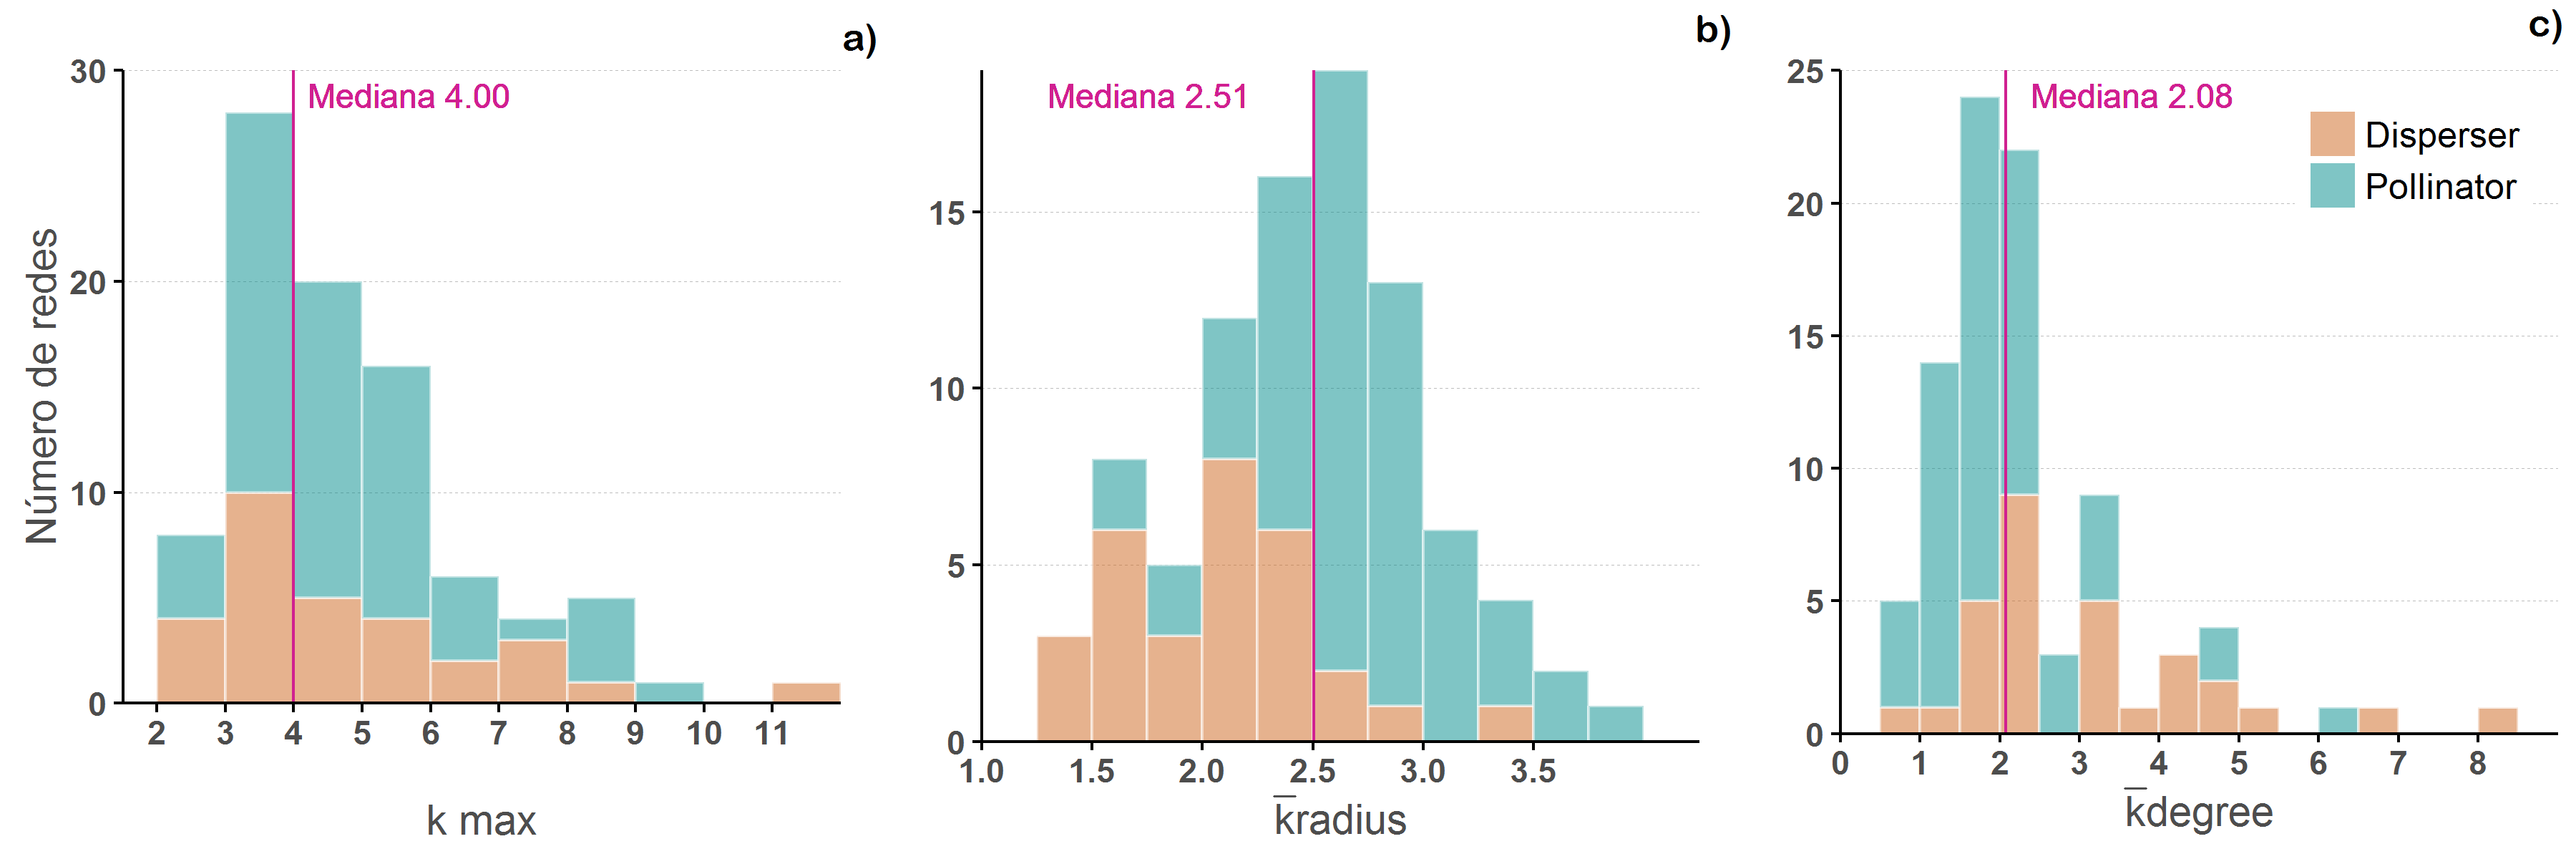
\includegraphics[scale=0.5]{Figures/ESTATICA_hist_kmagnitudes.png}
\caption{Histogramas de las \textit{k-magnitudes}.}
\label{fig:ESTATICA_hist_kmagnitudes}
\end{figure}

En una primera aproximación visual a los datos, encontramos que existía una alta correlación entre el $\overline{k}_{radius}$ de la red y el número de especies (figura \ref{fig:ESTATICA_tamanyo_kdegree_kradius}). Como cabía esperar, cuanto mayor es la red, mayor es la distancia media a la \textit{shell} máxima. El crecimiento sigue una ley logarítmica, nótese la escala del eje $X$. Sucede algo parecido con el número de enlaces, pero en este caso se puede apreciar mayor dispersión. 

Por el contrario, el $\overline{k}_{degree}$ no parece guardar ninguna relación con el tamaño de la red, ya se mida en número total de especies o de enlaces. Vemos que para la mayoría de redes su valor está en torno a $2$. Este dato hace sospechar que la distribución del ${k}_{degree}$ en las redes sigue una exponencial decreciente. La mayoría de los nodos tienen valores bajos, por lo que la media arroja ese valor tan pequeño. En la figura \ref{fig:ESTATICA_density_plots} aparecen las gráficas de dicha distribución de tres redes en las que resulta evidente la asimetría. 

\begin{figure}[h!]
\centering
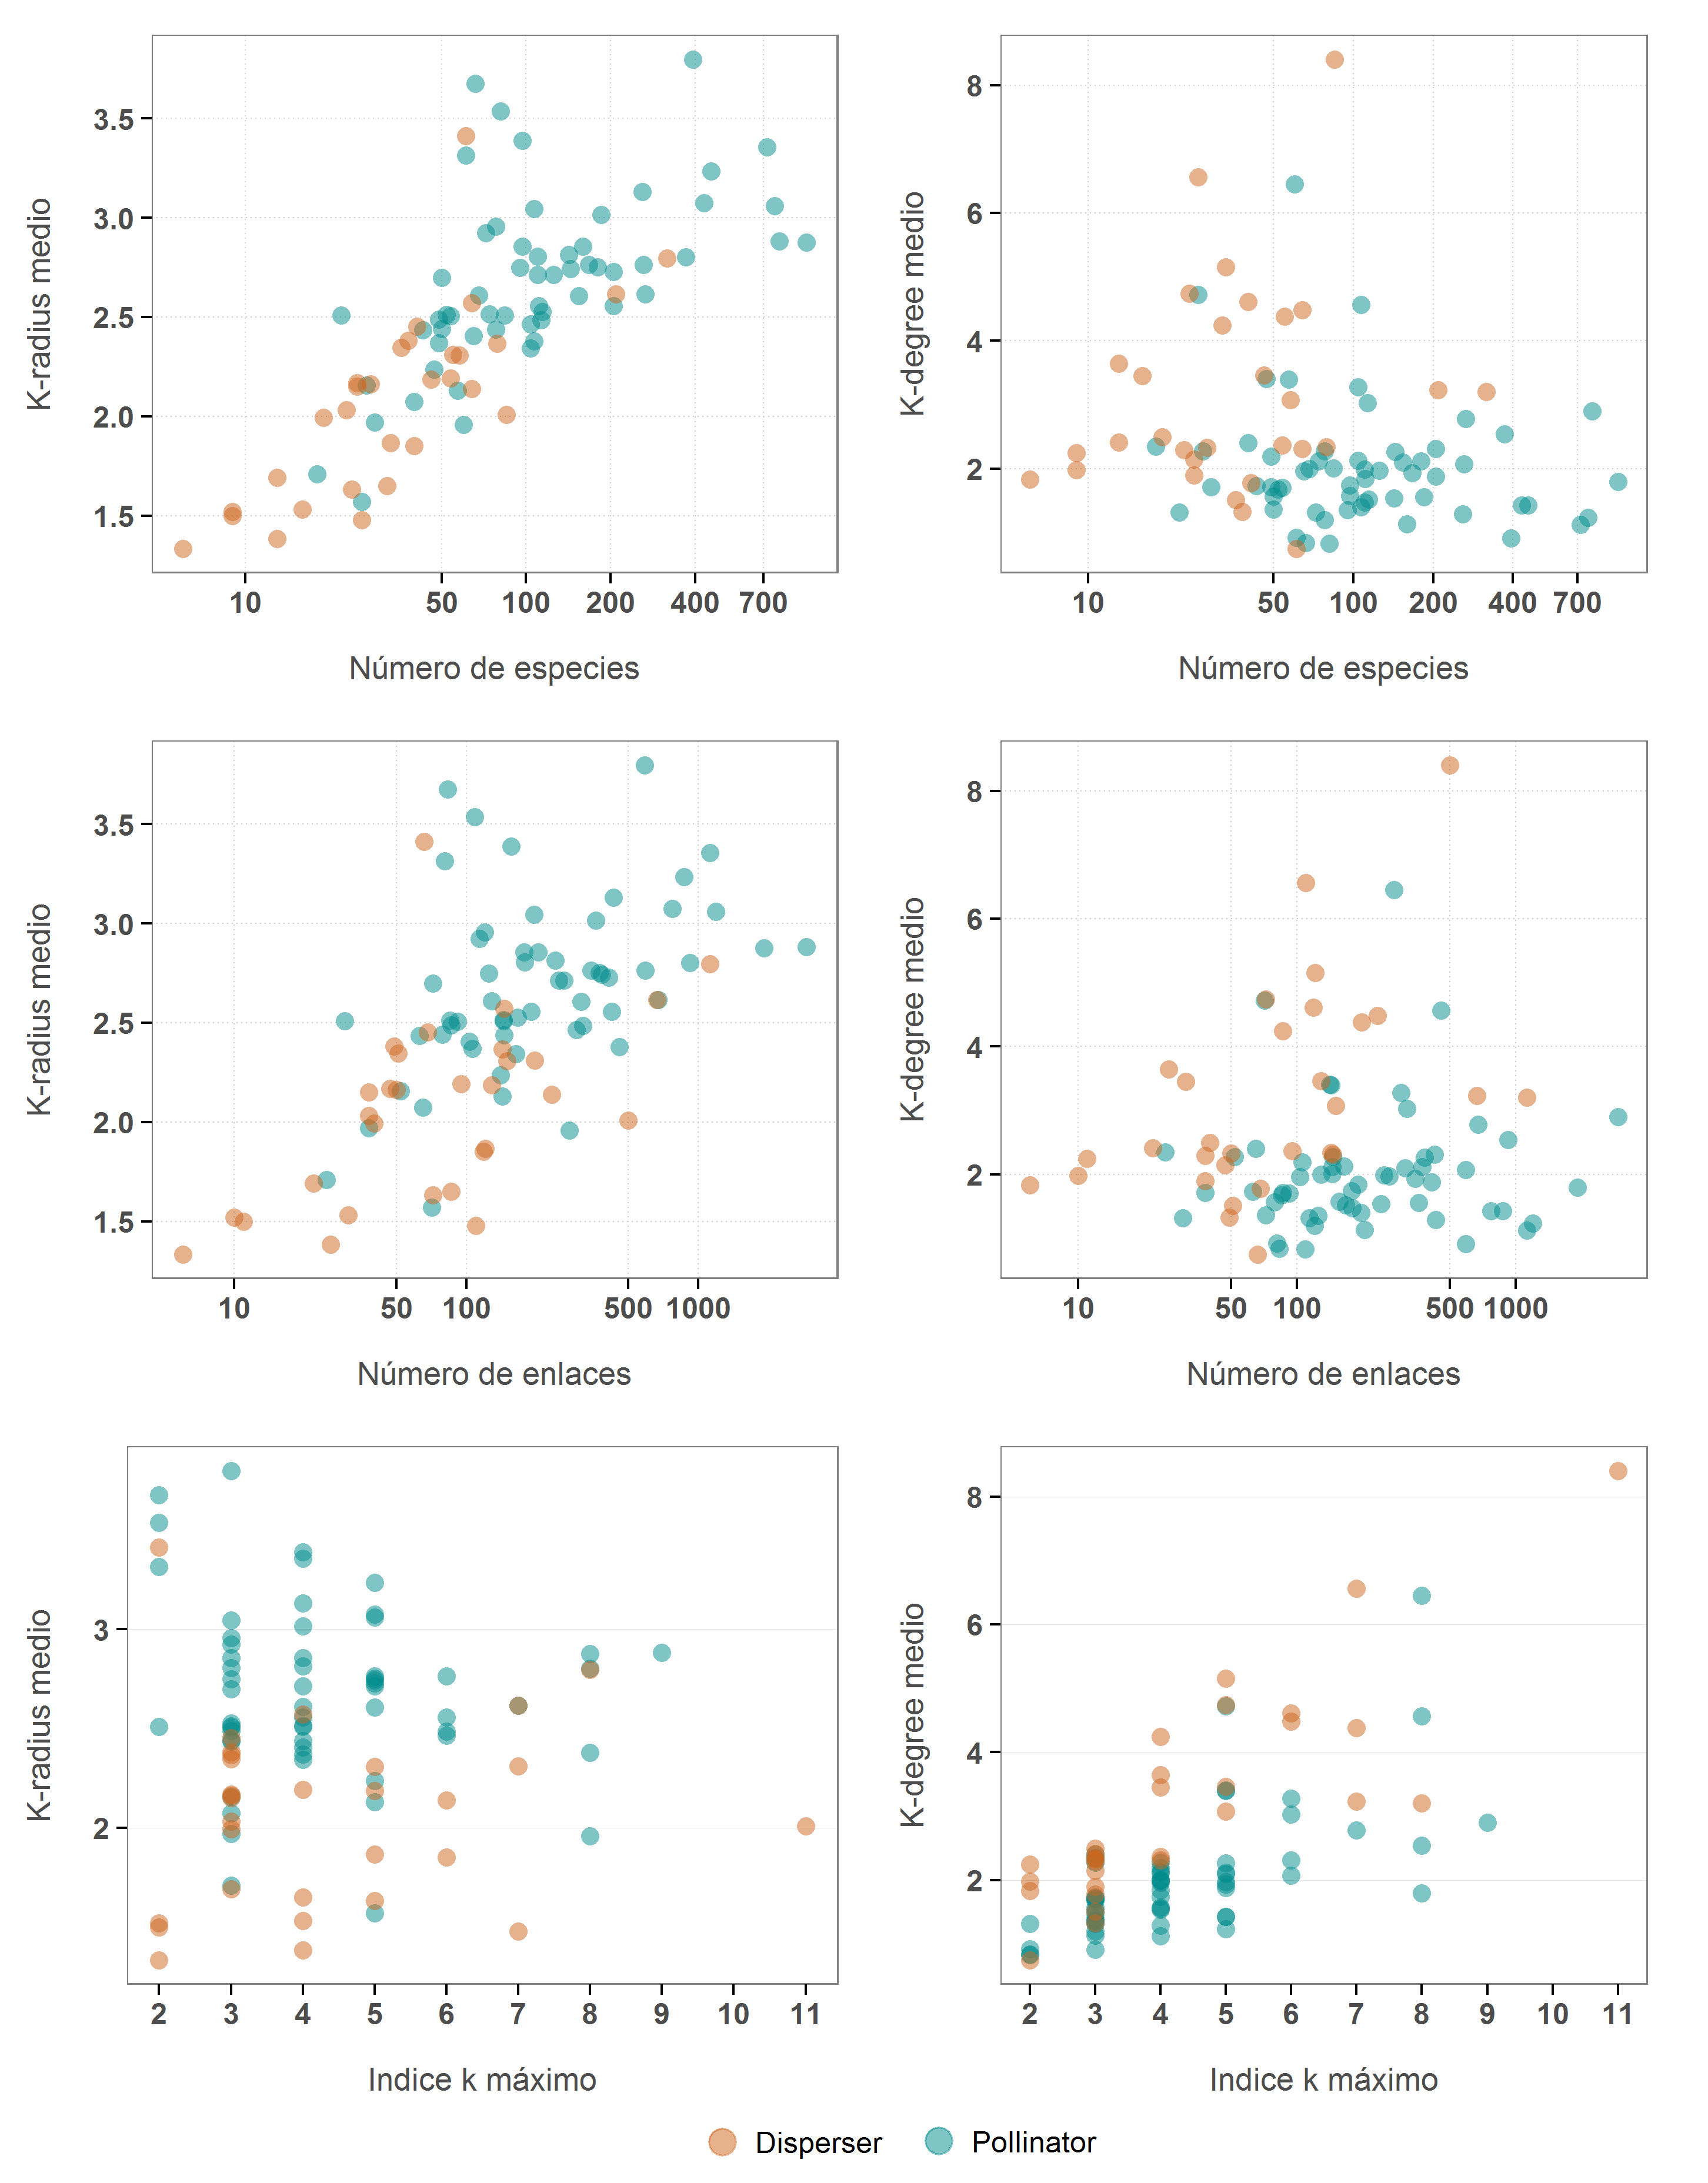
\includegraphics[scale=0.18]{Figures/ESTATICA_tamanyo_kdegree_kradius.png}
\caption{Diagramas de dispersión que relacionan las \textit{k-magnitudes} con el tamaño de la red.}
\label{fig:ESTATICA_tamanyo_kdegree_kradius}
\end{figure}

Si observamos la relación entre las dos \textit{k-magnitudes} y el indíce $k$ máximo de la red, descubrimos que la relación es inversa, el $\overline{k}_{degree}$ crece con el índice y el $\overline{k}_{radius}$ disminuye. No obstante, se aprecia una importante dispersión para redes con un mismo $k$ máximo.


\subsection{Correlación entre \textit{k-magnitudes} y propiedades globales}

Uno de los objetivos principales de la investigación es hallar la posible relación entre las magnitudes que se derivan de la \textit{descomposición k-core} y las que se utilizan habitualmente en la caracterización del mutualismo. Hemos encontrado que las \textit{k-magnitudes} globales tienen una fuerte correlación con estas dos medidas, y esto es de gran interés puesto que surgen de la agregación de las propiedades locales de cada nodo.

Para realizar la comparación se calcula el anidamiento mediante \textit{NODF} y la modularidad siguiendo la definición de \textit{Modularity} de Newman \cite{almeida2008consistent, newman2004finding} \footnote{Para evitar confusiones entre el nombre la de la magnitud y la medida según un algoritmo concreto, en lo sucesivo se emplea \textit{Modularity}, en inglés y con mayúscula, para referirse al valor definido por Newman.}. Ambas medidas las proporciona el paquete \texttt{bipartite} en \texttt{R}. En la figura \ref{fig:ESTATICA_corrfigs} se han representado el $\overline {k}_{radius}$ en función de $NODF$ y el $\overline {k}_{degree}$ en función de la $modularidad$. Las figuras sugerían que existe un fuerte correlación negativa entre el $\overline {k}_{radius}$ y $NODF$ por una parte y, por otra, entre el $\overline {k}_{degree}$ y la $modularidad$. 

\begin{figure}[h!]
\centering
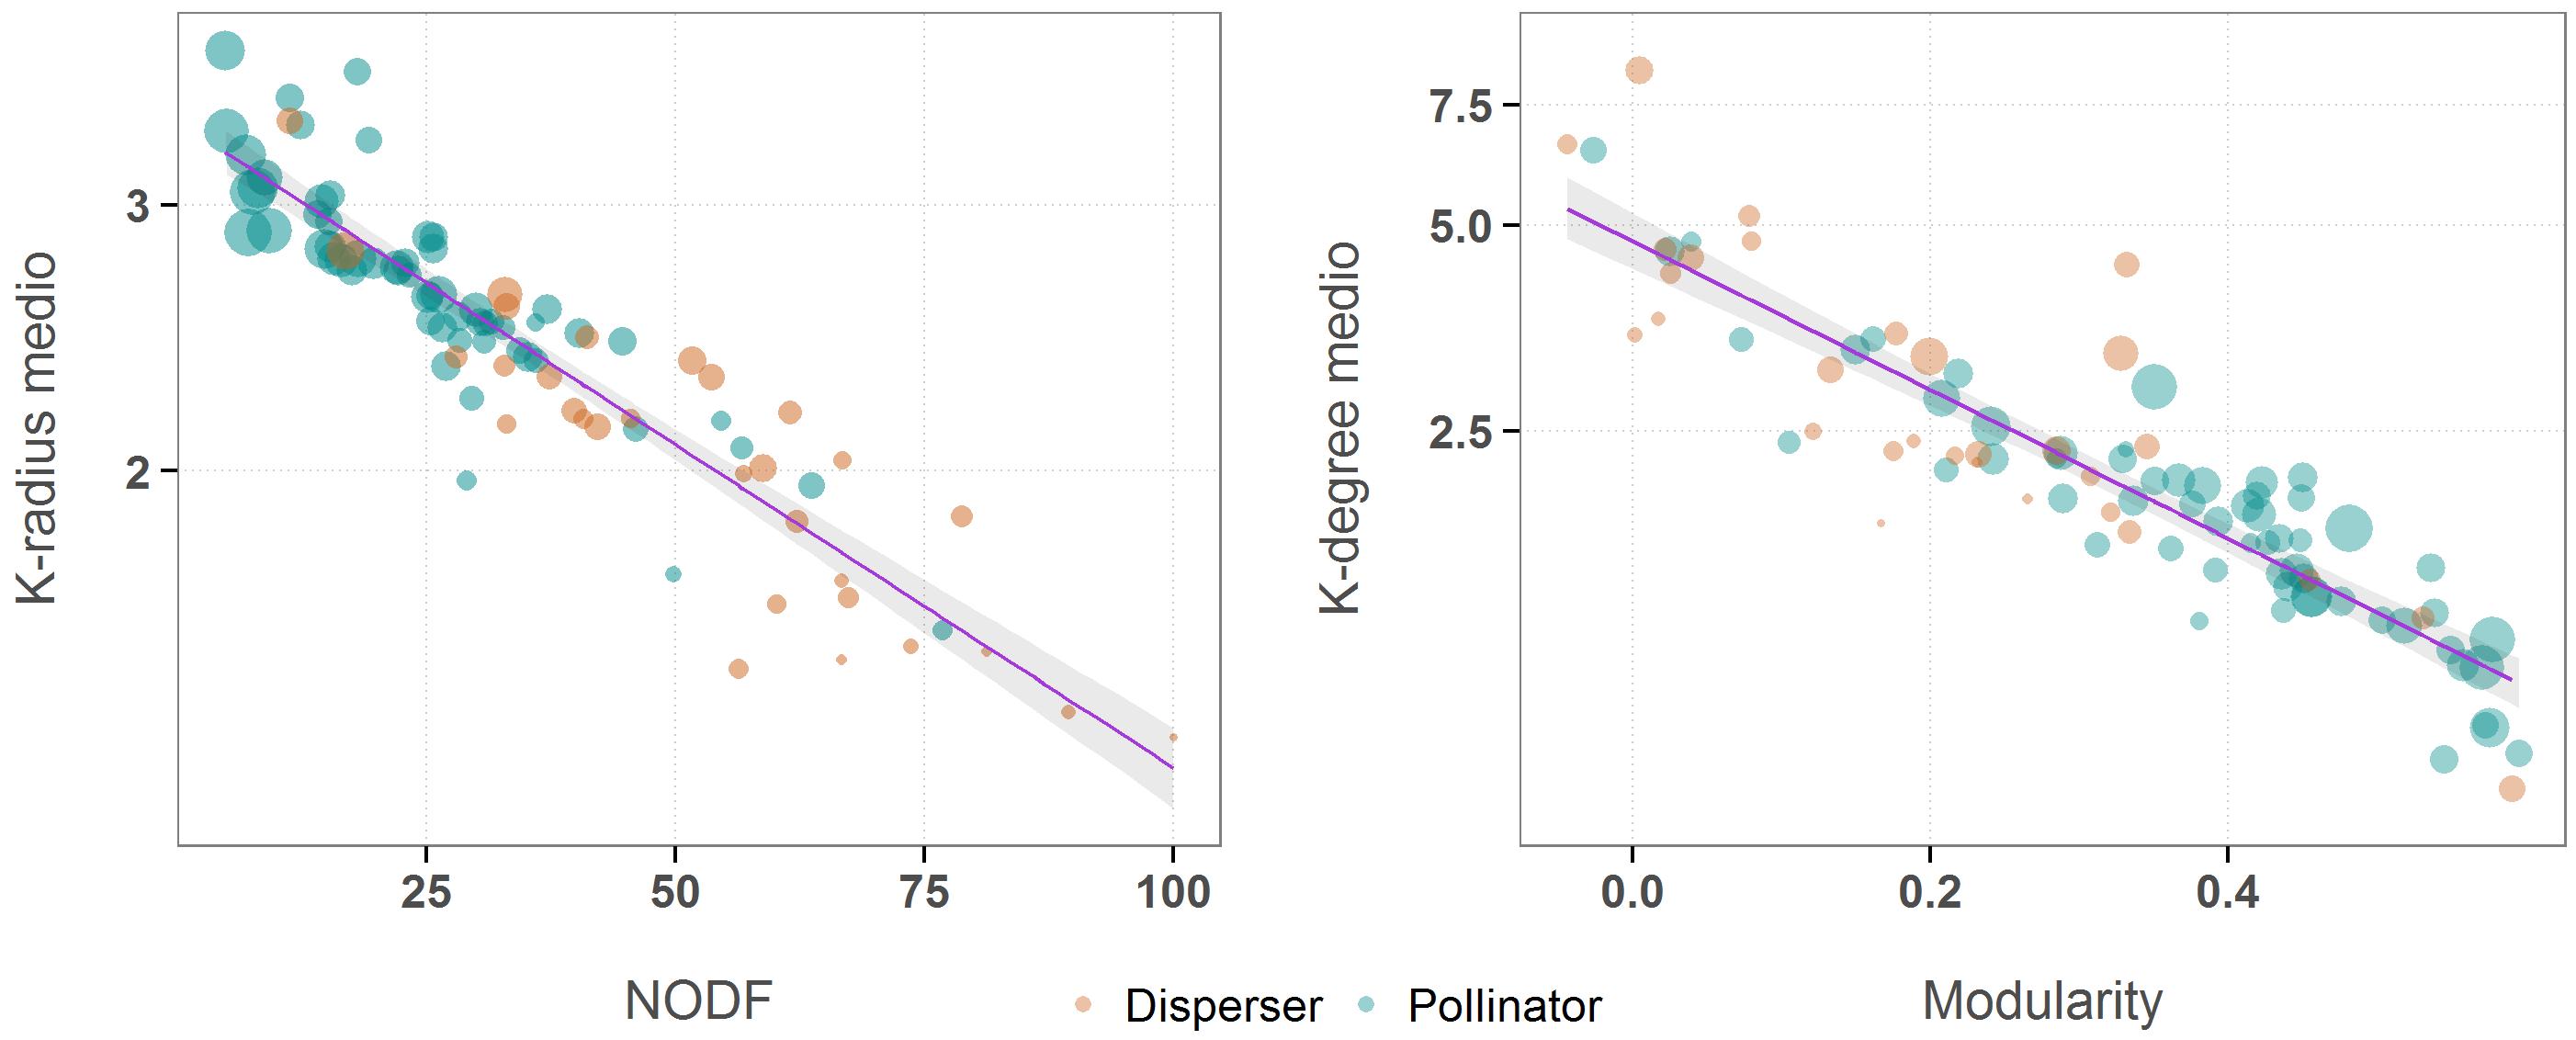
\includegraphics[scale=0.2]{ESTATICA_correlation_figs.png}
\caption {Diagrama de dispersión del $\overline {k}_{radius}$ respecto a $NODF$ (izquierda), y del $\overline {k}_{degree}$ respecto a la $Modularity$ (derecha). Cada punto es una red, su área es proporcional al logaritmo del número de especies y el color indica la clase de comunidad. Se han incluido las líneas de regresión con sus intervalos de confianza en sombreado.}
\label{fig:ESTATICA_corrfigs}
\end{figure}

Las nubes de puntos se representan sobre eje lineal en las abscisas y logarítmico en las ordenadas. Parecen compatibles con un modelo exponencial, así que procedimos a calcular las regresiones lineales $log(Y) ~ X$. Los resultados numéricos se resumen en la tabla \ref{table:table_lmodel}. Como muestra el valor ajustado de $R^2$ $(0,84)$, el logaritmo de $\overline {k}_{radius}$ tiene una correlación muy elevada con $NODF$. 
\begin{align}
\displaystyle \log({\overline k_{radius}}) = \beta_1 \times NODF + \beta_0
\stepcounter{equation}\tag{\theequation}\label{eq:kradius_vs_nodf}
\end{align}
Es sencillo de entender; si la red es muy anidada las especies se conectan directamente a las \textit{shells} más internas y su distancia a los nodos de la \textit{shell} máxima es pequeña. 

\begin{table}[ht]
\centering
\begin{tabular}{|l r | l r|}
\hline
$log(\overline {k}_{radius})$ vs $NODF$& & $log(\overline {k}_{degree})$ vs $Modularity$ & \\
\hline
$\beta_1$ & $-$0.0098 & $\beta'_1$ & -2.5031 \\
$\beta_0$ & 1.2269 & $\beta'_0$ & 1.5553 \\
$R^2$ ajustado&  0.8427  & $R'^2$ ajustado& 0.8064\\
p-value & $<2.2 \times 10^{-16}$& p-value' & $<2.2 \times 10^{-16}$\\
\hline
\end{tabular}
\caption{\label{table:table_lmodel} Resultados de las regresiones lineales}
\end{table}

La correlación entre $\overline {k}_{degree}$ y $Modularity$ es más complicada de intuir. La distribución de densidad del $k_{degree}$ está más concentrada y sesgada hacia la izquierda cuanto más modular es la red. En ese caso la mayoría de las especies tienen valores reducidos del ${k}_{degree}$ y en consecuencia el valor medio es reducido. La distribución se va aplanando a medida que la modularidad decrece y el valor medio se desplaza hacia la derecha. En la figura \ref{fig:ESTATICA_density_plots} se puede ver este efecto.

Si se examina de nuevo la figura \ref{fig:ESTATICA_corrfigs}, se verá que las redes de mayor tamaño son también las que tienen valores más altos de $Modularity$. La mayoría de ellas son de la clase \textit{planta-polinizador} mientras que las tipo \textit{dispersor de semillas} son más pequeñas. Este hecho ya fue puntado por Olesen que estudió 51 redes y encontró que las que tienen menos de 150 especies no son modulares \cite{olesen2007modularity}. Los valores elevados de $\overline {k}_{degree}$ en redes reducidas casan bien con la observación de que en ese caso las especies se encuentran más próximas a la \textit{shell} más interna y añaden valores altos al ${k}_{degree}$ de las especies a las que se conectan.

\begin{figure}[h!]
\centering
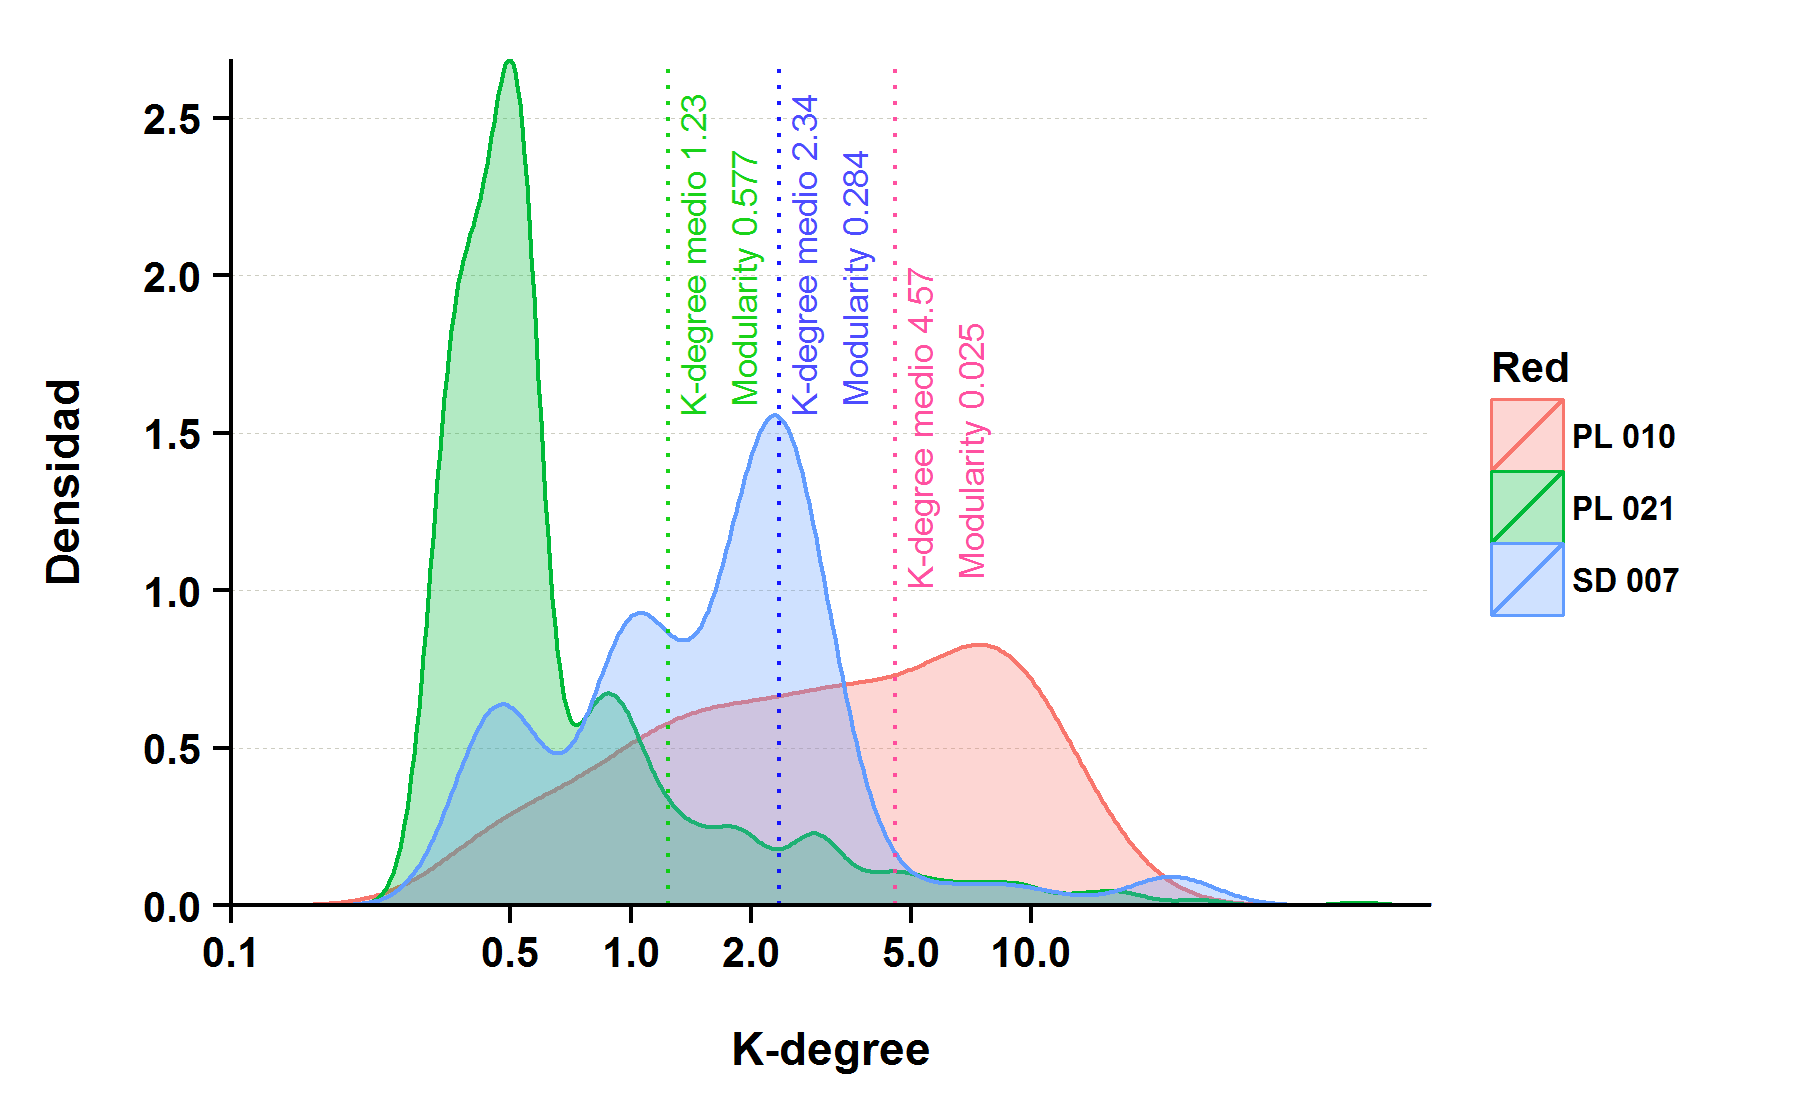
\includegraphics[scale=0.85]{ESTATICA_density_plots.png}
\caption {Distribución de densidad del $k_{degree}$ en tres redes diferentes. Junto a las líneas verticales pueden verse los valores del $\overline {k}_{degree}$ y de la $Modularity$.}
\label{fig:ESTATICA_density_plots}
\end{figure}

Las elevadas correlaciones de $\overline {k}_{radius}$ con $NODF$ y de $\overline {k}_{radius}$ con $Modularity$ son suficientes para esta investigación. Por ejemplo, no se propugna que $log(\overline {k}_{radius})$ sea un buen predictor de $NODF$, de hecho el test de \textit{Shapiro-Wilk} muestra heterocedasticidad. La colección de la \textit{Web of Life} no es una muestra aleatoria, y la distribución de las magnitudes no son normales. Sin embargo, las correlaciones apoyan la idea de que el $\overline {k}_{radius}$ es un indicador global de anidamiento, y el $\overline {k}_{degree}$ de modularidad y que la \textit{descomposición k-core} es una alternativa válida para el estudio del mutualismo.

\subsection{Recableado aleatorio}

Con este experimento se busca entender como se alteran $\overline {k}_{radius}$ y $NODF$ al reconectar al azar un porcentaje de enlaces de la red. La idea subyacente es que las comunidades mutualistas adoptan configuraciones estables, con anidamiento fuerte y $\overline {k}_{radius}$ reducido. Si esto es así, el recableado debe de conducir a un estado más inestable y, eventualmente, a una configuración aleatoria. En el tránsito entre esos dos extremos, la relación encontrada entre las dos magnitudes en el apartado anterior (ecuación \ref{eq:kradius_vs_nodf}) debería de mantenerse. Al reducirse el anidamiento, el $\overline {k}_{radius}$ crecerá de forma lineal.

El experimento comienza recableando al azar un enlace, se analiza la red resultante y se halla la correlación entre $log(\overline {k}_{radius})$  y $NODF$. La operación se repite con $2,3,..,n$ nodos hasta alcanzar un porcentaje fijado de antemano. El experimento se repite $20$ veces para cada red. Se han incluido $50$  redes con más de $40$ enlaces y menos de $200$ para evitar la destrucción abrupta de redes muy pequeñas o un excesivo tiempo de cómputo para las mayores. La figura \ref{fig:ESTATICA_histo_corr_rewiring} es el resultado.

\begin{figure}[h!]
\centering
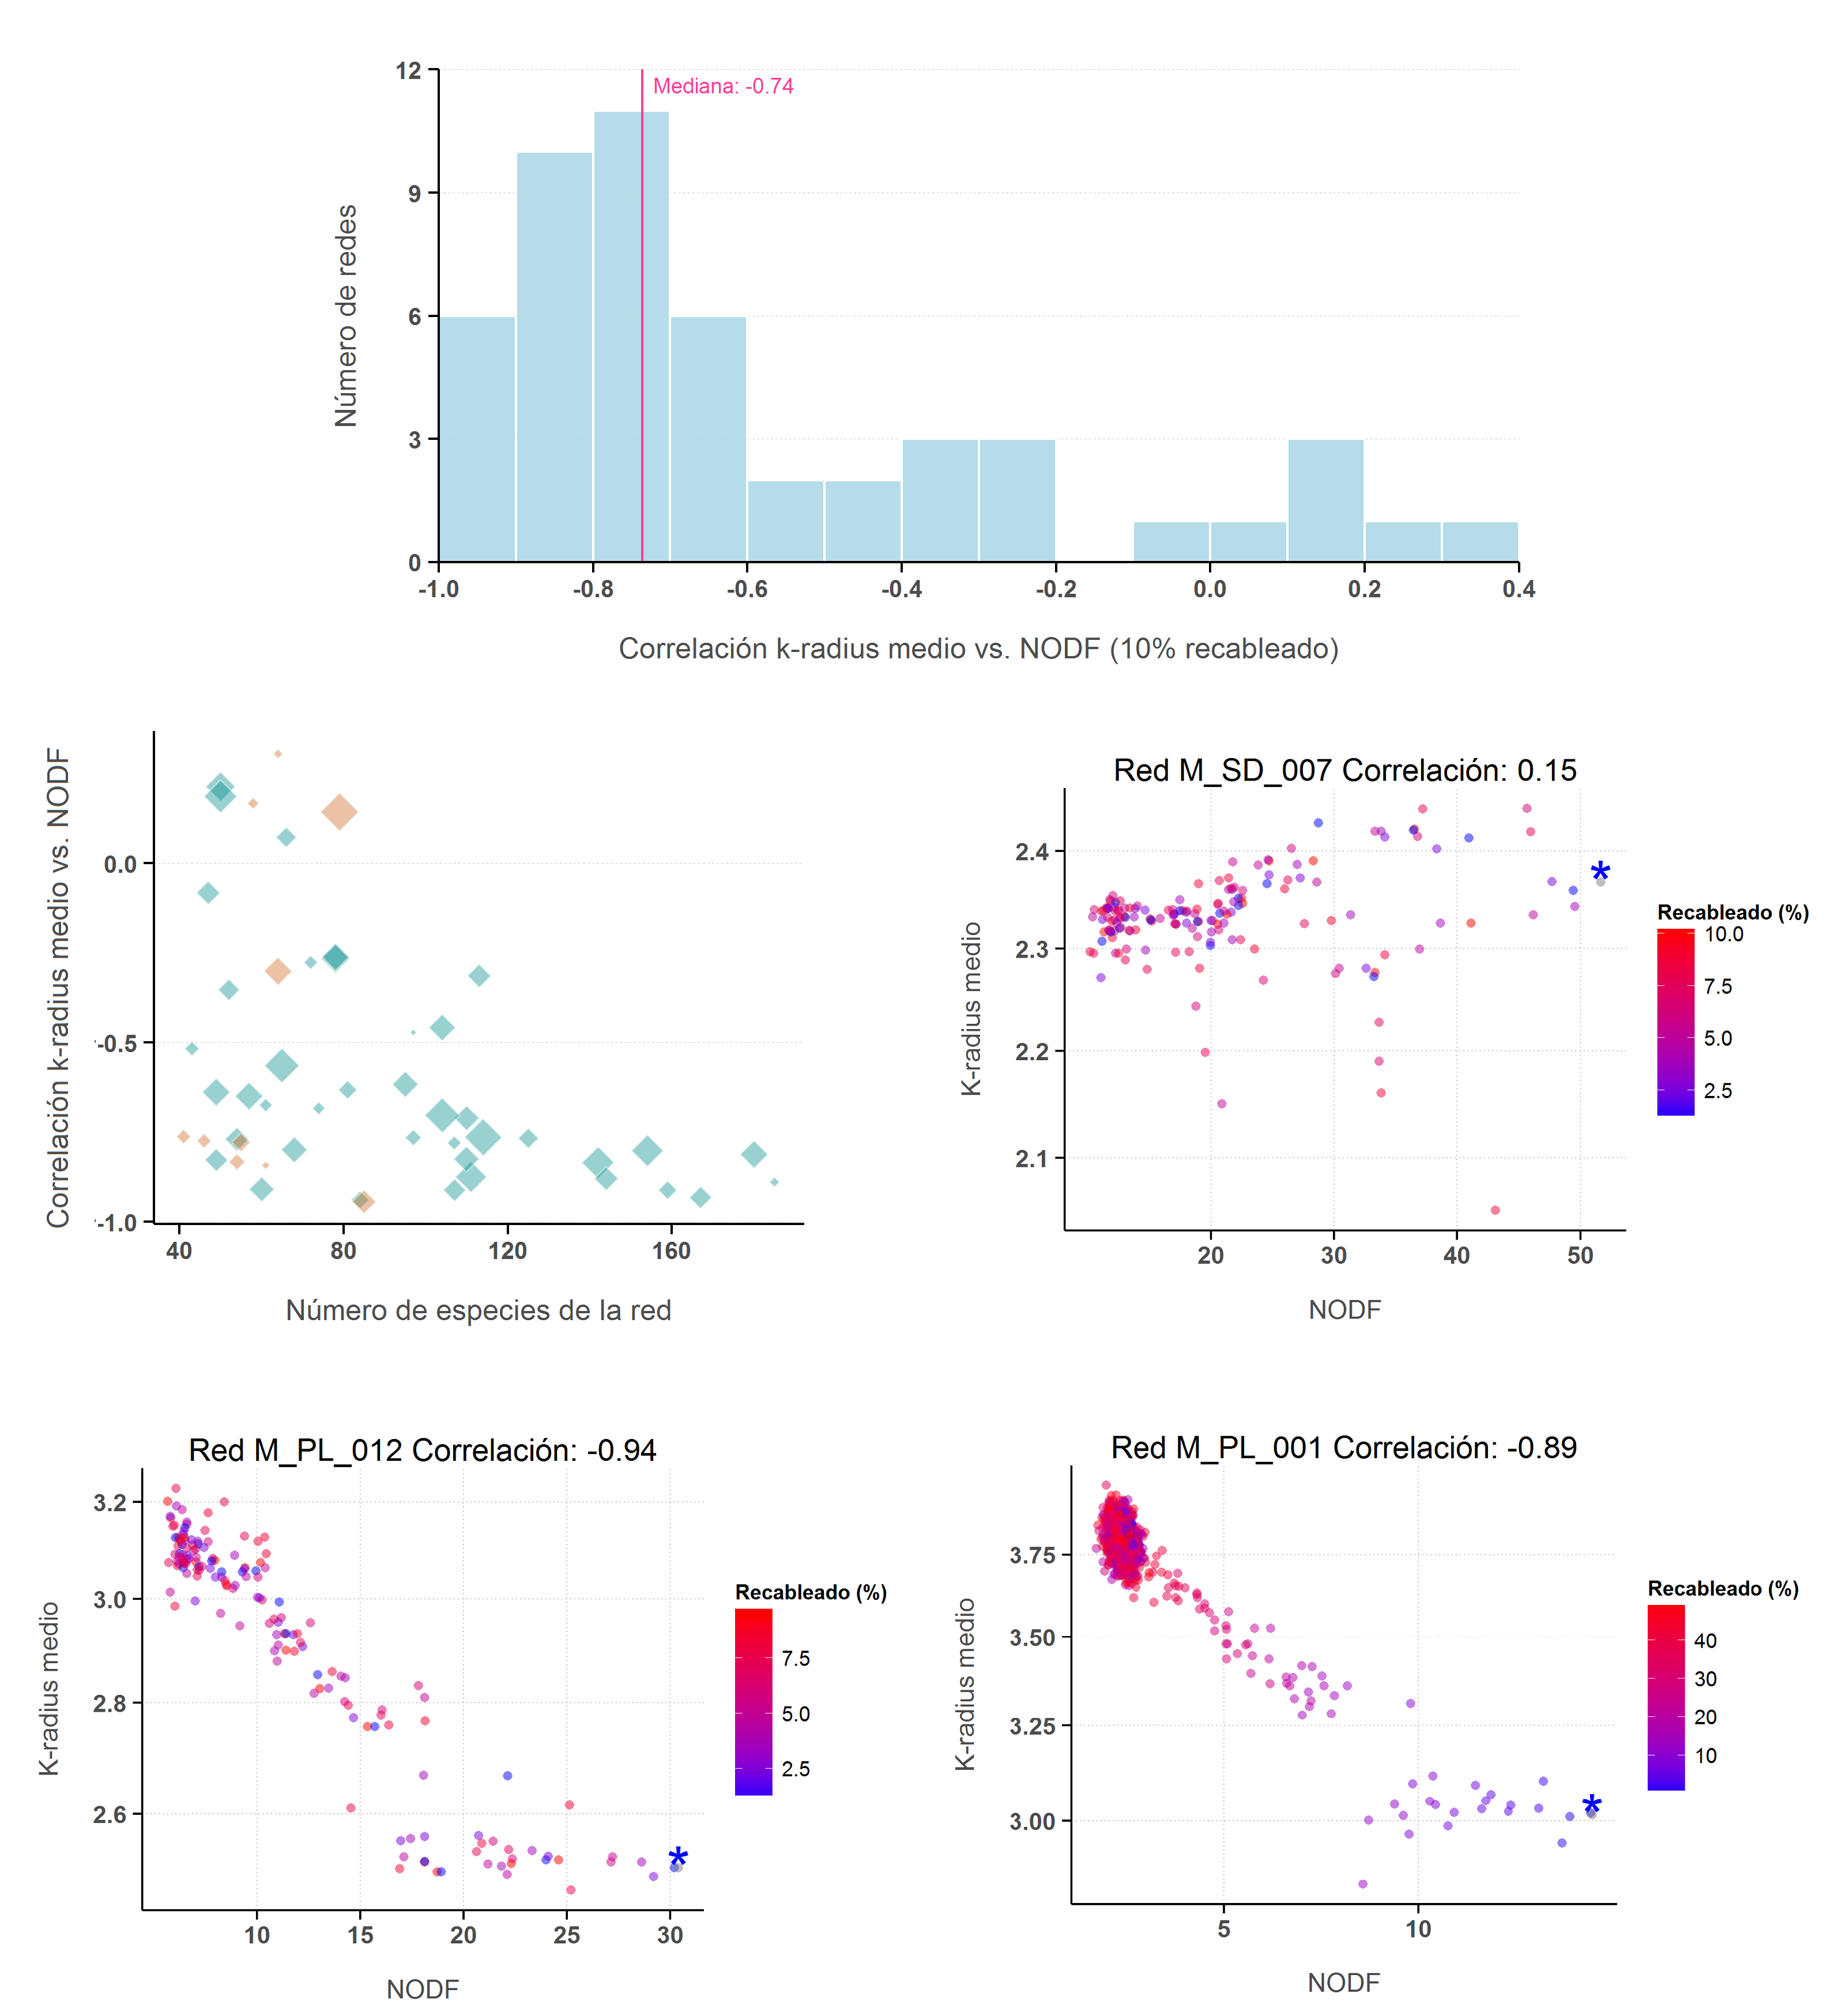
\includegraphics[scale=0.58]{ESTATICA_histo_corr_rewiring.png}
\caption {Resultados del experimento de recableado. Histograma de correlación $\overline {k}_{radius}$ y $NODF$, para un máximo del 10\% de enlaces; dispersión en función del tamaño de la red y gráficas para tres redes. En estas últimas el asterico azul indica el valor de la red original, sin modificar ninguna conexión.}
\label{fig:ESTATICA_histo_corr_rewiring}
\end{figure}

El histograma representa los valores de la correlación entre las dos magnitudes aludidas cuando en el experimento se recablean hasta un 10\% de los enlaces. Para la mayoría de las redes se obtienen correlaciones en torno al valor $-0,84$ que se encontró en el apartado anterior. Un pequeño porcentaje de reconexiones hace que $NODF$ se reduzca y que $\overline {k}_{radius}$ aumente de una manera predecible (véase la figura correspondiente a la red $M\_PL\_012$ en la fila inferior). Para las redes que se comportan así, un mayor porcentaje de reconexiones no supone un gran cambio en el estado final. la gráfica de la red $M\_PL\_010$ se ha obtenido cambiando hasta la mitad de los enlaces. Hay una zona de atracción en torno a $\overline {k}_{radius}$ de valor $0,35$ y $NODF$ casi nula, que representa una configuración aleatoria de la red muy alejada de la real.

Hay un porcentaje no despreciable de redes que no siguen esa variación para las que el experimento arroja valores reducidos de correlación e incluso positivos. Es el caso, por ejemplo, de $M\_SD\_007$. Un mínimo cambio destruye el anidamiento sin alterar de manera sustancial el $\overline {k}_{radius}$. Buscando el origen de este comportamiento dispar, se ha representado en la fila intermedia de la figura un diagrama de dispersión que relaciona el valor de la correlación con el número de especies de la red y con la asimetría. Esta se mide como el valor absoluto de la diferencia entre el número de especies de ambas clases dividida por su suma (tabla \ref{table:table_rewiring}) . El área correspondiente al rombo de cada especie es proporcional a esta cantidad. De la gráfica podemos deducir que cuanto mayor es el tamaño de la red, la correlación lineal entre $NODF$ y $log(\overline {k}_{radius})$ tiene mayor tendencia a mantenerse aunque cambie un pequeño porcentaje de conexiones. Para redes más pequeñas, el factor que destruye con mayor rapidez el anidamiento es la asimetría, y la red $M\_SD\_007$ es un caso extremo, con $72$ especies de plantas, solo $7$ de polinizadores y una estructura muy peculiar como se verá en el próximo capítulo de visualizaciones. Estas redes asimétricas son mucho más sensibles a las reconexiones, porque hay una mayor probabilidad de alterar la \textit{k-shell} máxima.

Lo que muestra cualitativamente este experimento, es que cuanto  mayores son el tamaño y la simetría, las redes parecen menos destructibles ante pequeños cambios. El valor de la correlación del experimento de recableado podría utilizarse como indicador numérico de la resistencia a una variación de las condiciones ambientales.

% Table generated by Excel2LaTeX from sheet 'Hoja1'
\begin{table}[ht!]
  \centering
  \tiny
    \begin{tabular}{lrrrr}
    \toprule
    $Red$ & $Plantas$ & $Animales$ & $Asimetría$ & $Correlación \overline r_{radius} y NODF$ \\
    \midrule
    M\_PL\_001 & 84   & 101  & 0,09 & -0,89 \\
    M\_PL\_002 & 43   & 64   & 0,20 & -0,78 \\
    M\_PL\_003 & 36   & 25   & 0,18 & -0,67 \\
    M\_PL\_004 & 12   & 102  & 0,79 & -0,76 \\
    M\_PL\_006 & 17   & 61   & 0,56 & -0,27 \\
    M\_PL\_007 & 16   & 36   & 0,38 & -0,35 \\
    M\_PL\_008 & 11   & 38   & 0,55 & -0,64 \\
    M\_PL\_009 & 24   & 118  & 0,66 & -0,83 \\
    M\_PL\_010 & 31   & 76   & 0,42 & -0,91 \\
    M\_PL\_012 & 29   & 55   & 0,31 & -0,94 \\
    M\_PL\_013 & 9    & 56   & 0,72 & -0,56 \\
    M\_PL\_014 & 29   & 81   & 0,47 & -0,71 \\
    M\_PL\_017 & 25   & 79   & 0,52 & -0,46 \\
    M\_PL\_018 & 39   & 105  & 0,46 & -0,88 \\
    M\_PL\_019 & 40   & 85   & 0,36 & -0,77 \\
    M\_PL\_020 & 20   & 91   & 0,64 & -0,87 \\
    M\_PL\_022 & 21   & 45   & 0,36 & 0,07 \\
    M\_PL\_023 & 23   & 72   & 0,52 & -0,62 \\
    M\_PL\_025 & 13   & 44   & 0,54 & -0,65 \\
    M\_PL\_026 & 105  & 54   & 0,32 & -0,91 \\
    M\_PL\_027 & 18   & 60   & 0,54 & -0,26 \\
    M\_PL\_028 & 41   & 139  & 0,54 & -0,81 \\
    M\_PL\_029 & 49   & 118  & 0,41 & -0,93 \\
    M\_PL\_030 & 28   & 53   & 0,31 & -0,63 \\
    M\_PL\_031 & 48   & 49   & 0,01 & -0,47 \\
    M\_PL\_033 & 13   & 34   & 0,45 & -0,08 \\
    M\_PL\_034 & 26   & 128  & 0,66 & -0,80 \\
    M\_PL\_035 & 61   & 36   & 0,26 & -0,76 \\
    M\_PL\_037 & 10   & 40   & 0,60 & 0,21 \\
    M\_PL\_038 & 8    & 42   & 0,68 & 0,19 \\
    M\_PL\_039 & 17   & 51   & 0,50 & -0,80 \\
    M\_PL\_040 & 29   & 43   & 0,19 & -0,28 \\
    M\_PL\_041 & 31   & 43   & 0,16 & -0,68 \\
    M\_PL\_043 & 28   & 82   & 0,49 & -0,82 \\
    M\_PL\_045 & 17   & 26   & 0,21 & -0,52 \\
    M\_PL\_046 & 16   & 44   & 0,47 & -0,91 \\
    M\_PL\_050 & 14   & 35   & 0,43 & -0,83 \\
    M\_PL\_051 & 14   & 90   & 0,73 & -0,70 \\
    M\_PL\_052 & 15   & 39   & 0,44 & -0,77 \\
    M\_PL\_058 & 32   & 81   & 0,43 & -0,31 \\
    M\_SD\_003 & 25   & 16   & 0,22 & -0,76 \\
    M\_SD\_004 & 34   & 20   & 0,26 & -0,83 \\
    M\_SD\_007 & 72   & 7    & 0,82 & 0,14 \\
    M\_SD\_010 & 50   & 14   & 0,56 & -0,30 \\
    M\_SD\_012 & 35   & 29   & 0,09 & 0,30 \\
    M\_SD\_013 & 36   & 19   & 0,31 & -0,78 \\
    M\_SD\_016 & 24   & 61   & 0,44 & -0,94 \\
    M\_SD\_018 & 29   & 32   & 0,05 & -0,84 \\
    M\_SD\_020 & 25   & 33   & 0,14 & 0,17 \\
    M\_SD\_021 & 18   & 28   & 0,22 & -0,77 \\
    \bottomrule
    \end{tabular}%
  \caption{\label{table:table_rewiring} Resultados del experimento de recableado de hasta un 10\% de enlaces.}
\end{table}%


\subsection{Rendimiento del algoritmo de destrucción}

Como hemos indicado, los resultados de nuestro algoritmo de destrucción se comparan con los obtenidos con \textit{MusRank}, un procedimiento de alto rendimiento. Tras probar diversas posibles combinaciones de los \textit{k-parámetros} encontramos que la más eficiente se basa en ordenar las especies primero por su \textit{k-shell}, a igualdad de  \textit{k-shell} por su $k_{radius}$, y a igualdad de ambos parámetros, por su $k_{degree}$. El área bajo la curva de extinción se utiliza para medir la velocidad de destrucción (mayor cuanto más pequeña). Por ejemplo, la figura \ref{fig:ESTATICA_destruction_comparativa_dosredes} muestra el tamaño de la componente gigante superviviente en función de la fracción de extinciones primarias para la red de polinizadores $M\_PL\_010$ (Elberling \& Olesen, no publicada). A la izquierda, el proceso de destrucción siguiendo el {MusRank}, a la derecha, según la ordenación basada en \textit{k-shell}. Mientras que con \textit{MusRank} la pendiente decreciente permanece casi constante, con \textit{k-shell} puede verse como al eliminarse la \textit{k-shell} máxima se produce una caída abrupta en el número de especies supervivientes.

\begin{figure}[h!]
\centering
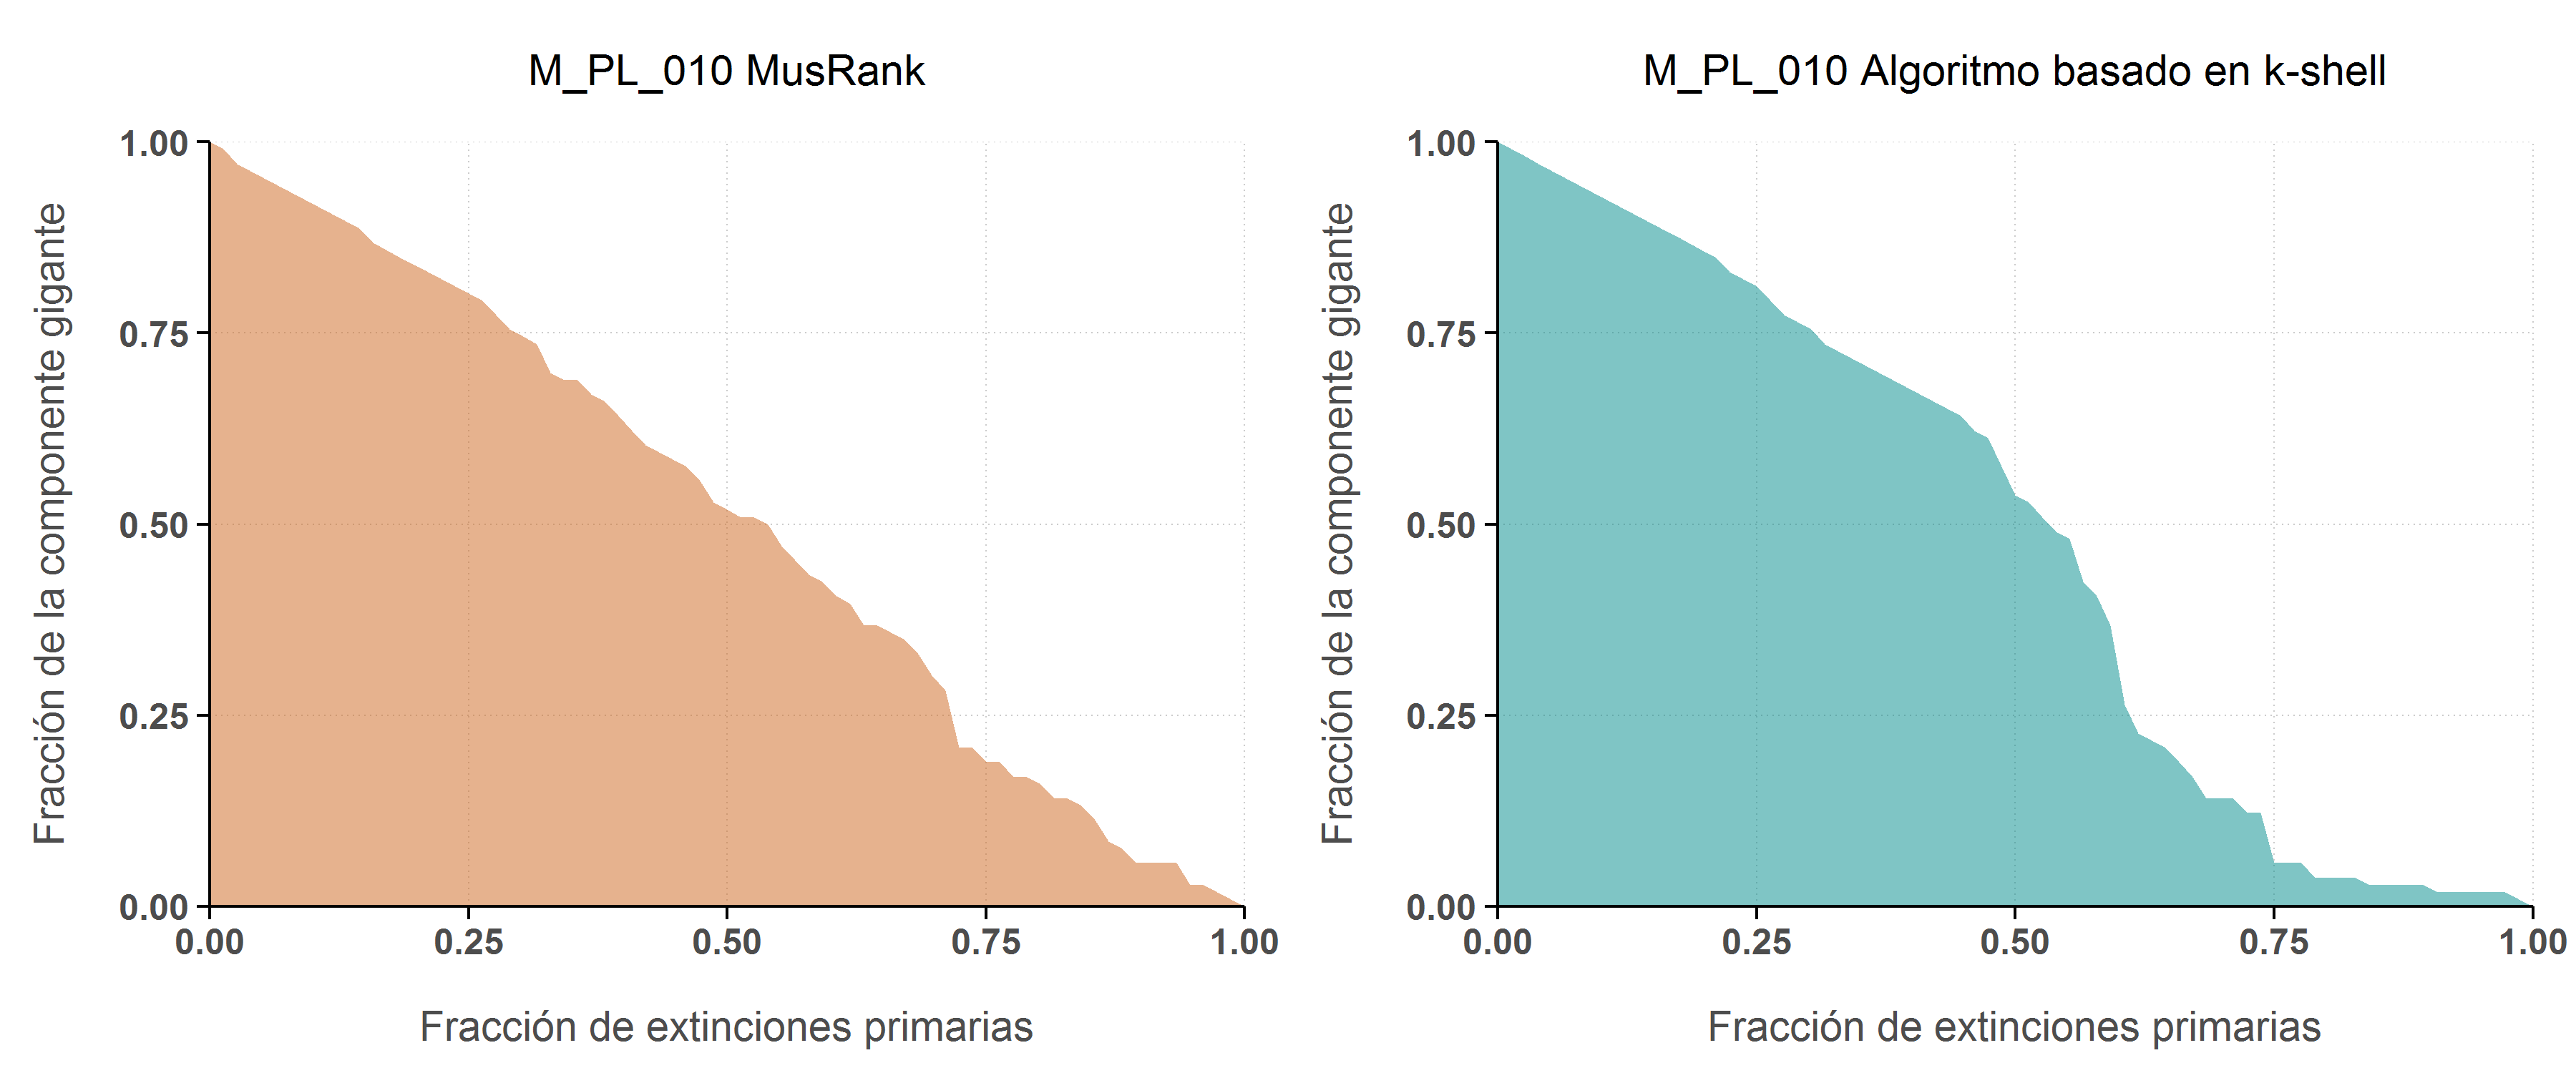
\includegraphics[scale=0.45]{ESTATICA_destruction_comparativa_dosredes.png}
\caption {Curva de extinción de la red planta-polinizador $M\_PL\_010$ para ambos algoritmos}
\label{fig:ESTATICA_destruction_comparativa_dosredes}
\end{figure}

La figura \ref{fig:ESTATICA_destructions_comparison} muestra la comparativa de rendimiento para las $89$ redes del estudio, medida como la diferencia de áreas normalizadas según \textit{MusRank} y según \textit{k-shell}. Si es positiva, el segundo procedimiento es más destructivo y por tanto más eficaz, y viceversa (última columna de la tabla \ref{table:table_results}). la destrucción basada en \textit{k-shell} es más rápida para $57$ de las $59$ redes del tipo \textit{planta-polinizador}. 

\begin{figure}[h!]
\centering
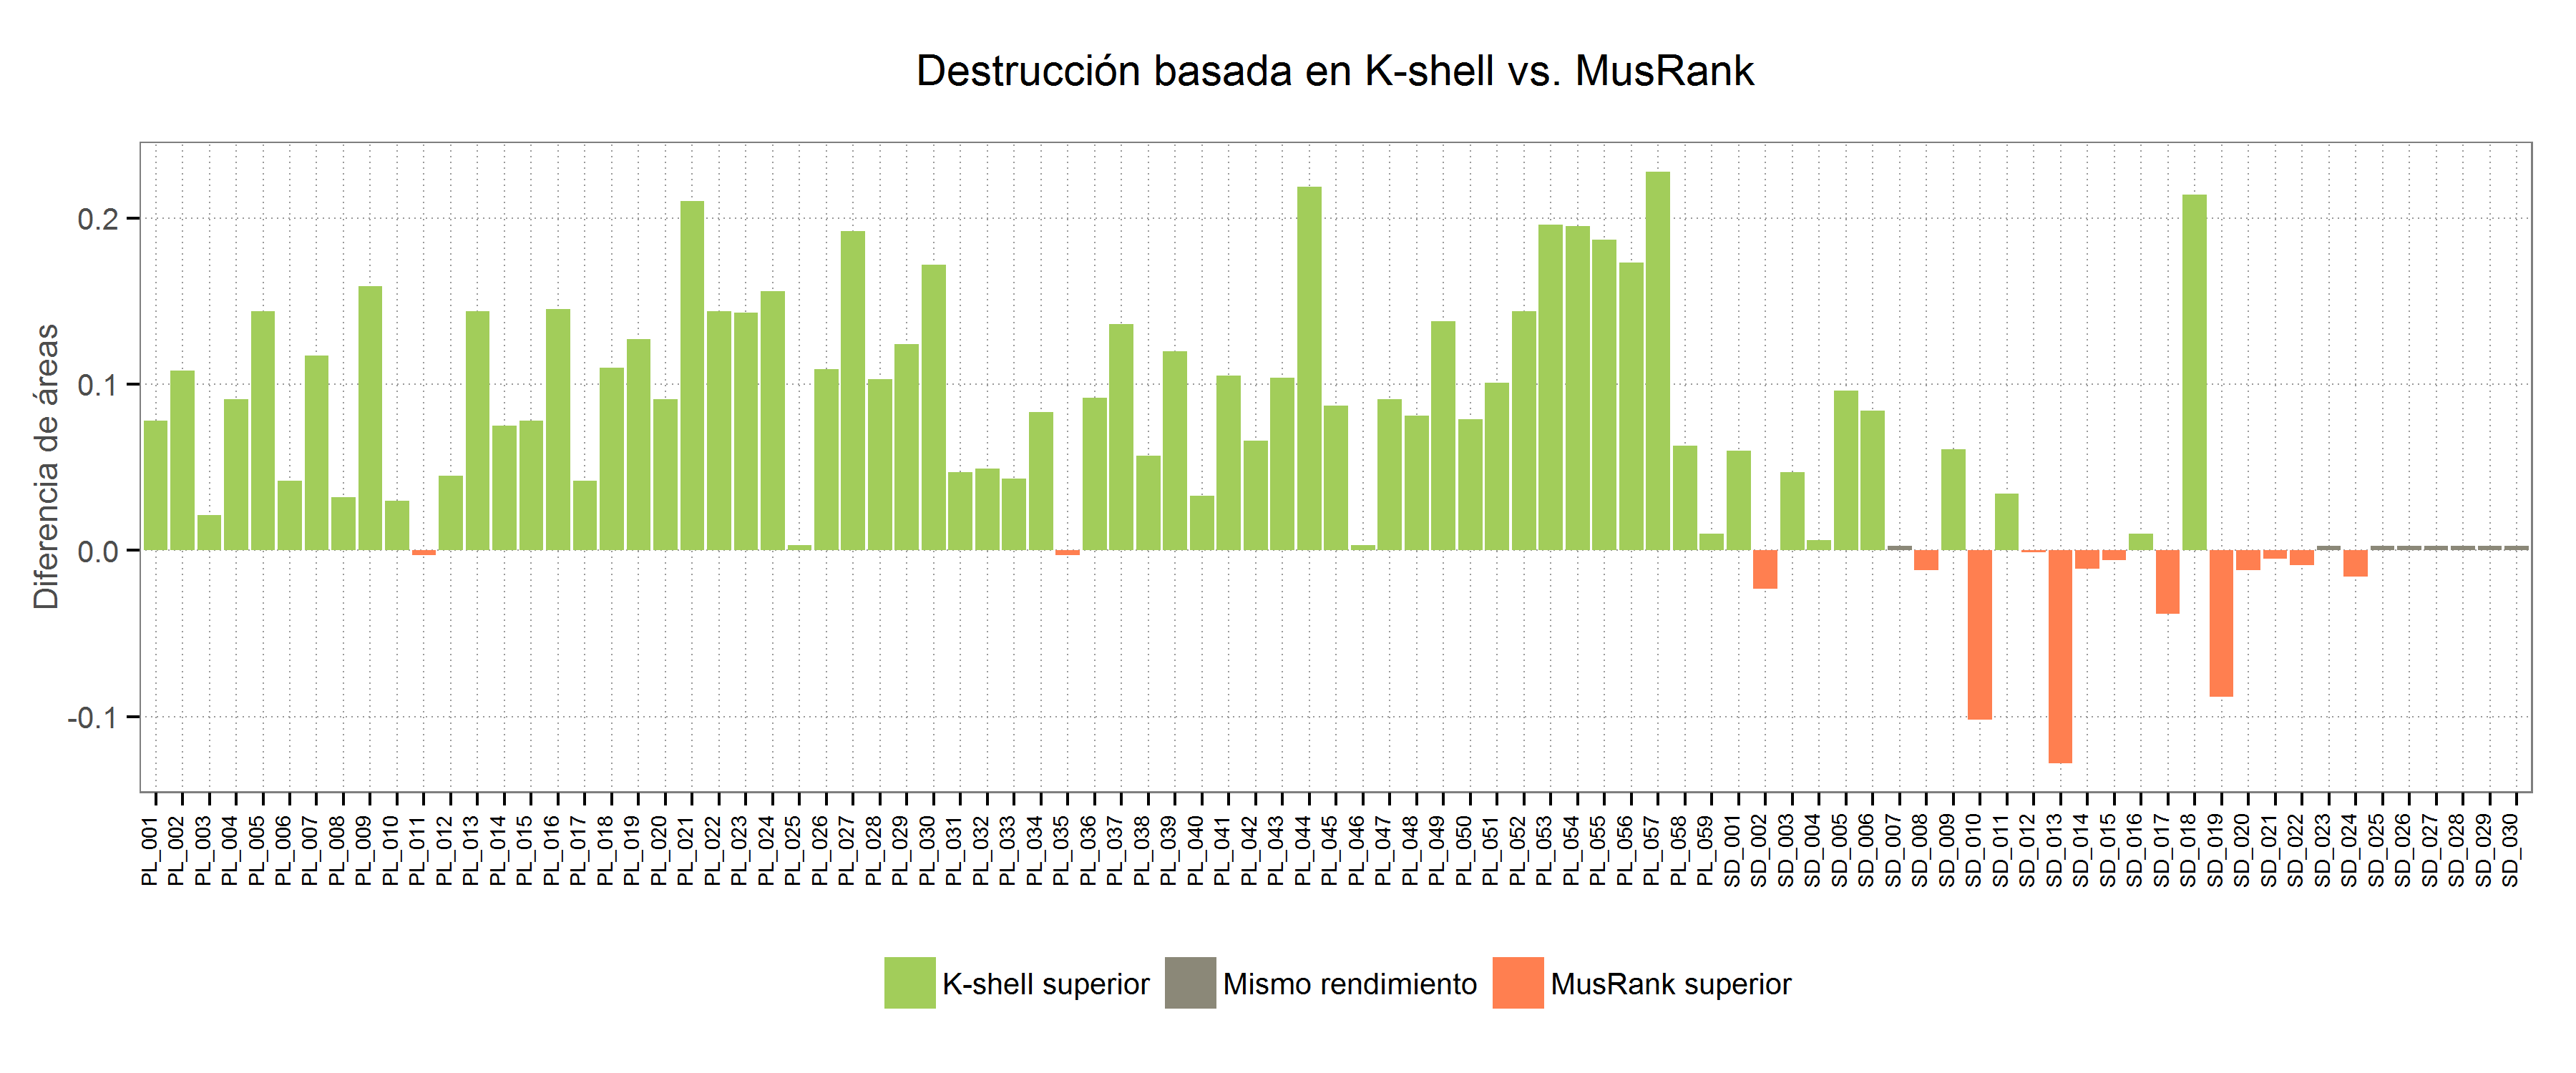
\includegraphics[scale=0.5]{ESTATICA_destructions_comparison.png}
\caption {Comparison of destruction performance of \textit{k-shell} ranking based algorithm vs. \textit{MusRank}}
\label{fig:ESTATICA_destructions_comparison}
\end{figure}

La diferencia de rendimiento no es tan llamativa para las de dispersores de semillas, \textit{MusRank} supera a \textit{k-shell} en $13$ casos, es más lento en $10$ y equivalente en $y$. Como hemos visto, las redes de este tipo en la colección estudiada son de menor tamaño y más anidades. El procedimiento basado en \textit{k-shell} parece ser mejor predictor de la resistencia de la red en comunidades grandes y modulares, mientras que \textit{MusRank} alcanza mejor rendimiento para redes pequeñas y fuertemente anidadas.

\section{Conclusiones}

La \textit{descomposición k-core} proporciona una sólida base para el análisis del mutualismo. Hemos demostrado como las \textit{k-magnitudes} definidas como propiedades surgidas del procedimiento, permiten conocer en detalle la estructura de las redes. En particular, al promediar los valores locales para todo el sistema, $\overline {k}_{radius}$ y $\overline {k}_{degree}$ muestran una fuerte correlación con los observables globales $NODF$ y $Modularity$. 

Esta técnica descubre detalles internos de una forma natural, agrupando las especies en conjuntos que comparten propiedades topológicas. La identificación de las distintas \textit{k-shells} permite realizar estudios de estabilidad y resistencia. La simulación de perturbaciones externas puede concentrarse en la destrucción de las \textit{k-shells} más internas y observar el efecto para la supervivencia de la comunidad. 

La descomposición es también el criterio de una nueva ordenación de las especies. Hemos provocado extinciones primarias y evaluado la evolución del tamaño de la componente gigante. Los resultados muestra que el procedimiento de extinción basado en \textit{k-shell} obtiene un mejor renidmiento que \textit{MusRank} para casi todas las redes de polinizadores de la colección investigada, y es ligeramente peor para las de dispersores de semillas. La ordenación por \textit{k-core} es un buen predictor de la resistencia de red.

Aunque hemos enfocado el estudio en redes mutualistas, la técnica se puede extender a otros tipos de redes bipartitas, por ejemplo comensalistas. Relaciones bipartitas y con fuerte anidamiento, como las que aparecen en redes de innovación y comercio, podrían también beneficiarse de este análisis.
% Chapter Template

\chapter{Visualizaciones} % Main chapter title
\label{chapterVISUALIZACIONES}

Las visualizaciones son una herramienta imprescindible para el análisis de la información, y en particular en la ciencia de redes. La representación gráfica es básica en el análisis exploratorio pero también necesaria para la síntesis de resultados. Al trabajar con redes ecológicas se emplean gráficos de uso común en el análisis de redes sociales \cite{freeman2012social}. No ha habido apenas desarrollo de herramientas y gráficas específicas para este campo de aplicación \cite{yoon20043d, kazanci2007econet, lane2014visualization}.

En el estudio del mutualismo se utilizan sobre todo dos tipos de gráfico: el diagrama bipartito y la matriz de adyacencia. Ambos son sencillas y ponen de manifiesto la separación entre las clases de especies, pero tienen limitaciones importantes. En este capítulo proponemos dos tipos de visualización que se construyen utilizando las \textit{k magnitudes}

\label{VISUALIZACIÓN} % Change X to a consecutive number; for referencing this chapter elsewhere, use \ref{ChapterX}

%----------------------------------------------------------------------------------------
%	SECTION 1
%----------------------------------------------------------------------------------------

\section{Representaciones clásicas del mutualismo}

Las redes mutualistas son bipartitas y por ello no es de extraño que el diagrama bipartito haya sido el más empleado en la literatura. En este 
gráfico los nodos se disponen en dos filas paralelas, ya sean horizontales o verticales, y se unen aquellos que comparten enlace. Cuando el tamaño
de la red es reducido, este diagrama tan simple funciona de manera satisfactoria.

\begin{figure}[h!]
\centering
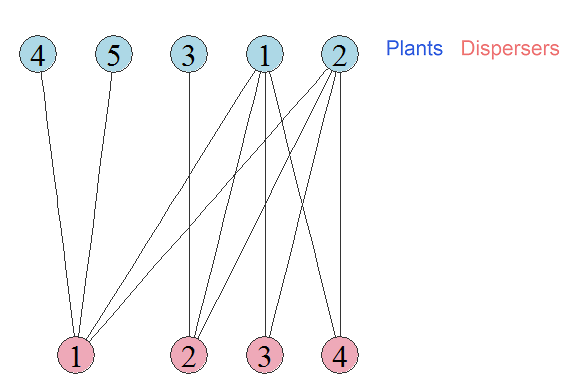
\includegraphics[scale=0.33]{Figures/VIS_SD_030_bipartita.png}
\caption{Diagrama bipartito de la red de dispersores de semillas que se usó como ejemplo de cálculo de las \textit{k magnitudes}. Véase la figura \ref{fig:ESTATICA_red_example}.}
\label{fig:Figures/VIS_SD_030_bipartita}
\end{figure}

En el ejemplo de la figura \ref{fig:Figures/VIS_SD_030_bipartita} puede distinguirse el núcleo de especies más conectadas (especies de plantas $1$ y $2$ y todos los polinizadores) y como las especialistas se conectan a él. Los enlaces se ven con claridad. No obstante, es difícil captar la estructura interna de la red como en la representación que utilizamos en la figura \ref{fig:ESTATICA_red_example}. El diagrama bipartito es ideal para redes de afiliación, en las que el dato clave es la conexión entre los nodos de ambas clases, pero no permite apreciar las interacciones indirectas entre elementos de una misma clase que comparten enlace con un nodo de la contraria.

\begin{figure}[h!]
\centering
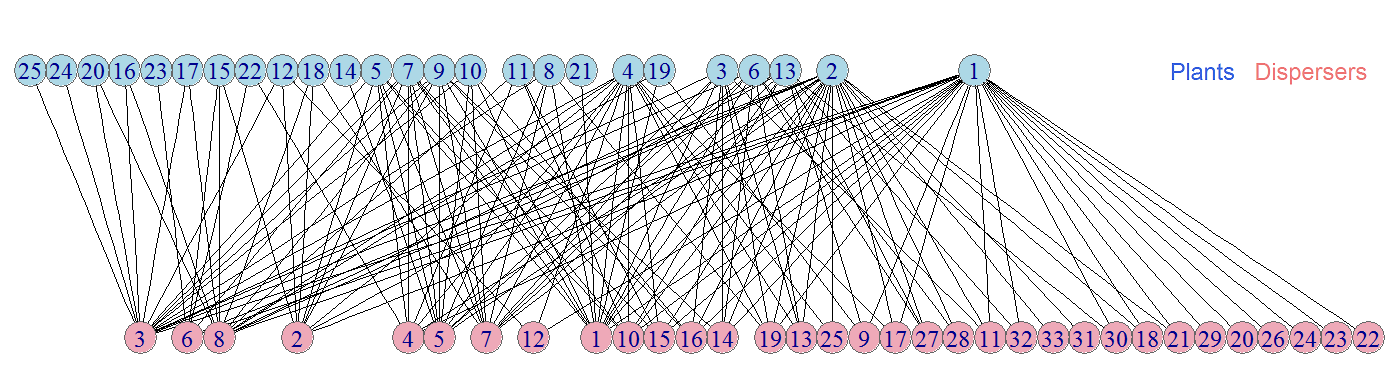
\includegraphics[scale=0.4]{Figures/VIS_bipartito_SD_020.png}
\caption{Red de dispersores en Nava Correhuelas, Sierra de Cazorla, España. Compilada por Pedro Jordano, no publicada.}
\label{fig:VIS_bipartito_SD_020}
\end{figure}

Cuando el número de especies supera unas pocas decenas, el diagrama bipartito se vuelve confuso. La red de la figura \ref{fig:VIS_bipartito_SD_020} tiene $58$ especies y $150$ enlaces, frente a $9$ especies y $11$ enlaces de la anterior. Es una red de dimensiones moderadas, pero es muy complicado seguir los detalles del gráfico. A pesar de ello, algunos autores consiguen resultados excelentes con redes de dimensiones similares a las de este segundo ejemplo, jugando con formas, colores y tamaños \cite{dakos2014critical}. Cuando se llega al centenar de especies, la zona central degenera en una mancha en la que es imposible distinguir los enlaces. Por este motivo, en la literatura sobre mutualismo no aparecen diagramas bipartitos de redes grandes. 

La matriz de adyacencia ofrece una visión más rica si los nodos se ordenan de la forma adecuada. Colocando los más conectados en la parte superior izquierda, es fácil localizar el núcleo de especies generalistas. Para redes pequeñas, el resultado es muy satisfactorio.

\begin{figure}[h!]
\centering
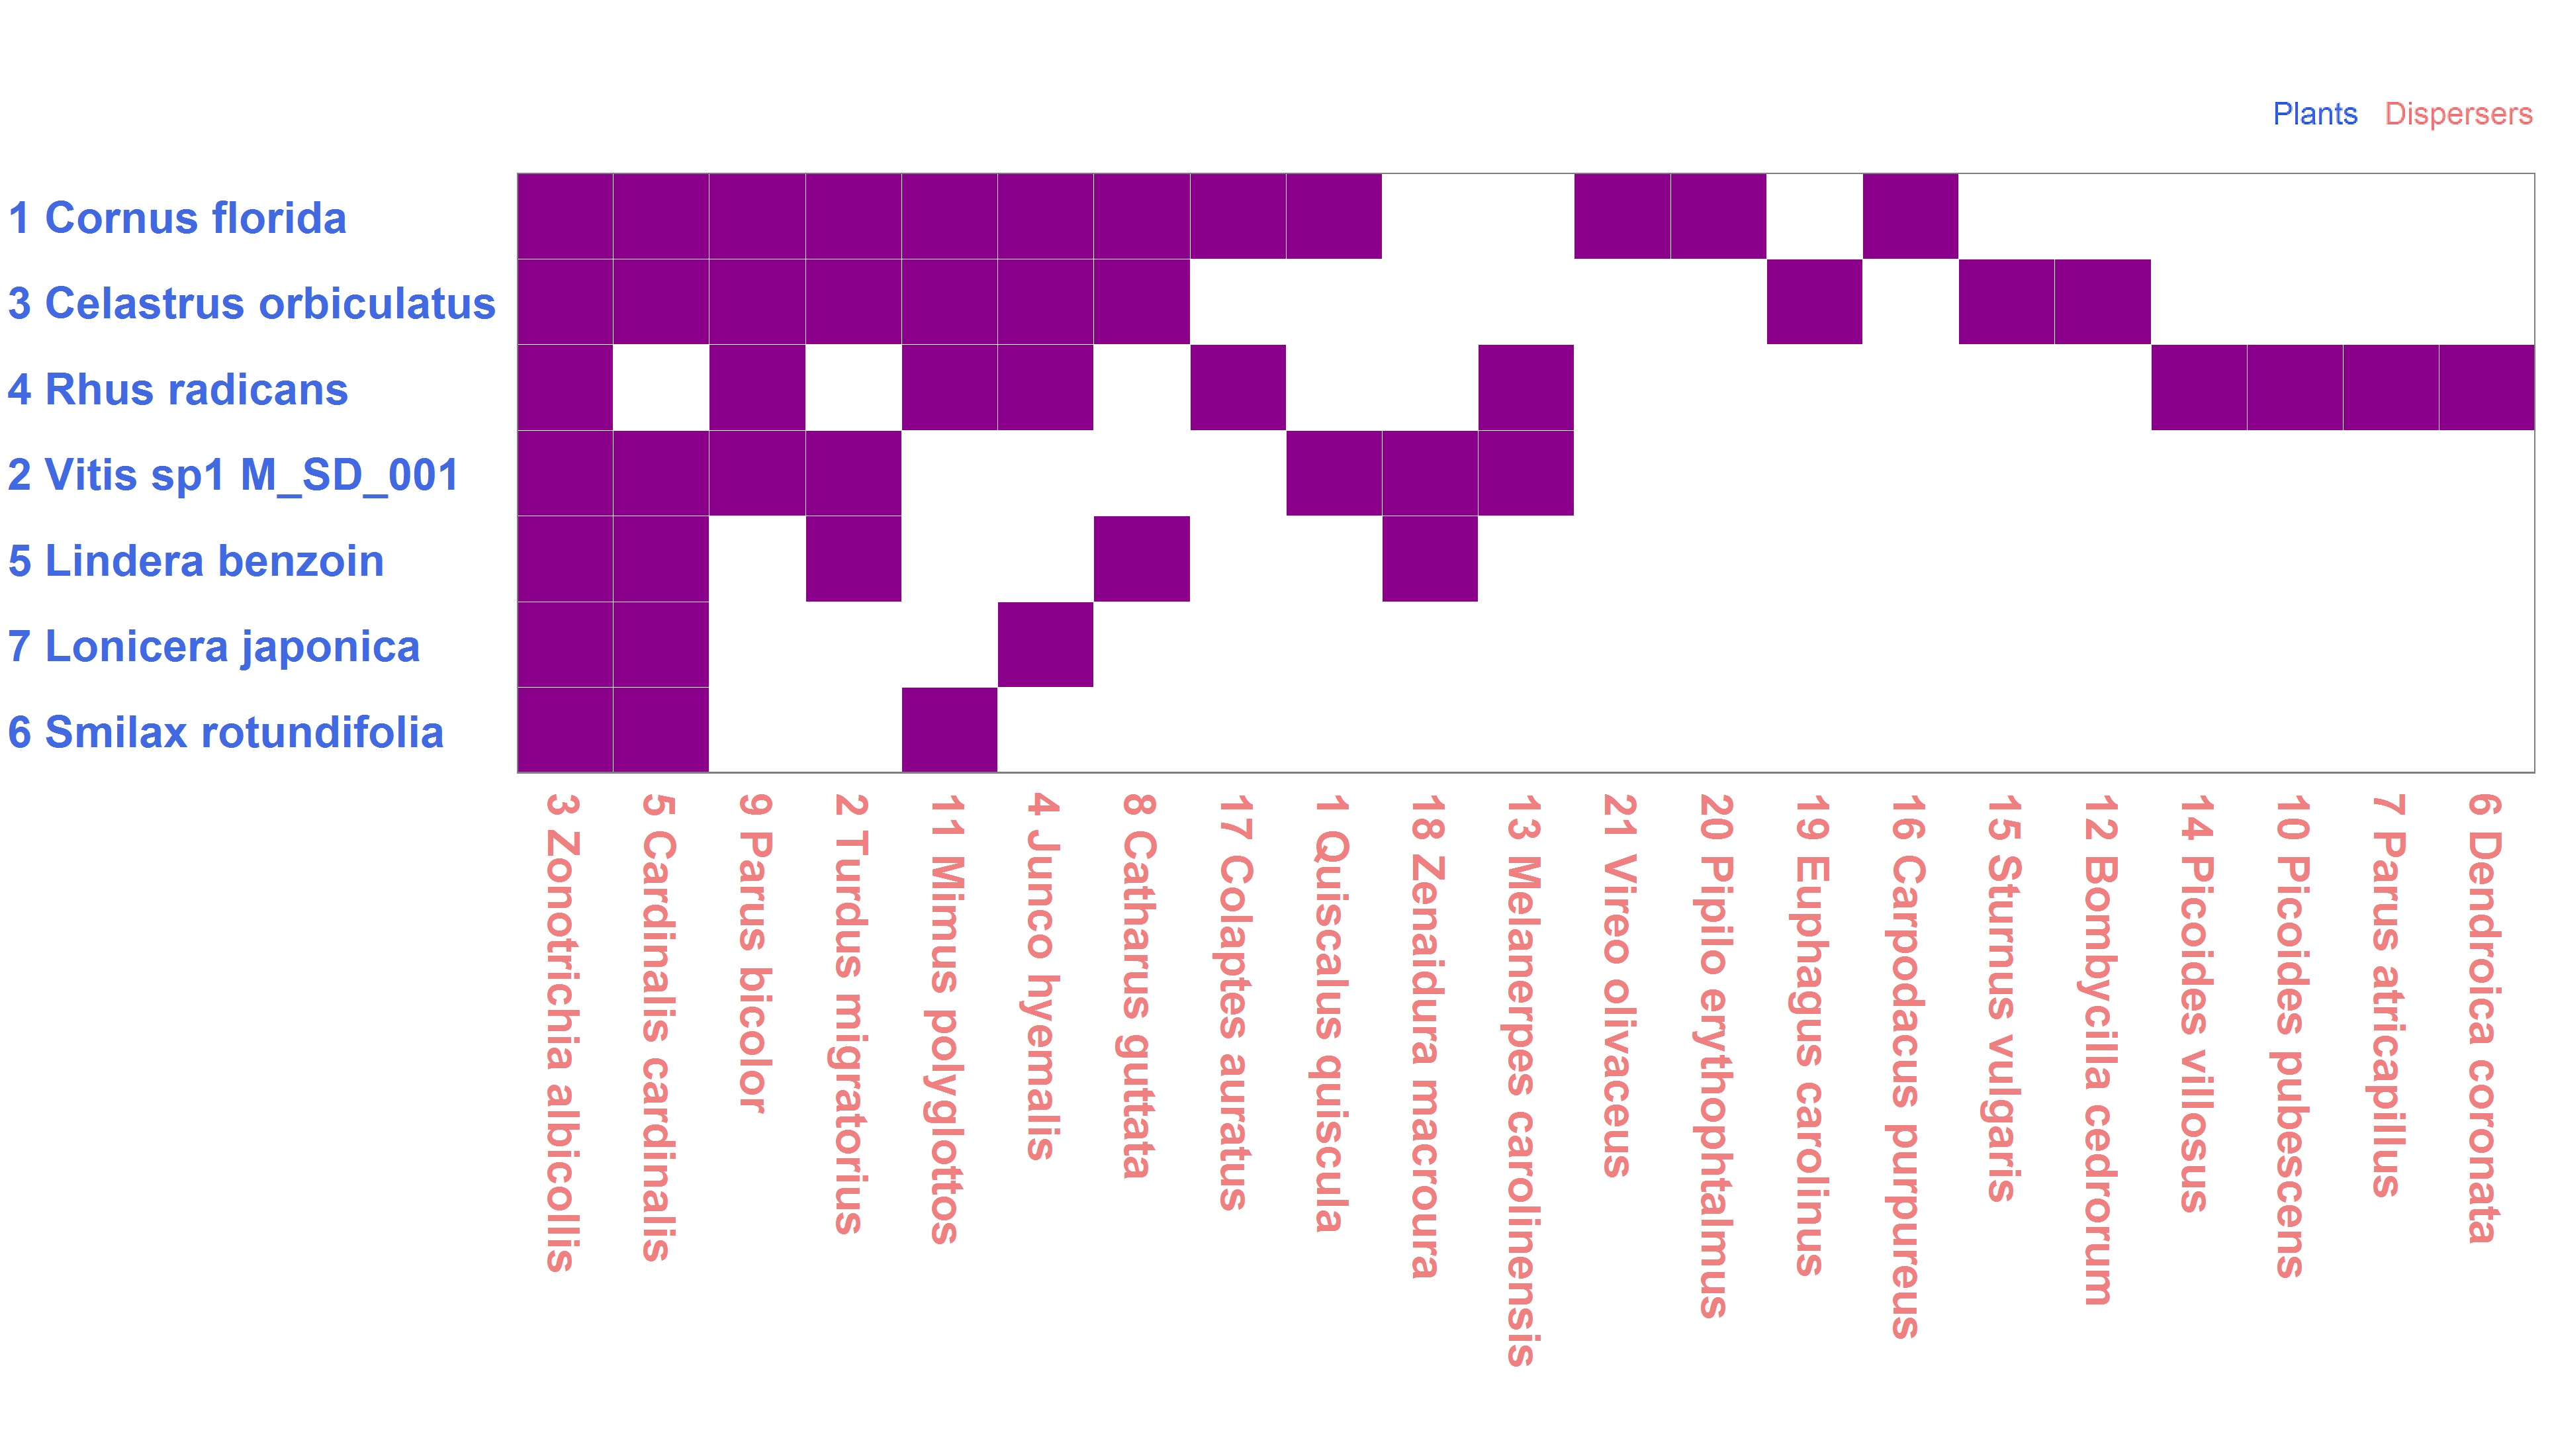
\includegraphics[scale=0.14]{Figures/VIS_matrix_SD_001.png}
\caption{Matriz de adyacencia de una red de dispersores en New Jersey \cite{baird1980selection}. Las casillas coloreadas indican la existencia de enlace.}
\label{fig:VIS_matrix_SD_001}
\end{figure}

Por el contrario, esta representación gráfica se vuelve también muy confusa para redes grandes, como muestra la figura \ref{fig:VIS_matrix_PL_001}.

\begin{figure}[hp!]
\centering
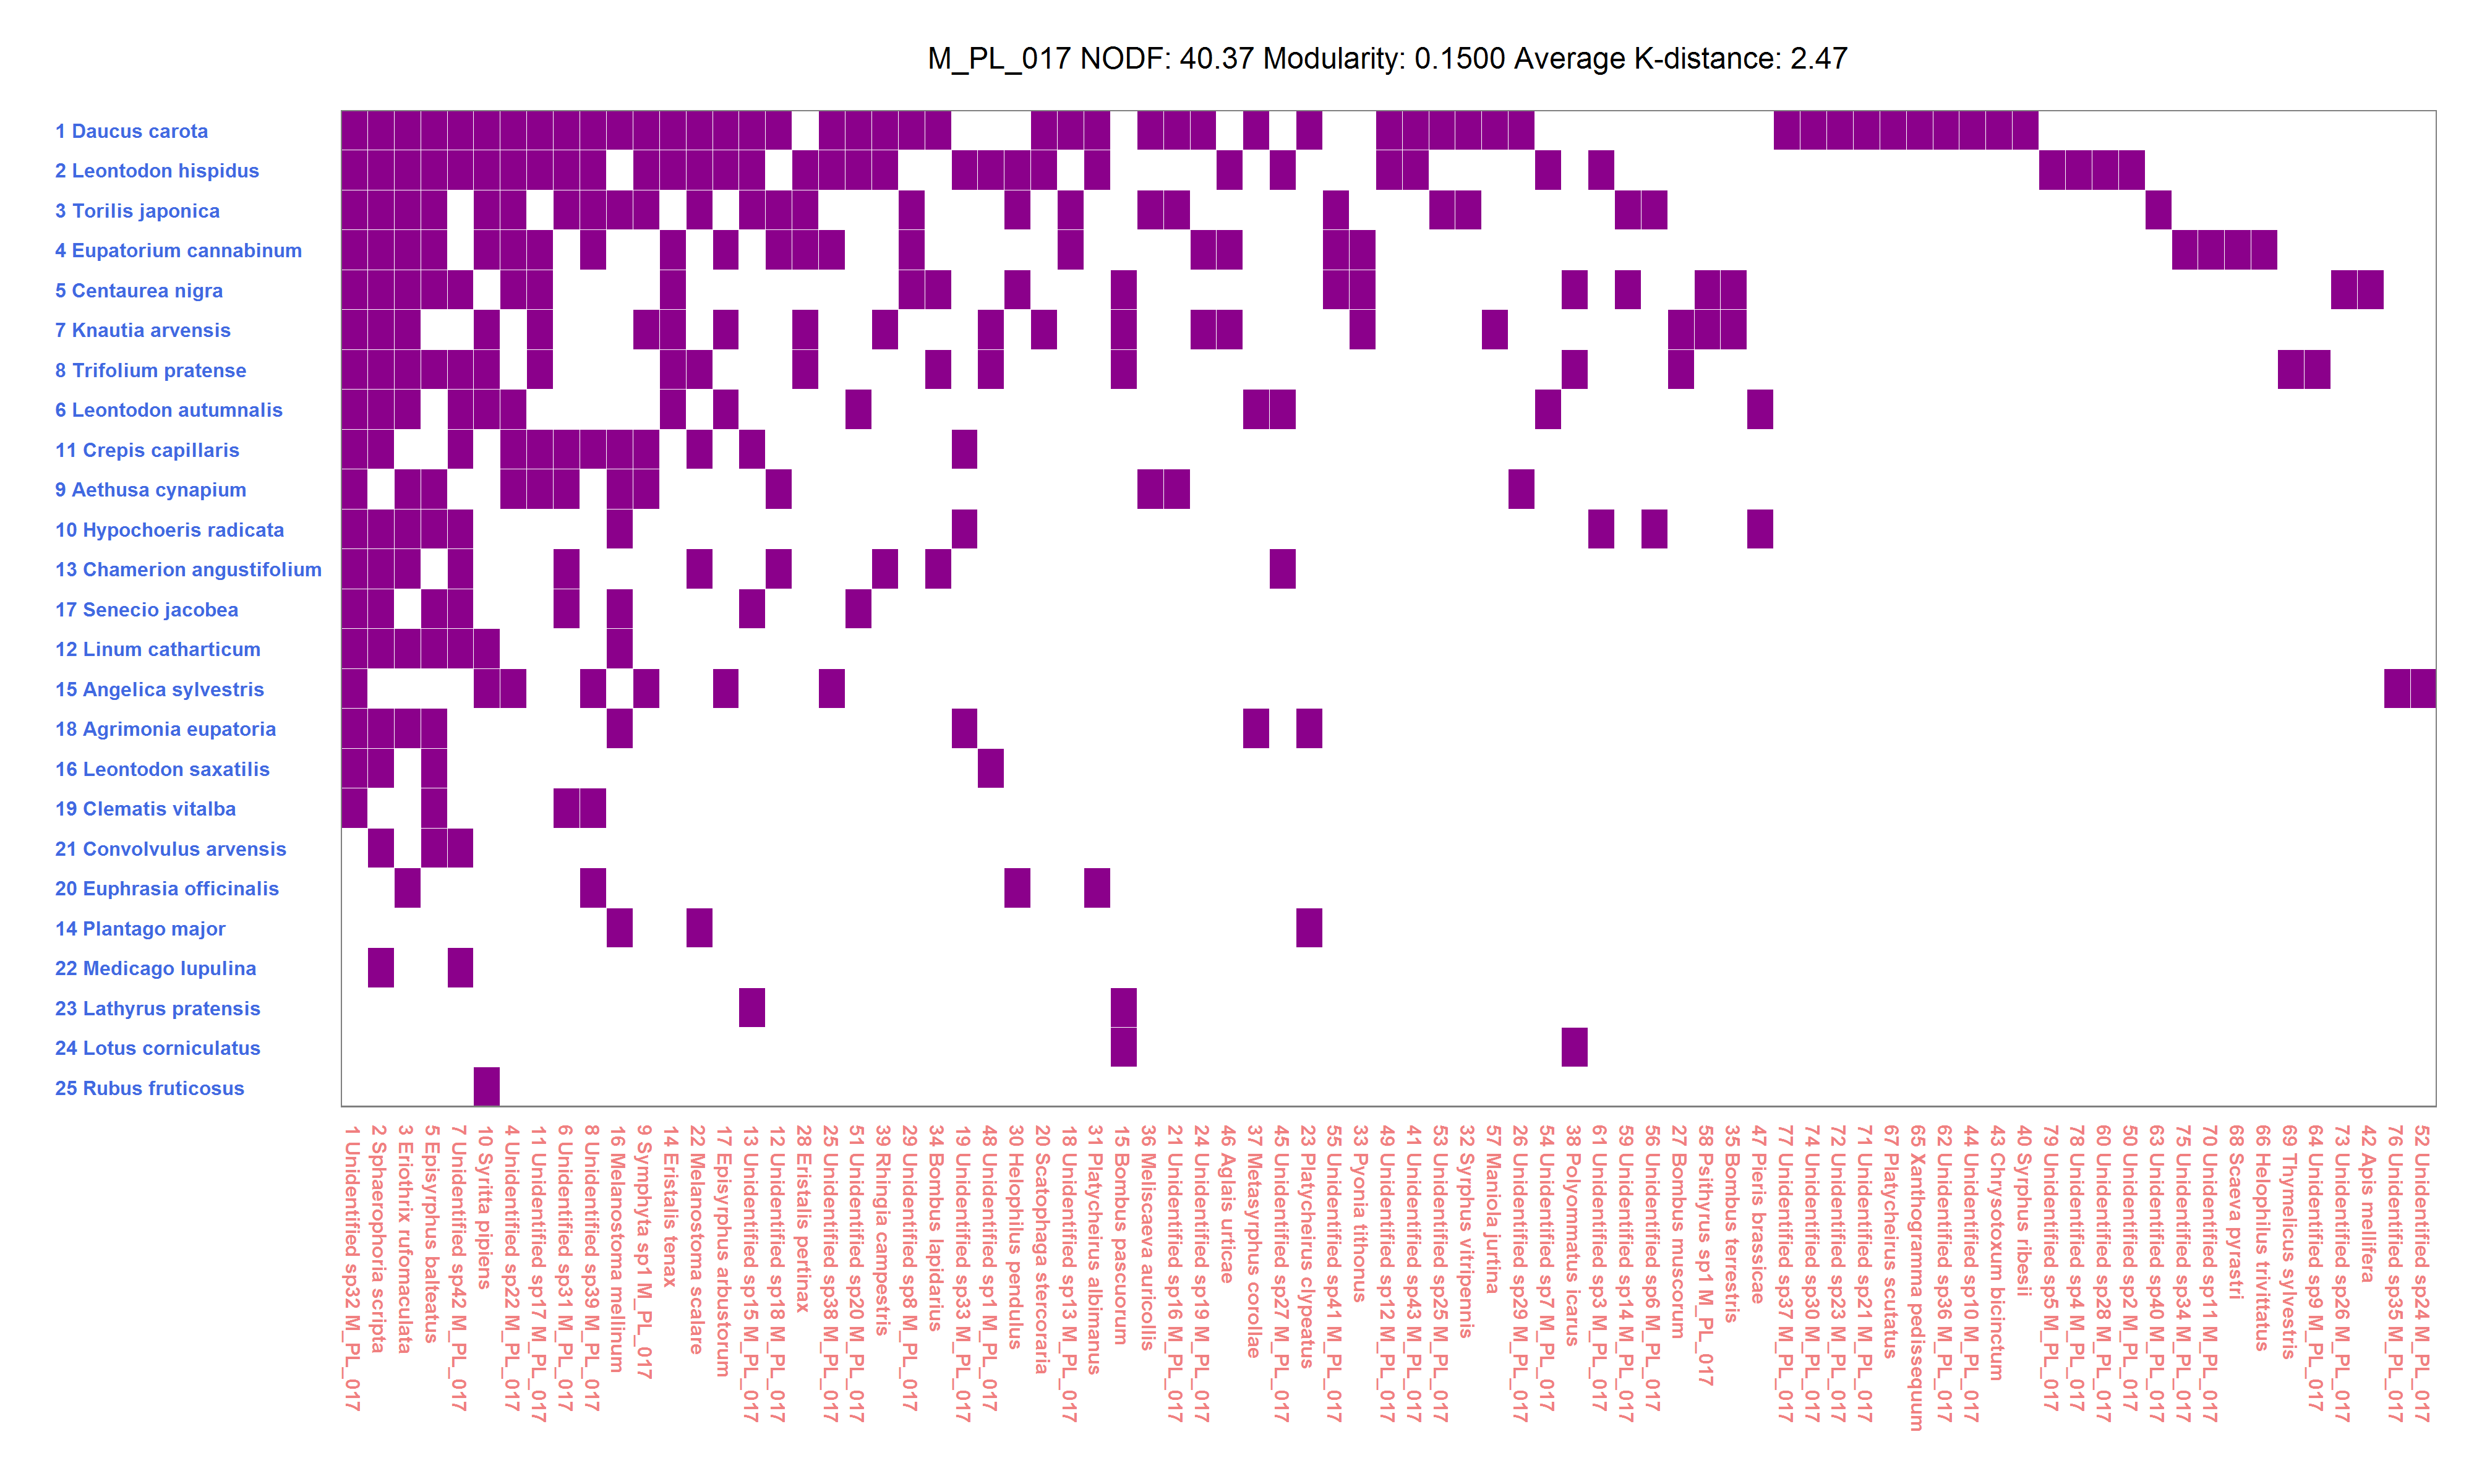
\includegraphics[scale=0.45]{Figures/VIS_M_PL_017_matrix.png}
\caption{Matriz de adyacencia de una red de polinizadores en Bristol, Inglaterra \cite{memmott1999structure}.}
\label{fig:VIS_matrix_PL_001}
\end{figure}

Una alternativa que algunos autores han explorado es utilizar representaciones convencionales para redes no bipartitas, asignando un color o forma específicos para cada clase \cite{mello2011missing,genini2010cheaters,toju2014assembly}. Esta solución tiene la ventaja de que se percibe mucho mejor la red y las relaciones indirectas que hemos mencionado. El precio que se paga es que los diagramas se vuelven muy complicados de entender con redes de tamaño medio (figura \ref{fig:VIS_grafos_weboflife}).

\begin{figure}[hp!]
\centering
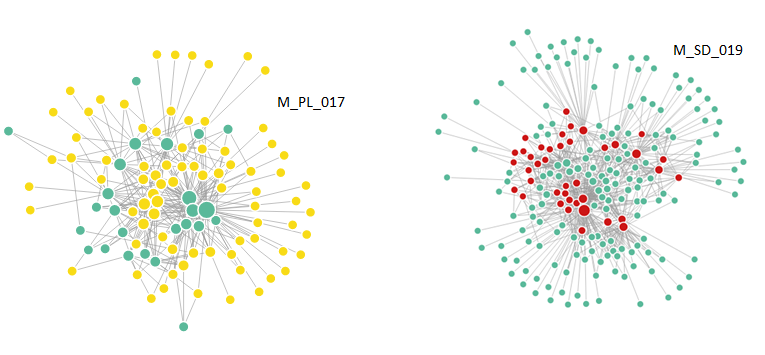
\includegraphics[scale=0.75]{Figures/VIS_grafos_weboflife.png}
\caption{Representación de dos redes de la colección \textit{web of  life} mediante la herramienta de visualización que ofrece la página web.}
\label{fig:VIS_grafos_weboflife}
\end{figure}

Estas limitaciones nos han llevado a diseñar visualizaciones específicamente adaptadas a las características de las redes mutualistas: bipartitas, con una fuerte jerarquía y en el rango de centenares de enlaces. 

\clearpage
\section{Visualizaciones basadas en \textit{k-magnitudes}}

En esta sección se describen dos nuevos tipos de visualización que se basan en las \textit{k magnitudes} definidas en el capítulo anterior: el diagrama polar y el diagrama zigurat.

\subsection{El diagrama polar}

El diagrama polar se inspira en el \textit{fingerprint plot}, desarrollado por Álvarez-Hamelin \textit{et al} y que se basa en la descomposición \textit{k-core} \cite{alvarez2005k}. Los autores emplearon esta técnica para reducir la información y poder visualizar redes muy grandes con índice $k$ máximo del orden de varias decenas. Los nodos se ubican de manera concéntrica, a una distancia que depende de su \textit{k-shell} y de las de sus vecinos. El tamaño de los nodos es proporcional al logaritmo del grado y el color indica la \textit{shell} a la que pertenecen. No se dibujan todos los enlaces, solo un pequeño porcentaje elegido al azar.

\begin{figure}[h!]
\centering
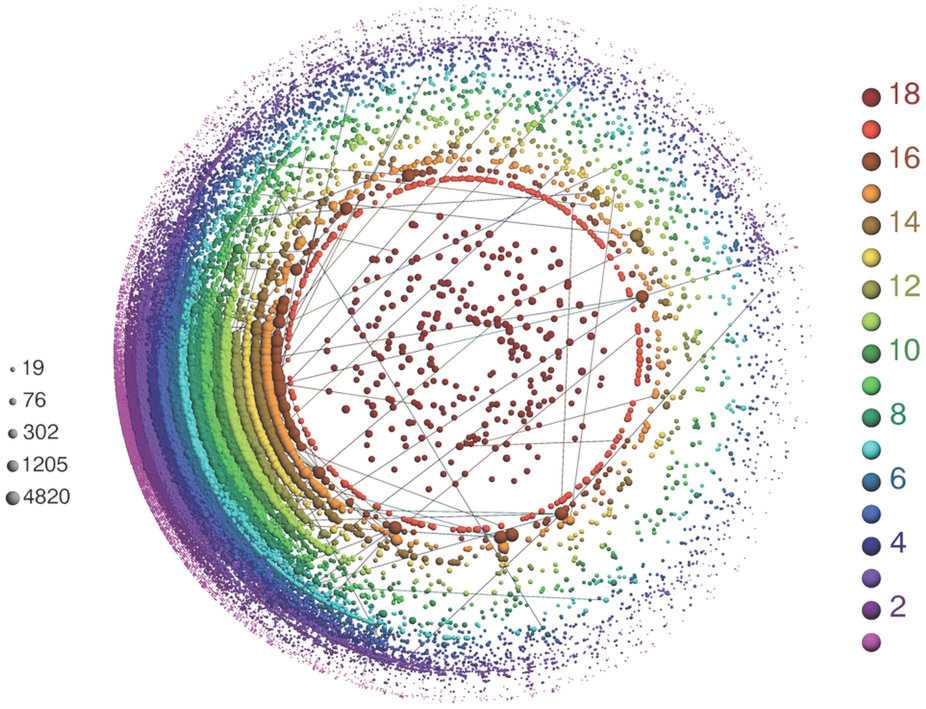
\includegraphics[scale=0.5]{Figures/VIS_fingerprint_plot.png}
\caption{\textit{Fingerprint plot} de la difusión de la noticia del descubrimiento del bosón de Higgs en Twitter \cite{de2013anatomy}. La imagen se generó con el software \texttt{LaNet-vi}, desarrollado por el equipo que creó este tipo de diagrama \cite{alvarez2008low}.}
\label{fig:VIS_M_PL_034_polar}
\end{figure}

Una versión evolucionada de esta forma de representar redes grandes usando la descomposición \textit{k-core} utiliza las \textit{k-shell} en lugar de los nodos. Estas se dibujan como círculos que se disponen en espiral alrededor de la \textit{shell} máxima (figura \ref{fig:VIS_taksim}).

\begin{figure}[h!]
\centering
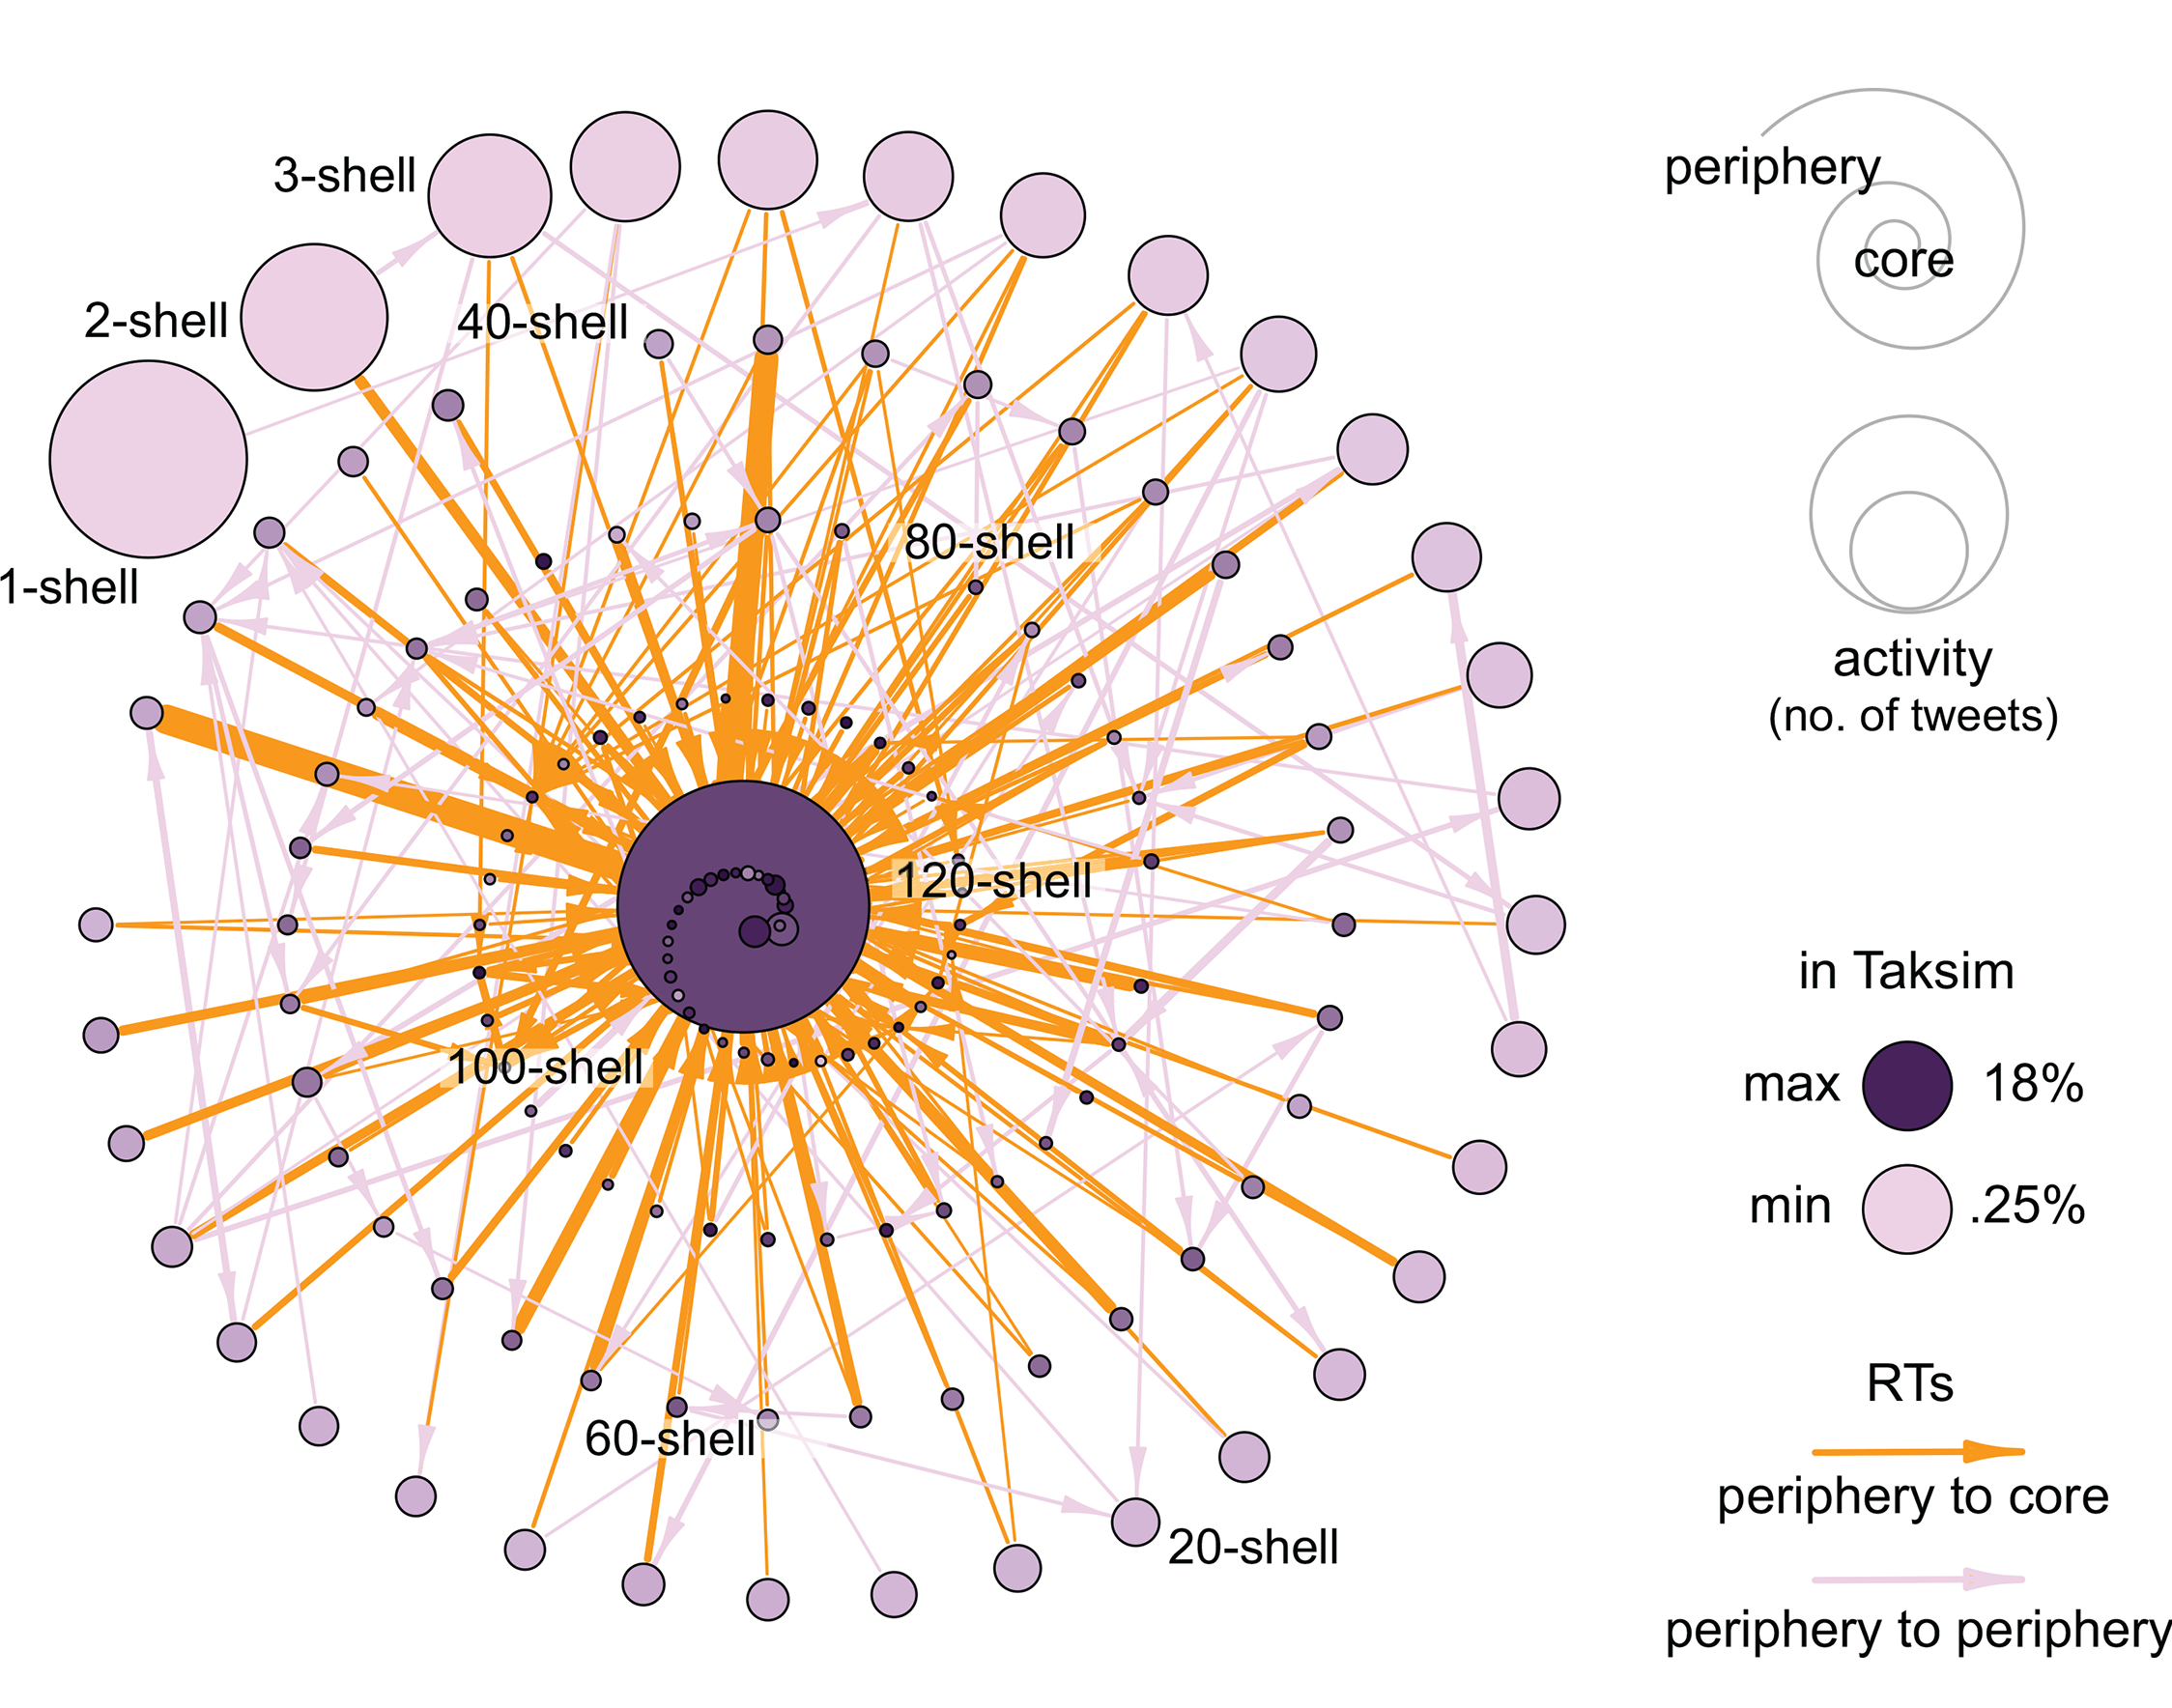
\includegraphics[scale=0.6]{Figures/VIS_taksim.png}
\caption{Diagrama de relaciones entre las \textit{k shells} de retweets de los participantes en las protestas del parque Taksim Gezi en Estamnul en 2013   \cite{barbera2015critical}.}
\label{fig:VIS_taksim}
\end{figure}


En el \textit{diagrama polar} se conservan las ideas de diagrama concéntrico y la coloración en función del \textit{k-shell}, pero hay cambios profundos en el resto de detalle. La naturaleza bipartita de las redes mutualistas es la principal diferencia con el \textit{fingerprint plot} original. En el diagrama polar cada clase ocupa uno de los semiplanos, divididos horizontalmente. La forma de los nodos se emplea para remarcar esta diferencia. 

El centro de cada especie se sitúa a una distancia $k_{radius}$ del origen de coordenadas. Recordemos que el valor mínimo de esta magnitud es $1$. El tamaño de los nodos es proporcional a su $k_{degree}$ y el color propio de la \textit{k-shell}. El algoritmo de representación asigna el ángulo que se distribuye para evitar al máximo la superposición de nodos. Una diferencia sustancial con el  \textit{fingerprint plot} es que en este tipo de visualizació no se representan los enlaces.

\begin{figure}[h!]
\centering
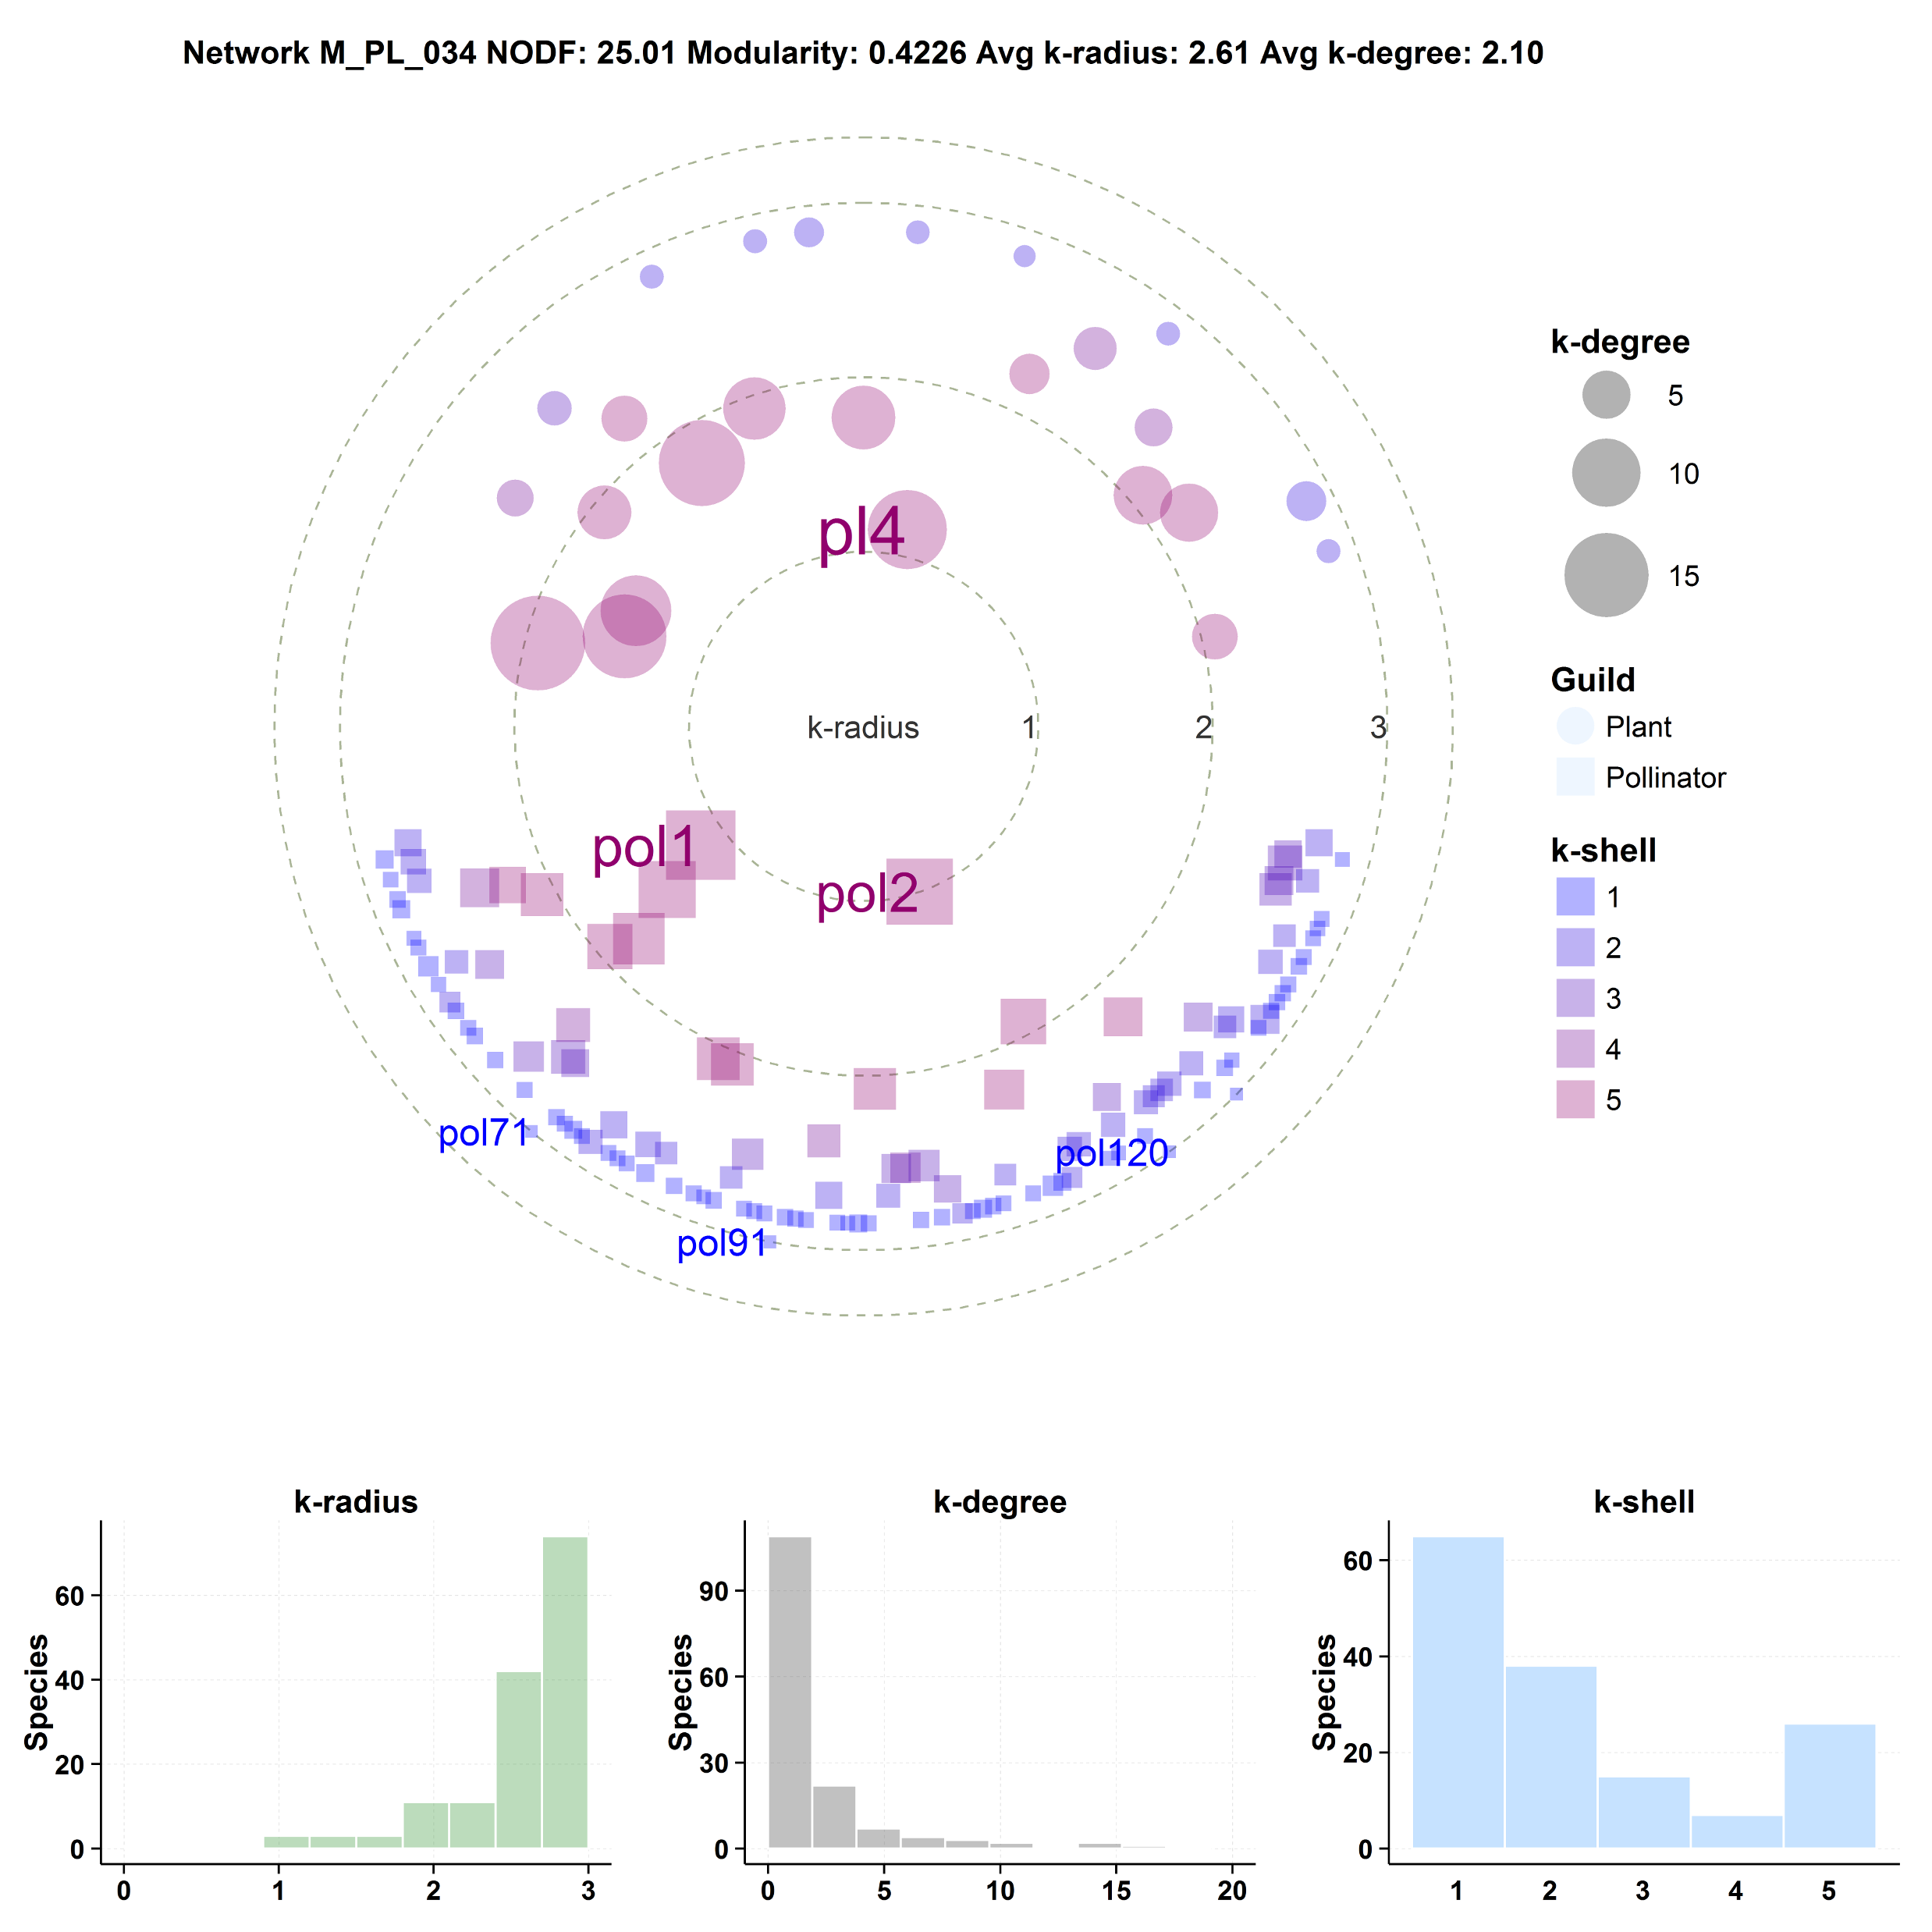
\includegraphics[scale=0.4]{Figures/VIS_M_PL_034_polar.png}
\caption[PolarExample]{Diagrama polar de una comunidad de polinizadores en la isla de Chiloé (Chile) \cite{smith2005diversity}.}
\label{fig:VIS_M_PL_034_polar}
\end{figure}

Se puede elegir incluir los nombres de todas las especies, de ninguna, o de un pequeño número, por defecto las tres más centrales y las tres más alejadas. Además, el usuario puede decidir que se añadan los histogramas de las tres \textit{k-magnitudes}, que contienen información muy valiosa.

La figura \ref{fig:VIS_M_PL_034_polar} es la representación polar de una red de polinizadores, que hemos elegido por ser una red mutualista tipo tanto por tamaño, anidamiento, modularidad y valores de las \textit{k magnitudes}, todos ellos no demasiado alejados de la media (tabla \ref{table:table_results}). El histograma de la distribución por \textit{k shells} tiene forma de bañera, muy repetido en estas redes. Hay unos pocos nodos dominantes y centrales, de índice $k = 5$ y un número importante de especies en las \textit{shells} exteriores. Es una red de elevada asimetría de especies ($0.66$), véase tabla \ref{table:table_results_recableados}).

La utilidad del diagrama polar se descubre al comparar varias redes, incluso si son de tamaños muy dispares. En la figura \ref{fig:VIS_Modvskdegree3}, se han escogido tres redes situadas en ambos extremos y en el centro del diagrama \ref{fig:ESTATICA_corrfigs} (derecha). La red de polinizadores $PL\_010$  tiene un valor de $Modularity$ bajo $(0.25)$, y alto el de $\overline {k}_{degree}$ $(4.57)$. El diagrama polar muestra la estructura en capas del mutualismo. Esta es mucho más evidente en la red $SD\_007$ ($Modularity: 0.28$, $\overline {k}_{degree}: 2.34$). La distribución de $\overline {k}_{degree}$ es más abrupta, con dos especies muy dominantes. La imagen transmite la idea de que esta red tiene una mayor organización jerárquica que $PL\_010$.

La red $PL\_021$ es grande y fuertemente modular ($Modularity: 0.57$, $\overline {k}_{degree}: 1.23$). La distribución de $\overline {k}_{degree}$ es aun más abrupta. Se ha incluido en la parte inferior izquierda la distribución de densidades que ya aparecía en la figura \ref{fig:ESTATICA_density_plots} porque la escala logarítmica en el eje horizontal permite ver mejor las diferencias.

\begin{figure}[h!]
\centering
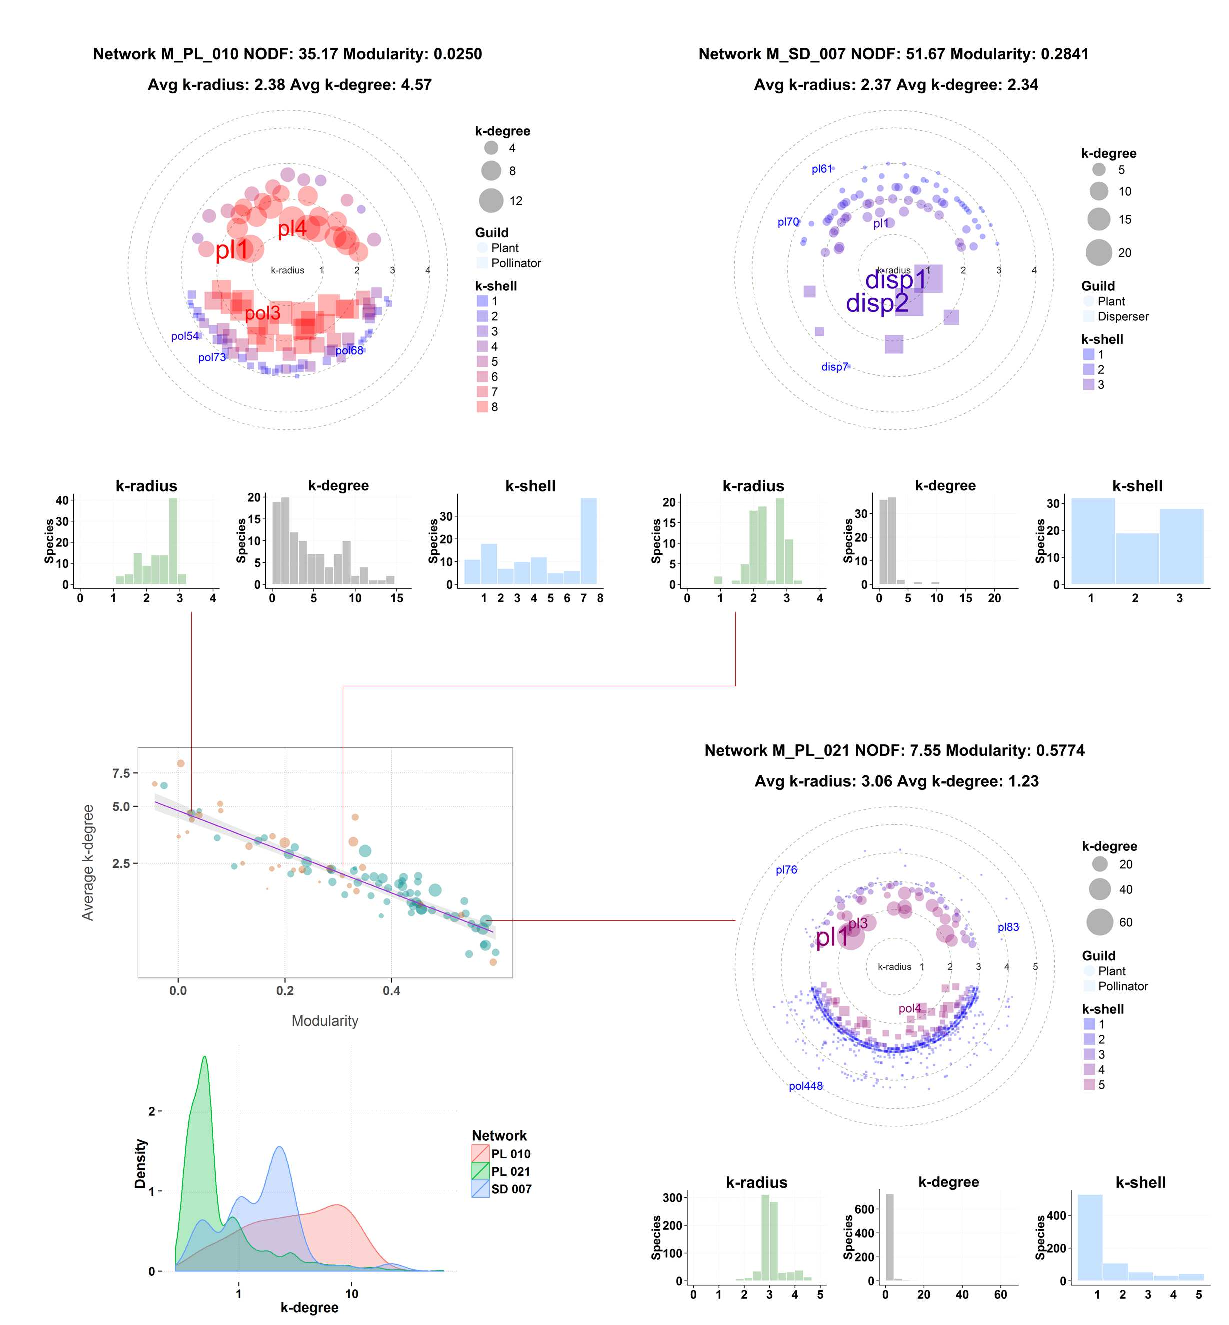
\includegraphics[scale=0.75]{Figures/VIS_Modvskdegree3.PDF}
\caption[PolarExample]{Comparación de tres redes mediante sus diagramas polares.}
\label{fig:VIS_Modvskdegree3}
\end{figure}

A pesar de que el diagrama polar ofrece una nueva visión de las comunidades mutualistas, tiene limitaciones. Como en toda estrategia de reducción de la información hay que renunciar a representar detalles en favor de una mejor visibilidad, en este caso los enlaces. No se trata de un detalle menor, así que se ha desarrollado un segundo tipo de diagrama que los toma como base de su construcción.

\clearpage
\subsection{El diagrama zigurat}
\label{sec:diagrama_zigurat}

El diagrama zigurat se ha creado para mostrar la estructura de \textit{k shells} de una red bipartita y los enlaces entre sus nodos. La idea básica consiste en agrupar las especies en \textit{shells} que se representan como pequeños zigurats\footnote{Según el DRAE: Torre escalonada y piramidal, característica de la arquitectura religiosa asiria y caldea.}. Las dos \textit{shells} máximas se colocan en el eje de simetría horizontal, ligeramente hacia la izquierda. El resto, se distribuyen siguiendo una disposición en forma de almendra, que deja un gran espacio libre para dibujar los enlaces.

\begin{figure}[h!]
\centering
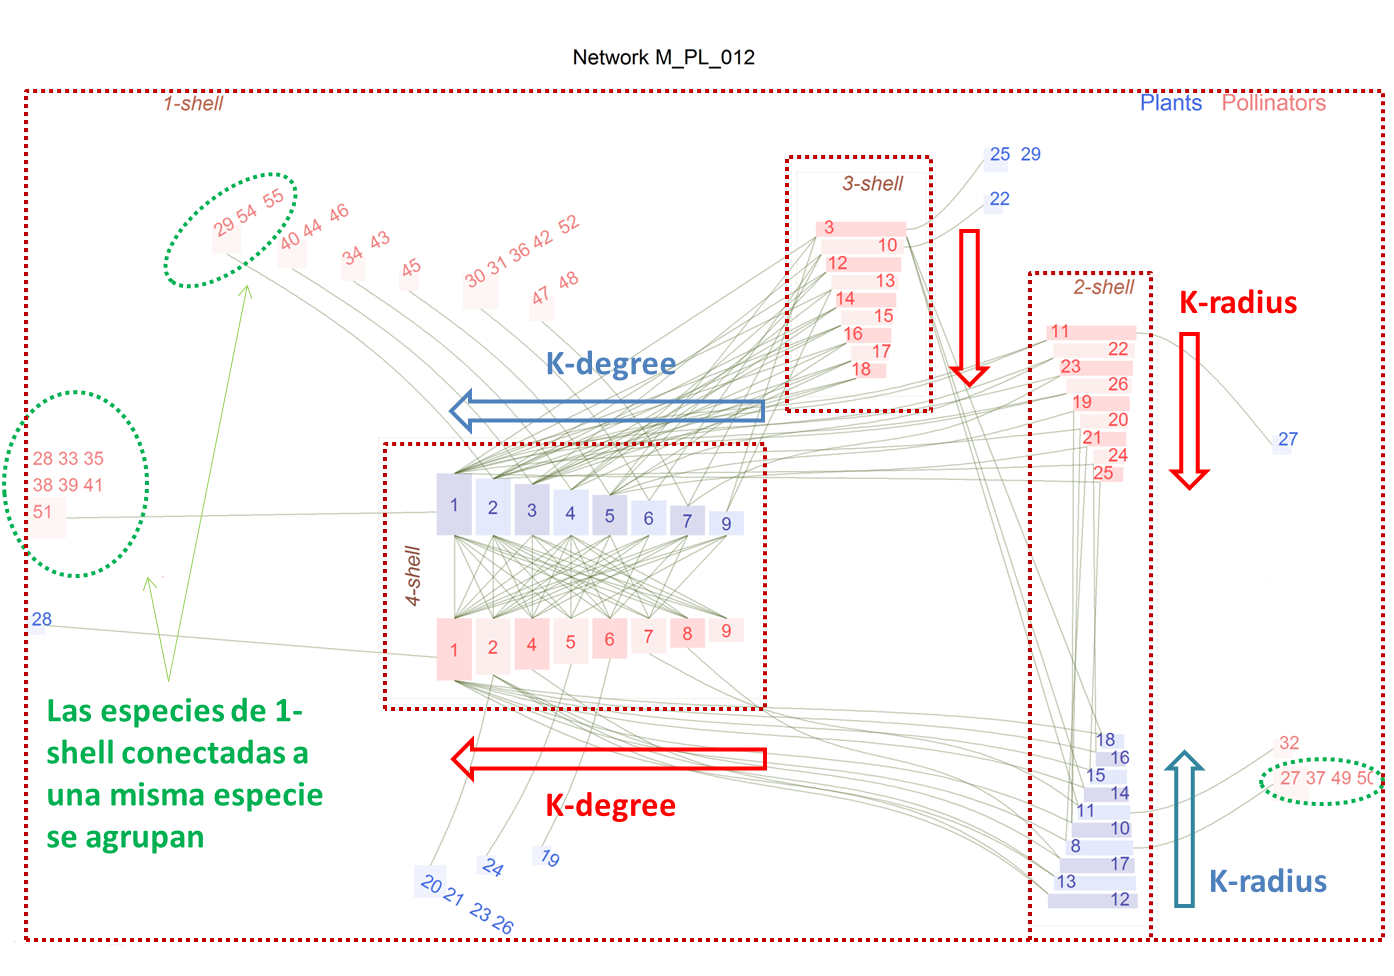
\includegraphics[scale=0.4]{Figures/VIS_explicacion_zigurat.png}
\caption {Estructura del diagrama zigurat para la red  $M\_PL\_012$.}
\label{fig:VIS_explicacion_zigurat}
\end{figure}

Las clases se diferencian por el color de relleno. Para cada una se emplean dos tonalidades del mismo color lo que facilita la lectura del diagrama. Las especies se indican por el número
con el que figuran en el fichero de datos, de $1$ a $m$ para una clase y de $1$ a $n$ para la otra.

En la \textit{shell} máxima las especies se ordenan por $k_{degree}$, con el valor mayor en el extremo izquierdo. Esta disposición facilita la colocación a su altura del grupo de especies de la $1$-$shell$ con las que se conecta, que pueden llegar a ser muy numerosas. En el resto de \textit{shell}, las especies se ordenan por $k_{radius}$, correspondiendo la base del zigurat a la de menor $k_{radius}$.

\begin{figure}[hb!]
\centering
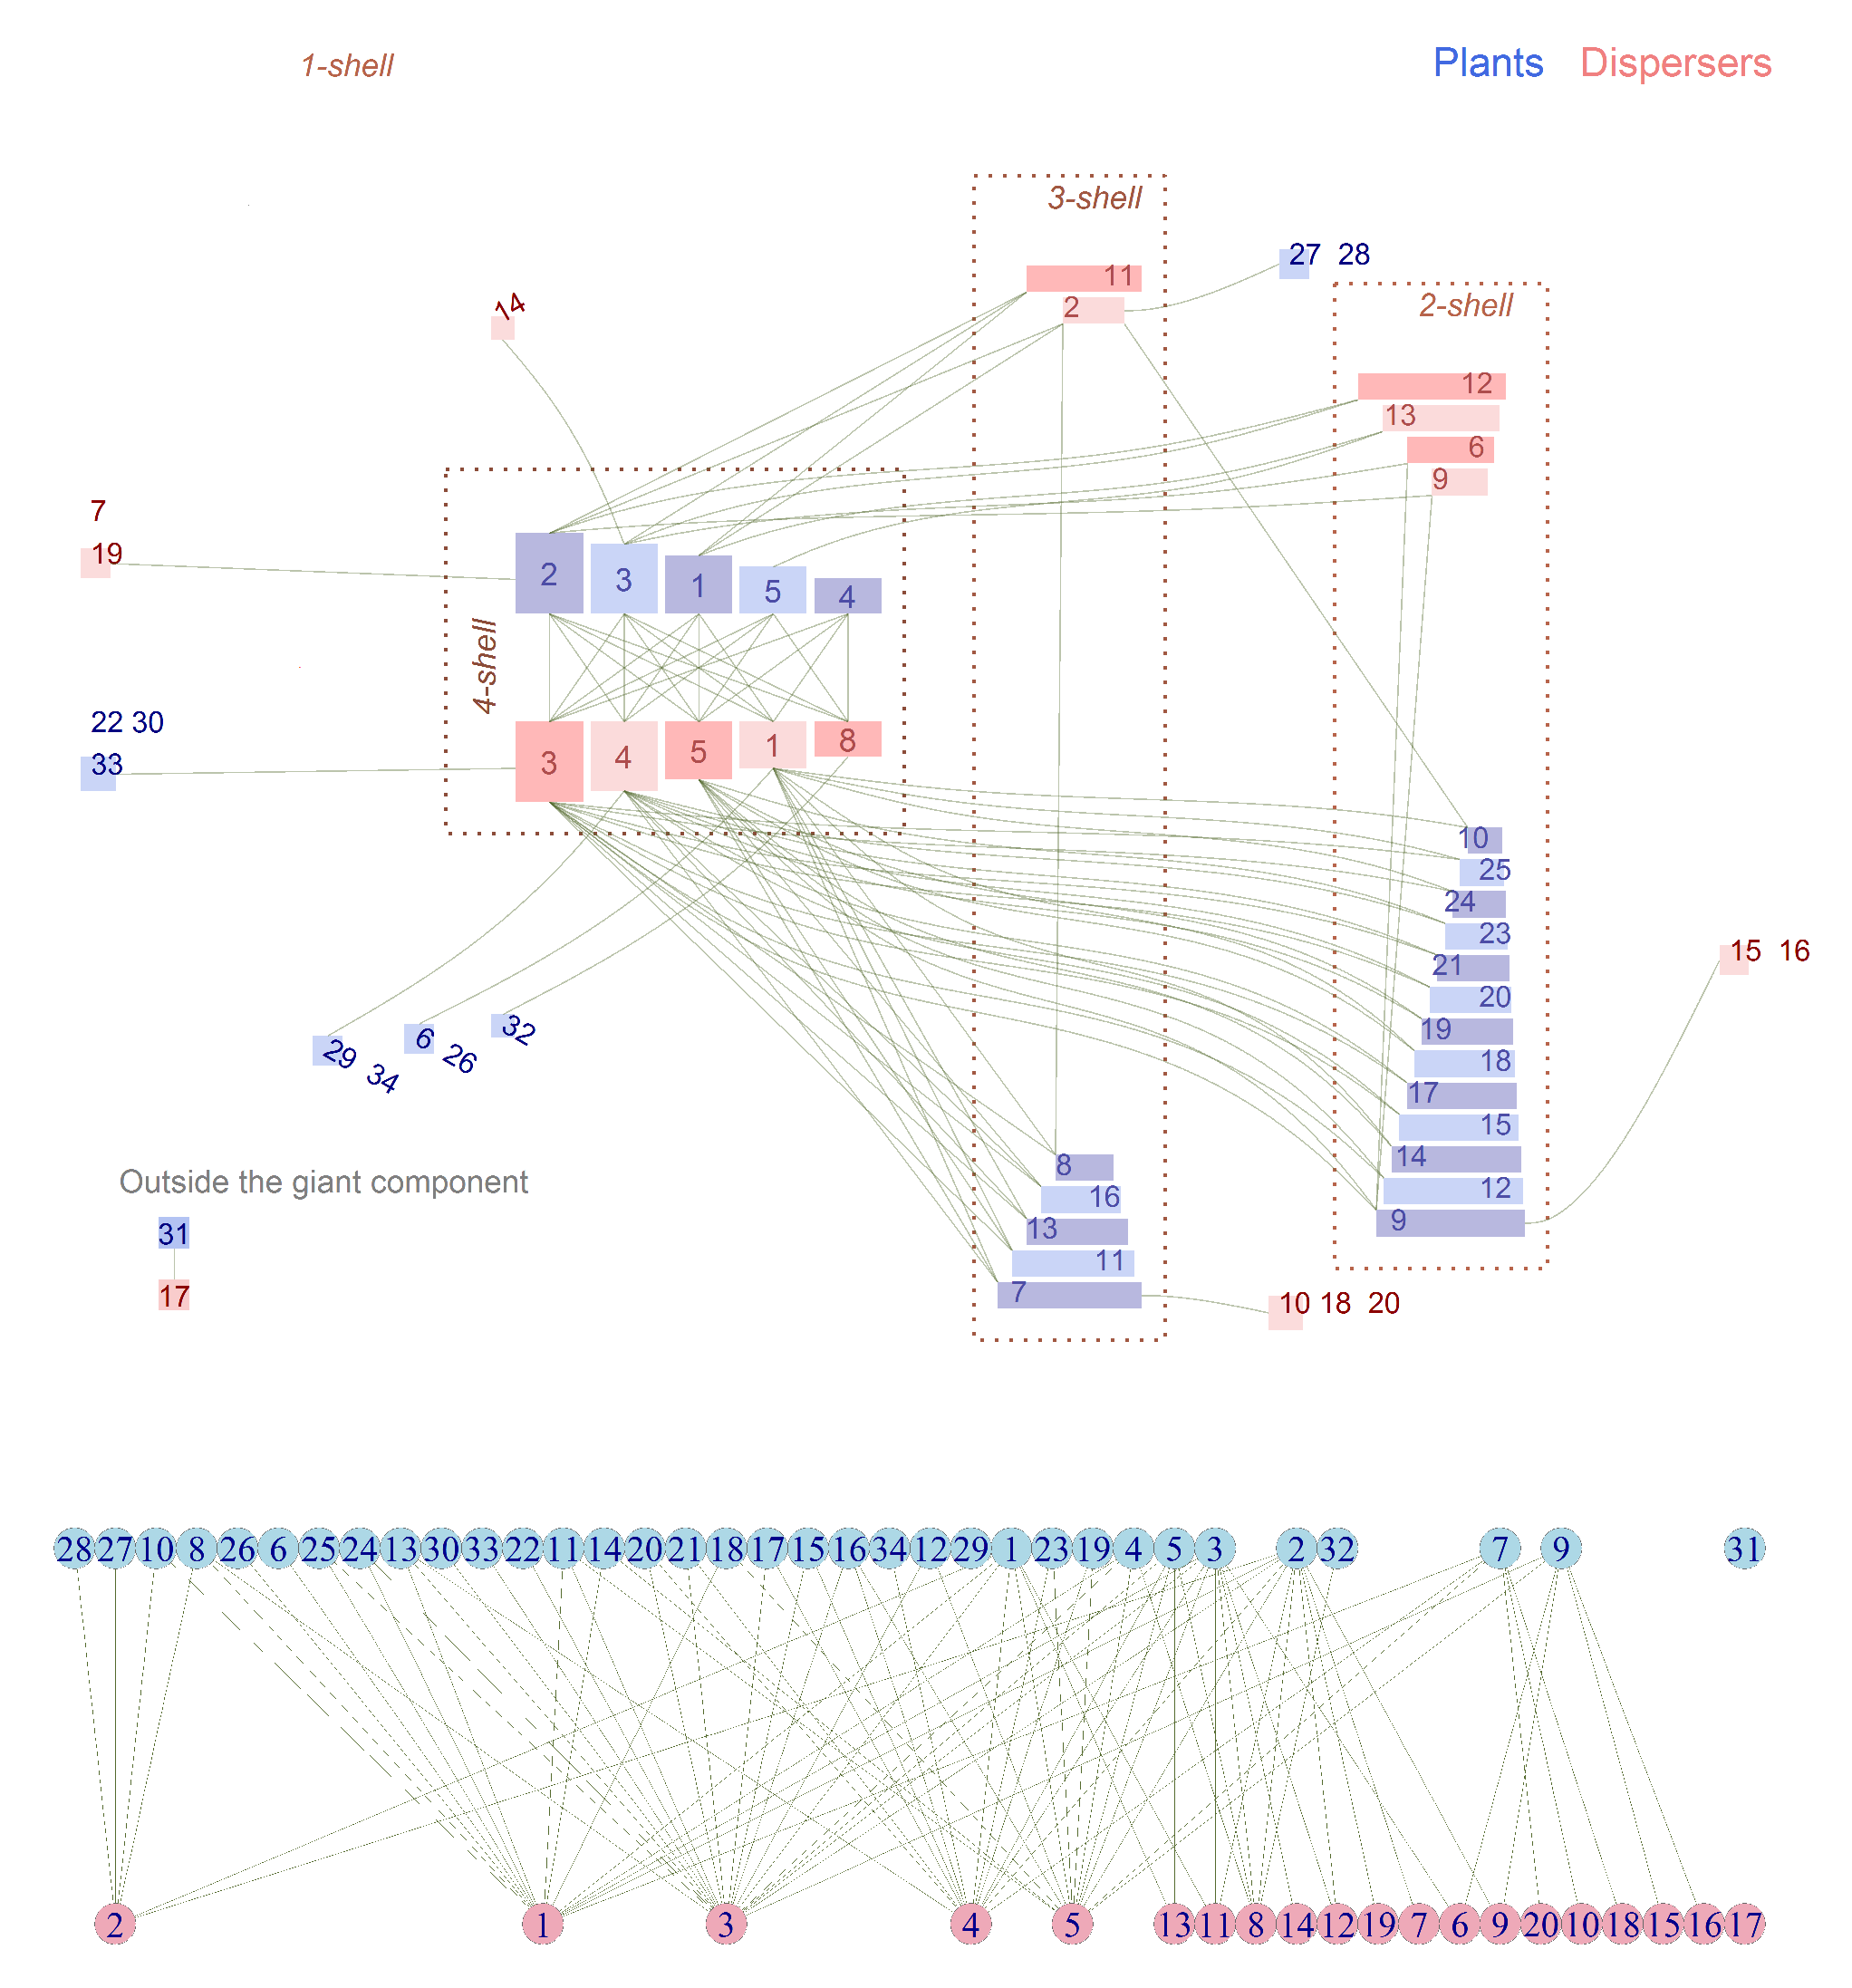
\includegraphics[scale=0.45]{Figures/VIS_ALL_SD_004.eps}
\caption {Diagrama zigurat de una comunidad de aves frugívoras de Puerto Rico  $M\_SD\_004$, con $54$ especies y $95$ enlaces \cite{carlo2003avian}. $\overline k_{radius} = 2,19$; $\overline k_{degree} = 2,37$; $NODF = 39,82$; $Modularity = 0.34$. Abajo el diagrama bipartito.}
\label{fig:ziggurat}
\end{figure}

Los enlaces entre especies de la \textit{shell} máxima se representan entre las bases de sus rectángulos. El enlace entre dos especies de \textit{shells} de distinto índice conecta el lado izquierdo de la de índice inferior y el derecho de la de la de índice superior, salvo que sea la máxima, en cuyo caso se usa el extremo superior. Los enlaces entre especies de la misma \textit{shell} conectan los extremos izquierdos de ambas.

Las especies de la $1$-$shell$ se disponen como una nube el torno a los zigurats de la almendra central. Si, como sucede a menudo, varias especies de esta \textit{shell} comparten la única especie con la que se conectan, se dibujan de forma agrupada y con un único enlace. Puede verse en los ejemplos dentro de las elipses punteadas en verde de la figura \ref{fig:VIS_explicacion_zigurat}. Pueden distinguirse las tres ubicaciones características de estos grupos: a la izquierda de la \textit{k shell} máxima (para los conectados a la especie de mayor $k_{degree}$), encima del resto de las especies de esta \textit{shell} y a la derecha de los demás zigurats.


En algunas redes se incluyen observaciones de especies que no están conectadas con la componente gigante. En ese caso, se representa el fragmento inconexo, pero no se tiene en cuenta para la \textit{k descomposición}.

Un detalle importante es que en el diagrama zigurat, las áreas no transmiten información. Se han dispuesto así por conveniencia para poder representar con la mayor claridad posible los enlaces y las agrupaciones en \textit{k shells}.

La red de la figura \ref{fig:ziggurat} es de pequeño tamaño y produce una figura que recuerda a un pez con su boca y aletas. Esta imagen se repite en numerosos ejemplos. En el gráfico bipartito todavía se pueden seguir los enlaces individuales. Sin embargo, el zigurat ofrece una visión mucho más rica de la organización con cuatro \textit{shells} internas y la $1$-$shell$ con pocas especies. Se pueden descubrir con facilidad algunos patrones, como la baja conectividad entre especies de las \textit{shells} de menor índice $k$, o la relativa importancia de la especie dispersora $2$ que en el bipartito aparece en el extremo izquierdo. Hay dos especies desconectadas de la componente gigante, pueden verse en la parte inferior izquierda del diagrama.

\begin{figure}[hp!]
\centering
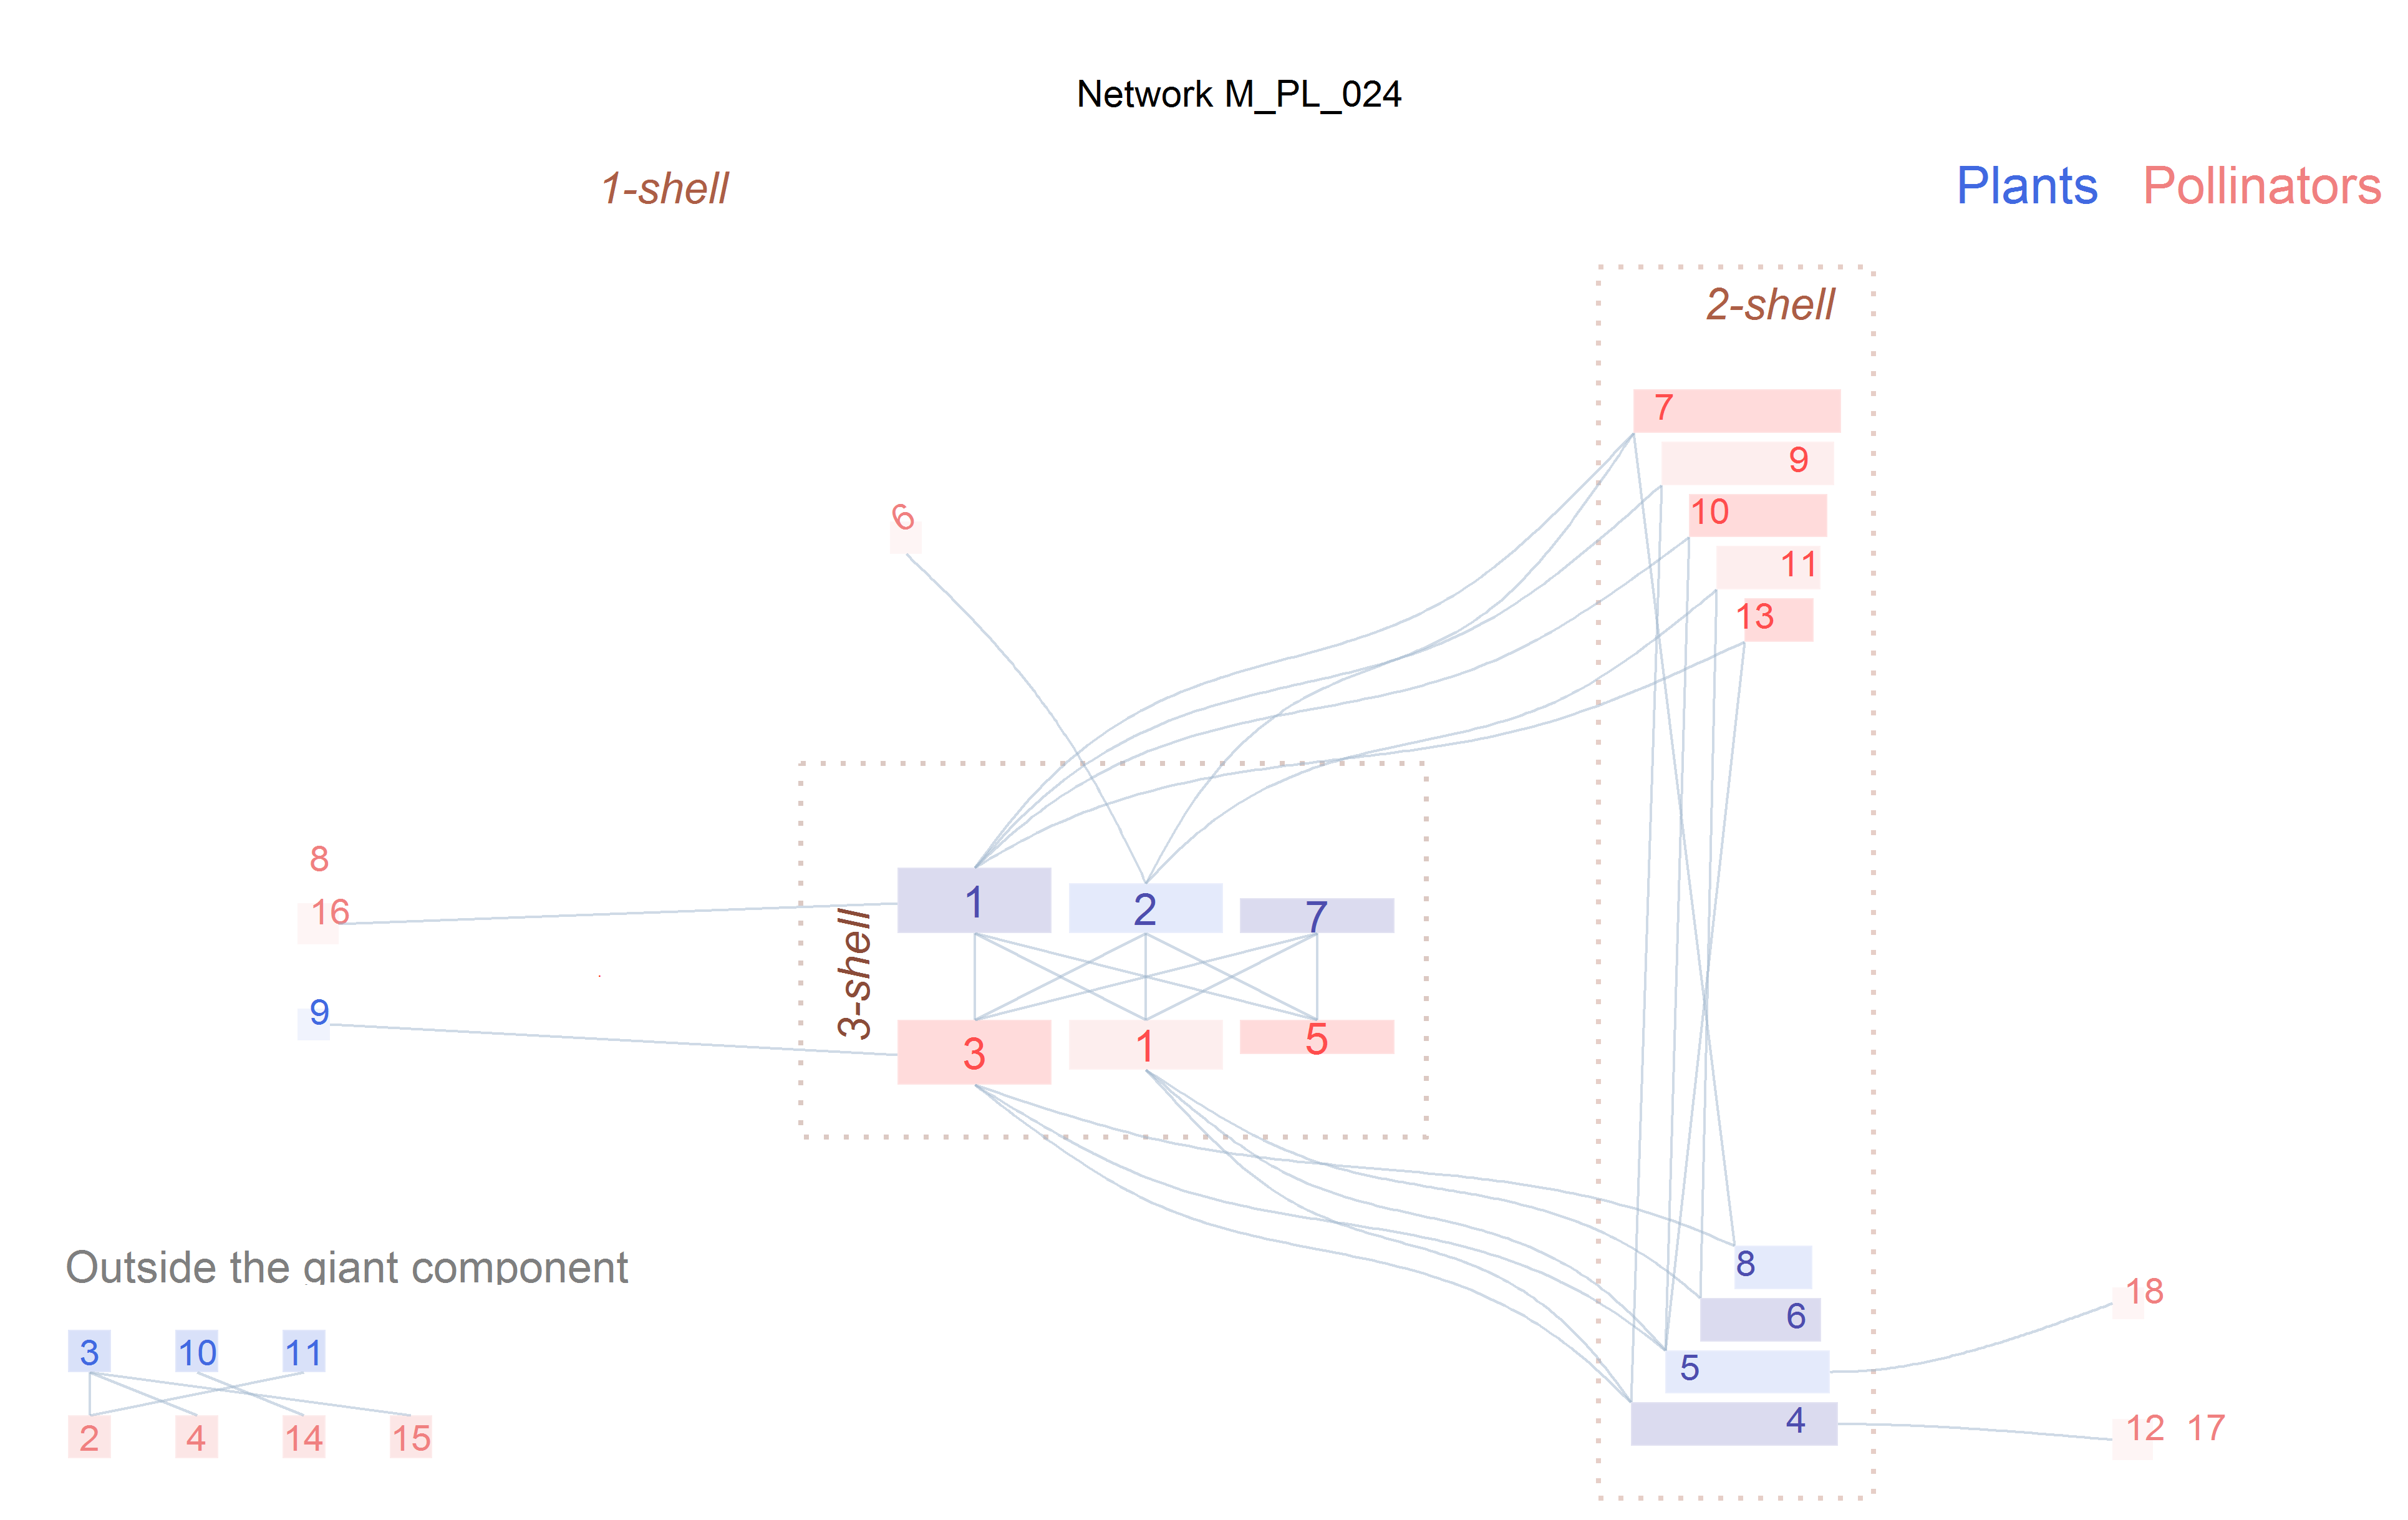
\includegraphics[scale=0.45]{Figures/VIS_M_PL_024_ziggurat.png}
\caption {Red de polinizadores $M\_PL\_024$, Melville Island, Canadá \cite{mosquin1967observations}, con $29$ especies y $38$ enlaces}
\label{fig:VIS_zig_pl_024}
\end{figure}

El diagrama zigurat funciona bien para los tamaños típicos de las redes mutualistas documentadas en la literatura. La red de la figura \ref{fig:VIS_zig_pl_024} es pequeña, muy simétrica y con valores intermedios de $NODF$ y de las \textit{k magnitudes} (véase la tabla \ref{table:table_results}). La especie con mayor $k_{degree}$ $(5,74)$ es la planta $1$. En esta red todas las especies de las \textit{shells} máximas están conectadas entre sí, por lo que sus $k_{radius}$ valen $1,0$, pero esto no tiene por qué suceder siempre. Las más distantes de la $3$-$shell$ (descartando las que no están conectadas con la componente gigante) son los polinizadores $12$, $17$ y $18$, con  $k_{radius}$ $3,0$, que aparecen conectadas al extremo derecho del zigurat de la $2$-$shell$ de plantas.

\begin{figure}[h!]
\centering
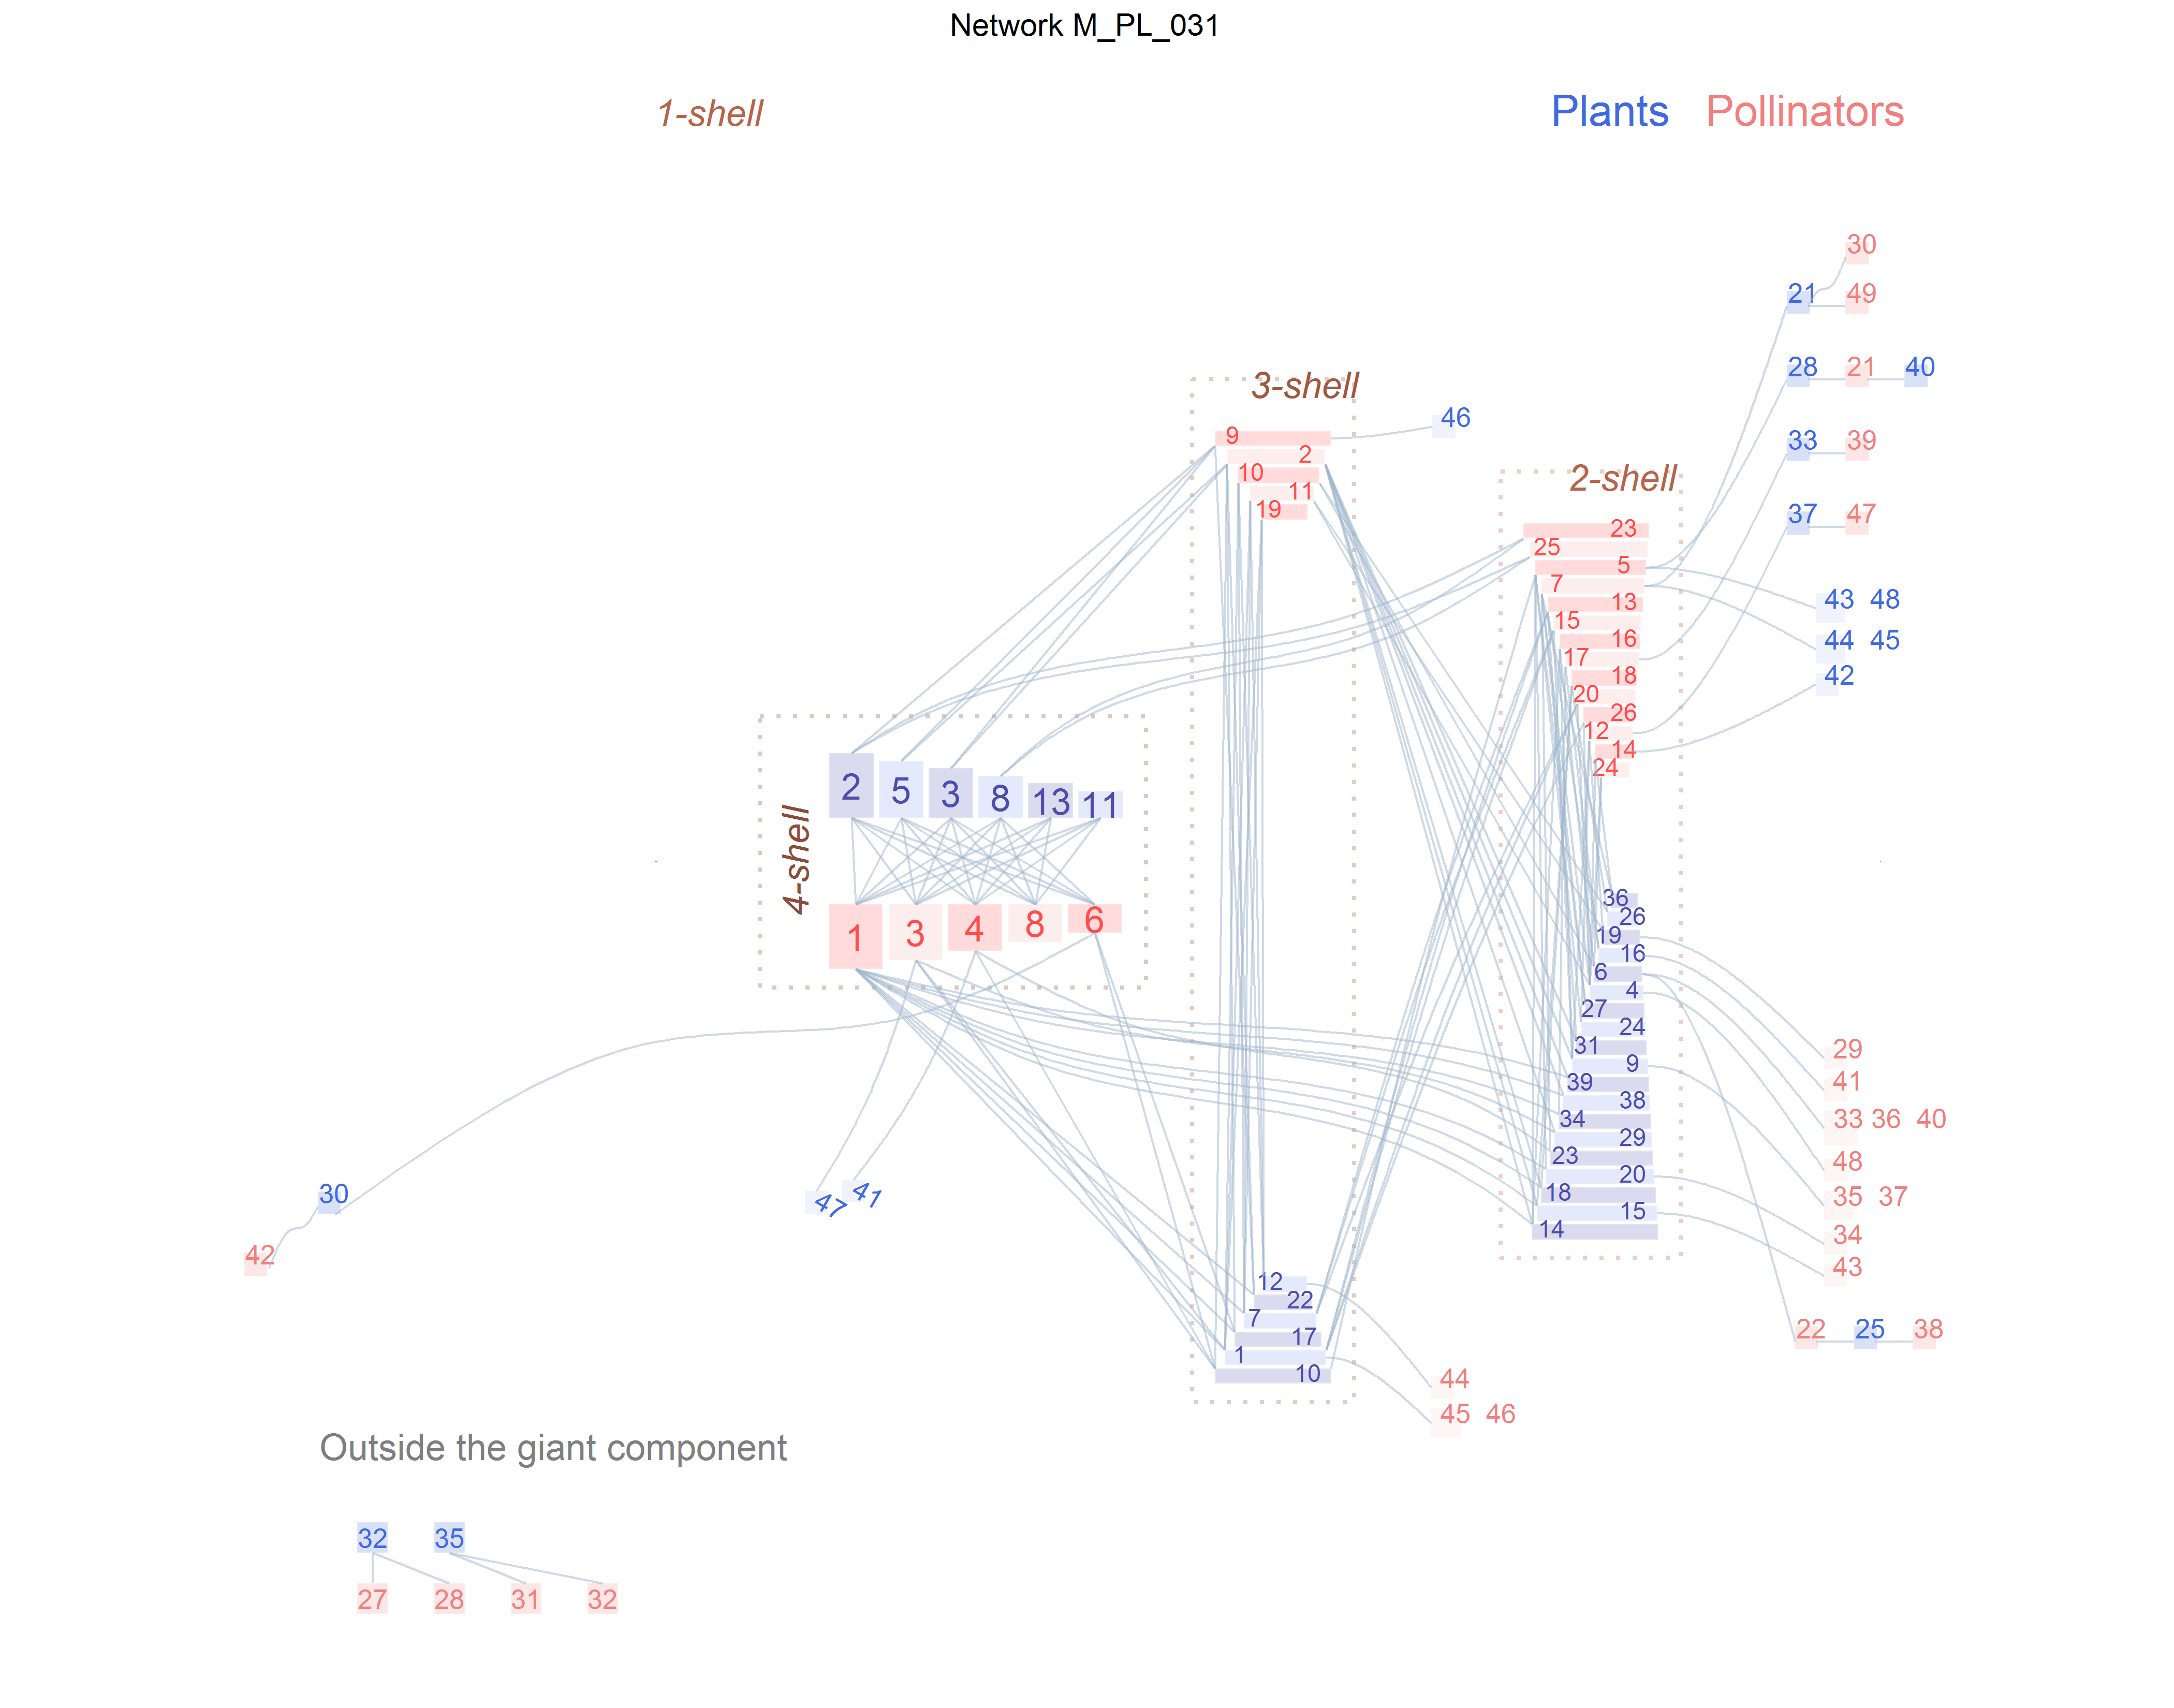
\includegraphics[scale=1]{Figures/VIS_M_PL_031_ziggurat.png}
\caption {Red de polinizadores $M\_PL\_031$ del Parque Nacional de Canaima, Venezuela, con $97$ especies y $156$ enlaces \cite{ramirez1989biologia}.}
\label{fig:VIS_M_PL_031_ziggurat}
\end{figure}

La red de la figura \ref{fig:VIS_M_PL_031_ziggurat} es de un tamaño intermedio, y muestra abundancia de especialistas conectadas a otras especialistas, una circunstancia poco común. A diferencia del caso anterior, no todas las especies del las \textit{shells} máximas tienen enlaces directos con todas las de la clase contraria. Así, mientras el $k_{radius}$ del polinizador $1$ o la planta $2$ es $1,0$, el de la planta $13$ es $1,4$ y el del polinizador $6$ es $1.66$ (tabla \ref{table:kmag_pl_031}). La existencia de especialistas ultraperiféricos se traduce en valores elevados del $k_{radius}$, por ejemplo $7.0$ para el polinizador $38$ ó $6.2$ para la planta $25$ que es el primer enlace de su camino más corto hacia el centro de la red.

\begin{figure}[ht!]
\centering
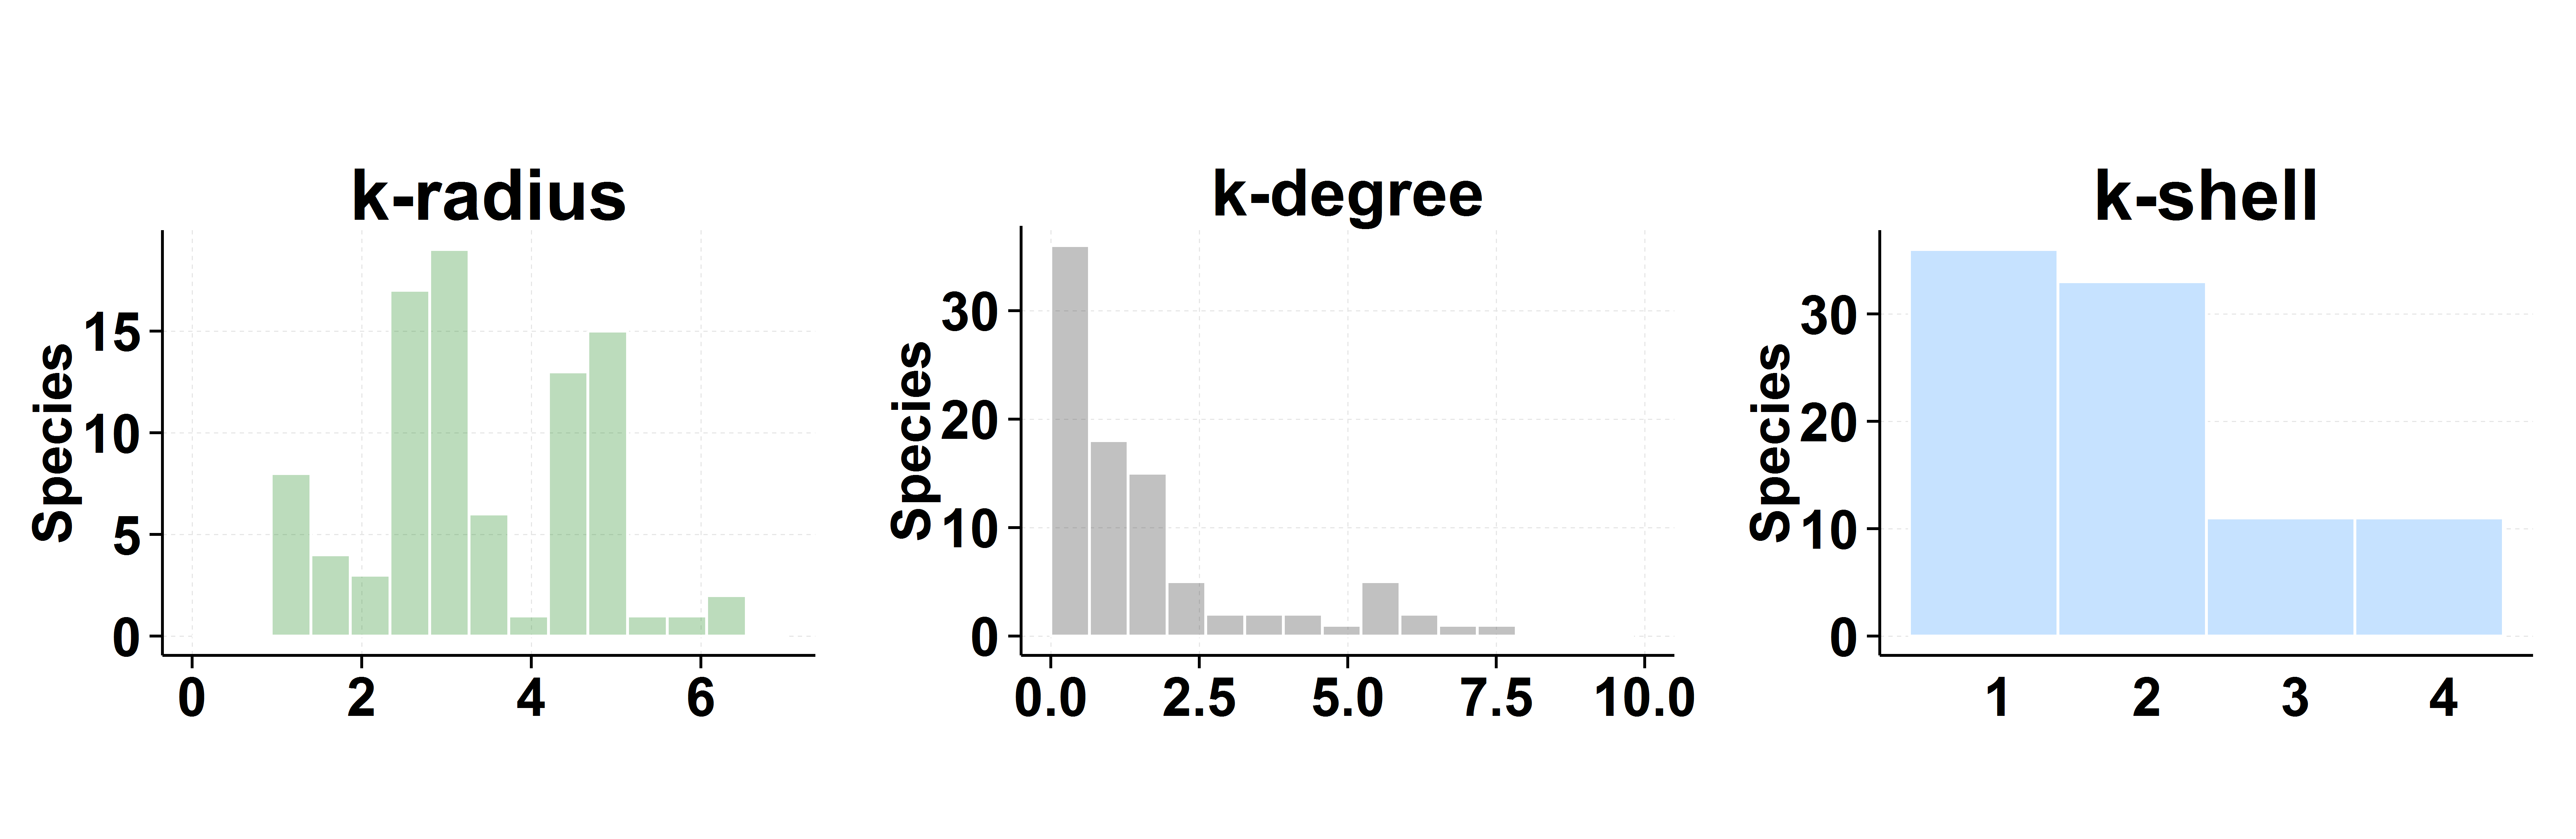
\includegraphics[scale=0.5]{Figures/VIS_M_PL_031_polar.png}
\caption {Histograma de las \textit{k magnitudes} de polinizadores del Parque Nacional de Canaima, Venezuela \cite{ramirez1989biologia}.}
\label{fig:VIS_M_PL_031_polar}
\end{figure}

Estas especies tan alejadas del centro corren el peligro de extinción por arrastre que se describió en el apartado \ref{results_K_constante}. Supongamos que el polinizador número $7$ se extingue por una plaga. En la parte superior derecha de la figura \ref{fig:VIS_M_PL_031_ziggurat} puede verse la tripleta planta $21$, polinizadores $30$ y $49$ que quedarían desconectados de la componente gigante y posiblemente se extinguirían también. En el mejor de los casos, si por el peso de sus enlaces superaran el mínimo vital de la nueva red formada por las tres, podrían sobrevivir aisladas pero mucho más expuestas a cualquier perturbación posterior. Las plantas $44$ y $45$ desaparecerían con seguridad porque el polinizador $7$ es su única especie benefactora. De esta manera, la destrucción de un polinizador podría arrastrar cinco especies más a la extinción. En el diagrama se puede ver también la gran conectividad entre especies de las \textit{shells} de índices $2$ y $3$, lo que reduce el anidamiento bajo y aumenta la modularidad. Por el contrario, la red de la figura \ref{fig:ziggurat} es mucho más anidada, con pocos enlaces que no terminen en la $4$-$shell$ y compacta, con un $\overline k_{radius}$ reducido ($2,19$ frente a $3,39$).


El tamaño de una red se puede medir en número de nodos o en número de enlaces, pero es esta segunda cifra la que predomina a la hora de fijar la complejidad de la estructura de \textit{k shells}. La red de la figura \ref{fig:VIS_M_PL_010_ziggurat}, tiene $107$ especies y $456$ enlaces y su índice $k$ máximo es $8$. Se aprecia asimetría importante con predominio de los polinizadores. En contraste con los ejemplos anteriores, hay muy pocas especies que pertenezcan a la $1$-$shell$. Las conexiones entre las distintas \textit{shells} forman un entramado visualmente complejo.

Con menos especies $(85)$ y solo un $10\%$ más de enlaces, la comunidad de frugívoros de la selva malaya de la figura \ref{fig:VIS_M_PL_047_ziggurat}, tiene un índice $k$ máximo de $11$, ninguna otra de la colección \textit{web of life} lo alcanza. Es muy asimétrica y el valor de $\overline k_{degree}$ es excepcional ($8,4$), por la circunstancia de tener ese $k$ máximo, la elevada conectividad de las especies y su cercanía a la $11$-$shell$.

La red de polinizadores de un brezal danés (figura \ref{fig:VIS_M_PL_047_ziggurat}), tiene $205$ especies y $425$ enlaces. El $k$ máximo es solo $6$. La asimetría es también muy marcada pero lo que más destaca es la extraordinaria cantidad de polinizadores en la $1$-$shell$. Con este ejemplo se aprecia mejor el valor de agrupar todas las especies de la $1$-$shell$ que se conectan a una especie de las \textit{shells} más internas y dibujar solo un enlace. 

\begin{figure}[ht!]
\centering
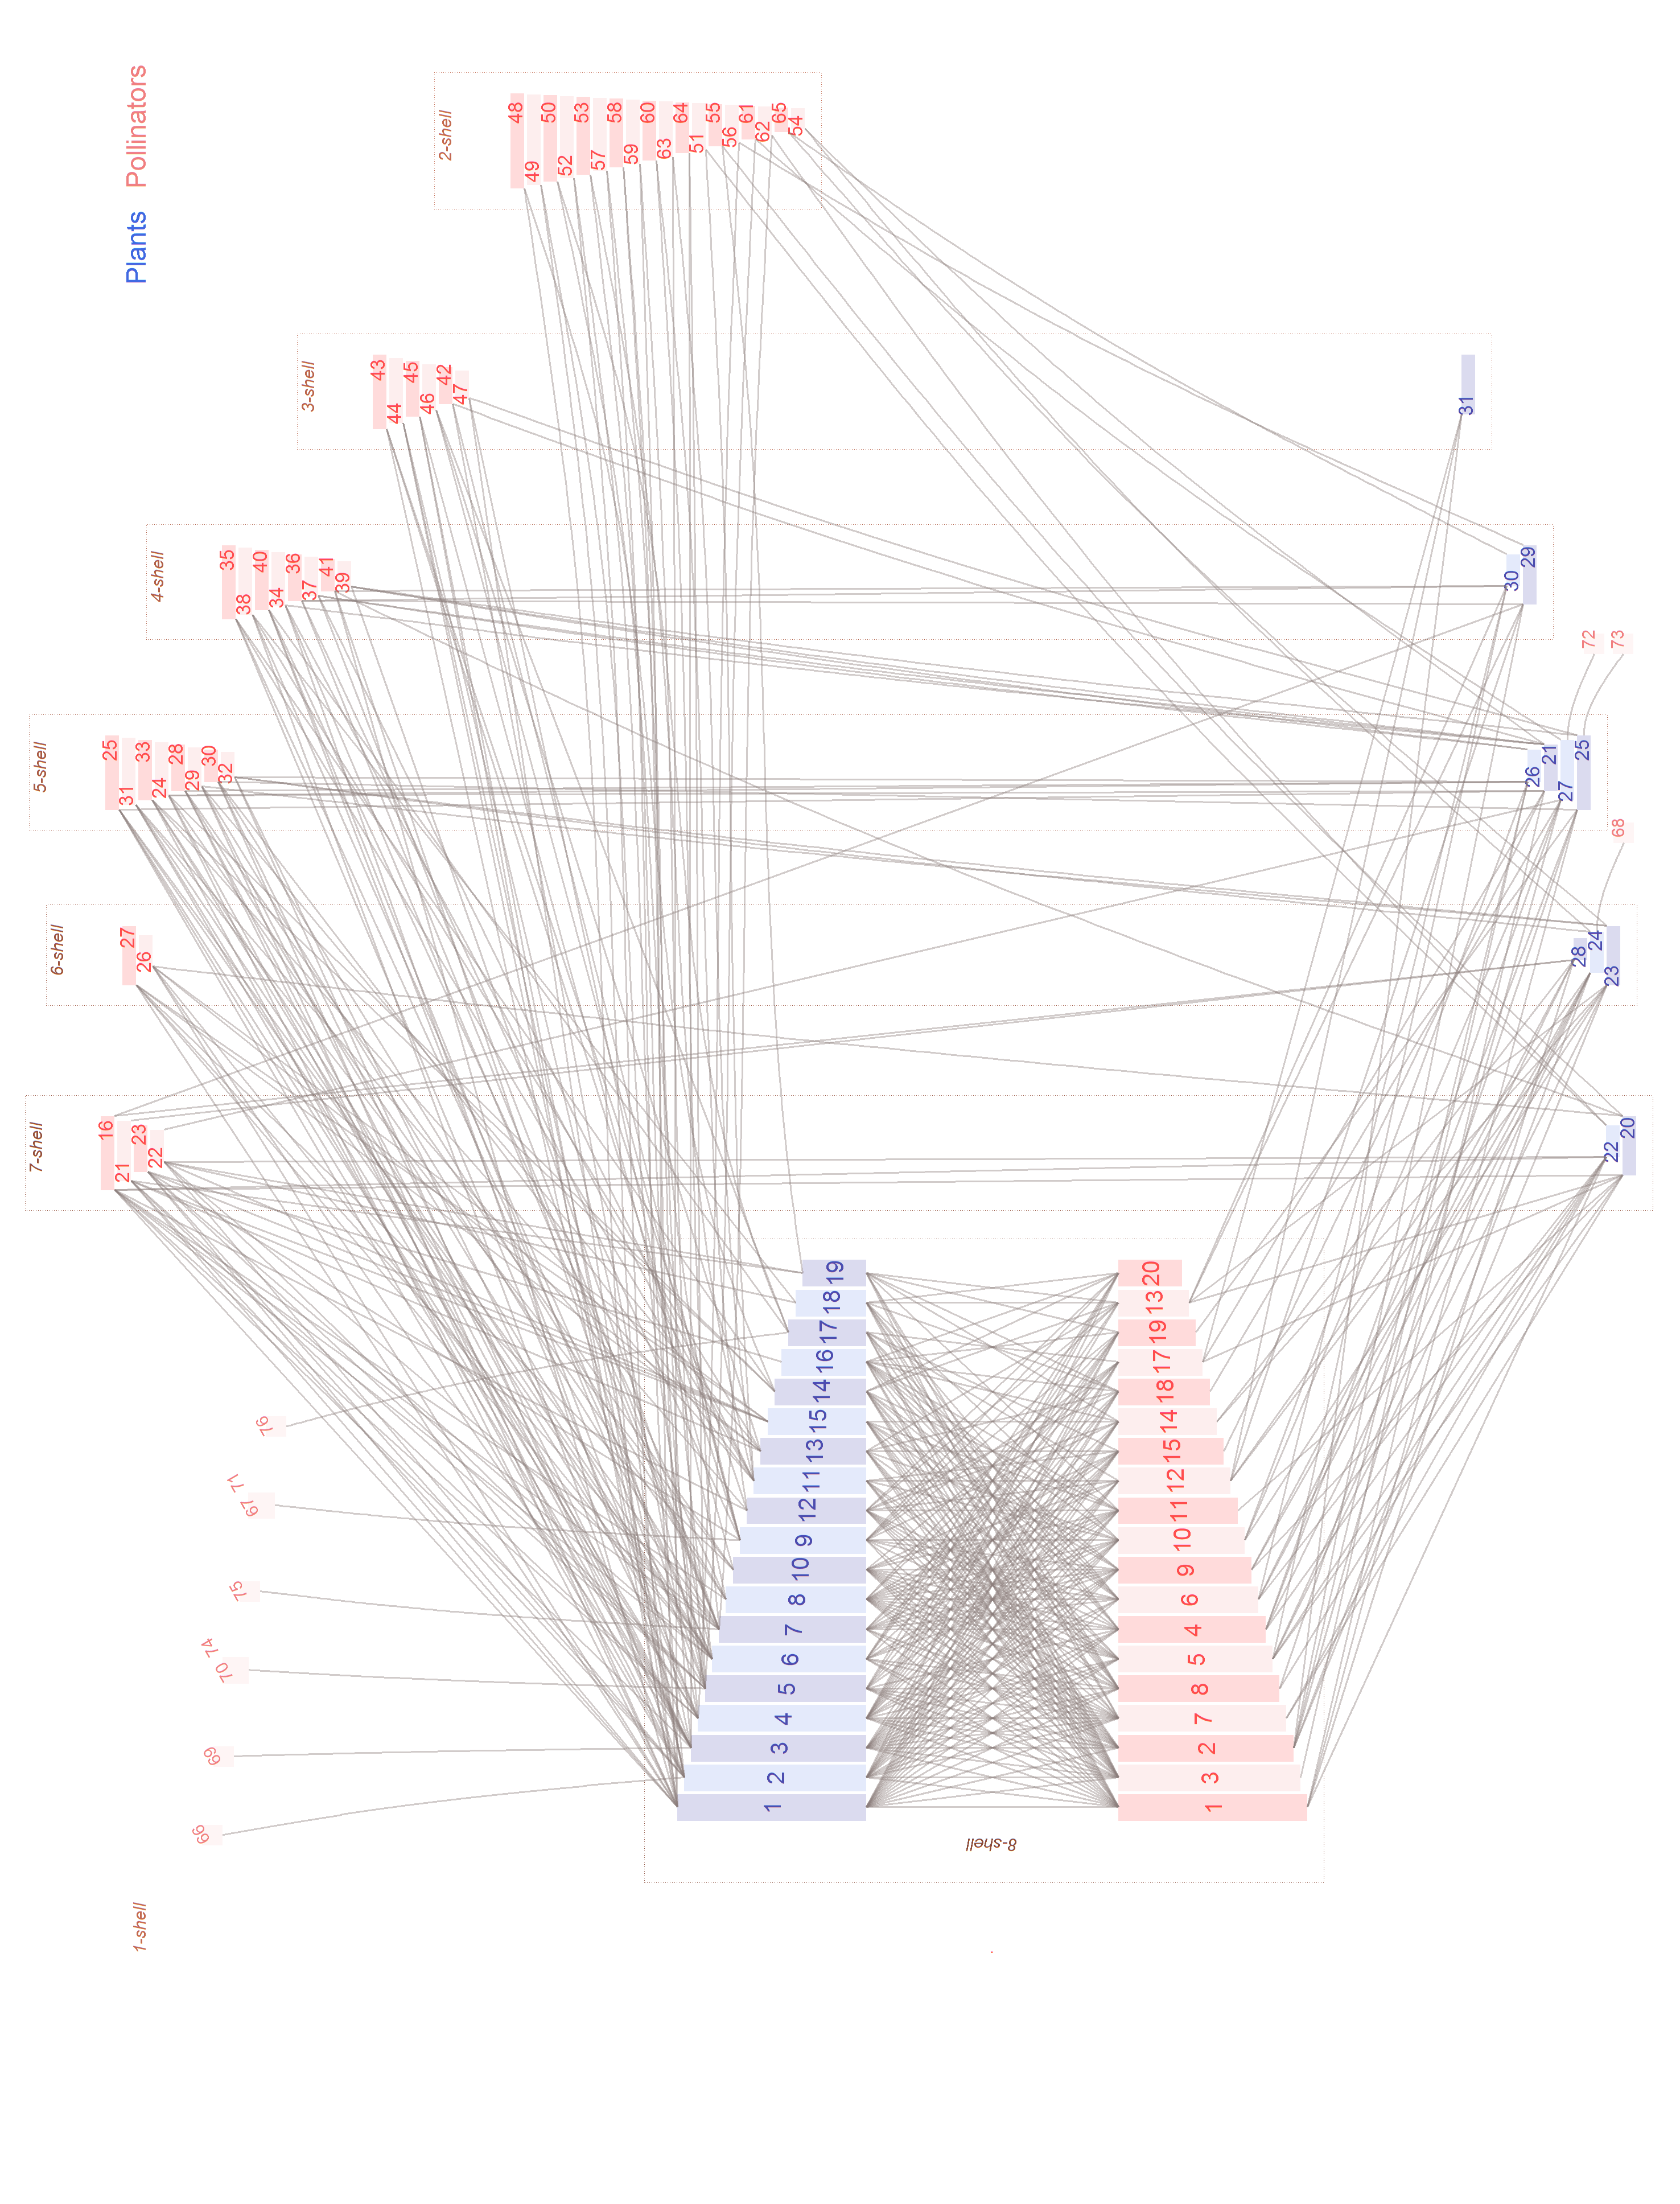
\includegraphics[scale=0.5]{Figures/VIS_M_PL_010_ziggurat.png}
\caption {Red de polinizadores $M\_PL\_010$ (Elberling \& Olesen, no publicada), con $107$ especies y $456$ enlaces. Su diagrama polar puede verse en la figura \ref{fig:VIS_Modvskdegree3}.}
\label{fig:VIS_M_PL_010_ziggurat}
\end{figure}

\clearpage
\begin{figure}[ht!]
\centering
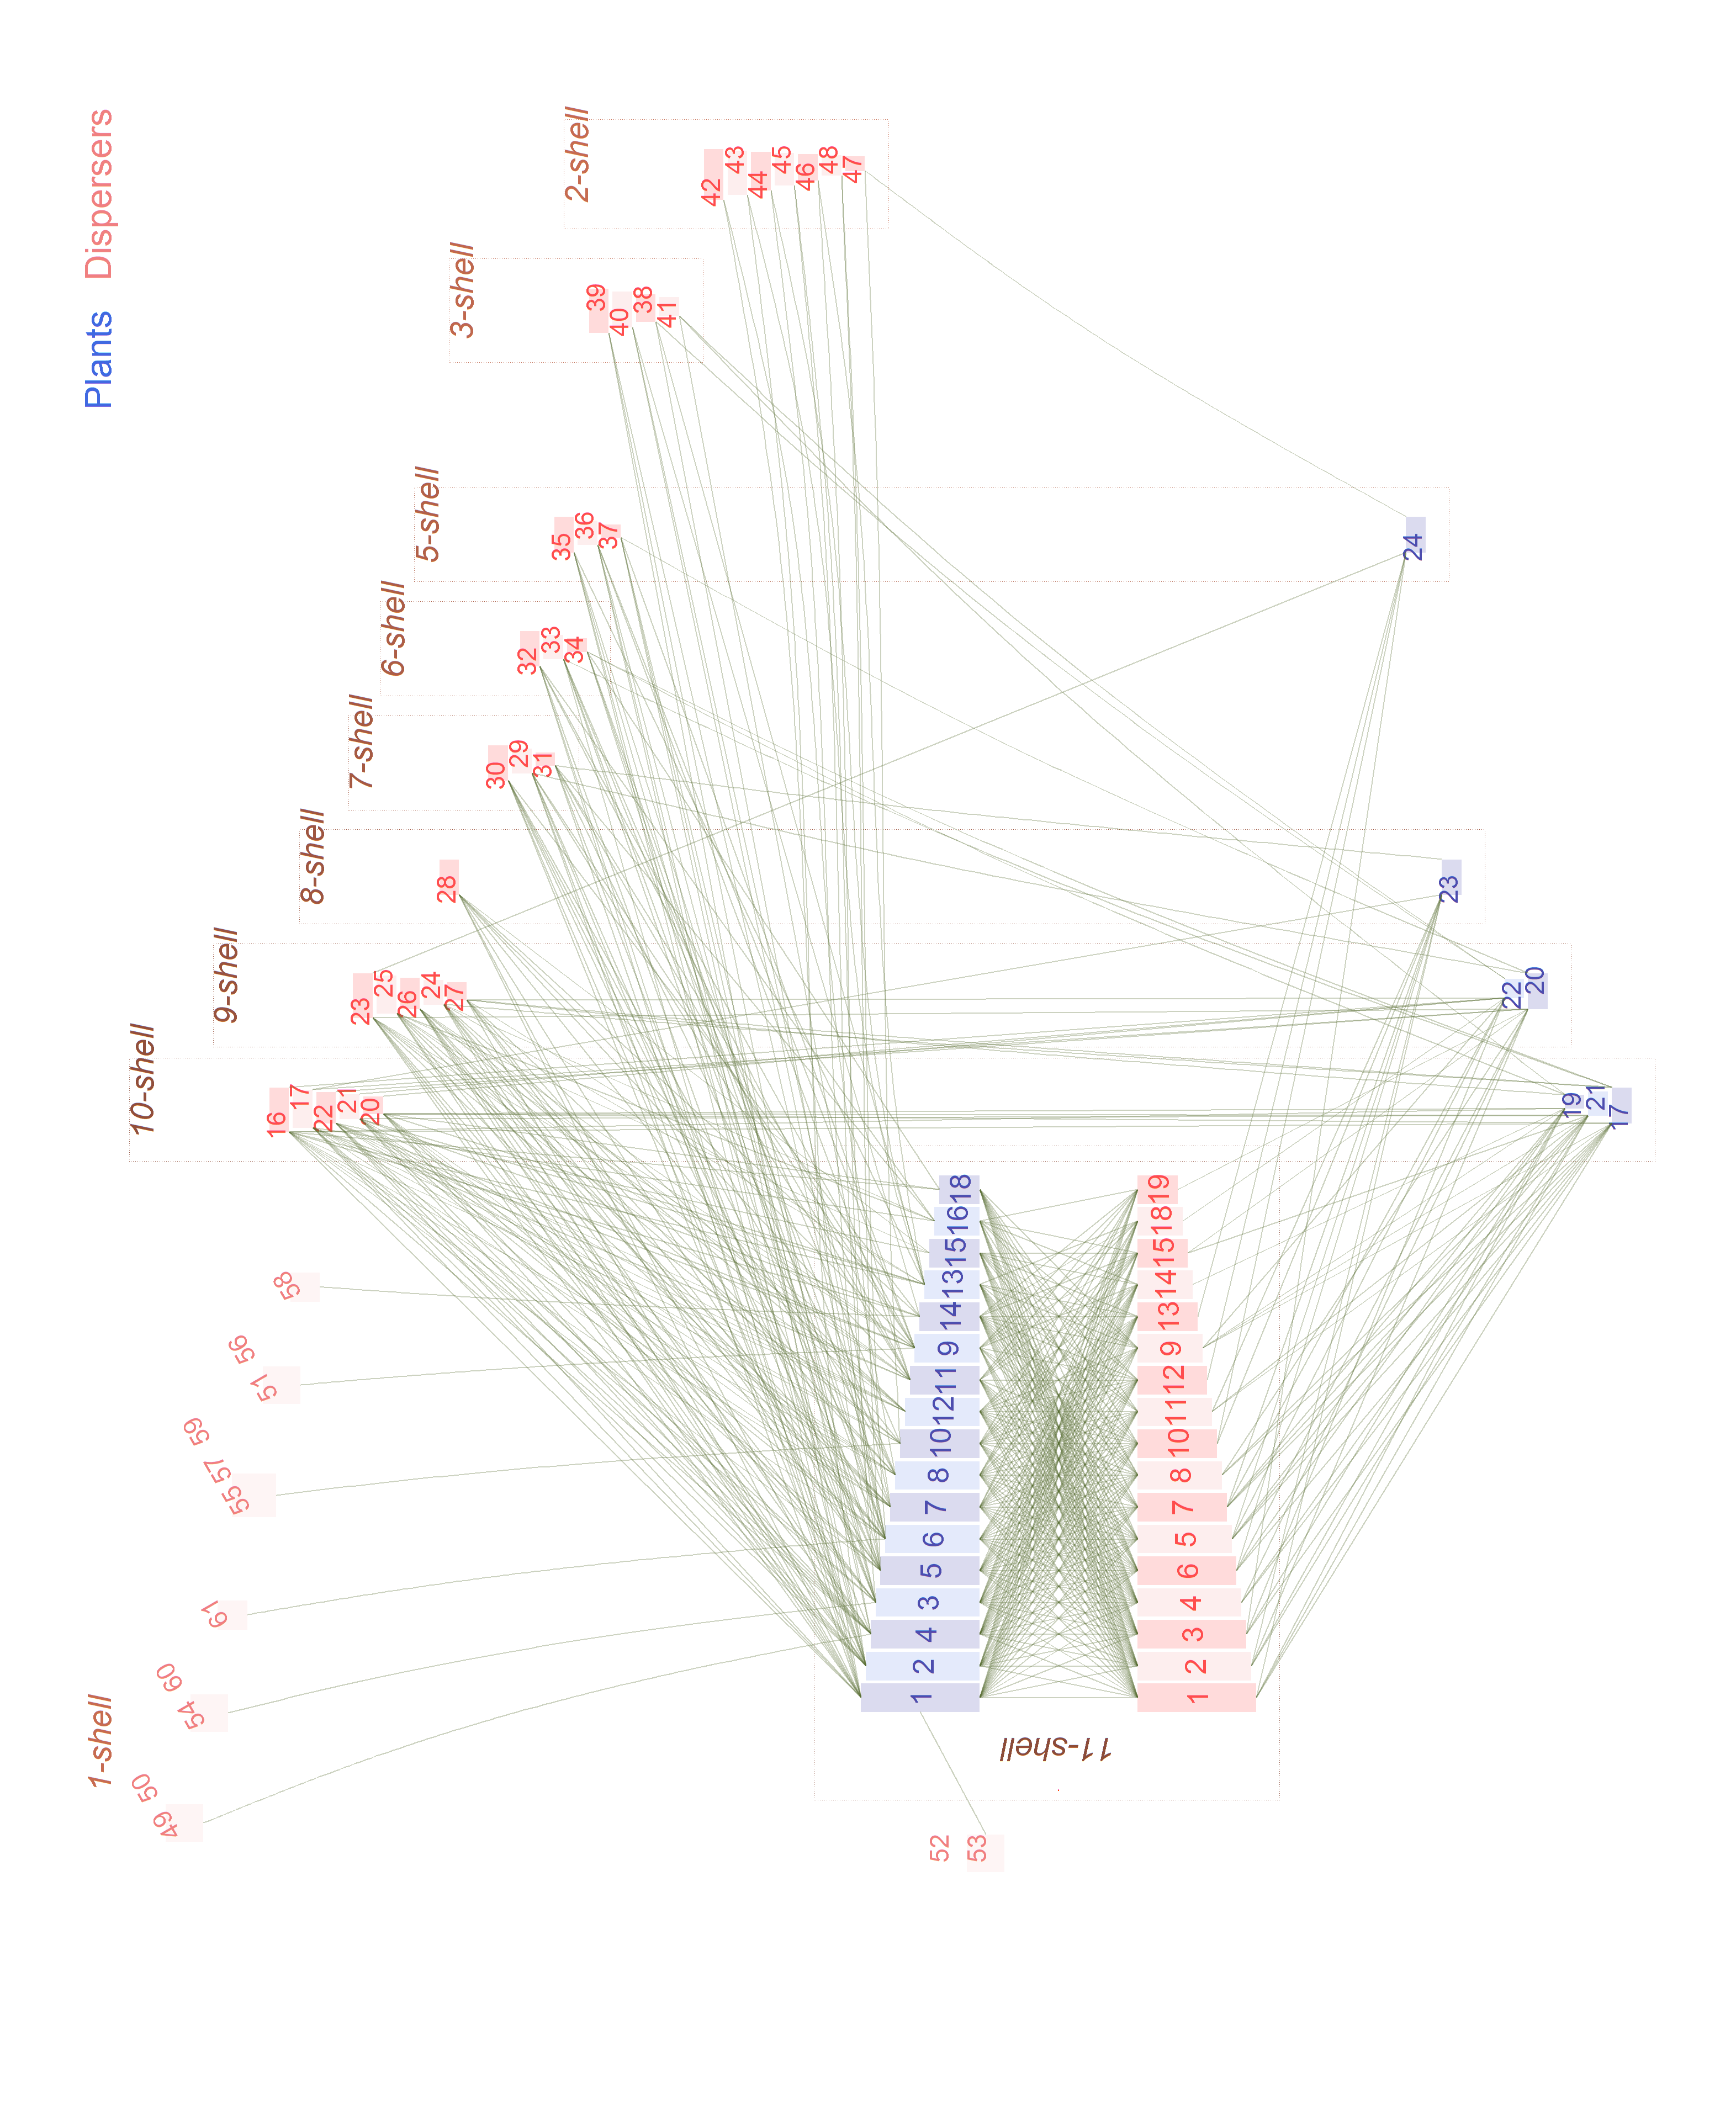
\includegraphics[scale=0.20]{Figures/VIS_M_SD_016_ziggurat.png}
\caption {Red de aves frugívoras $M\_SD\_016$ en la selva Kuala Lompat, Reserva de Krau Game, Malasia \cite{lambert1989fig}, con $85$ especies y $500$ enlaces.}
\label{fig:VIS_M_SD_016_ziggurat}
\end{figure}

\clearpage
\begin{figure}[ht!]
\centering
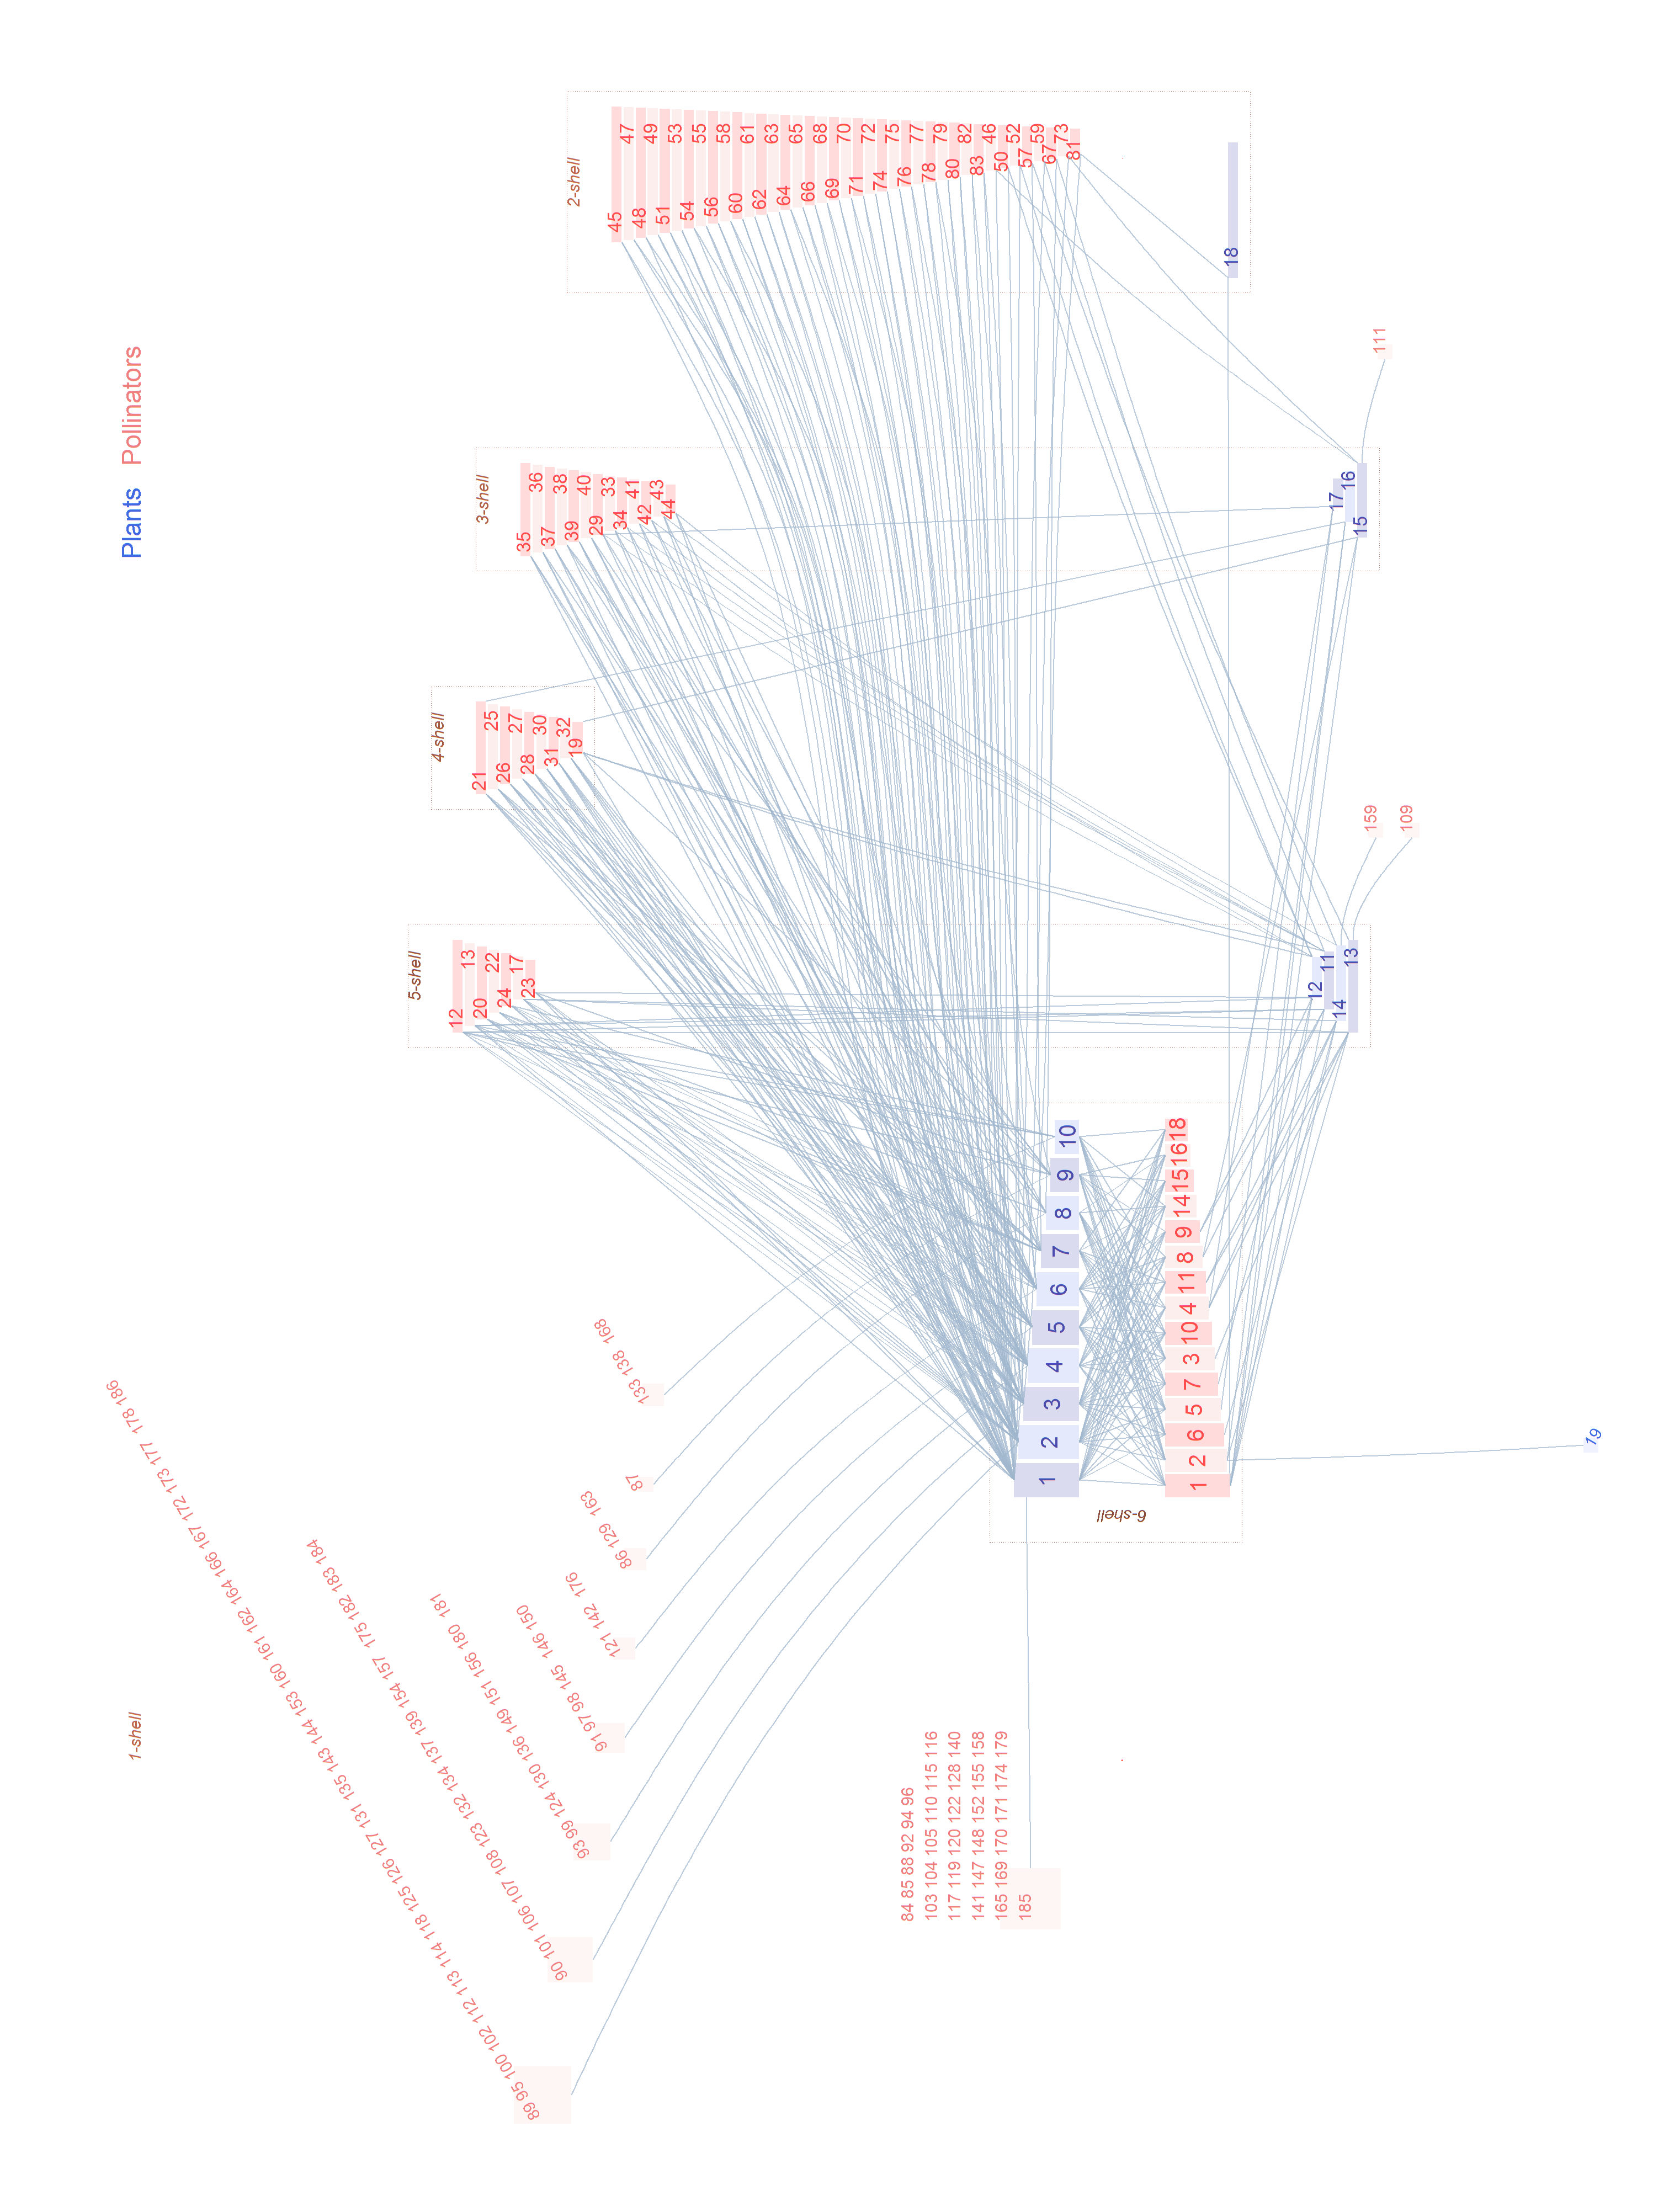
\includegraphics[scale=0.20]{Figures/VIS_M_PL_047_ziggurat.png}
\caption {Red de polinizadores $M\_PL\_047$, de un brezal en Isen Bjerg, Dinamarca \cite{dupont2009ecological}, con $205$ especies y $425$ enlaces.}
\label{fig:VIS_M_PL_047_ziggurat}
\end{figure}


\clearpage
\section{Visualización de la estructura}

El diagrama zigurat no solo sirve para captar la riqueza y variedad de las comunidades mutualistas, también puede ayudar a entender algunas de sus propiedades. En el capítulo precedente se llevó a cabo un análisis de modelo nulo que reveló importantes diferencias en las redes de la colección \ref{fig:ESTATICA_zscore_all}. Se comprobó que la mayoría de las que tienen matriz de adyacencia pesada no son significativamente anidadas usando un modelo nulo restrictivo. Pese a ello, tres sí mostraban fuerte anidamiento y una de ellas además era compacta, la red de polinizadores $059$ (figura \ref{fig:VIS_M_PL_059_ziggurat}).

\begin{figure}[h!]
\centering
\includegraphics[scale=0.42]{Figures/VIS_M_PL_059_ziggurat.png}
\caption {Red de polinizadores $M\_PL\_059$, Parque Nacional do Catimbau, Brasil, con $26$ especies y $71$ enlaces \cite{bezerra2009pollination}. $NODF = 76,88$, $\overline {k}_{radius} = 1,57$ .}
\label{fig:VIS_M_PL_059_ziggurat}
\end{figure}

Con este gráfico se entiende fácilmente por qué $zNODF = 6,84$ y $z \overline {k}_{radius} = -7,34$ alcanzan valores tan extremos. Todas las especies tienen enlaces directos con la \textit{shell} máxima y apenas hay $3$ enlaces entre nodos de la $4$-$shell$. Es un caso de anidamiento y compacidad altísimos.

La red $M\_PL\_024$ (figura \ref{fig:VIS_zig_pl_024}) no es anidada ($zNODF = -1,79$) pero está al límite de ser compacta ($\overline {k}_{radius} = -1,98$). Esta configuración, con forma de campanilla recostada, es bastante habitual y aparece en los procesos de destrucción. Hay un número no despreciable de enlaces dentro de la $2$-$shell$. Esto reduce el valor del anidamiento, pero no afecta al ${k}_{radius}$ de las especies porque tienen también conexión directa con la \textit{shell} máxima.

Entre las redes con matriz binaria la que se sitúa en el extremo de máximo anidamiento y compacidad en la de dispersores de semillas número $016$ (figura \ref{fig:VIS_M_SD_016_ziggurat}). La hemos utilizado como ejemplo en el apartado anterior y es patente como una gran mayoría de los enlaces tienen extremo en la $11$-$shell$. Por esto, los índices reducidos toman también
valores excepcionales: $zNODF = 16,65$ y $\overline {k}_{radius} = -7,99$.

En el extremo opuesto se encuentra la red de polinizadores $031$ (figura \ref{fig:VIS_M_PL_031_ziggurat}), debido a su peculiar configuración de cadenas de especialistas, que hacen que sea anidada ($zNODF = 3,98$), pero no compacta ($\overline {k}_{radius} = 0,22$). Un caso interesante es el de las redes en las que el índice $k$ máximo es $2$, como la de polinizadores número $022$. Son también anidadas ($zNODF = 3,93$) pero no compactas ($\overline {k}_{radius} = 0,58$).

\begin{figure}[h!]
\centering
\includegraphics[scale=0.5]{Figures/VIS_M_PL_022_ziggurat.png}
\caption {Red de polinizadores $M\_PL\_022$, Los Andes, Argentina, con $66$ especies y $83$ enlaces \cite{medan2002plant}. $NODF = 18,02$, $z \overline {k}_{radius} = 3,68$ .}
\label{fig:VIS_M_PL_022_ziggurat}
\end{figure}

\clearpage
En el capítulo anterior también se describió un experimento que consiste en recablear al azar un porcentaje de los enlaces y medir su efecto en la correlación entre $NODF$ y $\overline k_{radius}$ (figura \ref{fig:ESTATICA_histo_corr_rewiring}). La mayoría de las redes experimentan una degradación lineal por la que el anidamiento, medido con $NODF$, decrece y el $\overline k_{radius}$ aumenta. Se llega a un estado similar al que se obtendría si las especies interactuasen al azar, lo que sabemos que está lejos de la realidad.

No obstante, un pequeño porcentaje se salía de este patrón. En general, eran redes pequeñas o con una marcada asimetría. En los dos ejemplos que se incluyen a continuación, los diagramas zigurat permiten entender el por qué de este comportamiento.

El primero (figura \ref{fig:VIS_PL_012}) corresponde a una red de tamaño mediano, con una estructura compleja. La red original se representa con los colores habituales, las correspondientes a los distintos grados de recableado en otros tonos, para recalcar que no se trata de redes reales. 

En la red sin alterar, se observa un índice $k$ máximo de $4$, y una gran conectividad directa con esas \textit{shells}. Hay un importante número de especies en la $1$-$shell$. En el gráfico de correlación general entre $NODF$ y $\overline k_{radius}$ (figura \ref{fig:ESTATICA_corrfigs}) esta red se sitúa en una zona intermedia.

Cuando se reconectan al azar seis enlaces, la estructura cambia poco, aunque puede verse como aparece una $2$-$shell$ de plantas y aumenta la conectividad entre las \textit{k shells} inferiores. Es importante recalcar que esta red alterada es resultado de una realización aleatoria, la configuración puede variar entre distintos intentos, por eso las gráficas de la figura \ref{fig:ESTATICA_corrfigs} se obtuvieron repitiendo veinte veces el recabledado para un mismo número de enlaces. No obstante, un recableado mínimo como el del ejemplo, tiene pocas consecuencias para las medidas globales de esta red.

Al aumentar a diecisiete los enlaces reconectados, la degradación es más notable. El índice $k$ máximo baja a $3$. Si sigue creciendo la cantidad de reconexiones, la modificación es aun más evidente. En la imagen, para treinta y dos cambios al azar, las $2$-$shells$ han crecido a costa de la $3$ y aparecen muchas más conexiones, en proporción, entre ellas. La $NODF$ ha bajado desde el original $30,40$ a $12,22$ y el $\overline k_{radius}$ pasa de $2,51$ a $2,82$.

Obsérvese la forma de campanilla recostada que revela el diagrama zigurat de la red con la mitad de sus enlaces recableados, con  muchas conexiones entre especies de la $2$-$shell$. Esta figura es la de una red mutualista poco estructurada.

En el segundo ejemplo se presenta un caso extremo de comportamiento fuera de la norma  (figura \ref{fig:VIS_SD_007}). Esta red de frugívoros es muy asimétrica con solo $7$ especies de plantas por $72$ de animales. Las especies $1$ a $6$ de plantas forman la $3$-$shell$, solo la número $7$ tiene un lugar marginal en la $1$-$shell$.

\clearpage
\begin{figure}[ht!]
\centering
\includegraphics[scale=0.80]{Figures/VIS_PL_012.pdf}
\caption {Red de polinizadores $M\_PL\_012$, en el Parque Nacional de Garajonay, La Gomera (España), compilada por Olesen y no publicada, con $84$ especies y $145$ enlaces. Arriba, la red original, $NODF = 30,40$, $\overline k_{radius} = 2,51$. En sentido horario, red con siete enlaces recableados al azar, $NODF = 26,62$, $\overline k_{radius} = 2,48$; con diecisiete enlaces recableados, $NODF = 22,62$, $\overline k_{radius} = 2,77$ y con treinta y dos, $NODF = 13,22$, $\overline k_{radius} = 2,82$.}
\label{fig:VIS_PL_012}
\end{figure}

\clearpage
\begin{figure}[ht!]
\centering
\includegraphics[scale=0.8]{Figures/VIS_SD_007.pdf}
\caption {Red de frugívoros $M\_SD\_007$, en el norte de Queensland, Australia \cite{crome1975ecology}, con $79$ especies y $143$ enlaces. Arriba, la red original, $NODF = 51,67$, $\overline k_{radius} = 2,37$. Abajo, red con seis enlaces recableados al azar, $NODF = 44,75$, $\overline k_{radius} = 2,09$. En el centro el comportamiento de los índices reducidos ante el proceso de recableado.}
\label{fig:VIS_SD_007}
\end{figure}

\clearpage
Con esta configuración parece claro que una alteración mínima de las conexiones de las plantas tendrá un impacto sensible en la estructura global. Es lo que sucede recableando al azar solo seis enlaces. Aparece una $4$-$shell$ y disminuyen a la vez $NODF$ y  $\overline k_{radius}$. En el diagrama de correlación de los índices reducidos se ve que cualquier cambio disminuye el primer parámetro, pero esa información no basta para intuir los profundos cambios de estructura que se desencadenan.

Una situación real en la que las redes cambian de forma drástica se produce por la extinción de una o más especies. En la figura \ref{fig:VIS_M_SD_004_pol3_pol4_ziggurat} se representa la red $M\_SD\_004$ (figura \ref{fig:ziggurat}), en la que se han eliminado únicamente los dos polinizadores de mayor $k_{degree}$, los números $3$ y $4$. El resultado es la reducción en $1$ del índice $k$ máximo, $NODF$ baja desde $39,82$ a $22,46$ y $\overline k_{radius}$ pasa de $2,19$ a $2,26$. La degradación de la red se asemeja a la que se ha visto con el experimento de recableado, con la fusión del $k$ máximo con el $k$-$1$ y el crecimiento de la proporción de enlaces entre especies fuera del $k$ máximo resultante. La red resultante adopta la ya conocida forma de campanilla.

\begin{figure}[ht!]
\centering
\includegraphics[scale=0.5]{Figures/VIS_M_SD_004_pol3_pol4_ziggurat.png}
\caption {Red de frugívoros $M\_SD\_004$, en la que se han eliminado los polinizadores números $3$ y $4$, los dos de mayor $k_{degree}$, véase la figura \ref{fig:ziggurat}.} 
\label{fig:VIS_M_SD_004_pol3_pol4_ziggurat}
\end{figure}

\clearpage
\begin{figure}[ht!]
\centering
\includegraphics[scale=0.33]{Figures/VIS_M_SD_004_minus_k4_ziggurat.png}
\caption {Red de frugívoros $M\_SD\_004$, en la que se han eliminado todos los polinizadores de la $4$-$shell$, véase la figura \ref{fig:ziggurat}.} 
\label{fig:VIS_M_SD_004_minus_k4_ziggurat}
\end{figure}

\begin{figure}[h!]
\centering
\includegraphics[scale=0.45]{Figures/VIS_M_SD_018_ziggurat.png}
\caption {Red de frugívoros $M\_SD\_018$, en Papúa Nueva Guinea \cite{mack1996notes}.} 
\label{fig:VIS_M_SD_018_ziggurat}
\end{figure}

El diagrama de zigurat permite ver de forma clara la importancia de la \textit{shell} máxima para la estabilidad de la red. Si en la misma red  $M\_SD\_004$ desaparecieran todas las especies de polinizadores de la $4$-$shell$ de manera simultánea ($1$,$3$,$4$,$5$ y $8$) el resultado sería casi catastrófico para la comunidad. El anidamiento cae a $NODF = 3,38$. La red sobreviviente es un pequeño núcleo en $2$-$shell$ y escasas especies en $1$-$shell$ (figura \ref{fig:VIS_M_SD_004_minus_k4_ziggurat}).

En la figura \ref{fig:VIS_Modvskdegree3-sd04} se han representado los diagramas polares de la red intacta, de la red sin los dos polinizadores y de la red sin la $4$-$shell$ y el gráfico de la relación de $\overline k_{degree}$ con $Modularity$ como se hizo en la figura \ref{fig:VIS_Modvskdegree3-sd04}. Desde una posición inicial en la mitad del gráfico, los dos estados degradados se desplazan hacia posiciones de menor $k_{degree}$ y mayor $Modularity$.

\begin{figure}[h!]
\centering
\includegraphics[scale=0.23]{Figures/VIS_Modvskdegree3-sd04.pdf}
\caption {Diagramas polares de la red $M\_SD\_004$ intacta, tras eliminar los dos polinizadores de mayor $k_{degree}$ y tras suprimir la $4$-$shell$ de polinizadores completa.} 
\label{fig:VIS_Modvskdegree3-sd04}
\end{figure}
 
\clearpage
\begin{figure}[ht!]
\centering
\includegraphics[scale=0.5]{Figures/VIS_M_SD_004_minus_k3k2_ziggurat.png}
\caption {Red de frugívoros $M\_SD\_004$, en la que se han eliminado todos los polinizadores de la $3$-$shell$ ($NODF = 36,24$, $\overline k_{radius} = 2,17$) y la $2$-$shell$ ($NODF = 33,055$, $\overline k_{radius} = 2,15$), véase la figura \ref{fig:ziggurat}.} 
\label{fig:VIS_M_SD_004_minus_k3k2_ziggurat}
\end{figure}

\clearpage
Cabe preguntarse si las redes resultantes de las extinciones se parecen a redes reales. La de toda la colección cuyos parámetros se acercan más a la de la figura \ref{fig:VIS_M_SD_004_minus_k4_ziggurat} es una comunidad de frugívoros que en estado natural tiene un $k$ máximo $2$ (figura \ref{fig:VIS_M_SD_018_ziggurat}). Se ha señalado en el gráfico de correlación de \ref{fig:VIS_Modvskdegree3-sd04} la posición de esta red.

Su aspecto general es muy similar al de lo que queda de la comunidad de Puerto Rico al extinguirse los frugívoros de la \textit{shell} máxima. Esto lleva a pensar que las comunidades mutualistas con bajos índices $k$ máximos pueden ser restos de otras anteriores más complejas que han perdido parte de sus nodos. Alternativamente, podrían ser estados iniciales de formación.

Se ha comprobado como afecta a la red $M\_SD\_004$ la pérdida de los cinco frugívoros de la \textit{shell} máxima, ¿qué ocurre si ese núcleo se mantiene y se destruyen los de índices $k$ menores?

En la imagen superior de la figura \ref{fig:VIS_M_SD_004_minus_k3k2_ziggurat}, se han extinguido las dos especies de frugívoros que formaban la $3$-$shell$. La $NODF$ baja muy poco, de $39,82$ a $36,34$ y el $\overline k_{radius}$ prácticamente no se modifica. El contraste es grande si se compara con el resultado de eliminar los dos frugívoros de mayor $\overline k_{degree}$, tanto en el porcentaje de cambio de las magnitudes como en el de la estructura de la red. Se sigue conservando el índice $k$ máximo $4$.

Si a continuación se extinguen las cuatro especies animales de la $2$-$shell$, tampoco se observan grandes cambios en los parámetros de la red resultante (figura \ref{fig:VIS_M_SD_004_minus_k3k2_ziggurat}, abajo). Esto es así porque los frugívoros desaparecidos tenían casi todos sus enlaces con la $4$-$shell$ de plantas, como consecuencia del anidamiento. Apenas hay arrastre de otras especies (solo las dos plantas de la $1$-$shell$ conectadas a la $3$-$shell$ de animales).

Con este ejemplo se puede entender mejor la importancia del orden de extinción basándose únicamente en el orden de las \textit{k-shells}. Si se conservan las \textit{shells} máximas y la red está bien anidada, la pérdida de otras \textit{shells} de índice inferior no arrastra apenas otras especies. Por el contrario, si hay muchos enlaces entre entre estas \textit{shells} inferiores, el fenómeno puede propagarse dando origen a las extinciones en cascada y la red en conjunto resulta más frágil. En el siguiente capítulo se describe con detalle la influencia de la \textit{k-estructura} en la resistencia de la red.

La conservación de las especies de las \textit{shells} máximas debe ser prioritaria porque de ellas depende en gran medida la supervivencia de toda la comunidad, y el diagrama zigurat es una ayuda gráfica para la comprensión de este hecho.

%\section{Conclusiones}
%
%La visualización de datos es una gran ayuda para la investigación, porque permite observar detalles estructurales. Para ello, las herramientas gráficas deben estar adaptadas a las propiedades de la información. Los gráficos más usados en el estudio de las comunidades mutualistas se vuelven muy confusos cuando la red tiene unas pocas decenas de especies. 
%
%La descomposición \textit{k core} ha permitido definir dos nuevos diagramas, denominados polar y zigurat. El diagrama polar utiliza la descomposición
%como mecanismo de reducción de la información. Permite percibir en qué grado la red es jerárquica y es útil para comparar redes con independencia de sus tamaños.
%
%El diagrama zigurat es más rico. Se representan todas las especies y enlaces y revela con claridad la estructura de \textit{k shells}. Tiene aplicación para comparar la evolución temporal de una red, ya sea por extinciones parciales, por experimentos de reconfiguración o por cualquier otra circunstancia que altere el número de especies y su conectividad. Los diagramas de zigurat tienden a adoptar una serie de figuras tipo que permiten deducir a simple vista algunas propiedades de la red.

\section{Anexo: Gráficos de la colección}

Desde la siguiente dirección puede descargarse un documento con los gráficos de todas las redes de la colección:

\url{https://www.dropbox.com/home/Public?preview=all_networks.pdf}

\section{Anexo: Red del Parque Nacional de Canaima}
\label{ESTATICA_ANEXO_Canaima}
% Table generated by Excel2LaTeX from sheet 'pl31_indiv'
\begin{table}[htbp]
\fontsize{3mm}{3mm}\selectfont
  \centering

    \begin{tabular}{lrrrlrr}
    \toprule
    $Especie$ & $k_{radius}$ & $k_{degree}$ &      & $Especie$ & $k_{radius}$ & $k_{degree}$ \\
    \midrule
    Planta1 & 2,20 & 5,00 &      & Polinizador1 & 1,00 & 9,80 \\
    Planta2 & 1,00 & 5,96 &      & Polinizador2 & 2,33 & 6,37 \\
    Planta3 & 1,00 & 5,53 &      & Polinizador3 & 1,00 & 7,21 \\
    Planta4 & 3,80 & 1,93 &      & Polinizador4 & 1,00 & 6,75 \\
    Planta5 & 1,00 & 5,53 &      & Polinizador5 & 3,00 & 2,80 \\
    Planta6 & 4,20 & 1,67 &      & Polinizador6 & 1,67 & 5,39 \\
    Planta7 & 2,60 & 3,00 &      & Polinizador7 & 3,00 & 1,81 \\
    Planta8 & 1,00 & 5,46 &      & Polinizador8 & 1,00 & 5,43 \\
    Planta9 & 3,00 & 1,79 &      & Polinizador9 & 2,00 & 3,72 \\
    Planta10 & 1,80 & 3,36 &      & Polinizador10 & 3,00 & 1,55 \\
    Planta11 & 1,40 & 4,00 &      & Polinizador11 & 3,00 & 1,58 \\
    Planta12 & 4,20 & 1,20 &      & Polinizador12 & 4,33 & 1,07 \\
    Planta13 & 1,40 & 4,00 &      & Polinizador13 & 3,00 & 1,41 \\
    Planta14 & 2,60 & 2,10 &      & Polinizador14 & 5,00 & 0,65 \\
    Planta15 & 2,60 & 2,10 &      & Polinizador15 & 3,00 & 1,17 \\
    Planta16 & 4,20 & 0,87 &      & Polinizador16 & 3,00 & 0,96 \\
    Planta17 & 2,20 & 2,03 &      & Polinizador17 & 3,00 & 0,84 \\
    Planta18 & 2,60 & 1,76 &      & Polinizador18 & 3,00 & 1,01 \\
    Planta19 & 4,20 & 0,76 &      & Polinizador19 & 3,00 & 1,08 \\
    Planta20 & 2,60 & 1,67 &      & Polinizador20 & 3,00 & 1,10 \\
    Planta21 & 4,60 & 0,73 &      & Polinizador21 & 5,00 & 0,48 \\
    Planta22 & 2,60 & 1,93 &      & Polinizador22 & 5,00 & 0,40 \\
    Planta23 & 2,60 & 1,33 &      & Polinizador23 & 2,33 & 2,00 \\
    Planta24 & 3,40 & 0,56 &      & Polinizador24 & 5,00 & 0,50 \\
    Planta25 & 6,20 & 0,34 &      & Polinizador25 & 2,33 & 2,00 \\
    Planta26 & 4,20 & 0,67 &      & Polinizador26 & 3,00 & 0,72 \\
    Planta27 & 3,40 & 0,67 &      & Polinizador27 & *    & * \\
    Planta28 & 3,40 & 0,53 &      & Polinizador28 & *    & * \\
    Planta29 & 2,60 & 1,43 &      & Polinizador29 & 5,00 & 0,24 \\
    Planta30 & 2,60 & 0,87 &      & Polinizador30 & 5,00 & 0,22 \\
    Planta31 & 3,00 & 0,76 &      & Polinizador31 & *    & * \\
    Planta32 & *    & *    &      & Polinizador32 & *    & * \\
    Planta33 & 4,60 & 0,53 &      & Polinizador33 & 5,00 & 0,24 \\
    Planta34 & 2,60 & 1,33 &      & Polinizador34 & 3,00 & 0,38 \\
    Planta35 & *    & *    &      & Polinizador35 & 4,33 & 0,33 \\
    Planta36 & 4,60 & 0,53 &      & Polinizador36 & 5,00 & 0,24 \\
    Planta37 & 5,00 & 0,39 &      & Polinizador37 & 4,33 & 0,33 \\
    Planta38 & 2,60 & 1,43 &      & Polinizador38 & 7,00 & 0,16 \\
    Planta39 & 2,60 & 1,43 &      & Polinizador39 & 5,00 & 0,22 \\
    Planta40 & 5,40 & 0,20 &      & Polinizador40 & 5,00 & 0,24 \\
    Planta41 & 2,60 & 1,00 &      & Polinizador41 & 5,00 & 0,24 \\
    Planta42 & 5,80 & 0,20 &      & Polinizador42 & 3,67 & 0,38 \\
    Planta43 & 3,40 & 0,33 &      & Polinizador43 & 3,00 & 0,38 \\
    Planta44 & 4,60 & 0,33 &      & Polinizador44 & 5,00 & 0,24 \\
    Planta45 & 4,60 & 0,33 &      & Polinizador45 & 3,00 & 0,45 \\
    Planta46 & 3,00 & 0,50 &      & Polinizador46 & 3,00 & 0,45 \\
    Planta47 & 2,60 & 1,00 &      & Polinizador47 & 6,33 & 0,20 \\
    Planta48 & 3,40 & 0,33 &      & Polinizador48 & 5,00 & 0,26 \\
         &      &      &      & Polinizador49 & 5,00 & 0,22 \\
    \bottomrule
    \end{tabular}%
    \caption{\label{table:kmag_pl_031} \textit{k magnitudes} de la red  de polinizadores $M\_PL\_031$ del Parque Nacional de Canaima, Venezuela, \cite{ramirez1989biologia}. Valores globales: $\overline k_{radius} = 3,39$; $\overline k_{degree} = 1,57$. Las especies desconectadas de la componente gigante aparecen señaladas con asterisco.}
\end{table}%
% Chapter Template

\chapter{Conclusiones de la tesis} % Main chapter title

\label{chapterCONCLUSIONES} % Change X to a consecutive number; for referencing this chapter elsewhere, use \ref{ChapterX}

%----------------------------------------------------------------------------------------
%	SECTION 1
%----------------------------------------------------------------------------------------

\section{XXXX mutualismo}

Lorem ipsum dolor sit amet, consectetur adipiscing elit. Aliquam ultricies lacinia euismod. Nam tempus risus in dolor rhoncus in interdum enim tincidunt. Donec vel nunc neque. In condimentum ullamcorper quam non consequat. Fusce sagittis tempor feugiat. Fusce magna erat, molestie eu convallis ut, tempus sed arcu. Quisque molestie, ante a tincidunt ullamcorper, sapien enim dignissim lacus, in semper nibh erat lobortis purus. Integer dapibus ligula ac risus convallis pellentesque.


%----------------------------------------------------------------------------------------
%	THESIS CONTENT - APPENDICES
%----------------------------------------------------------------------------------------
%\renewcommand{\appendixname}{Apéndice}
%\appendix % Cue to tell LaTeX that the following "chapters" are Appendices

% Include the appendices of the thesis as separate files from the Appendices folder
% Uncomment the lines as you write the Appendices

%% Appendix A

\chapter{Apéndice: Fuentes de datos} % Main appendix title

\label{APP_DATOS} % For referencing this appendix elsewhere, use \ref{AppendixA}

\section{Redes mutualistas del capítulo \label{ChapterESTATICA}}
%\input{Appendices/AppendixB}
%\input{Appendices/AppendixC}

%----------------------------------------------------------------------------------------
%	BIBLIOGRAPHY
%----------------------------------------------------------------------------------------
\renewcommand{\bibname}{Bibliografía}
\printbibliography[heading=bibintoc]

%----------------------------------------------------------------------------------------

\end{document}  
